% GCURS 2026 talk (Computational & Applied Mathematics section), 12 min.
% Build:   latexmk -pdf talk.tex                     -> talk.pdf (slides)
%          pdflatex -jobname=talk_notes "\def\withnotes{}% GCURS 2026 talk (Computational & Applied Mathematics section), 12 min.
% Build:   latexmk -pdf talk.tex                     -> talk.pdf (slides)
%          pdflatex -jobname=talk_notes "\def\withnotes{}% GCURS 2026 talk (Computational & Applied Mathematics section), 12 min.
% Build:   latexmk -pdf talk.tex                     -> talk.pdf (slides)
%          pdflatex -jobname=talk_notes "\def\withnotes{}% GCURS 2026 talk (Computational & Applied Mathematics section), 12 min.
% Build:   latexmk -pdf talk.tex                     -> talk.pdf (slides)
%          pdflatex -jobname=talk_notes "\def\withnotes{}\input{talk}"   (x2)
%                                                    -> talk_notes.pdf (slides + speaker notes)
% Figures: ../figures (make_slide_figures.py) and ../../poster_2026-10-02.
\documentclass[aspectratio=169,11pt]{beamer}
\usetheme{default}
\usepackage{lmodern}
\setbeamertemplate{navigation symbols}{}
\setbeamertemplate{blocks}[rounded][shadow=false]
\setbeamertemplate{footline}[frame number]
\setbeamertemplate{itemize items}[circle]
\usepackage[utf8]{inputenc}
\usepackage[T1]{fontenc}
\usepackage{amsmath,amssymb,bm}
\usepackage{booktabs}
\usepackage{tikz}
\usetikzlibrary{arrows.meta}
\graphicspath{{../figures/}{../../poster_2026-10-02/}{../../}}

\ifdefined\withnotes
  \setbeameroption{show notes}
  \setbeamertemplate{note page}[plain]
\fi

% ---- University of Houston palette (from the UH URD template) ---------------
% UH Red #C8102E, Brick #960C22, Slate #54585A; logos cut from the template's banner.
\definecolor{uhred}{HTML}{C8102E}
\definecolor{uhbrick}{HTML}{960C22}
\definecolor{uhslate}{HTML}{54585A}
\definecolor{navy}{HTML}{231F20}     % primary text (near-black)
\definecolor{ink}{HTML}{54585A}      % secondary text (UH slate)
\definecolor{accent}{HTML}{C8102E}
\definecolor{accentdk}{HTML}{960C22}
\definecolor{paper}{HTML}{FBFBF8}    % matches the figure backgrounds
\definecolor{card}{HTML}{F1F0EE}
\definecolor{vblue}{HTML}{1C5CAB}
\setbeamercolor{normal text}{fg=navy,bg=paper}
\setbeamercolor{frametitle}{fg=white,bg=uhred}
\setbeamercolor{alerted text}{fg=uhred}
\setbeamercolor{block title}{fg=uhbrick,bg=card}
\setbeamercolor{block body}{fg=ink,bg=card}
\setbeamercolor{structure}{fg=uhred}
\setbeamercolor{page number in head/foot}{fg=uhslate}
\setbeamerfont{block title}{size=\small,series=\bfseries}
\setbeamertemplate{frametitle}{%
  \nointerlineskip%
  \begin{beamercolorbox}[wd=\paperwidth,ht=7.5mm,dp=2.8mm,leftskip=4.5mm,rightskip=3.5mm]{frametitle}%
    \usebeamerfont{frametitle}\insertframetitle\hfill\raisebox{-1.7mm}{
\includegraphics[height=6.2mm]{uh/uh_mark_white}}%
  \end{beamercolorbox}%
  \vspace{1mm}}

\newcommand{\takeaway}[1]{\par\smallskip{\color{ink}#1}\par}
\newcommand{\bignum}[2]{{\usebeamerfont{title}\color{navy}\LARGE\bfseries #1}\\[-1pt]{\small\color{ink}#2}}

\title{Brief stops, more vortices}
\subtitle{Deep reinforcement learning discovers transferable control strategies for catalytic-wall Taylor--Couette reactors}
\author{Isaiah N.\ Bascom\inst{1} \and Min Wang\inst{1} \and Yuhe Wang\inst{2}}
\institute{\inst{1}Department of Mathematics, University of Houston, Houston, Texas \and \inst{2}Institute for Scientific Computation, Texas A\&M University, College Station, Texas}
\date{GCURS 2026 \textbullet\ Computational \& Applied Mathematics}

\begin{document}

% ============================================================================
\begin{frame}[plain]
  \begin{tikzpicture}[remember picture,overlay]
    \fill[uhred] (current page.north west) rectangle ([yshift=-15mm]current page.north east);
    \node[anchor=west] at ([xshift=6mm,yshift=-7.5mm]current page.north west) {
\includegraphics[height=9.5mm]{uh/uh_mark_white}};
    \node[anchor=east] at ([xshift=-6mm,yshift=-7.5mm]current page.north east) {
\includegraphics[height=10.5mm]{uh/uh_wordmark_white}};
    \node[anchor=center, text=white, font=\scriptsize\bfseries] at ([yshift=-7.5mm]current page.north) {GCURS 2026 \textbullet\ COMPUTATIONAL \& APPLIED MATHEMATICS};
    \node[anchor=north west, text width=148mm, align=left, inner sep=0pt, text=navy, font=\usebeamerfont{title}\huge\bfseries]
      at ([xshift=6mm,yshift=-20mm]current page.north west) {Brief stops, more vortices};
    \node[anchor=north west, inner sep=0pt, text=ink]
      at ([xshift=6mm,yshift=-31mm]current page.north west) {\resizebox{148mm}{!}{Deep reinforcement learning discovers transferable control strategies for catalytic-wall Taylor--Couette reactors}};
    \node[anchor=north, inner sep=0pt] at ([yshift=-40mm]current page.north)
      {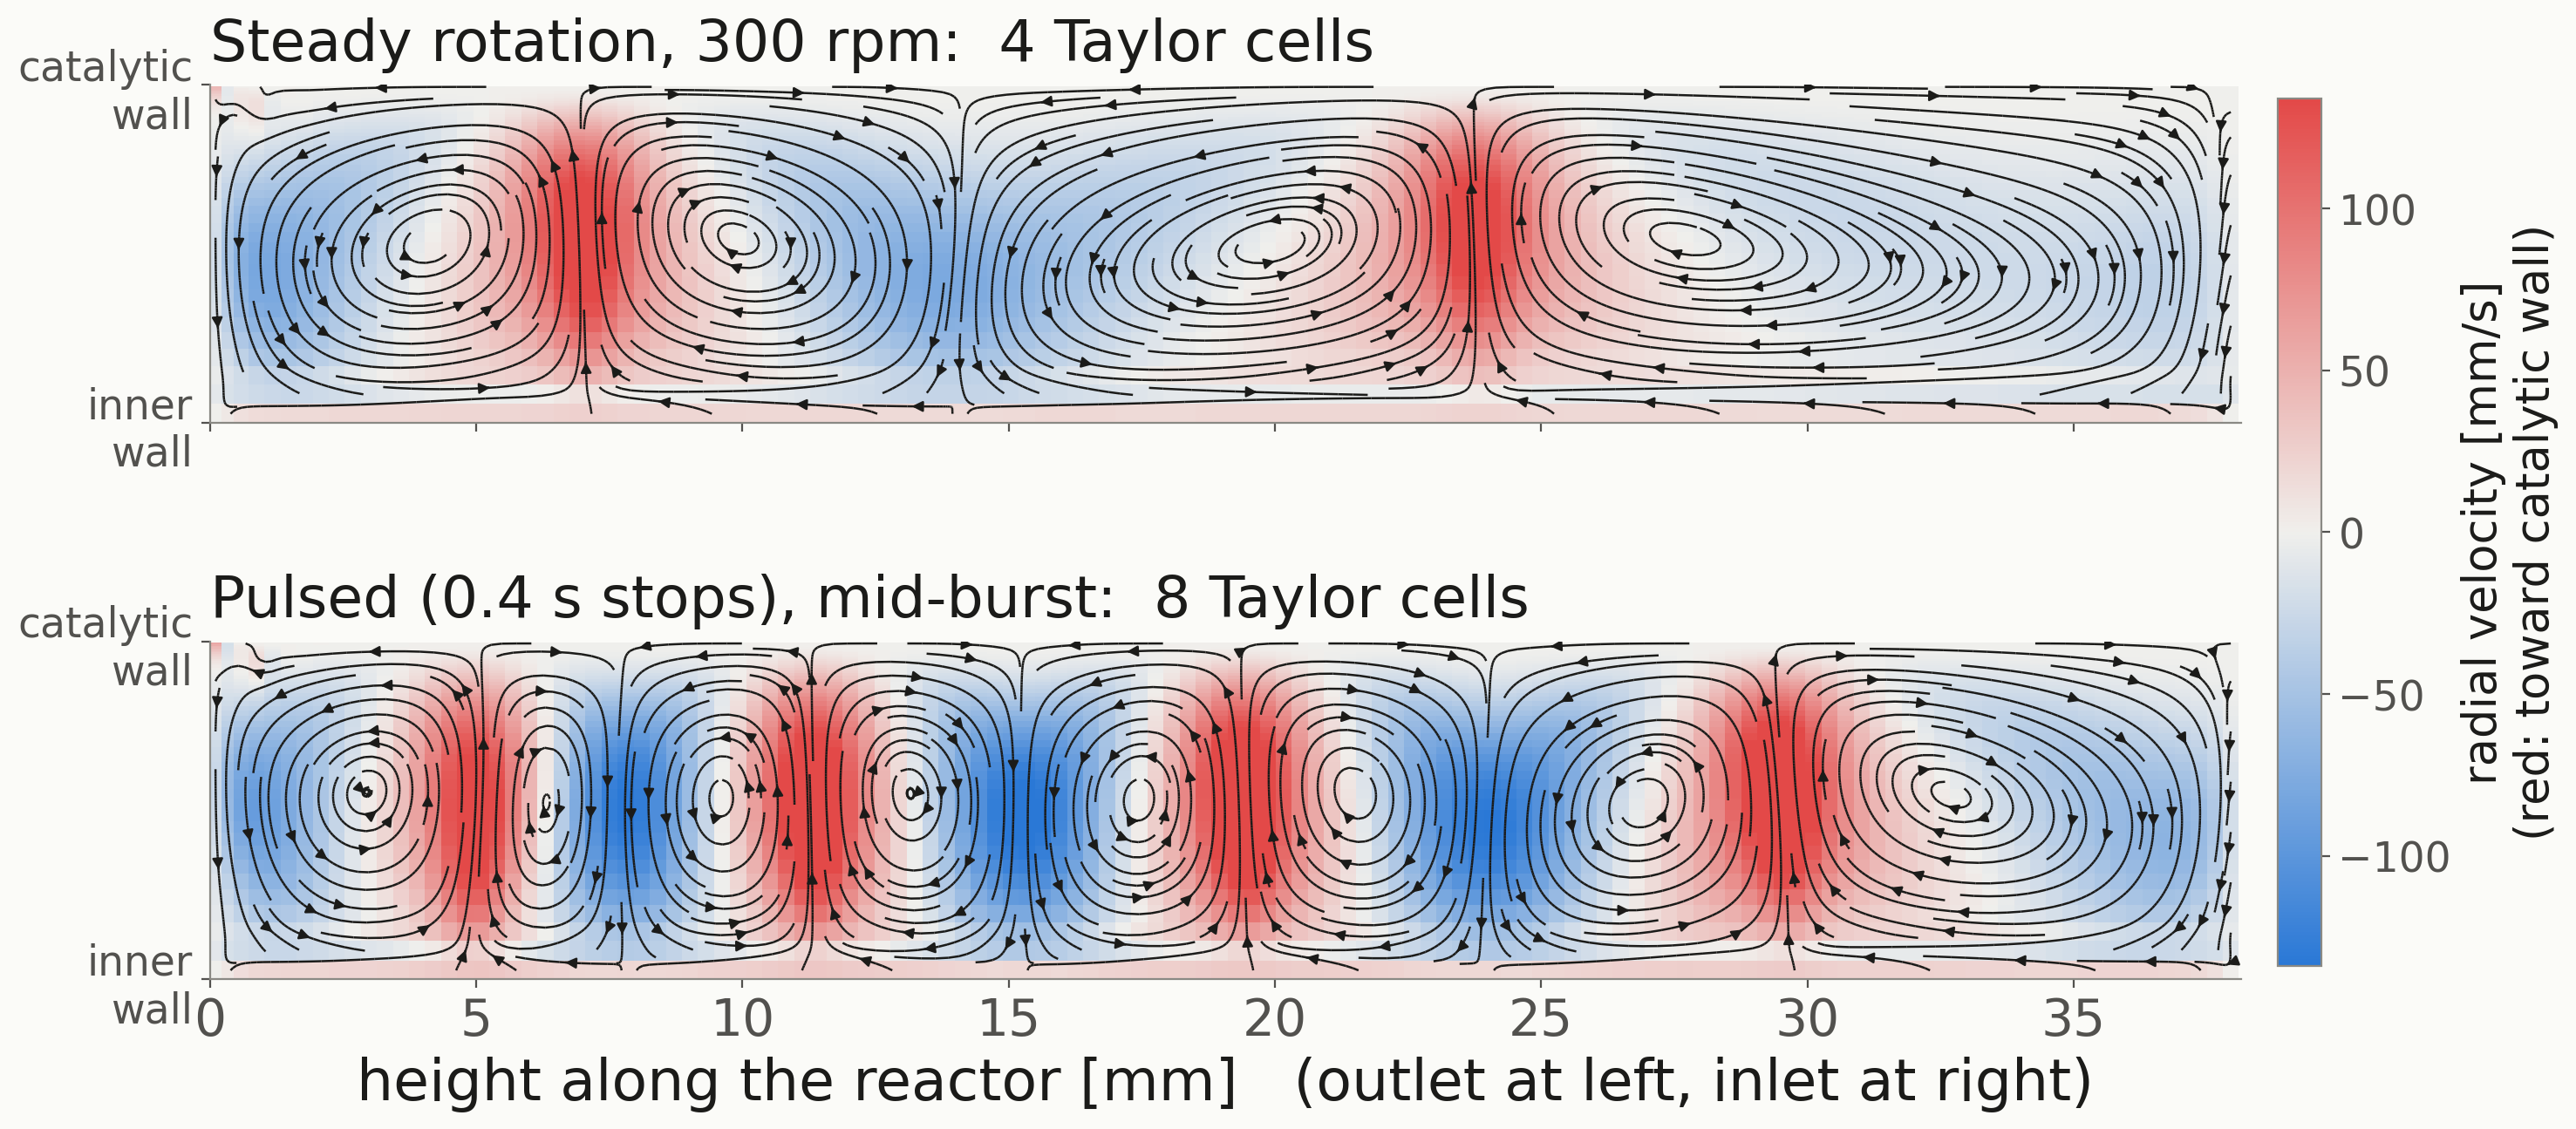
\includegraphics[width=148mm,height=30mm,keepaspectratio]{s_cells_snapshot}};
    \node[anchor=south west, inner sep=0pt, text=navy, font=\bfseries] at ([xshift=6mm,yshift=11.5mm]current page.south west)
      {Isaiah N.\ Bascom$^{1}$, \ Min Wang$^{1}$, \ Yuhe Wang$^{2}$};
    \node[anchor=south west, inner sep=0pt, text=ink, font=\scriptsize, align=left] at ([xshift=6mm,yshift=4mm]current page.south west)
      {$^{1}$Department of Mathematics, University of Houston, Houston, Texas\\
       $^{2}$Institute for Scientific Computation, Texas A\&M University, College Station, Texas};
  \end{tikzpicture}
\end{frame}
\note{[0:30] Hi, I'm Isaiah Bascom. I work on Taylor--Couette reactors: a liquid fills the gap between two cylinders, the inner one spins, and a catalyst coats the outer wall. Today's story has two parts. First, a reinforcement-learning agent found a surprisingly simple way to run this reactor better: brief full stops. Second, we found out why it works. The picture is the punchline: steady rotation gives four vortex cells, and pulsed rotation gives eight.}

% ============================================================================
\begin{frame}{The Taylor--Couette reactor}
  \begin{columns}[c]
    \begin{column}{0.60\textwidth}
      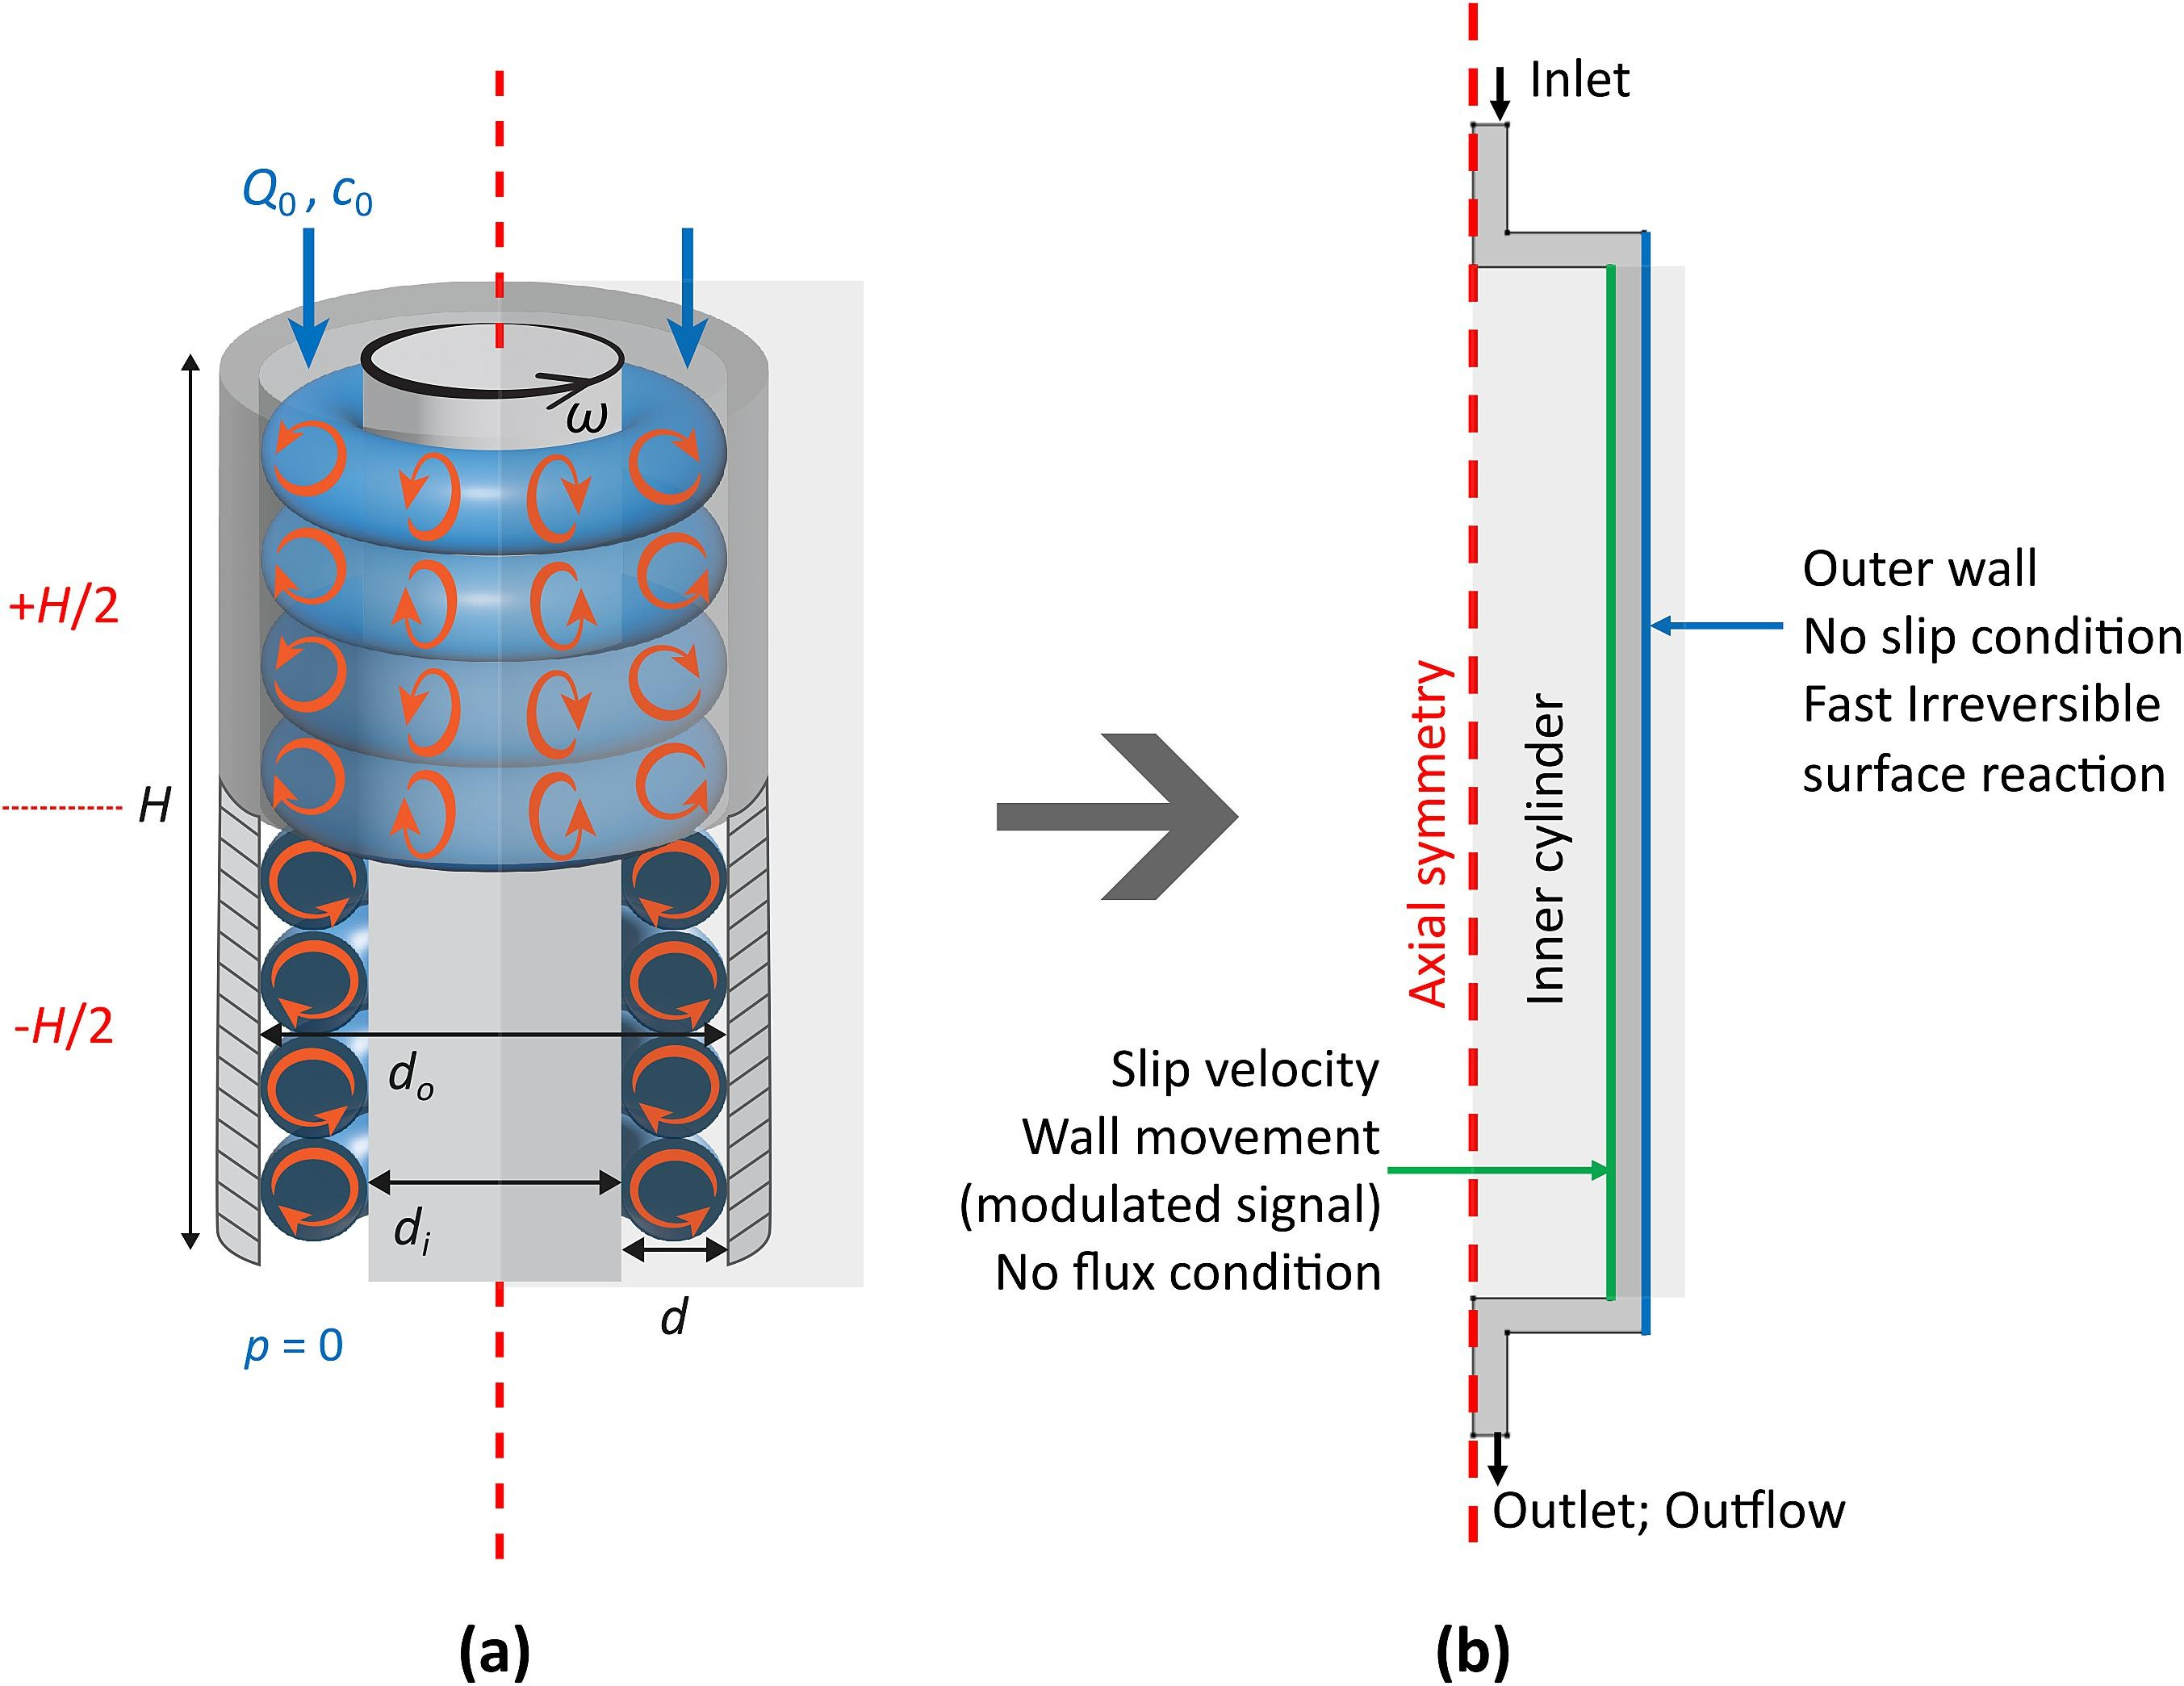
\includegraphics[width=\linewidth,height=0.78\textheight,keepaspectratio]{lg-reactor}\par
      {\tiny\color{ink}Figure: L\'opez-Guajardo et al., \emph{Chem.\ Eng.\ J.} 489 (2024) 151174, Fig.~2.}
    \end{column}
    \begin{column}{0.36\textwidth}
      {\small
      \begin{tabular*}{\linewidth}{@{}l@{\extracolsep{\fill}}r@{}}
        \toprule
        Gap $d$ & 6.35 mm \\
        $d_i$ / $d_o$ & 50.8 / 63.5 mm \\
        Height $H$ & 190.5 mm \\
        $\Gamma = H/d$ & 30 \\
        Feed $Q_0$ & 100 mL/min \\ \bottomrule
      \end{tabular*}}\par\bigskip
      Inner cylinder spins; catalyst on the outer wall.
    \end{column}
  \end{columns}
\end{frame}
\note{[0:45] First, the general setup. A Taylor--Couette reactor is liquid in the gap between two cylinders. The inner one spins, which sets up the stacked ring vortices you see on the left, the Taylor vortices. Feed enters at the top and leaves at the bottom, and the outer wall is coated with catalyst, so the reaction happens only there. The gap is about six millimetres, the reactor is about nineteen centimetres tall, an aspect ratio of thirty. Because the flow is symmetric around the axis, we can simulate just a two-dimensional slice, shown on the right; that's the standard reduction, and it's what makes reinforcement learning on this problem affordable.}

% ============================================================================
\begin{frame}{The reaction happens only at the wall}
  \begin{columns}[c]
    \begin{column}{0.52\textwidth}
      Taylor vortices carry reactant to the catalytic wall.\par\bigskip
      \begin{block}{Problem}
        Choose $\omega(t)$ for the most conversion per unit power.
      \end{block}
    \end{column}
    \begin{column}{0.46\textwidth}
      \centering
      % 2D axisymmetric domain (cf. Lopez-Guajardo et al. Fig. 2b): the fluid gap is the
      % real CFD field under the learned RL policy; everything else is drawn.
      \begin{tikzpicture}[x=1mm, y=1mm, every node/.style={font=\scriptsize}]
        \def\H{46}            % drawn height of the gap [mm]; width = H/6 (true 6.35:38.1)
        \def\W{7.67}
        \def\xg{14}           % left edge of the fluid gap
        % axis of symmetry
        \draw[uhred, dashed, line width=0.8pt] (0,-3) -- (0,\H+4);
        \node[rotate=90, text=uhred, font=\tiny] at (-2.2,\H/2) {axis of symmetry};
        % inner cylinder (schematic, not to scale in r)
        \fill[black!25] (3,0) rectangle (\xg,\H);
        \node[rotate=90, align=center, font=\tiny] at (8.5,\H/2) {inner cylinder, $\omega(t)$};
        % fluid gap: real field
        \node[anchor=south west, inner sep=0] at (\xg,0) {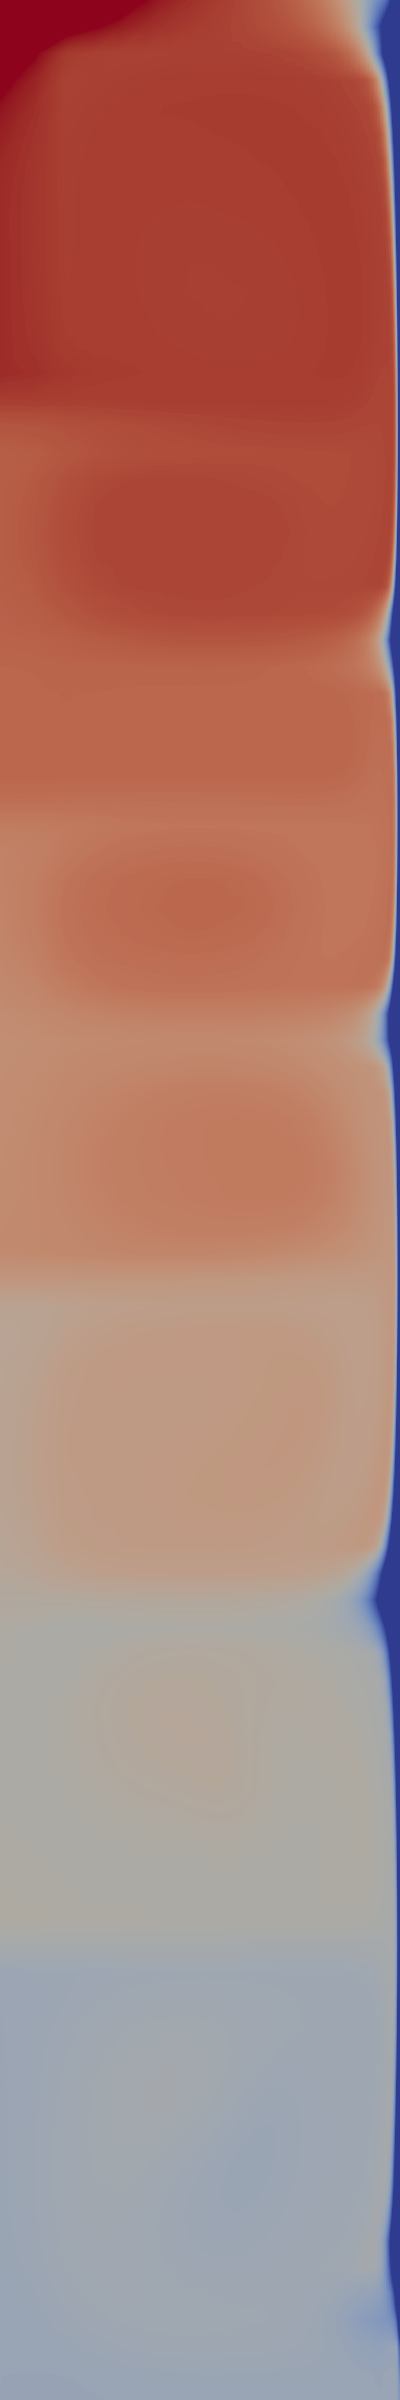
\includegraphics[width=\W mm,height=\H mm]{rl_flow_2d_conc_crop}};
        % bottom wall and catalytic outer wall (outer wall stops above the side outlet)
        \draw[black!60, line width=1.2pt] (\xg,0) -- (\xg+\W,0);
        \definecolor{wallblue}{HTML}{3B4CC0}   % bottom of the concentration scale: c = 0
        \draw[wallblue, line width=1.6pt] (\xg+\W+0.6,1.4) -- (\xg+\W+0.6,\H);
        % inlet at the top of the gap
        \draw[-{Latex[length=2mm]}, navy, line width=1pt] (\xg+\W/2,\H+6) -- (\xg+\W/2,\H+0.6);
        \node[anchor=south] at (\xg+\W/2,\H+6) {inlet};
        % side outlet: the bottom 0.42 mm of the outer wall
        \draw[-{Latex[length=2mm]}, navy, line width=1pt] (\xg+\W+0.2,0.7) -- (\xg+\W+7,0.7);
        \node[anchor=west, align=left] at (\xg+\W+7.3,0.9) {\textbf{side outlet}};
        % labels
        \node[anchor=west, align=left, text=wallblue, font=\scriptsize\bfseries] at (\xg+\W+2.2,\H*0.62)
          {catalytic wall\\[-1pt]{\normalfont\tiny $c = 0$}};
        % concentration key (ParaView "Cool to Warm", matching the render's 0.45-0.88 c/c0 range)
        \definecolor{cw0}{HTML}{3B4CC0}\definecolor{cw1}{HTML}{DDDDDD}\definecolor{cw2}{HTML}{B40426}
        \shade[bottom color=cw0, top color=cw1] (\xg+\W+3,\H*0.22) rectangle (\xg+\W+5,\H*0.32);
        \shade[bottom color=cw1, top color=cw2] (\xg+\W+3,\H*0.32) rectangle (\xg+\W+5,\H*0.42);
        \node[anchor=west, font=\tiny, text=ink] at (\xg+\W+5.4,\H*0.42) {reactant};
        \node[anchor=west, font=\tiny, text=ink] at (\xg+\W+5.4,\H*0.22) {product};
      \end{tikzpicture}\par\smallskip
    \end{column}
  \end{columns}
\end{frame}
\note{[0:45] The reaction only happens on the catalytic outer wall, so everything depends on how fast reactant gets carried from the bulk to that wall. The Taylor vortices in the gap do that carrying. Changing the rotation over time can beat spinning at a constant speed. The picture is the 2D plane our simulation actually solves on, with the real flow under the learned policy: the spinning inner cylinder on the left, the liquid gap coloured by concentration, and the catalytic wall on the right. Red is fresh reactant; blue is where it has been converted to product. You can see the thin blue layer along the catalytic wall, and the vortices peeling that converted liquid off the wall and bringing fresh reactant in. Fluid enters at the top and leaves through a side outlet at the bottom of the outer wall. So this is a control problem governed by PDEs: choose the speed as a function of time to get the most reactant converted for the power spent. What is the optimal control, and why does it work?}

% ============================================================================
\begin{frame}{Non-turbulent flow and scalar transport}
  \begin{columns}[T]
    \begin{column}{0.56\textwidth}
      \begin{block}{Equations}
        \setlength{\abovedisplayskip}{5pt}\setlength{\belowdisplayskip}{5pt}%
        Laminar incompressible flow with constant viscosity and no turbulence model
        \begin{gather*}
          \nabla\cdot\mathbf{u} = 0\\
          \frac{\partial\mathbf{u}}{\partial t} + (\mathbf{u}\cdot\nabla)\mathbf{u} = -\nabla p + \nu\,\nabla^2\mathbf{u}
        \end{gather*}
        Scalar-transport equation
        \[ \frac{\partial c}{\partial t} + \mathbf{u}\cdot\nabla c = D\,\nabla^2 c \]
      \end{block}
    \end{column}
    \begin{column}{0.40\textwidth}
      \begin{block}{Numerics}
        Finite volume (OpenFOAM), 2D axisymmetric; 3330 cells graded to 25\,$\mu$m at the catalytic wall\par\smallskip
        Inner wall: $\omega(t)$\\ Catalytic wall: $c = 0$\\ Inlet: $c = c_0$\par\smallskip
        $\mathrm{Re}\approx 470$, \ $\mathrm{Sc}=1075$
      \end{block}
    \end{column}
  \end{columns}
  \medskip
  \begin{beamercolorbox}[wd=\textwidth,sep=8pt,rounded=true]{frametitle}
    \begin{tabular}{@{}l@{\ }l@{}}
      \textbf{Objective:} & $\max\; X - P/P_{\max}$ \quad s.t. \ $\overline{\omega} = 300$ rpm\\[2pt]
      & {\small $X = 1 - \bar c_{\mathrm{out}}/c_0$ (conversion), \ $P$ = motor power}
    \end{tabular}
  \end{beamercolorbox}
\end{frame}
\note{[0:45] Incompressible Navier--Stokes for the flow, solved axisymmetrically but keeping the swirl component, and an advection--diffusion equation for the reactant. The inner wall turns at a prescribed omega of t. On the catalytic wall the concentration is zero, so the reaction rate is set entirely by how fast reactant diffuses in. Finite-volume discretization in OpenFOAM, with the mesh graded to 25 microns at the wall because the concentration layer there is thin: the Schmidt number is about a thousand. The objective rewards conversion and penalizes motor power. We also fix the mean speed at 300 rpm, which in practice fixes the power, so every candidate is compared at the same power and the question becomes how much conversion each one gets for it.}

% ============================================================================
\begin{frame}{Three ways to search an expensive simulator}
  \begin{columns}[T]
    \begin{column}{0.32\textwidth}
      \begin{block}{\begin{tabular}[t]{@{}l@{\ }l@{}}Discover: & reinforcement\\ & learning\end{tabular}}
        TD3 actor--critic. State: conversion and time. Action: burst and stop lengths. Reward: conversion. No physics given.
      \end{block}
    \end{column}
    \begin{column}{0.32\textwidth}
      \begin{block}{\begin{tabular}[t]{@{}l@{\ }l@{}}Check: & Bayesian\\ & optimization\end{tabular}}
        Gaussian-process surrogate (Mat\'ern-5/2) with expected improvement; 220 CFD runs over fixed waveforms. Replicate noise $\sigma\approx 0.002$.
      \end{block}
    \end{column}
    \begin{column}{0.32\textwidth}
      \begin{block}{\begin{tabular}[t]{@{}l@{\ }l@{}}Explain: & designed\\ & experiments\end{tabular}}
        Pre-registered hypotheses, 62 targeted runs, flow diagnostics logged every 0.02\,s.
      \end{block}
    \end{column}
  \end{columns}
  \bigskip
  \takeaway{Each 130\,s simulation costs about 3--4 CPU-hours, so every method has to be sample-efficient.}
\end{frame}
\note{[0:45] Each simulated episode costs a few CPU-hours, so I used three complementary tools. Reinforcement learning, with TD3, an actor--critic method, to discover a strategy without being told any physics: it sees only the conversion and the time, and chooses how long to run and how long to stop. Bayesian optimization, with a Gaussian-process surrogate and expected improvement over 220 simulations, as an independent check. And designed experiments, with hypotheses written down in advance, to explain why the answer works.}

% ============================================================================
\begin{frame}{Reinforcement learning found brief full stops}
  \alert{All 5 runs: brief full stops (0.1--0.4\,s), never long idles.}\par\medskip
  \centering\includegraphics[width=\linewidth,height=0.66\textheight,keepaspectratio]{fig4_learned_waveform}
\end{frame}
\note{[0:45] Here's what the reinforcement-learning agent did, with the average held at 300 rpm. What it learned, in all five independent training runs, is the same kind of policy: run a little above 300 rpm for a few seconds, then stop completely for a fraction of a second, mostly a tenth to four tenths of a second, and repeat. None of them learned long idles. That was not the answer I expected, and it's the opposite of the published recipe.}

% ============================================================================
\begin{frame}{The opposite of the published recipe}
  \begin{columns}[c]
    \begin{column}{0.60\textwidth}
      \includegraphics[width=\linewidth,height=0.74\textheight,keepaspectratio]{fig5_recipe_contrast}
    \end{column}
    \begin{column}{0.38\textwidth}
      \begin{block}{Bayesian optimization}Stop 0.5\,s every 5\,s\end{block}
      \begin{block}{RL}Within 0.01--0.02 of it\end{block}
      \begin{block}{Published recipe}Best in their model, not ours\end{block}
    \end{column}
  \end{columns}
\end{frame}
\note{[0:45] On top, the published recipe: burst to 2500 rpm for six seconds, then sit still for twenty-four. Below, what the agent found. The Bayesian-optimization search over 220 fixed waveforms found the same thing: stop for about half a second every five seconds. The learned policies stop a little shorter, mostly 0.1 to 0.4 seconds, and come within one to two hundredths of conversion of that best fixed waveform, so RL matched the search rather than beating it. Later we'll see why the shorter stops cost a little: they mostly land in the six-cell state rather than eight. The published recipe was the best policy in their model, but in ours it loses even to steady rotation. One note: my submitted abstract describes long low-speed periods with short bursts. The result turned out to be the opposite, brief full stops at high duty, and this slide is the correction.}

% ============================================================================
\begin{frame}{It transfers to a reactor five times taller}
  \begin{columns}[c]
    \begin{column}{0.52\textwidth}
      \includegraphics[width=\linewidth,height=0.74\textheight,keepaspectratio]{fig1_conversion_vs_power}
    \end{column}
    \begin{column}{0.46\textwidth}
      {\small
      \begin{tabular*}{\linewidth}{@{}l@{\extracolsep{\fill}}r@{}}
        \toprule
        Tall reactor & Conversion \\ \midrule
        RL, no retraining & 0.90 \\
        Best fixed waveform & 0.91 \\
        Steady, same power & 0.79 \\
        Published, $1.7\times$ power & 0.76 \\ \bottomrule
      \end{tabular*}}
    \end{column}
  \end{columns}
\end{frame}
\note{[0:45] Then a generalization test: the policy trained on the short reactor, run with no retraining on a reactor five times taller. The blue line is steady rotation at different speeds. The red star is the transferred policy: 0.90 conversion at 3.7 watts, against 0.79 for steady rotation at the same power. It ties the best fixed waveform at 0.91. The grey triangle is the published recipe: 0.76 while using about 1.7 times the power. Caveat in small print: these tall-reactor runs used the original time step, so trust the ranking more than the third decimal.}

% ============================================================================
\begin{frame}{Why it works: each restart builds more vortex cells}
  \centering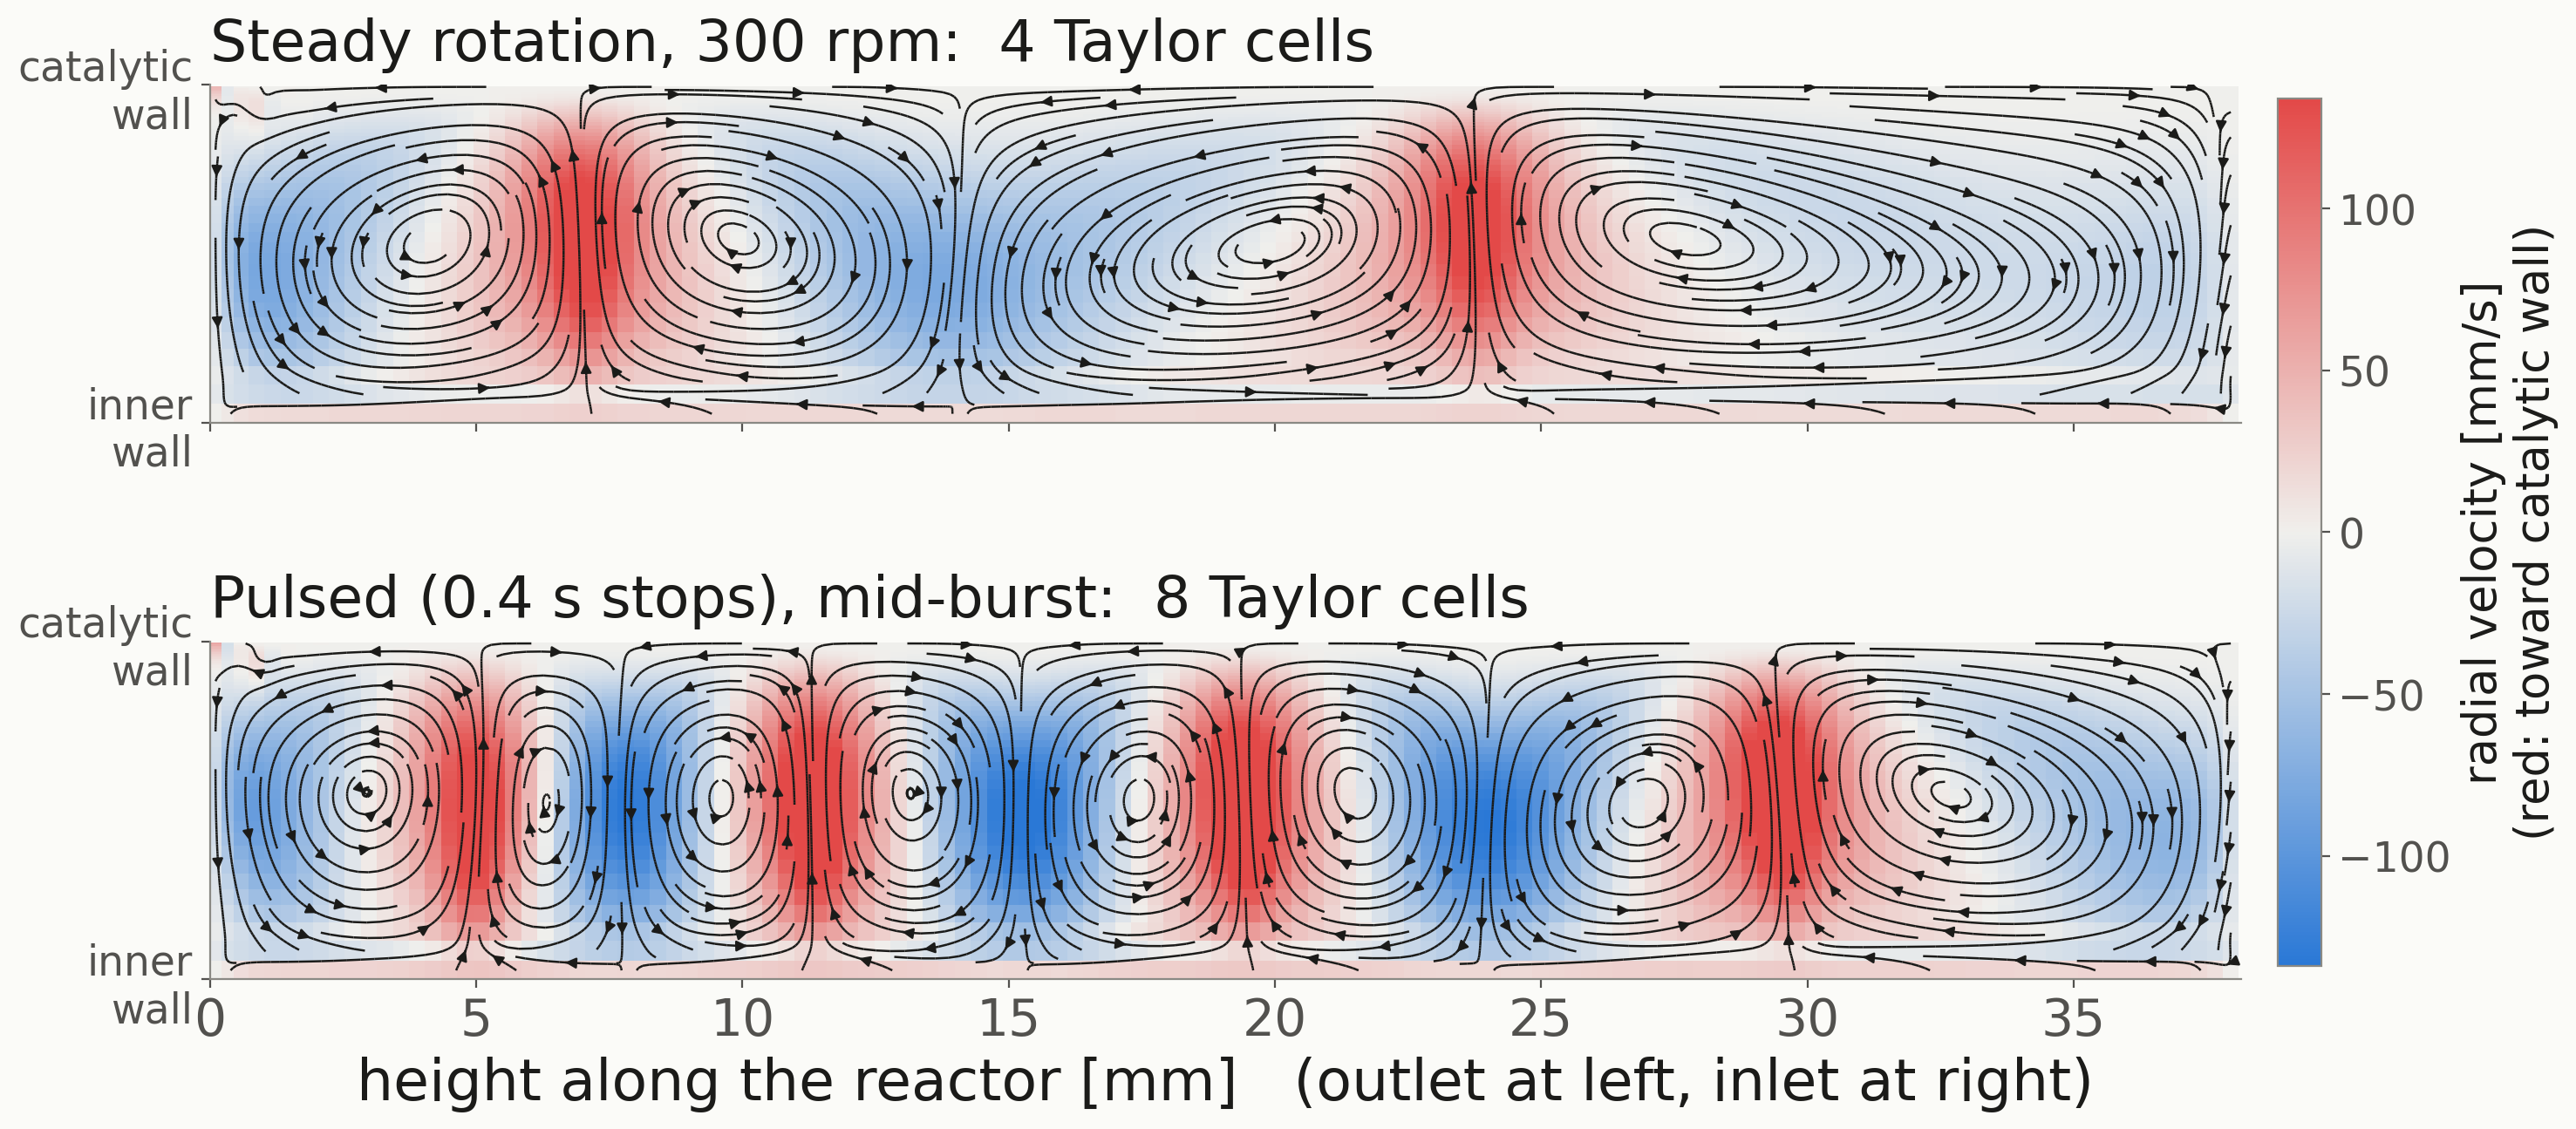
\includegraphics[width=\linewidth,height=0.86\textheight,keepaspectratio]{s_cells_snapshot}
\end{frame}
\note{[1:00] So why does a brief stop help? Both panels show the gap between the cylinders, unrolled sideways: inner wall at the bottom, catalytic wall at the top. Colour is radial velocity; red means liquid heading toward the catalytic wall. Under steady rotation there are four large vortex cells. Under pulsing, mid-burst, there are eight narrower ones. In dynamical-systems language this is multistability: at the same Reynolds number a short Taylor--Couette annulus has several stable solutions with different numbers of cells, and which one you land in depends on the initial condition; Benjamin and Mullin studied this in the early 1980s (check citation). Each brief stop brings the flow nearly to rest, and the restart from rest selects a higher axial wavenumber, eight cells instead of four. Narrower cells carry reactant to the wall faster.}

% ============================================================================
\begin{frame}{Restarts make the extra cells; steady rotation erases them}
  \begin{columns}[T]
    \begin{column}{0.49\textwidth}
      \centering{\small\textbf{Each cycle:} 8 cells, +15\% wall reaction}\par\smallskip
      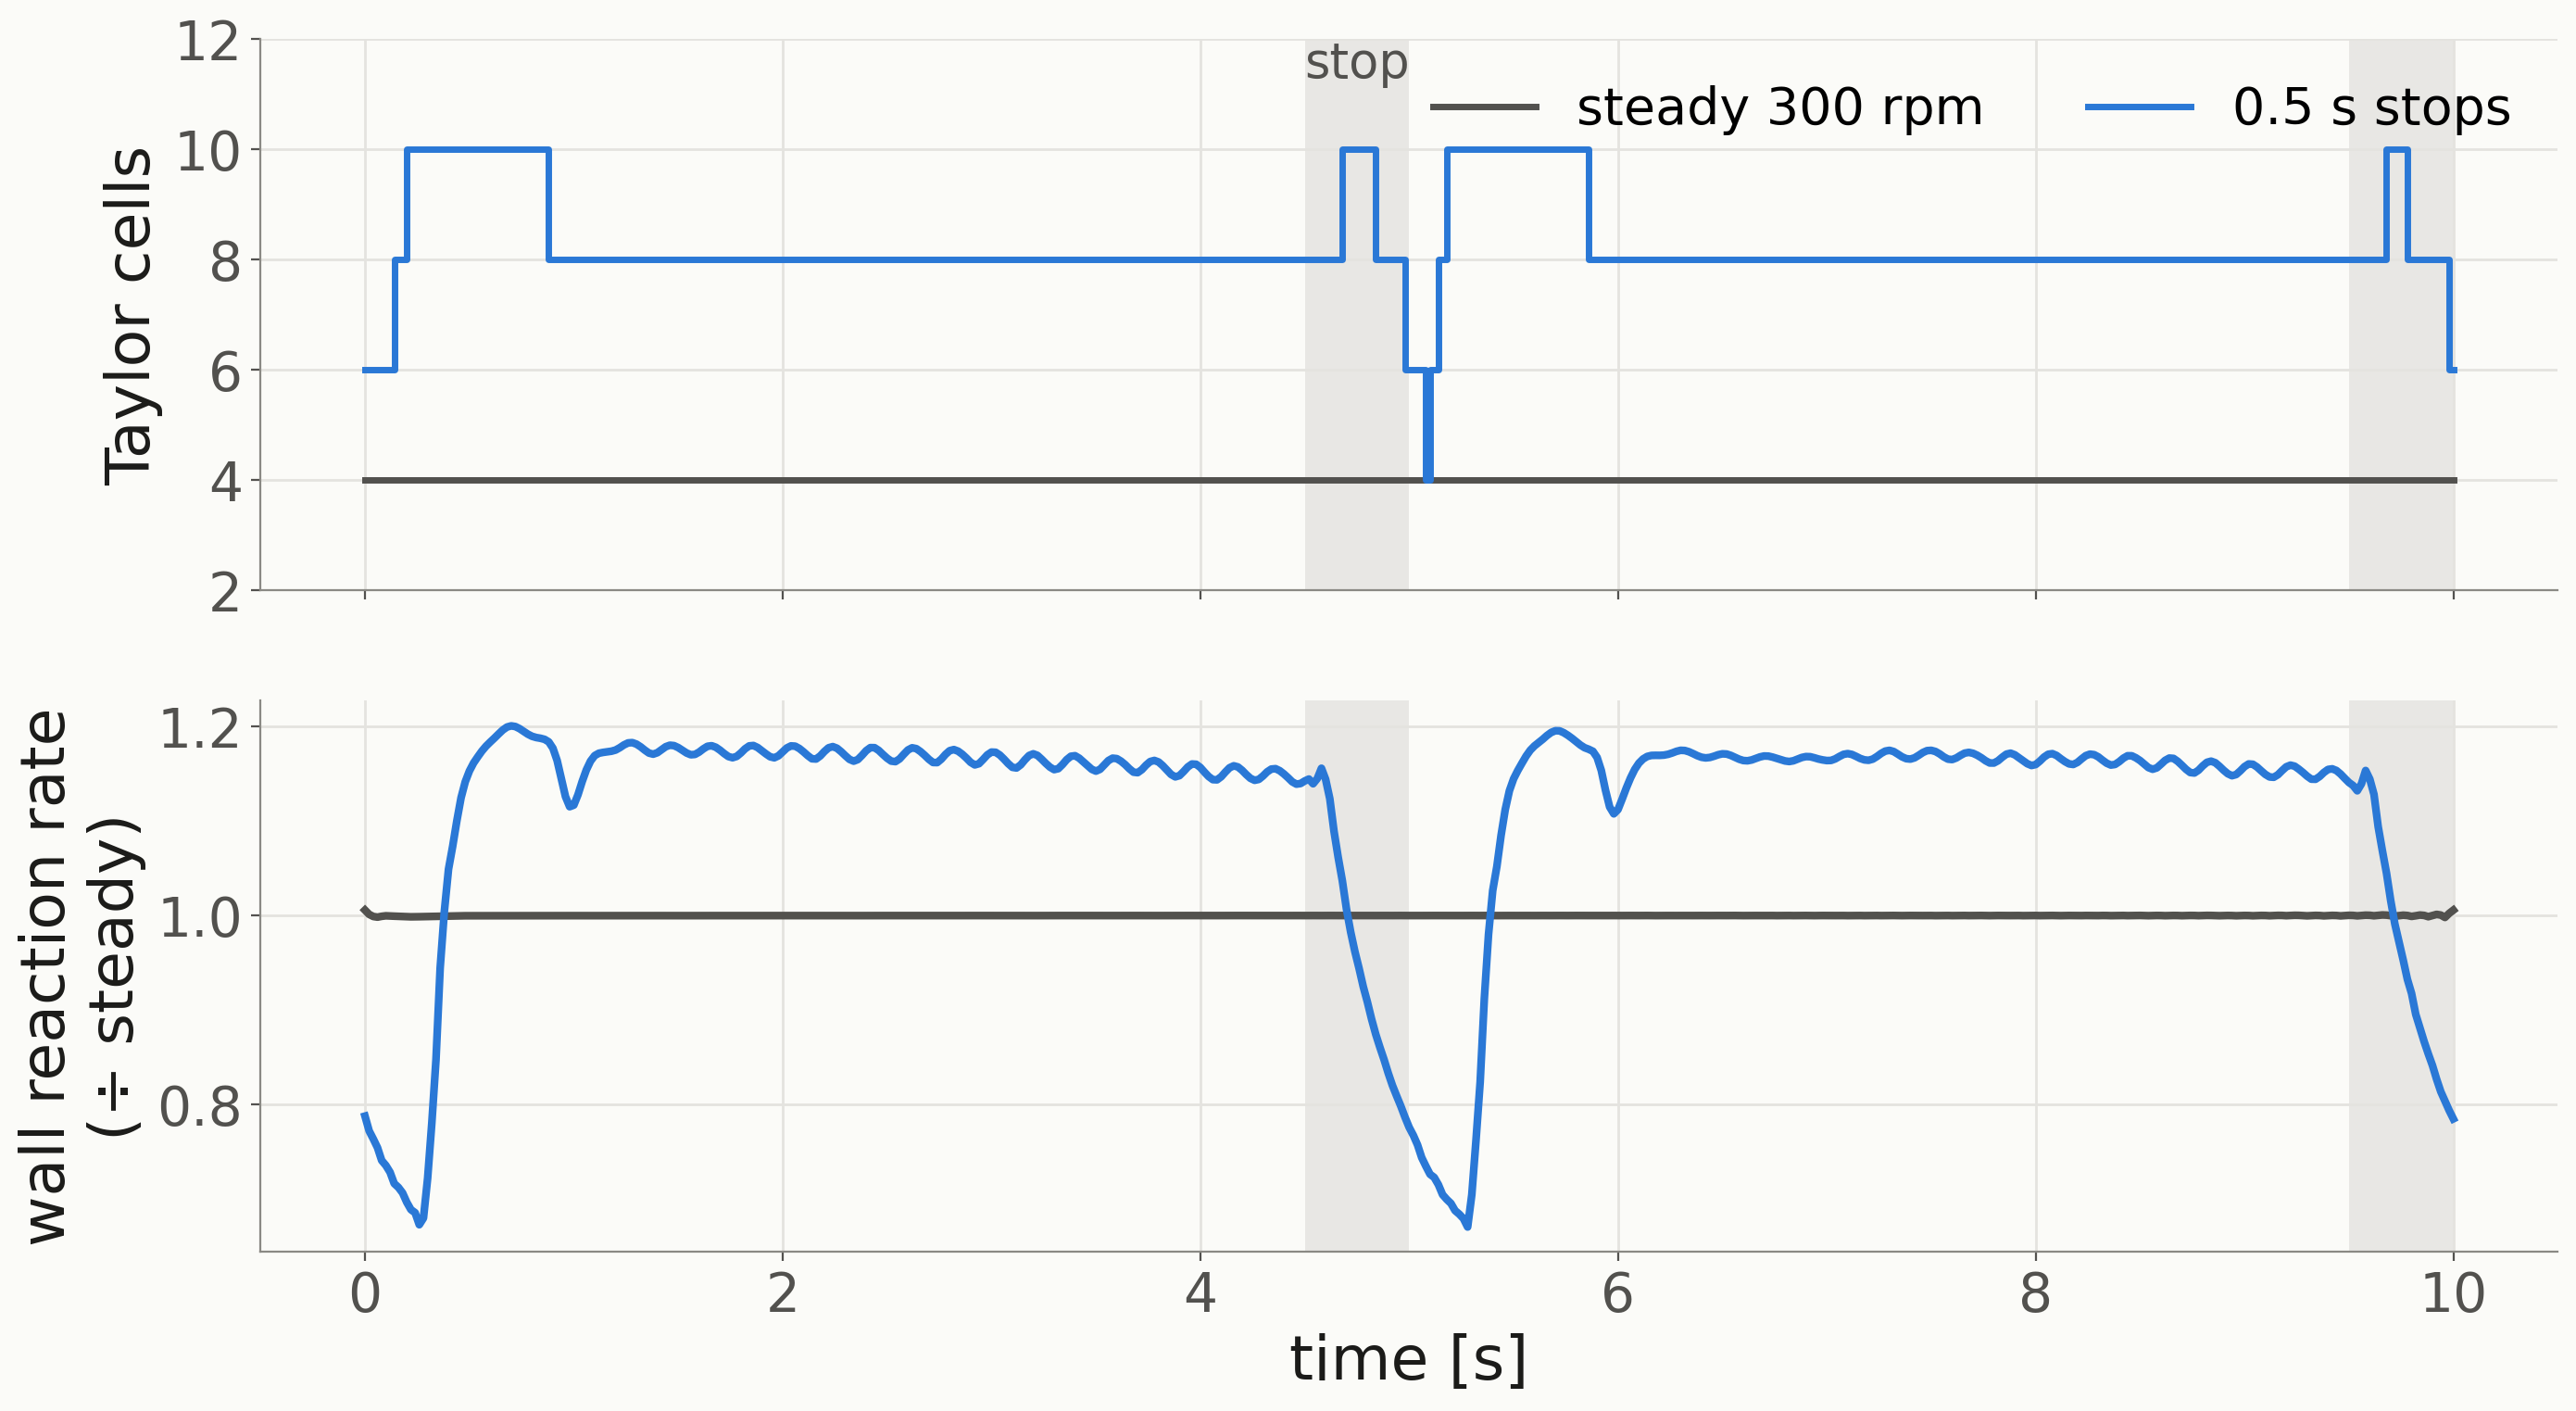
\includegraphics[width=\linewidth,height=0.56\textheight,keepaspectratio]{s_one_cycle}
    \end{column}
    \begin{column}{0.49\textwidth}
      \centering{\small\textbf{Stop pulsing:} back to 4 cells in 10--15\,s}\par\smallskip
      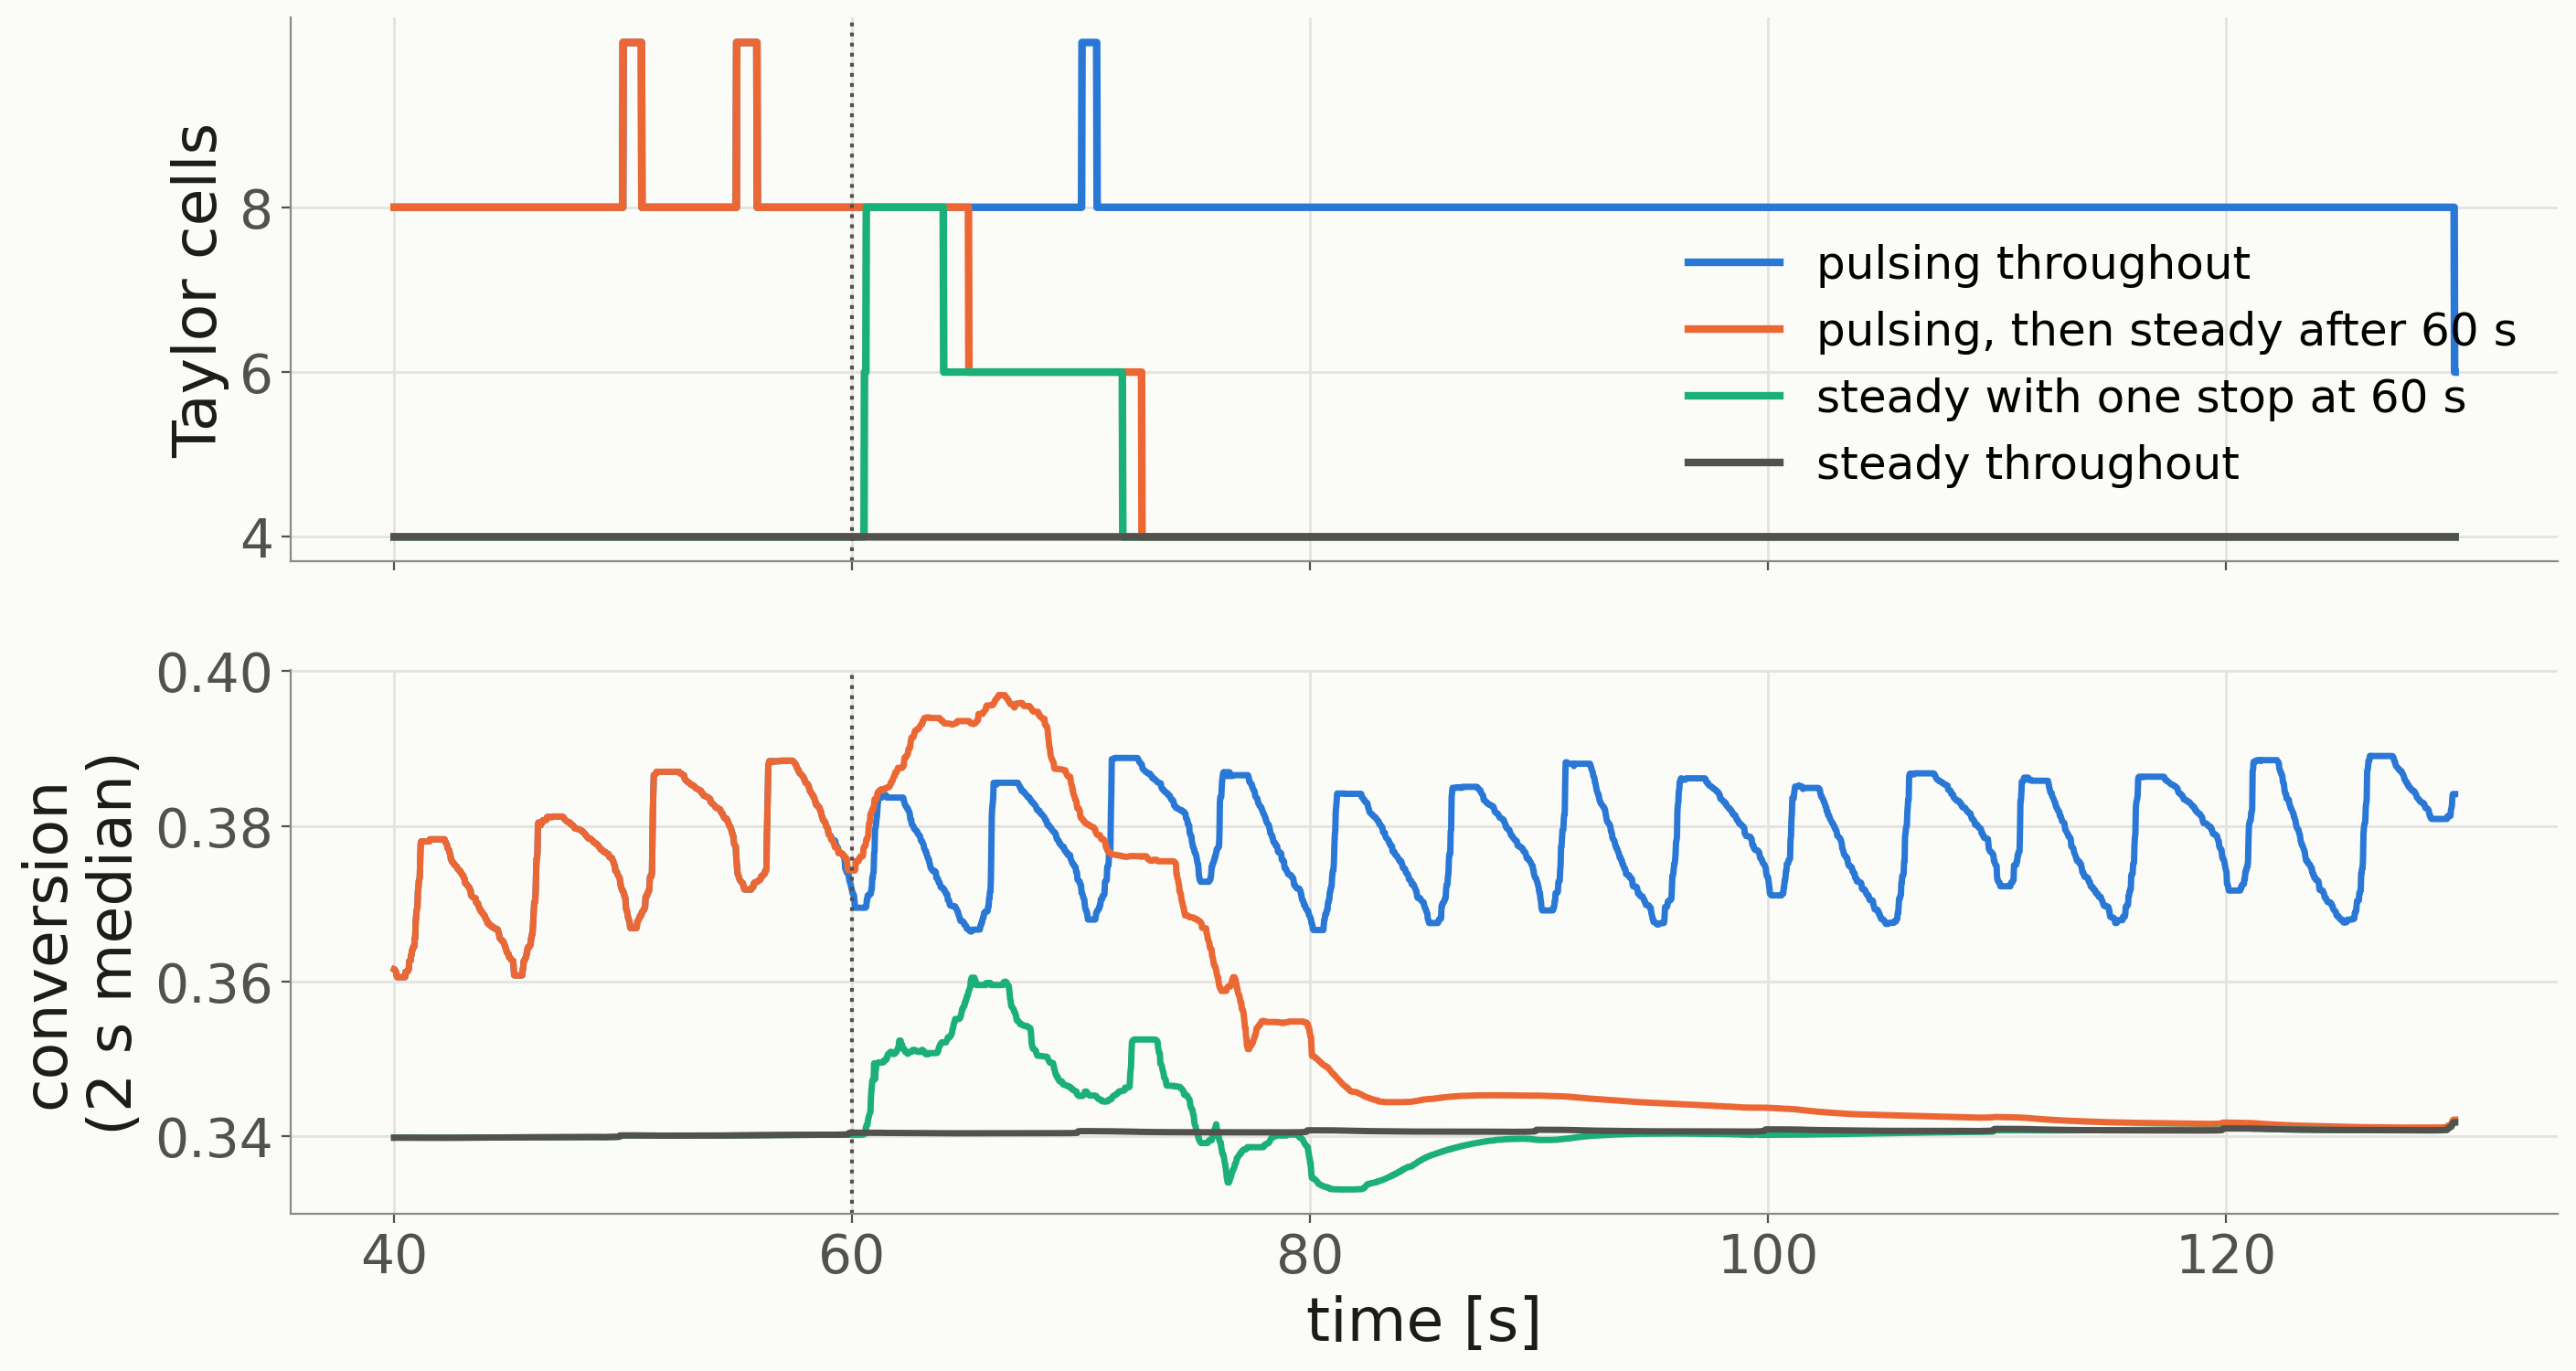
\includegraphics[width=\linewidth,height=0.56\textheight,keepaspectratio]{s_hold_kick}
    \end{column}
  \end{columns}
  \medskip
  \centering\alert{\textbf{Stops must repeat.}}
\end{frame}
\note{[1:00] Inside each cycle: after every restart the cell count jumps up and settles at eight, and the reaction rate at the wall stays about fifteen percent above steady rotation for the whole burst. It isn't a brief spike after the restart; the restart spike contributes almost nothing. On the right: if I pulse until 60 seconds and then hold steady, or do just one stop, the extra cells merge back to four within ten to fifteen seconds, and conversion drops back to the steady value. So the stops have to keep coming every few seconds, which explains why five-second cycles win and the published thirty-second cycle loses.}

% ============================================================================
\begin{frame}{It has to be a full stop}
  \begin{columns}[c]
    \begin{column}{0.68\textwidth}
      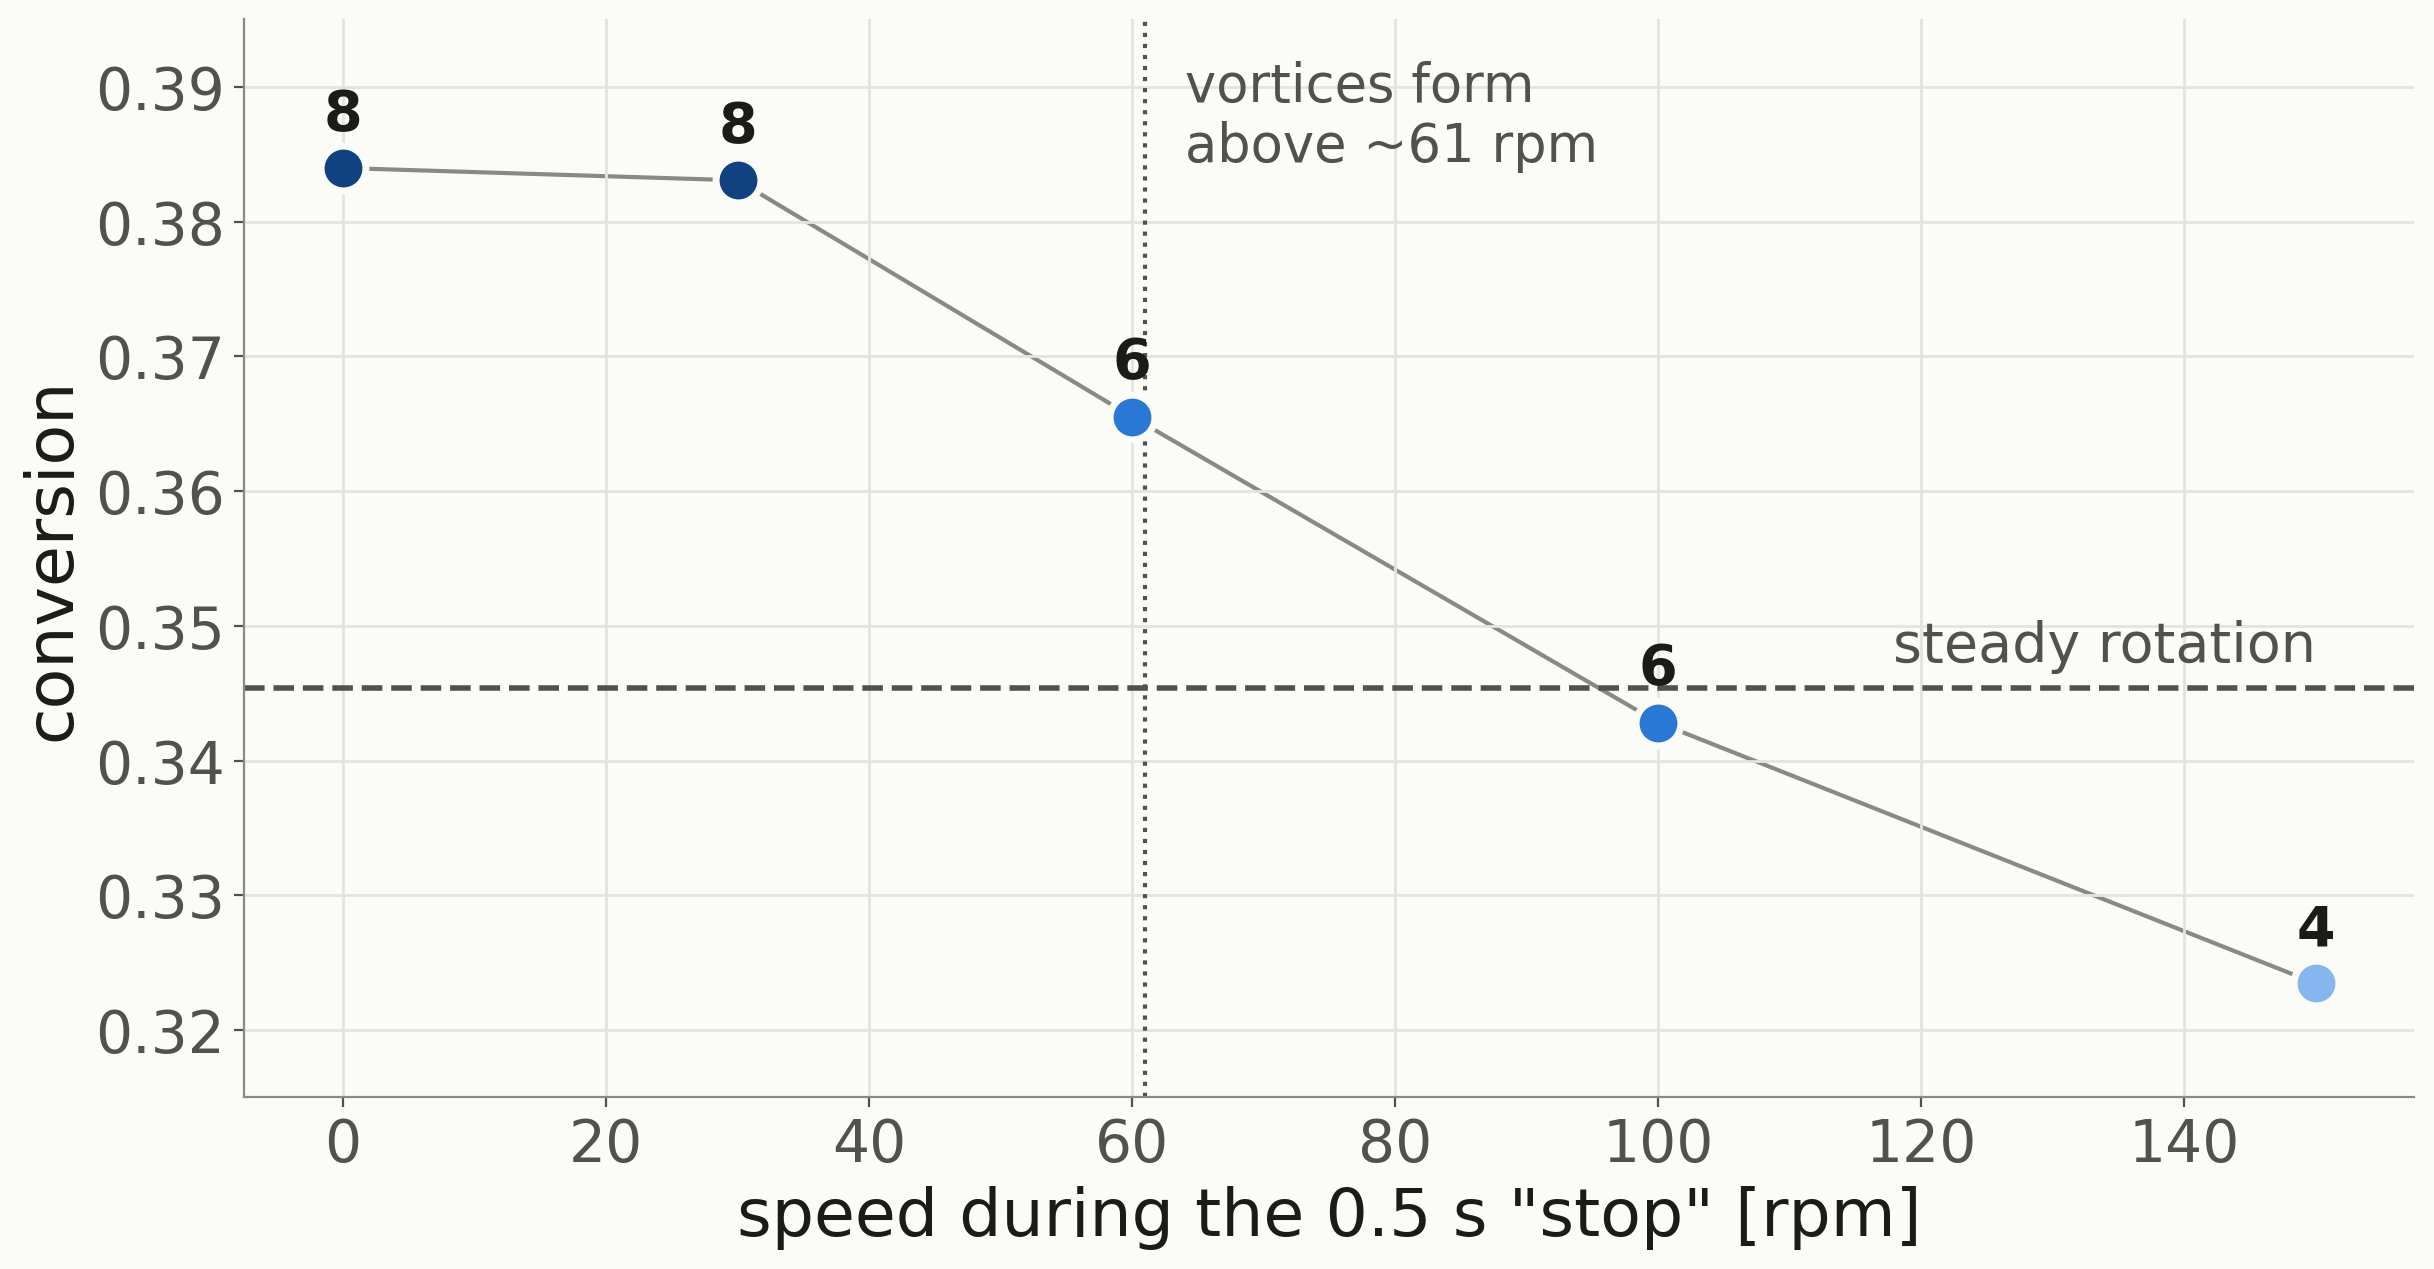
\includegraphics[width=\linewidth,height=0.76\textheight,keepaspectratio]{s_stop_level}
    \end{column}
    \begin{column}{0.30\textwidth}
      Vortices must die first.
    \end{column}
  \end{columns}
\end{frame}
\note{[0:30] Instead of stopping, I slowed the cylinder to 30, 60, 100 or 150 rpm for the same half second. Thirty is as good as a full stop. At 60 rpm, about where vortices start to form, you get six cells instead of eight, and at 100 and above the gain is gone. The vortices really have to die, to about one percent of their energy, before the restart can build a new, finer pattern.}

% ============================================================================
\begin{frame}{Conversion follows the cell count}
  \begin{columns}[c]
    \begin{column}{0.74\textwidth}
      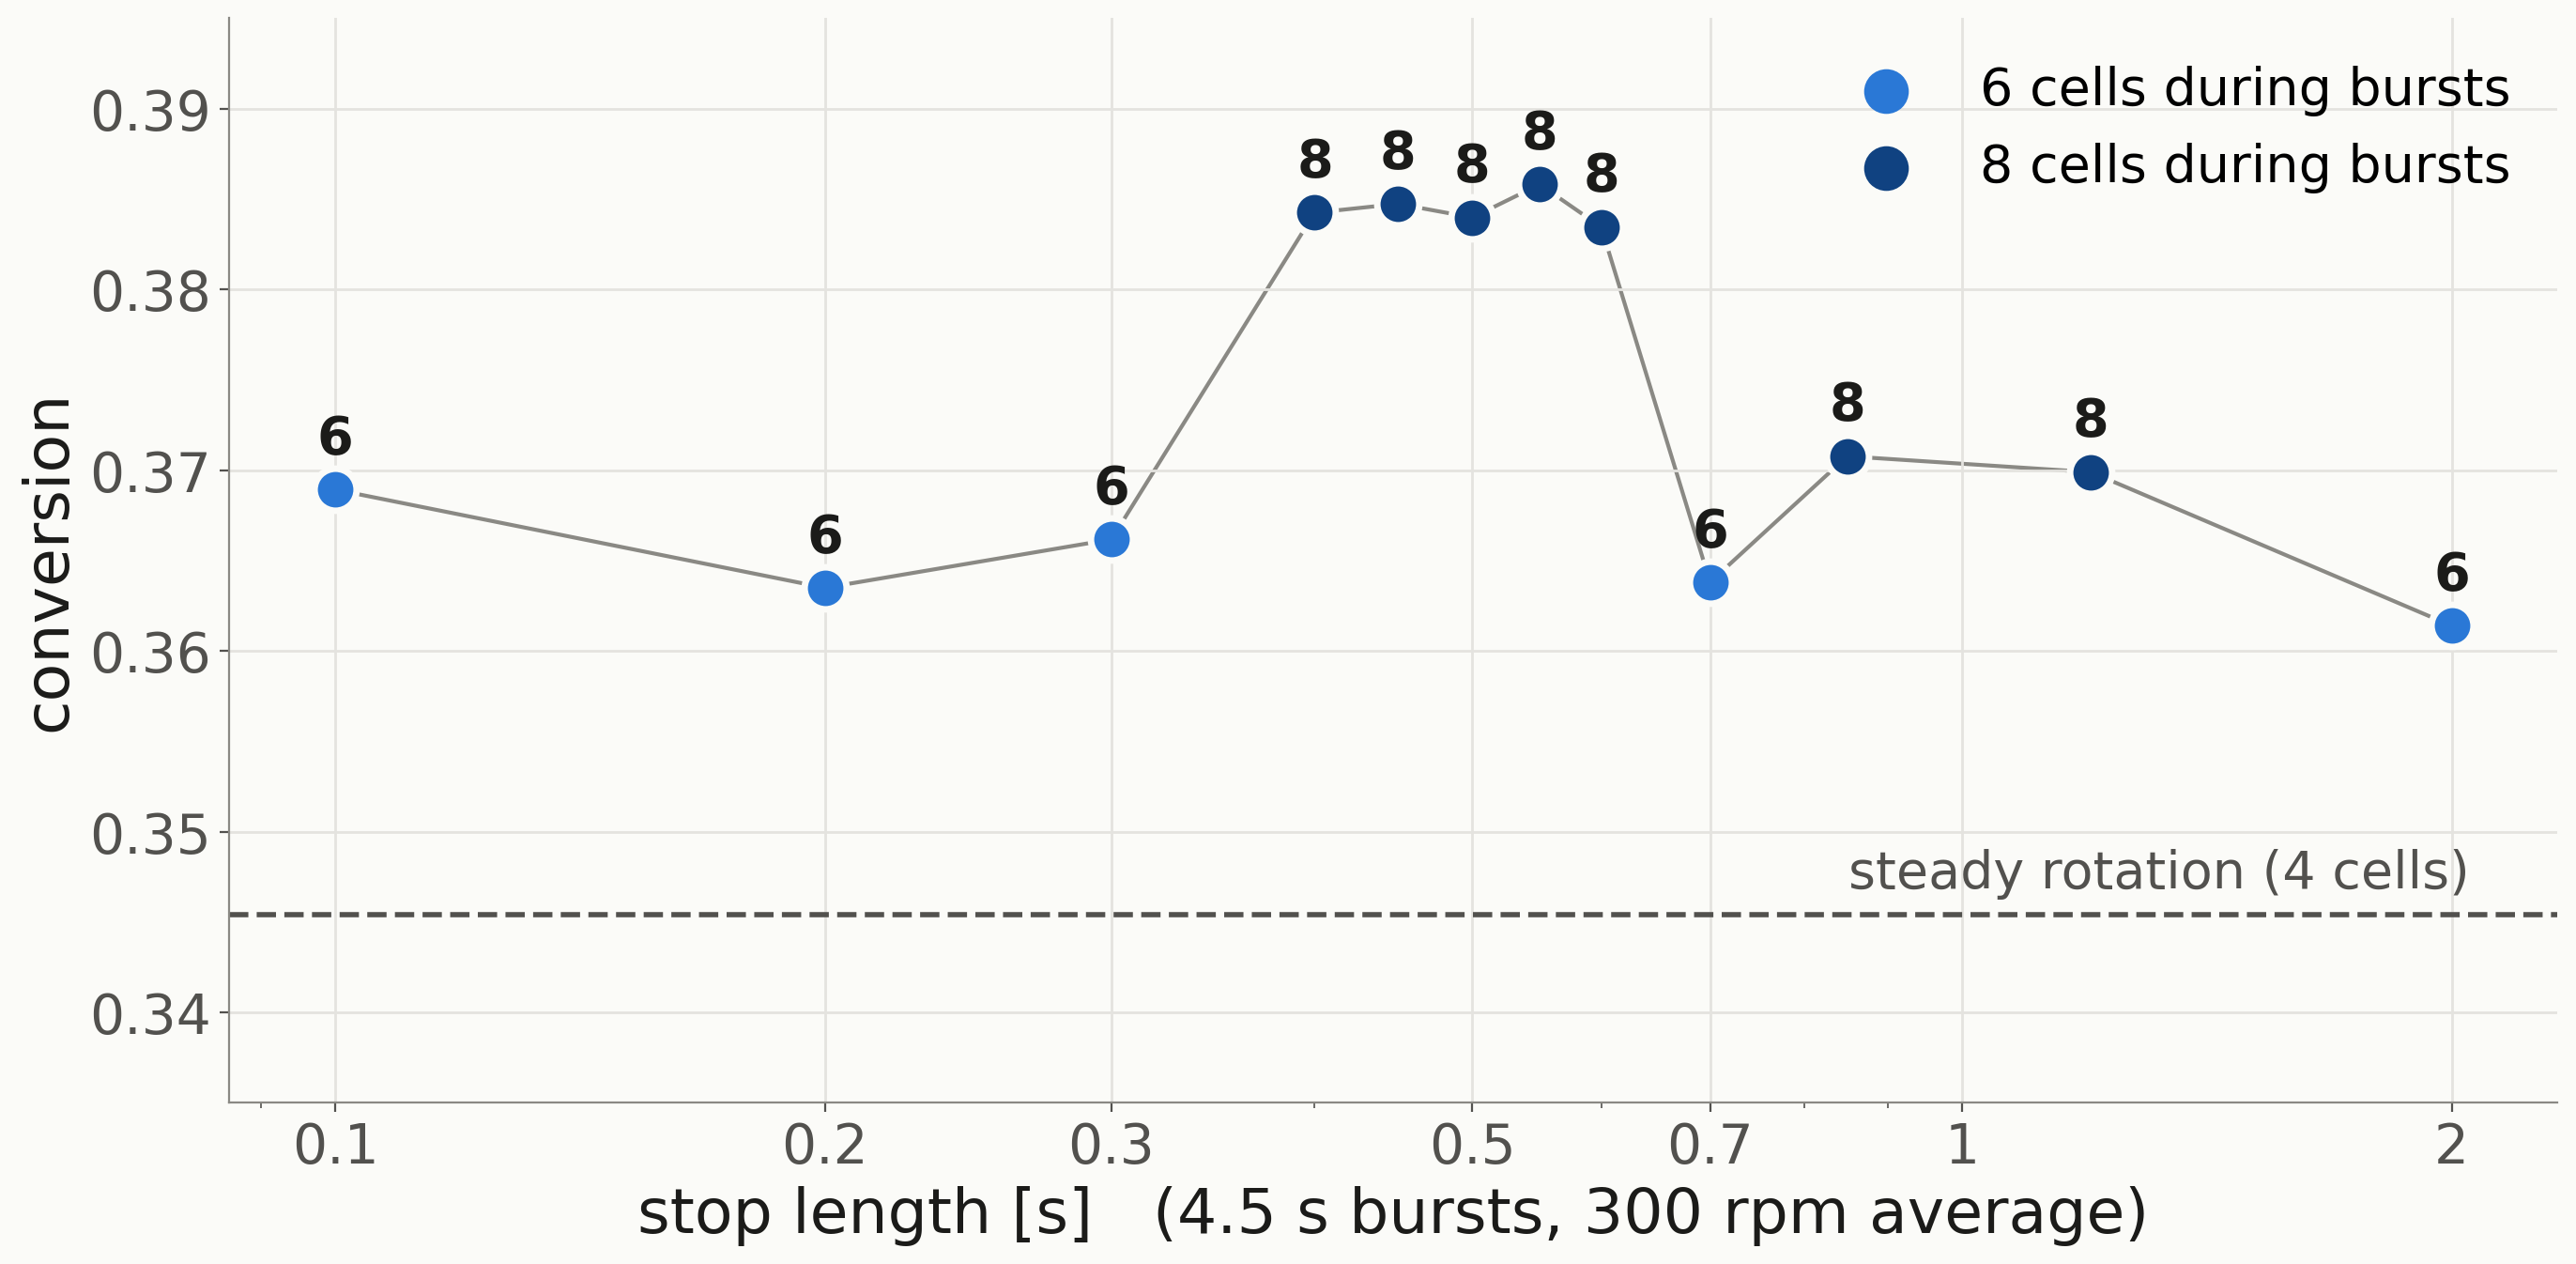
\includegraphics[width=\linewidth,height=0.74\textheight,keepaspectratio]{s_stop_curve_cells}
    \end{column}
    \begin{column}{0.24\textwidth}
      \bignum{+0.04}{conversion in the 8-cell window (0.4--0.6\,s stops)}\par\bigskip
      \bignum{4\,$\to$\,8}{cells, steady vs best pulsing}
    \end{column}
  \end{columns}
\end{frame}
\note{[0:45] Plot conversion against stop length and label each point with its cell count. It isn't a smooth curve with one peak; it's a set of levels. Steady rotation, four cells, at the bottom; six-cell stops in the middle; and the best stops, 0.4 to 0.6 seconds, are exactly the ones whose restart lands in eight cells, about 0.04 above steady rotation. The sudden drop at 0.7 seconds, which looked like a strange cliff in the original search, is just the flow falling back to six cells.}

% ============================================================================
\begin{frame}{Numerical verification}
  \begin{columns}[T]
    \begin{column}{0.58\textwidth}
      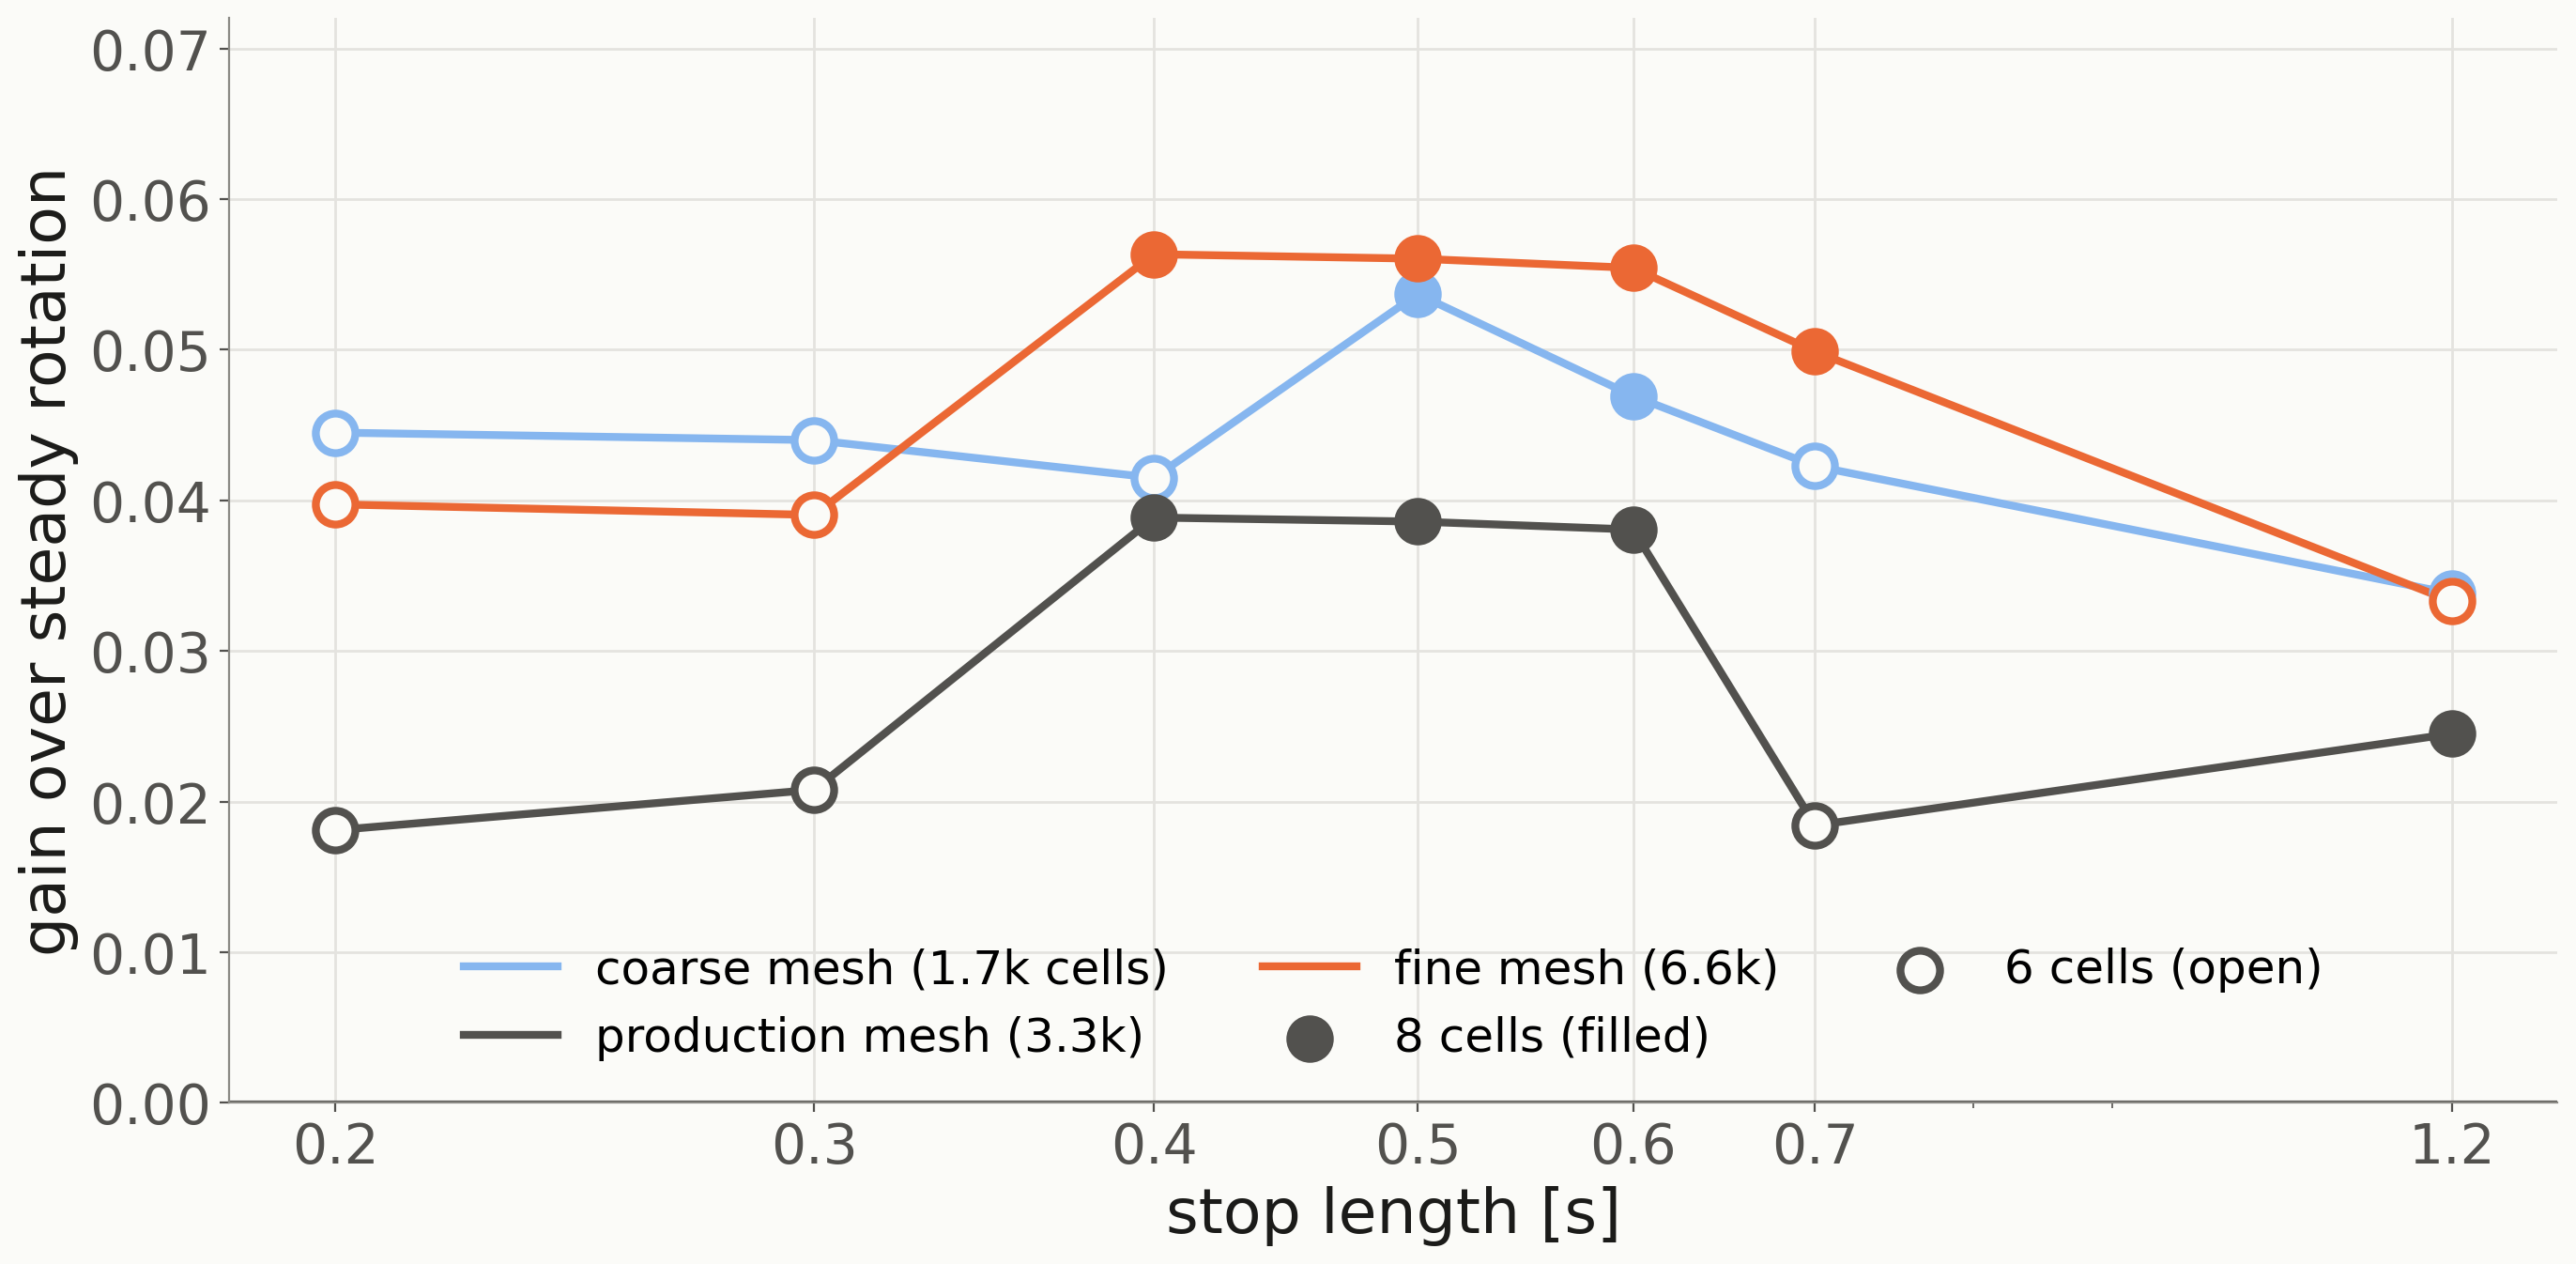
\includegraphics[width=\linewidth,height=0.62\textheight,keepaspectratio]{s_mesh_check}\par
      {\small\color{ink}3 meshes: same cells, gain +0.04 to +0.06}
    \end{column}
    \begin{column}{0.40\textwidth}
      \begin{block}{Checks}
        \begin{itemize}
          \item Half time step: outlet artifact gone
          \item Mass balance: 0.3\%
          \item Replicate noise: 0.002
        \end{itemize}
      \end{block}
    \end{column}
  \end{columns}
\end{frame}
\note{[0:45] For this audience the obvious question is whether it's numerics. I repeated the key runs on a coarser and a finer mesh from the same self-similar family. On all three, steady rotation has four cells, the best stops land in eight, and the gain is four to six hundredths. Halving the time step exposed and removed a spurious jet at the outlet worth about four hundredths of conversion, which is why all these runs use the smaller step. The mass balance closes to a third of a percent and replicate noise is about 0.002. What does move with the mesh is the exact edges of the eight-cell window, by a tenth of a second or two, so I quote ``about half a second''.}

% ============================================================================
\begin{frame}{Three takeaways}
  \begin{enumerate}
    \setlength\itemsep{0.8em}
    \item Brief full stops beat steady rotation and the published recipe.
    \item RL learns near-optimal control: matches 220-run optimization, transfers $5\times$ taller.
    \item Mechanism: restarts select more Taylor cells (8 vs 4); stops must repeat.
  \end{enumerate}
  \vfill
  {\small\color{ink}\textbf{Next:} messy conditions (feed, fluid drift) $\to$ feedback control; 3D check.\par\smallskip
  \textbf{Limits:} 2D axisymmetric; $\mathrm{Sc}=1075$.}
\end{frame}
\note{[0:45] One: brief full stops beat steady rotation at the same power, and beat the published recipe. Two: the RL pipeline learns near-optimal control from simulation alone. With no physics given, it matched an independent 220-run optimization, which is how we know it found the right answer, and it carried over to a reactor five times taller. Three: the optimum exploits multistability. Each restart selects a state with more cells that transports reactant faster, and because that state decays back under steady forcing, the stops have to repeat. This problem turned out to be simple: steady conditions, one best waveform, so a static optimizer can solve it too, and RL tying it is what you'd expect. The next step is to make it messy: changing feed rates and drifting fluid properties, where no fixed waveform stays right and a feedback policy should pull ahead. The main limit is the 2D model, so the mechanism is still a hypothesis for real 3D flow. Thank you, happy to take questions.}

% ============================================================================
\appendix
\begin{frame}{Backup: best fixed waveform vs the RL policy}
  \centering
  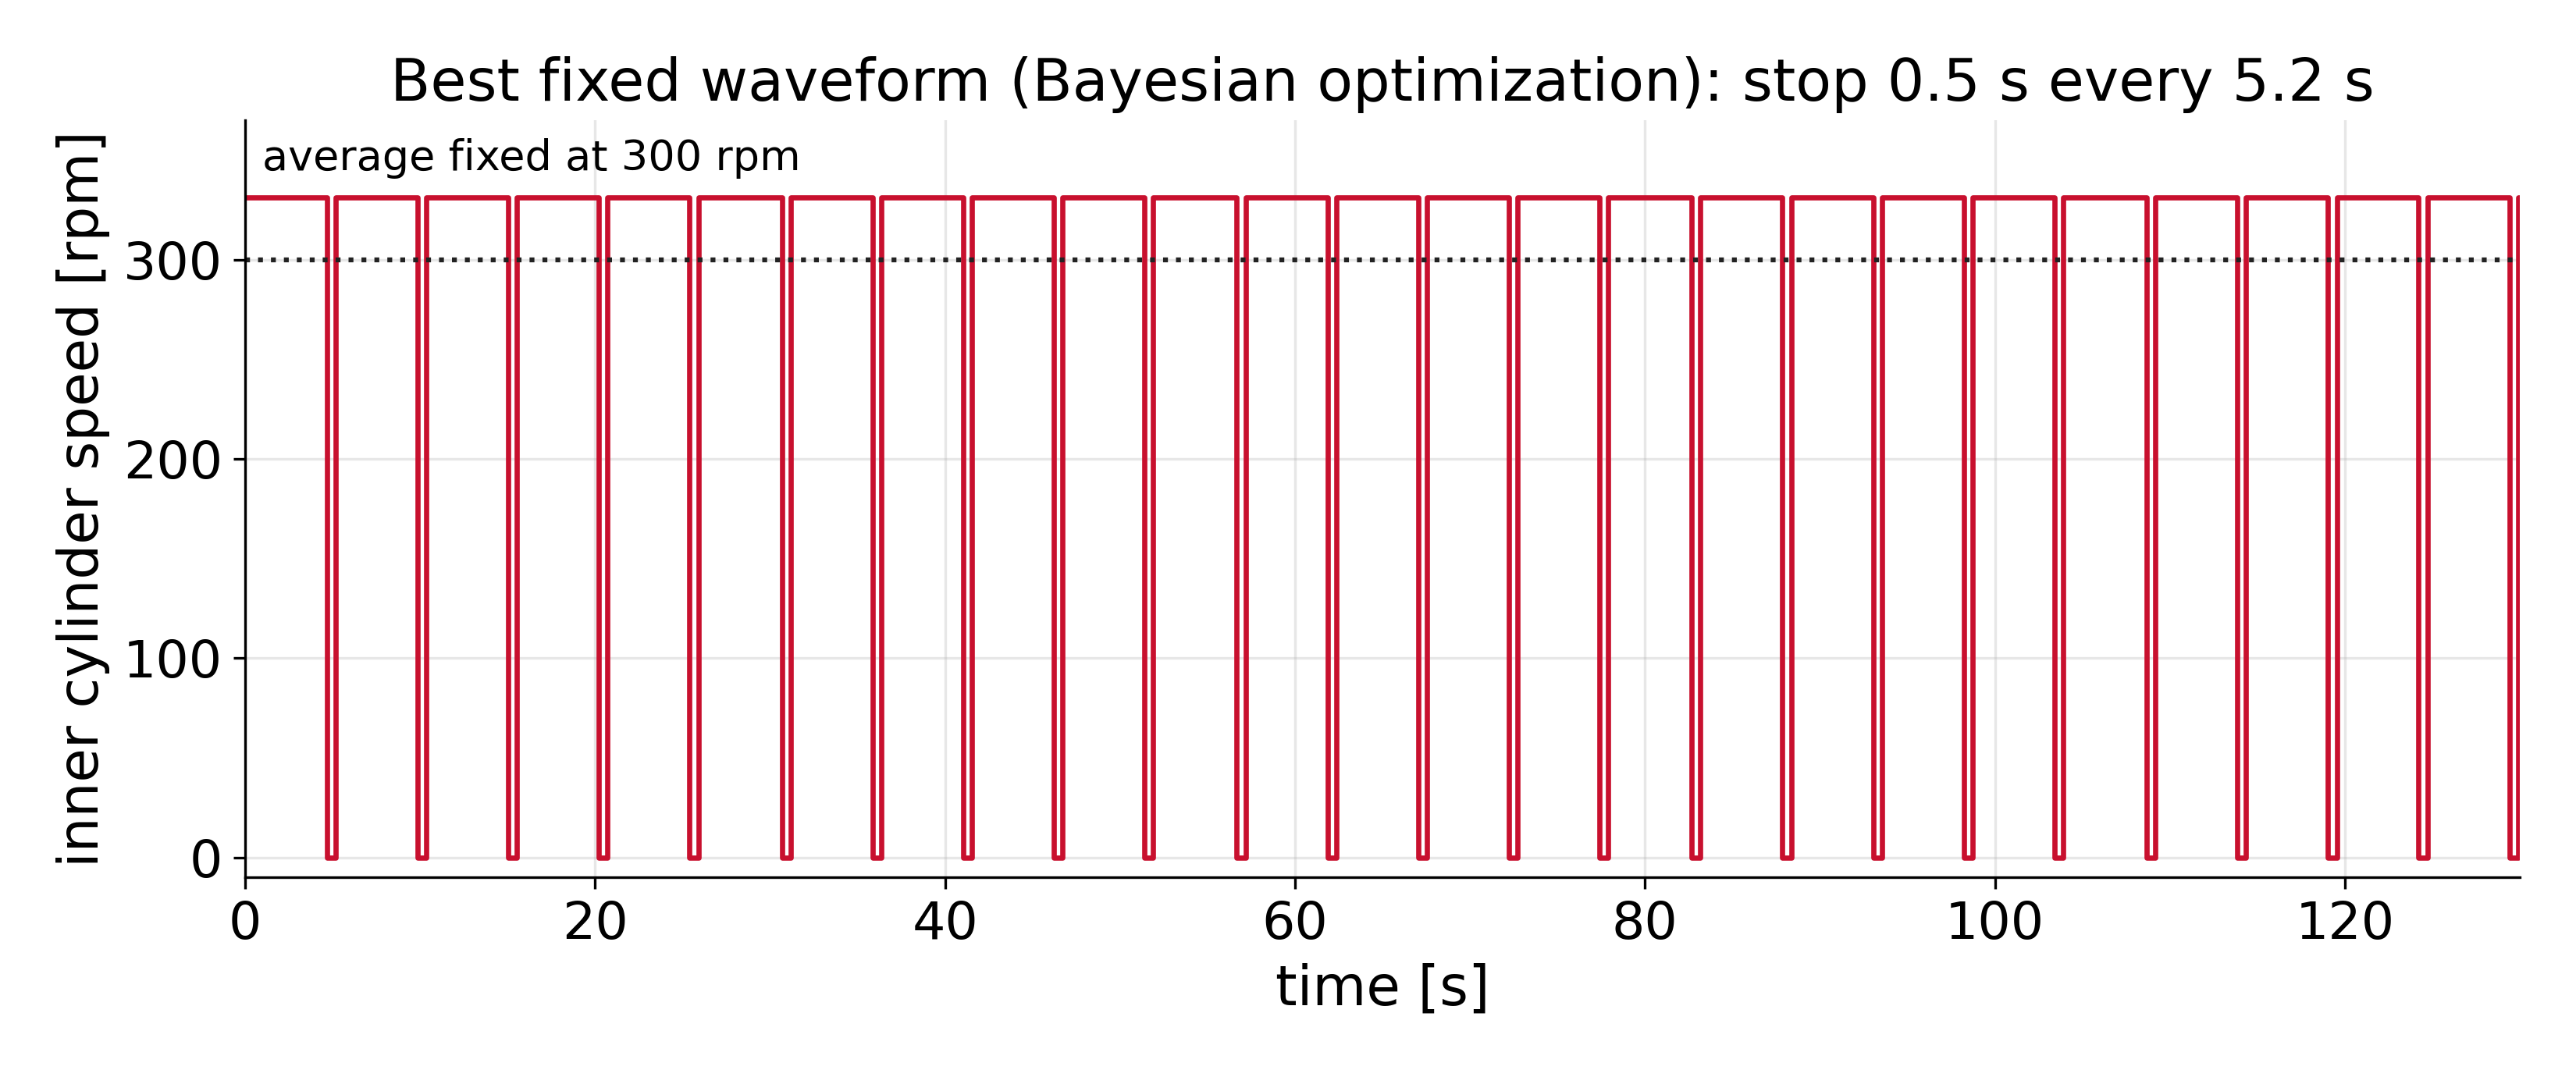
\includegraphics[width=0.86\linewidth,height=0.40\textheight,keepaspectratio]{bo_best_waveform}\par\smallskip
  \includegraphics[width=0.86\linewidth,height=0.40\textheight,keepaspectratio]{fig4_learned_waveform}
\end{frame}
\note{[Backup] Top: the best fixed waveform from the 220-run Bayesian optimization, stop half a second every five seconds, peak about 330 rpm. Bottom: what the RL policy chose. Same idea, brief full stops at high duty, but RL's stops are shorter, mostly a tenth to four tenths of a second, which mostly lands in the six-cell state and costs it one to two hundredths of conversion.}

% ============================================================================
\begin{frame}{Backup: why 0.5\,s? Two time scales, two predictions}
  \begin{columns}[T]
    \begin{column}{0.48\textwidth}
      \begin{block}{Swirl decay}
        \[ \tau = \frac{d^2}{\pi^2 \nu} \approx 0.4\ \mathrm{s} \]
        Slowest decay mode of momentum diffusion across the gap. Predicts best stop $\propto \nu^{-1}$.
      \end{block}
    \end{column}
    \begin{column}{0.48\textwidth}
      \begin{block}{Wall layer}
        \[ \tau = \frac{\delta^2}{D} \approx 0.8\ \mathrm{s} \]
        Regrowth of the depleted layer at the wall. At fixed $D$, predicts best stop $\propto \nu^{0.3}$ to $\nu^{0.7}$.
      \end{block}
    \end{column}
  \end{columns}
  \bigskip
  \takeaway{\textbf{Test:} vary $\nu$ at fixed $D$ and fit best stop $\propto \nu^{a}$. The sign of $a$ decides.}
\end{frame}
\note{[Backup] If asked whether a simple time scale explains the stop length: why half a second? Two time scales sit near it. One is the decay of the swirl: the slowest mode of momentum diffusion across a gap of width d decays on d squared over pi squared nu, about 0.4 seconds. The other is the time for the reactant-depleted layer at the wall to regrow, delta squared over D, about 0.8 seconds. They scale differently with viscosity. Holding the diffusivity fixed, the swirl clock predicts the best stop goes like nu to the minus one; the wall-layer clock predicts a positive power, about 0.3 to 0.7. So I varied the viscosity, fit an exponent, and decided in advance that its sign would pick the winner.}

% ============================================================================
\begin{frame}{Backup: neither guess sets the best stop}
  The swirl decays exactly as theory says (left), but the best stop follows neither prediction (right).\par\medskip
  \centering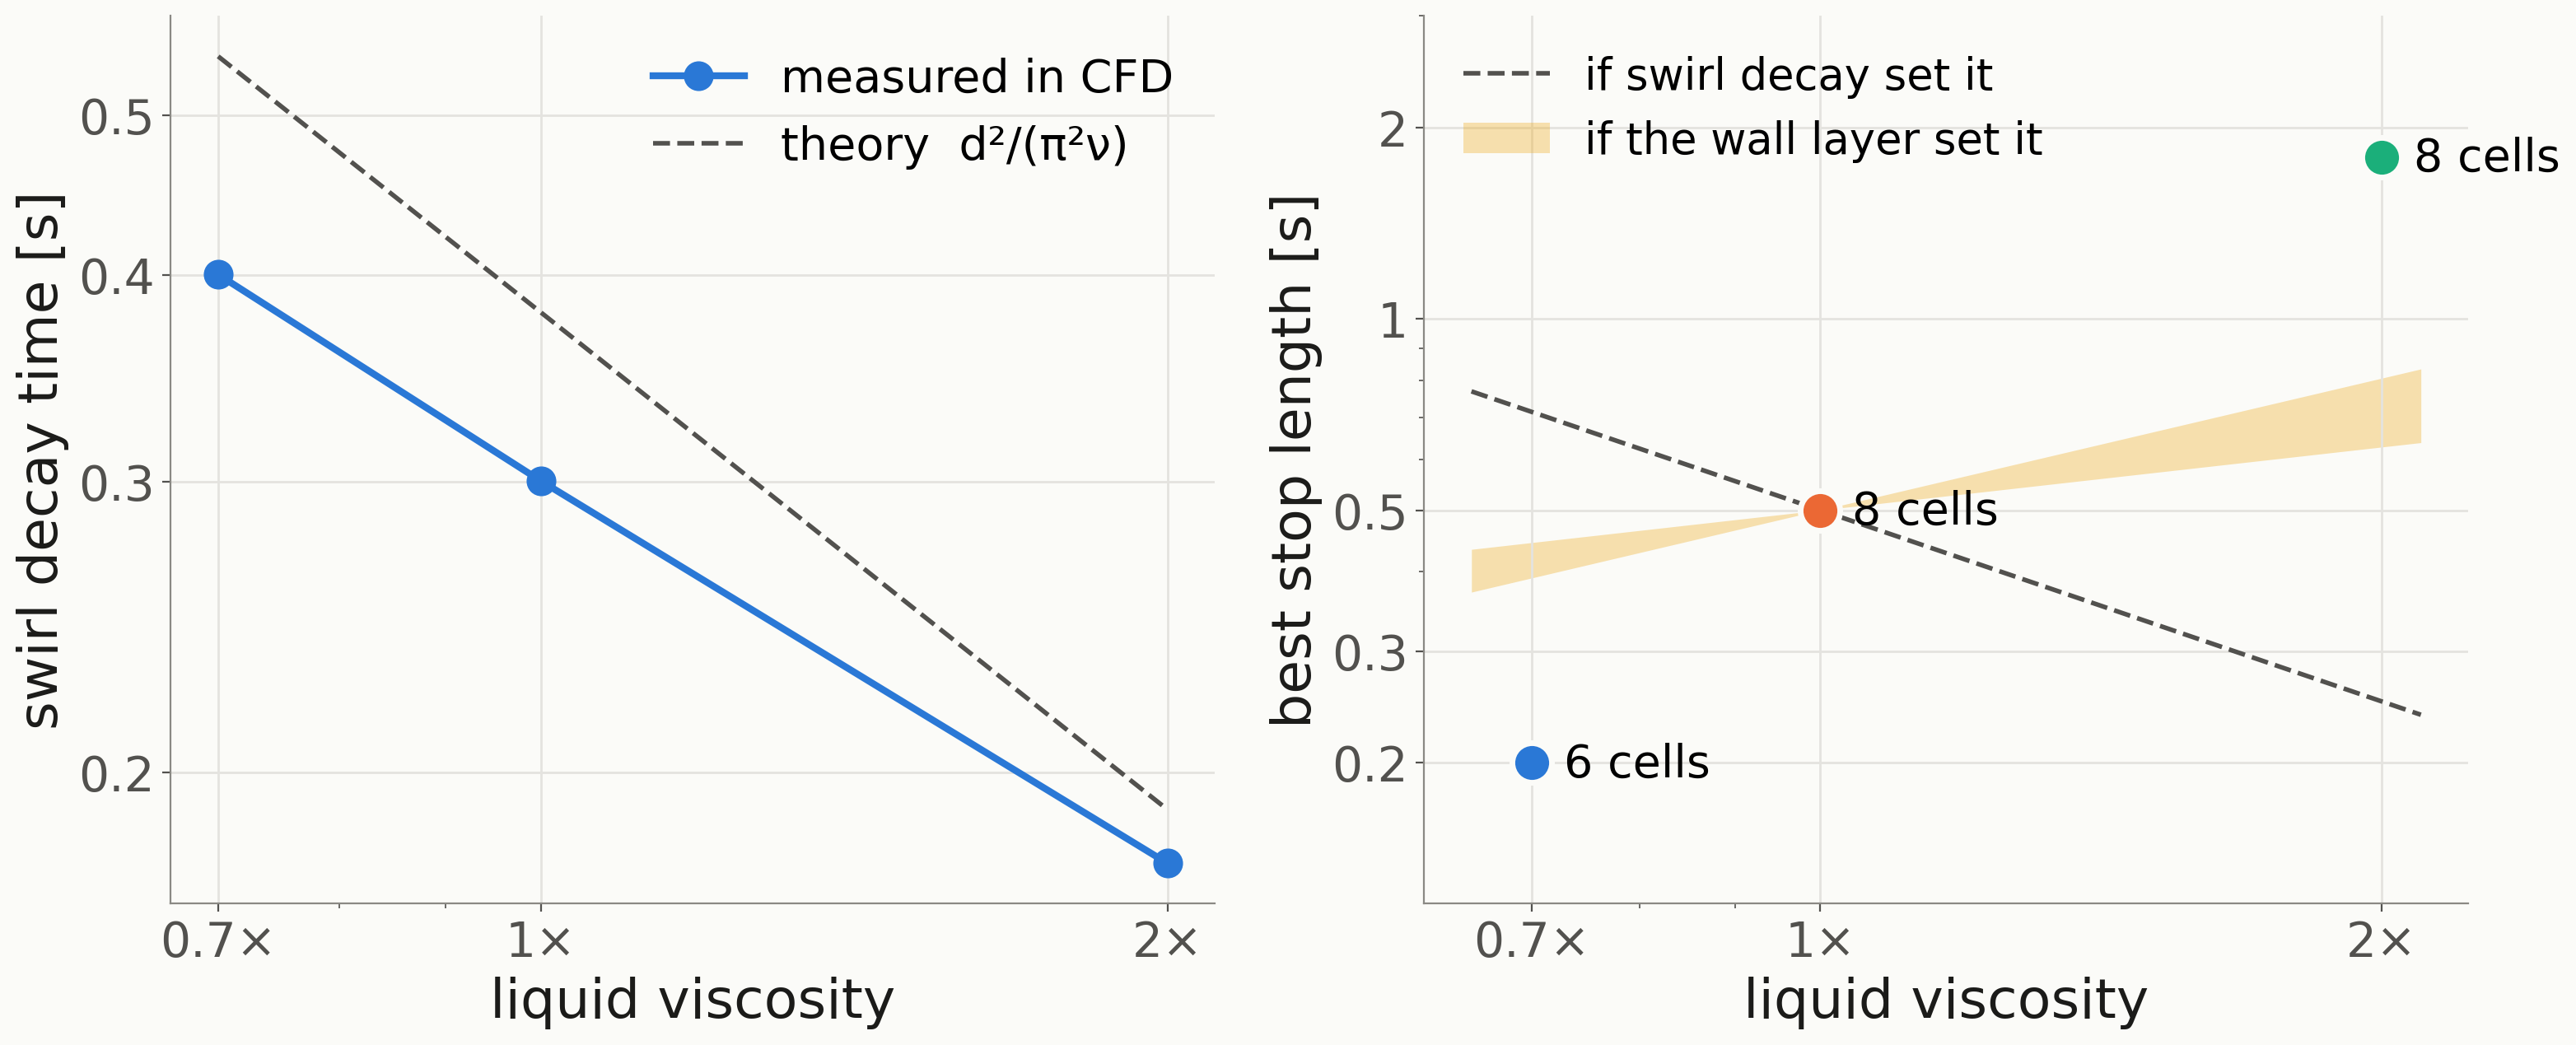
\includegraphics[width=\linewidth,height=0.66\textheight,keepaspectratio]{s_clocks}
\end{frame}
\note{[Backup] On the left, the swirl decays exactly as the eigenmode estimate says, one over viscosity. On the right, the best stop follows neither prediction; a formal exponent fit isn't even meaningful, because the optimum jumps rather than drifting. The labels, six cells and eight cells, are the clue.}


\begin{frame}{Backup: the gain is a higher plateau, not a restart spike}
  \centering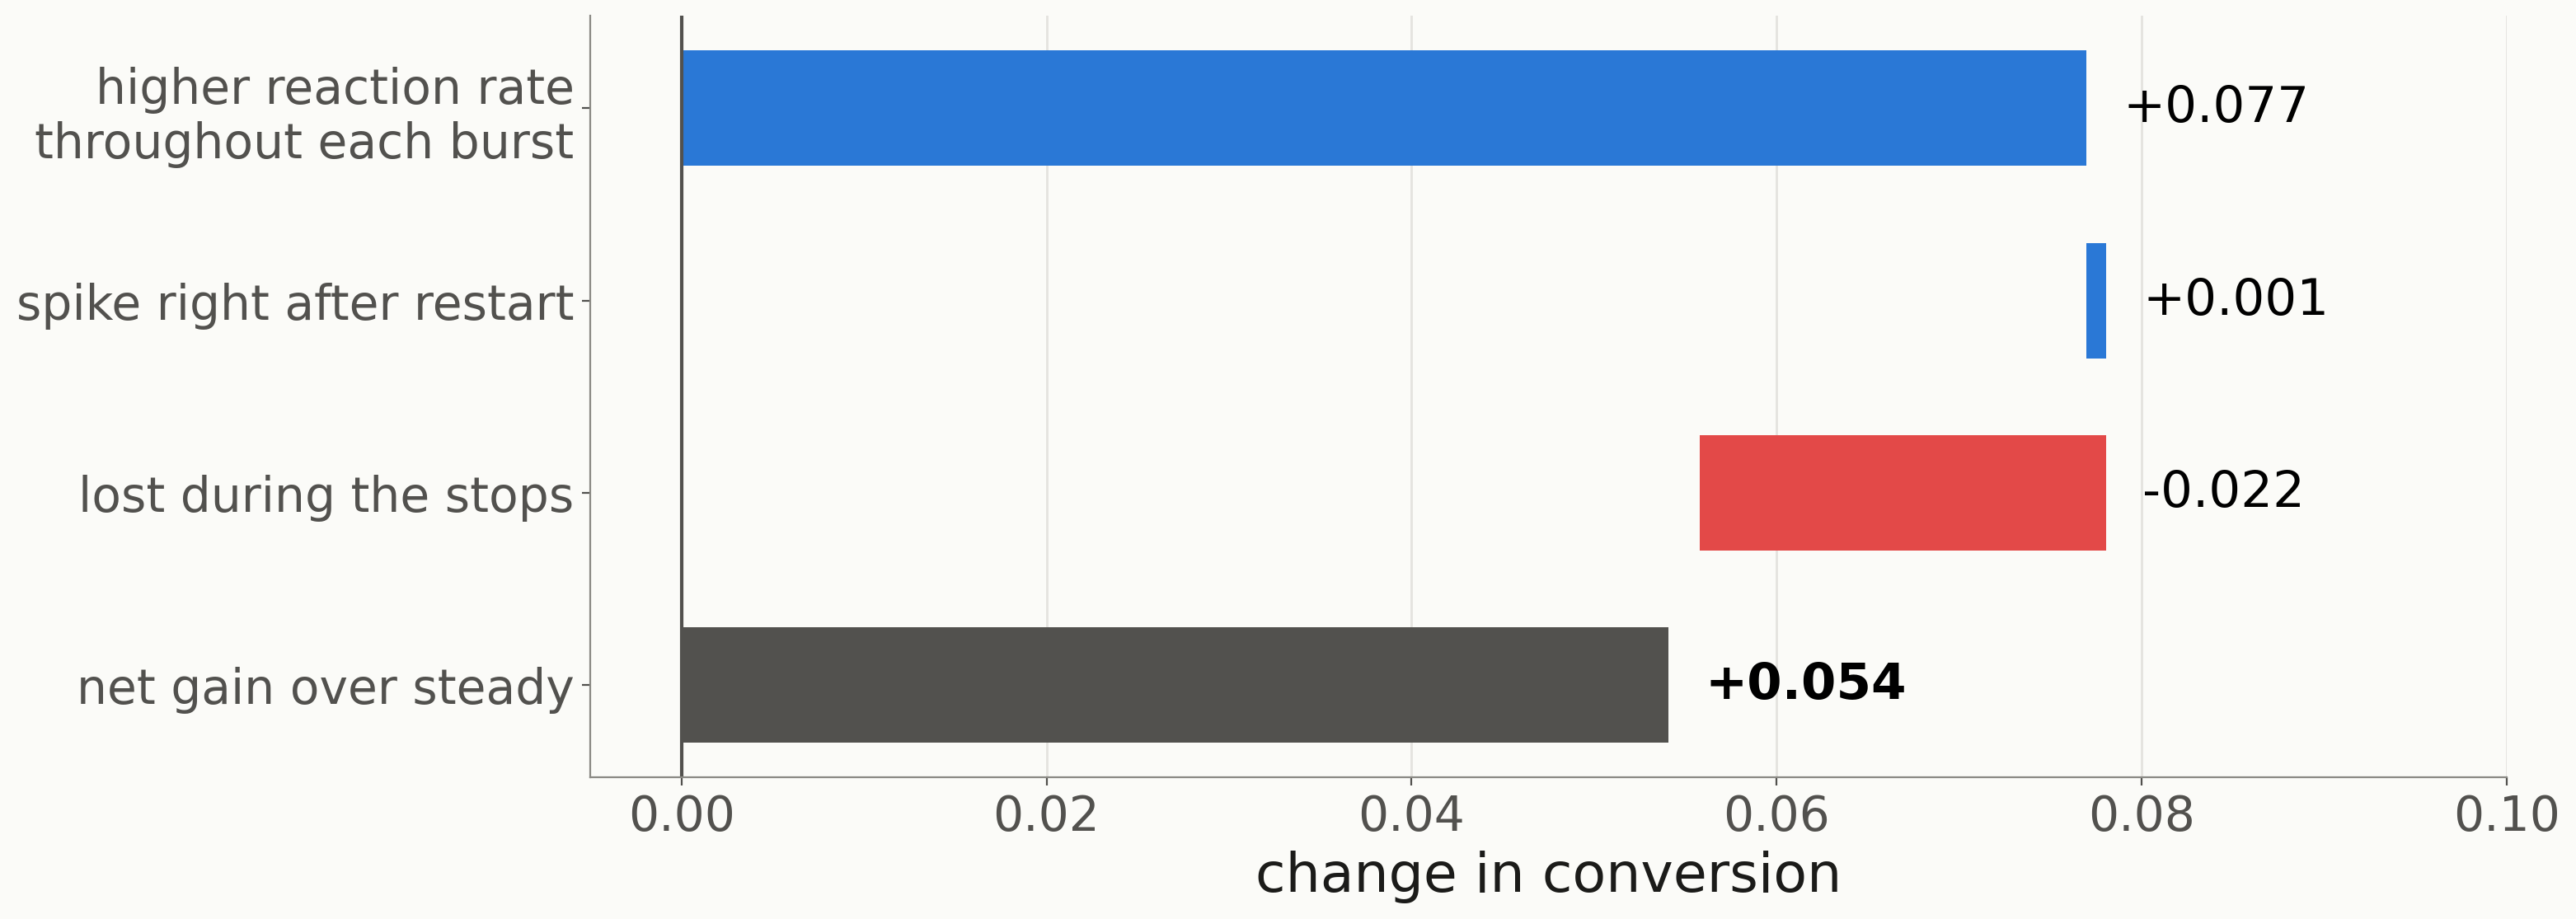
\includegraphics[width=\linewidth,height=0.62\textheight,keepaspectratio]{s_gain_breakdown}\par\smallskip
  \raggedright{\small\color{ink}From the wall-reaction traces of the best waveform's original run (wall-flux budget, last 26\,s).}
\end{frame}
\note{[Backup] If asked whether this is just a restart spike (``film renewal''): no. Splitting the gain over steady rotation: +0.077 from the reaction rate staying higher through the whole burst, only +0.001 from the spike right after restart, and $-0.022$ lost while stopped. The parts sum to 0.056 against the measured 0.054; the difference comes from how the burst plateau is defined.}

\begin{frame}{Backup: gain needs cells added over steady rotation}
  \begin{columns}[c]
    \begin{column}{0.64\textwidth}
      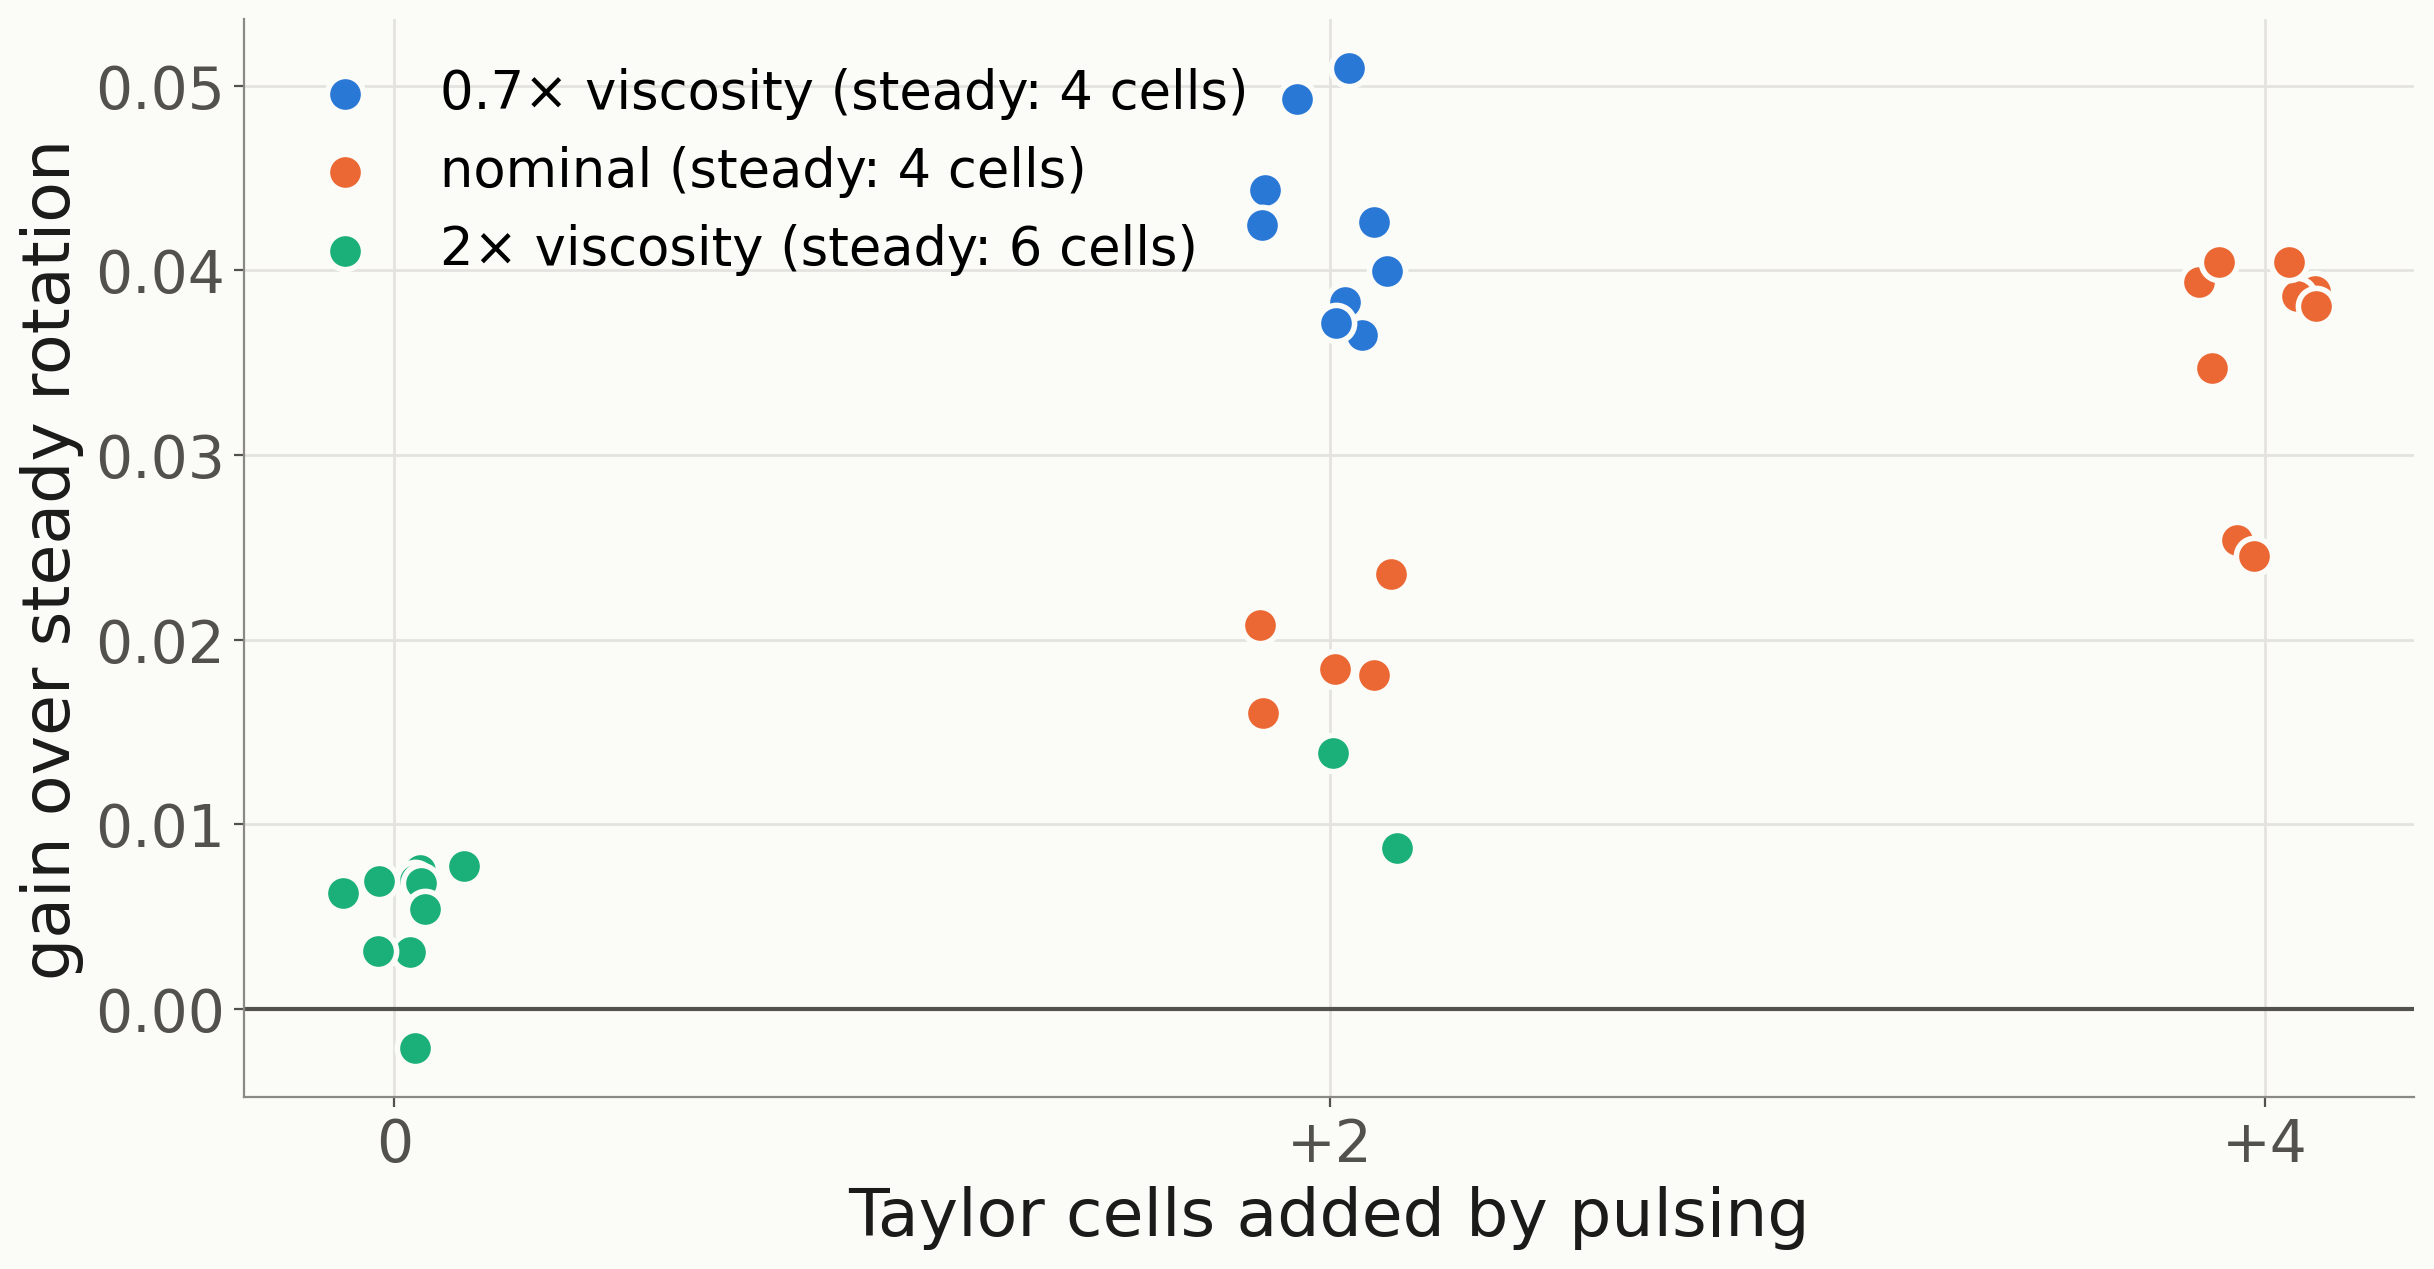
\includegraphics[width=\linewidth,height=0.72\textheight,keepaspectratio]{s_cells_added_gain}
    \end{column}
    \begin{column}{0.34\textwidth}
      At $2\times$ viscosity, steady rotation already holds 6 cells. Most pulses add none, and the gain shrinks to about +0.01.
    \end{column}
  \end{columns}
\end{frame}
\note{[Backup] Every pulsed run from the viscosity sweep, by how many cells pulsing adds over steady rotation at that viscosity. Runs that add no cells gain almost nothing; runs that add two or four gain up to five hundredths. At twice the viscosity steady rotation already has six cells, so most pulses add none. The size of the gain also depends on viscosity, so it isn't one universal curve.}

\begin{frame}{Backup: electrical power model}
  \begin{columns}[T]
    \begin{column}{0.58\textwidth}
      \begin{block}{L\'opez-Guajardo et al.\ (2024), \S3.4, Eqs.\ 18--23}
        {\small
        \[ T_{\mathrm{mot}} = \underbrace{J_{\mathrm{tot}}\,\dot\omega}_{\text{inertia}}
           + \underbrace{T_0\,\mathrm{sign}(\omega)}_{\text{bearings}}
           + \underbrace{\beta_2\,\omega^2\,\mathrm{sign}(\omega) + \beta_1\,\omega}_{\text{drag}} \]
        \[ i_{\mathrm{mot}} = \frac{T_{\mathrm{mot}}}{K_t}, \qquad
           e_{\mathrm{mot}} = L\,\frac{di_{\mathrm{mot}}}{dt} + R\,i_{\mathrm{mot}} + K_e\,\omega \]
        \[ P_{\mathrm{mot}} = e_{\mathrm{mot}}\, i_{\mathrm{mot}}, \qquad
           P_e = \begin{cases} P_{\mathrm{mot}}/\eta, & P_{\mathrm{mot}} \ge 0 \\ P_{\mathrm{mot}}\,\eta, & P_{\mathrm{mot}} < 0 \end{cases} \]}
      \end{block}
      {\small\color{ink}Evaluated on the commanded $\omega(t)$; reward uses $\overline{P_e}/P_{\max}$, $P_{\max} = 31.94$\,W (2500 rpm).}
    \end{column}
    \begin{column}{0.40\textwidth}
      {\small
      \begin{tabular*}{\linewidth}{@{}l@{\extracolsep{\fill}}r@{}}
        \toprule
        $J_{\mathrm{tot}}$ & $1.66\times10^{-4}$ kg\,m$^2$ \\
        $T_0$ & 0.1 N\,m \\
        $\beta_2$ & $7.19\times10^{-8}$ N\,m\,s$^2$ \\
        $\beta_1$ & $1.51\times10^{-5}$ N\,m\,s \\
        $K_t = K_e$ & 93.1 mN\,m/A \\
        $L$, \ $R$ & 0.28 mH, \ 0.178\,$\Omega$ \\
        $\eta$ & 0.90 \\ \bottomrule
      \end{tabular*}}\par\medskip
      {\small\color{ink}At 300 rpm the bearing term alone is $\approx$ 3.5 of the 3.7\,W, so power is set by the mean speed.}
    \end{column}
  \end{columns}
\end{frame}
\note{[Backup] The power model is the one L\'opez-Guajardo and colleagues used, Section 3.4 of their paper: motor torque from inertia, bearing friction and a quadratic drag fit; current from the torque constant; voltage from the armature circuit; electrical power with a 90 percent controller efficiency, and regeneration when braking. We evaluate it on the commanded speed and normalize by the power at 2500 rpm, 31.94 watts. At 300 rpm almost all of the 3.7 watts is bearing friction, which depends only on speed, so fixing the mean speed fixes the power, whatever the waveform's shape.}

\end{document}
"   (x2)
%                                                    -> talk_notes.pdf (slides + speaker notes)
% Figures: ../figures (make_slide_figures.py) and ../../poster_2026-10-02.
\documentclass[aspectratio=169,11pt]{beamer}
\usetheme{default}
\usepackage{lmodern}
\setbeamertemplate{navigation symbols}{}
\setbeamertemplate{blocks}[rounded][shadow=false]
\setbeamertemplate{footline}[frame number]
\setbeamertemplate{itemize items}[circle]
\usepackage[utf8]{inputenc}
\usepackage[T1]{fontenc}
\usepackage{amsmath,amssymb,bm}
\usepackage{booktabs}
\usepackage{tikz}
\usetikzlibrary{arrows.meta}
\graphicspath{{../figures/}{../../poster_2026-10-02/}{../../}}

\ifdefined\withnotes
  \setbeameroption{show notes}
  \setbeamertemplate{note page}[plain]
\fi

% ---- University of Houston palette (from the UH URD template) ---------------
% UH Red #C8102E, Brick #960C22, Slate #54585A; logos cut from the template's banner.
\definecolor{uhred}{HTML}{C8102E}
\definecolor{uhbrick}{HTML}{960C22}
\definecolor{uhslate}{HTML}{54585A}
\definecolor{navy}{HTML}{231F20}     % primary text (near-black)
\definecolor{ink}{HTML}{54585A}      % secondary text (UH slate)
\definecolor{accent}{HTML}{C8102E}
\definecolor{accentdk}{HTML}{960C22}
\definecolor{paper}{HTML}{FBFBF8}    % matches the figure backgrounds
\definecolor{card}{HTML}{F1F0EE}
\definecolor{vblue}{HTML}{1C5CAB}
\setbeamercolor{normal text}{fg=navy,bg=paper}
\setbeamercolor{frametitle}{fg=white,bg=uhred}
\setbeamercolor{alerted text}{fg=uhred}
\setbeamercolor{block title}{fg=uhbrick,bg=card}
\setbeamercolor{block body}{fg=ink,bg=card}
\setbeamercolor{structure}{fg=uhred}
\setbeamercolor{page number in head/foot}{fg=uhslate}
\setbeamerfont{block title}{size=\small,series=\bfseries}
\setbeamertemplate{frametitle}{%
  \nointerlineskip%
  \begin{beamercolorbox}[wd=\paperwidth,ht=7.5mm,dp=2.8mm,leftskip=4.5mm,rightskip=3.5mm]{frametitle}%
    \usebeamerfont{frametitle}\insertframetitle\hfill\raisebox{-1.7mm}{
\includegraphics[height=6.2mm]{uh/uh_mark_white}}%
  \end{beamercolorbox}%
  \vspace{1mm}}

\newcommand{\takeaway}[1]{\par\smallskip{\color{ink}#1}\par}
\newcommand{\bignum}[2]{{\usebeamerfont{title}\color{navy}\LARGE\bfseries #1}\\[-1pt]{\small\color{ink}#2}}

\title{Brief stops, more vortices}
\subtitle{Deep reinforcement learning discovers transferable control strategies for catalytic-wall Taylor--Couette reactors}
\author{Isaiah N.\ Bascom\inst{1} \and Min Wang\inst{1} \and Yuhe Wang\inst{2}}
\institute{\inst{1}Department of Mathematics, University of Houston, Houston, Texas \and \inst{2}Institute for Scientific Computation, Texas A\&M University, College Station, Texas}
\date{GCURS 2026 \textbullet\ Computational \& Applied Mathematics}

\begin{document}

% ============================================================================
\begin{frame}[plain]
  \begin{tikzpicture}[remember picture,overlay]
    \fill[uhred] (current page.north west) rectangle ([yshift=-15mm]current page.north east);
    \node[anchor=west] at ([xshift=6mm,yshift=-7.5mm]current page.north west) {
\includegraphics[height=9.5mm]{uh/uh_mark_white}};
    \node[anchor=east] at ([xshift=-6mm,yshift=-7.5mm]current page.north east) {
\includegraphics[height=10.5mm]{uh/uh_wordmark_white}};
    \node[anchor=center, text=white, font=\scriptsize\bfseries] at ([yshift=-7.5mm]current page.north) {GCURS 2026 \textbullet\ COMPUTATIONAL \& APPLIED MATHEMATICS};
    \node[anchor=north west, text width=148mm, align=left, inner sep=0pt, text=navy, font=\usebeamerfont{title}\huge\bfseries]
      at ([xshift=6mm,yshift=-20mm]current page.north west) {Brief stops, more vortices};
    \node[anchor=north west, inner sep=0pt, text=ink]
      at ([xshift=6mm,yshift=-31mm]current page.north west) {\resizebox{148mm}{!}{Deep reinforcement learning discovers transferable control strategies for catalytic-wall Taylor--Couette reactors}};
    \node[anchor=north, inner sep=0pt] at ([yshift=-40mm]current page.north)
      {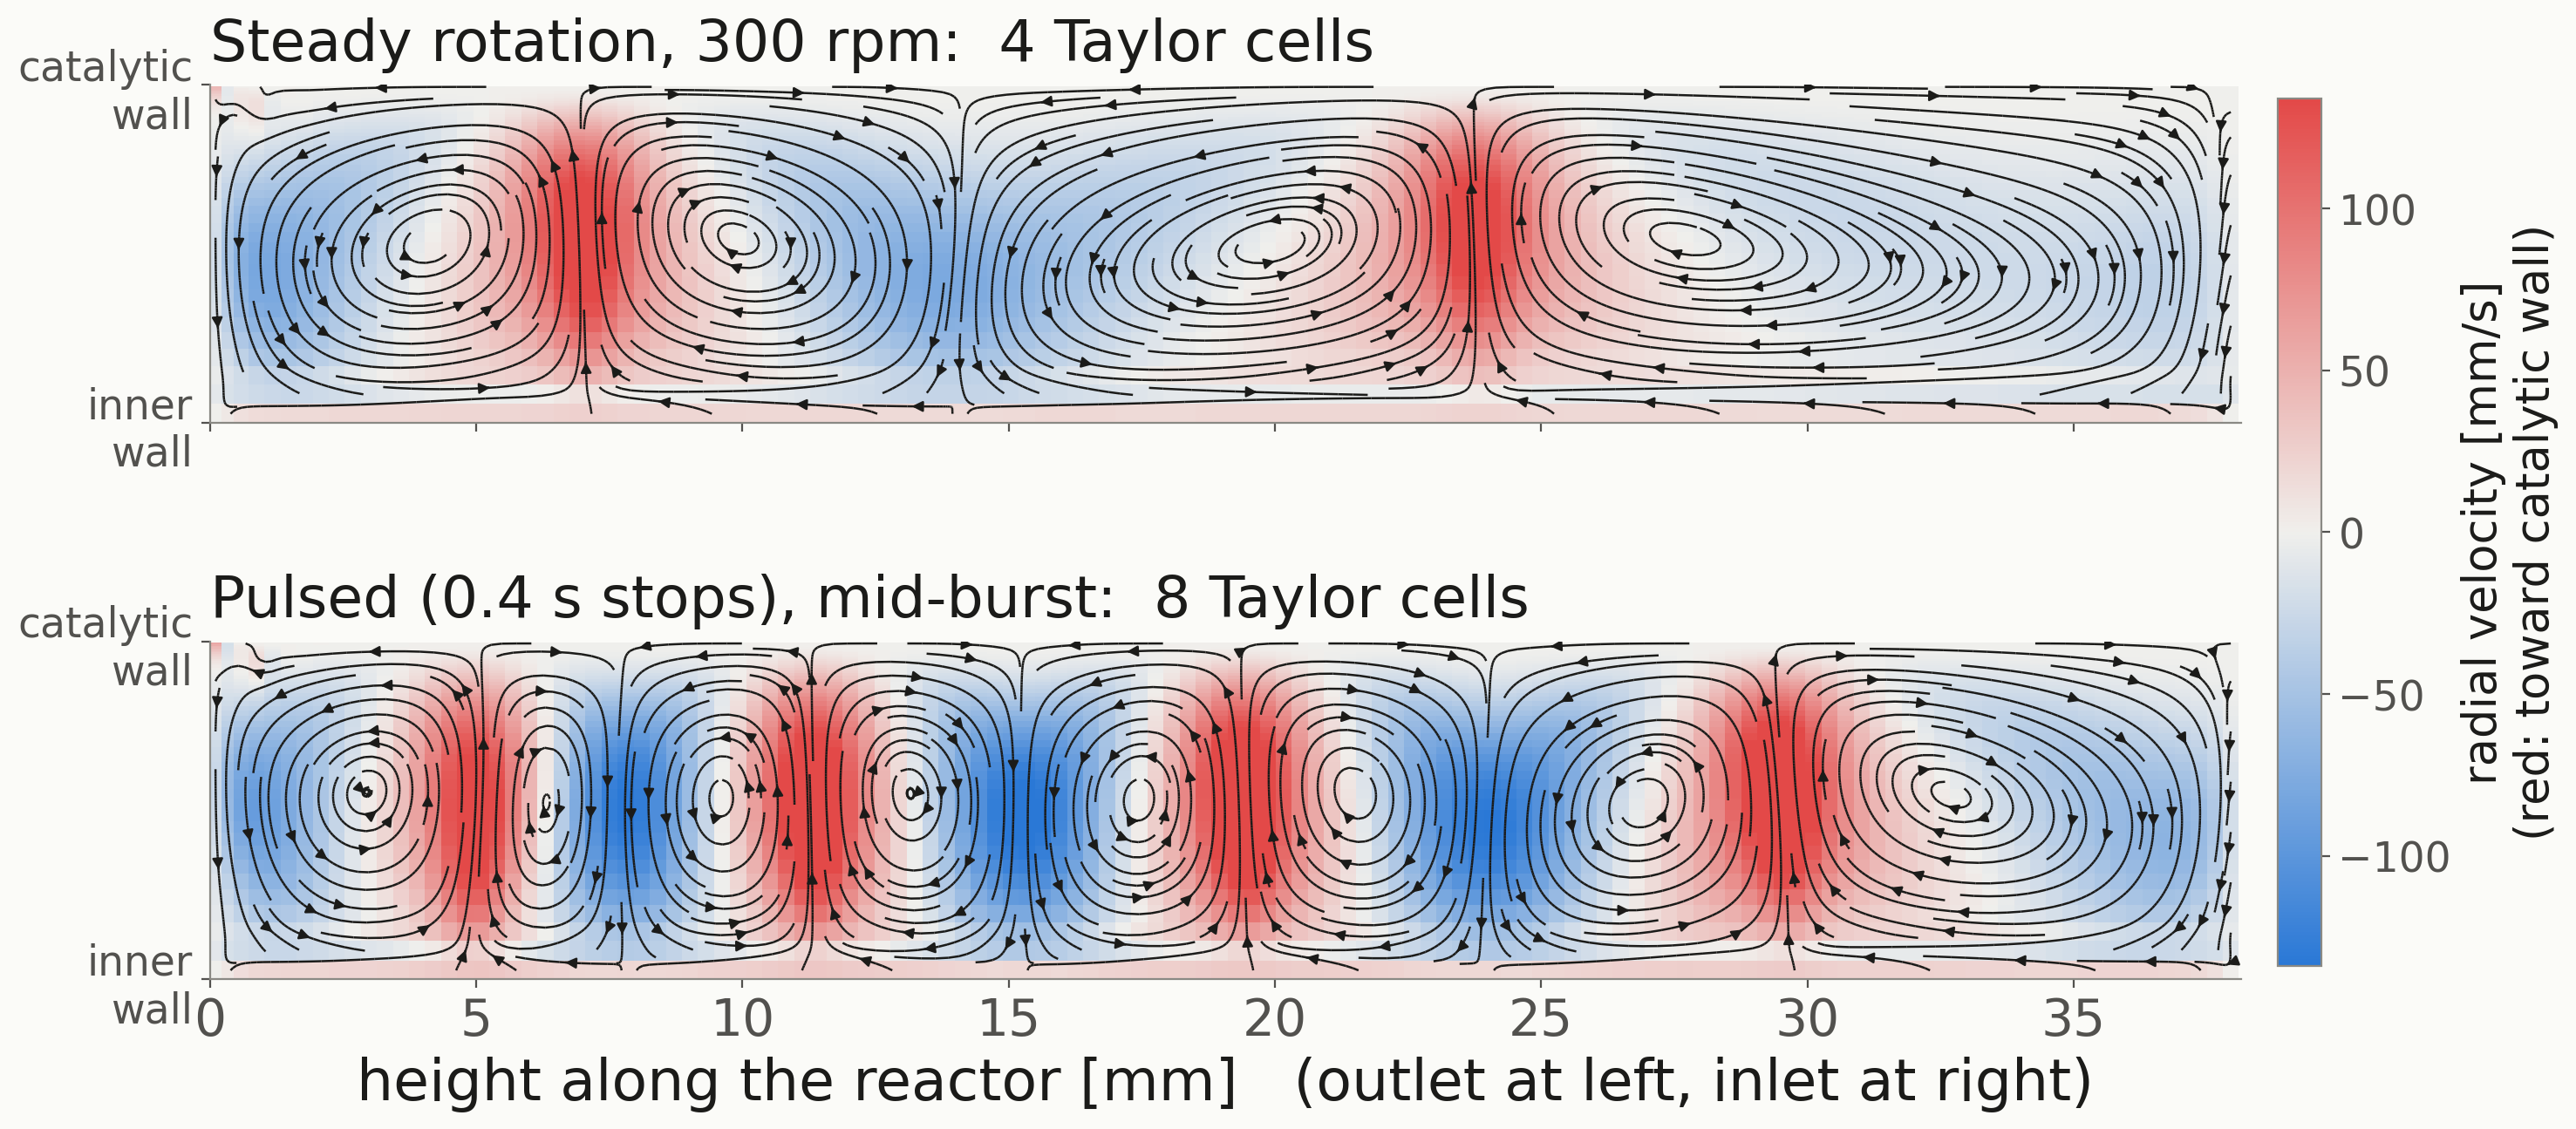
\includegraphics[width=148mm,height=30mm,keepaspectratio]{s_cells_snapshot}};
    \node[anchor=south west, inner sep=0pt, text=navy, font=\bfseries] at ([xshift=6mm,yshift=11.5mm]current page.south west)
      {Isaiah N.\ Bascom$^{1}$, \ Min Wang$^{1}$, \ Yuhe Wang$^{2}$};
    \node[anchor=south west, inner sep=0pt, text=ink, font=\scriptsize, align=left] at ([xshift=6mm,yshift=4mm]current page.south west)
      {$^{1}$Department of Mathematics, University of Houston, Houston, Texas\\
       $^{2}$Institute for Scientific Computation, Texas A\&M University, College Station, Texas};
  \end{tikzpicture}
\end{frame}
\note{[0:30] Hi, I'm Isaiah Bascom. I work on Taylor--Couette reactors: a liquid fills the gap between two cylinders, the inner one spins, and a catalyst coats the outer wall. Today's story has two parts. First, a reinforcement-learning agent found a surprisingly simple way to run this reactor better: brief full stops. Second, we found out why it works. The picture is the punchline: steady rotation gives four vortex cells, and pulsed rotation gives eight.}

% ============================================================================
\begin{frame}{The Taylor--Couette reactor}
  \begin{columns}[c]
    \begin{column}{0.60\textwidth}
      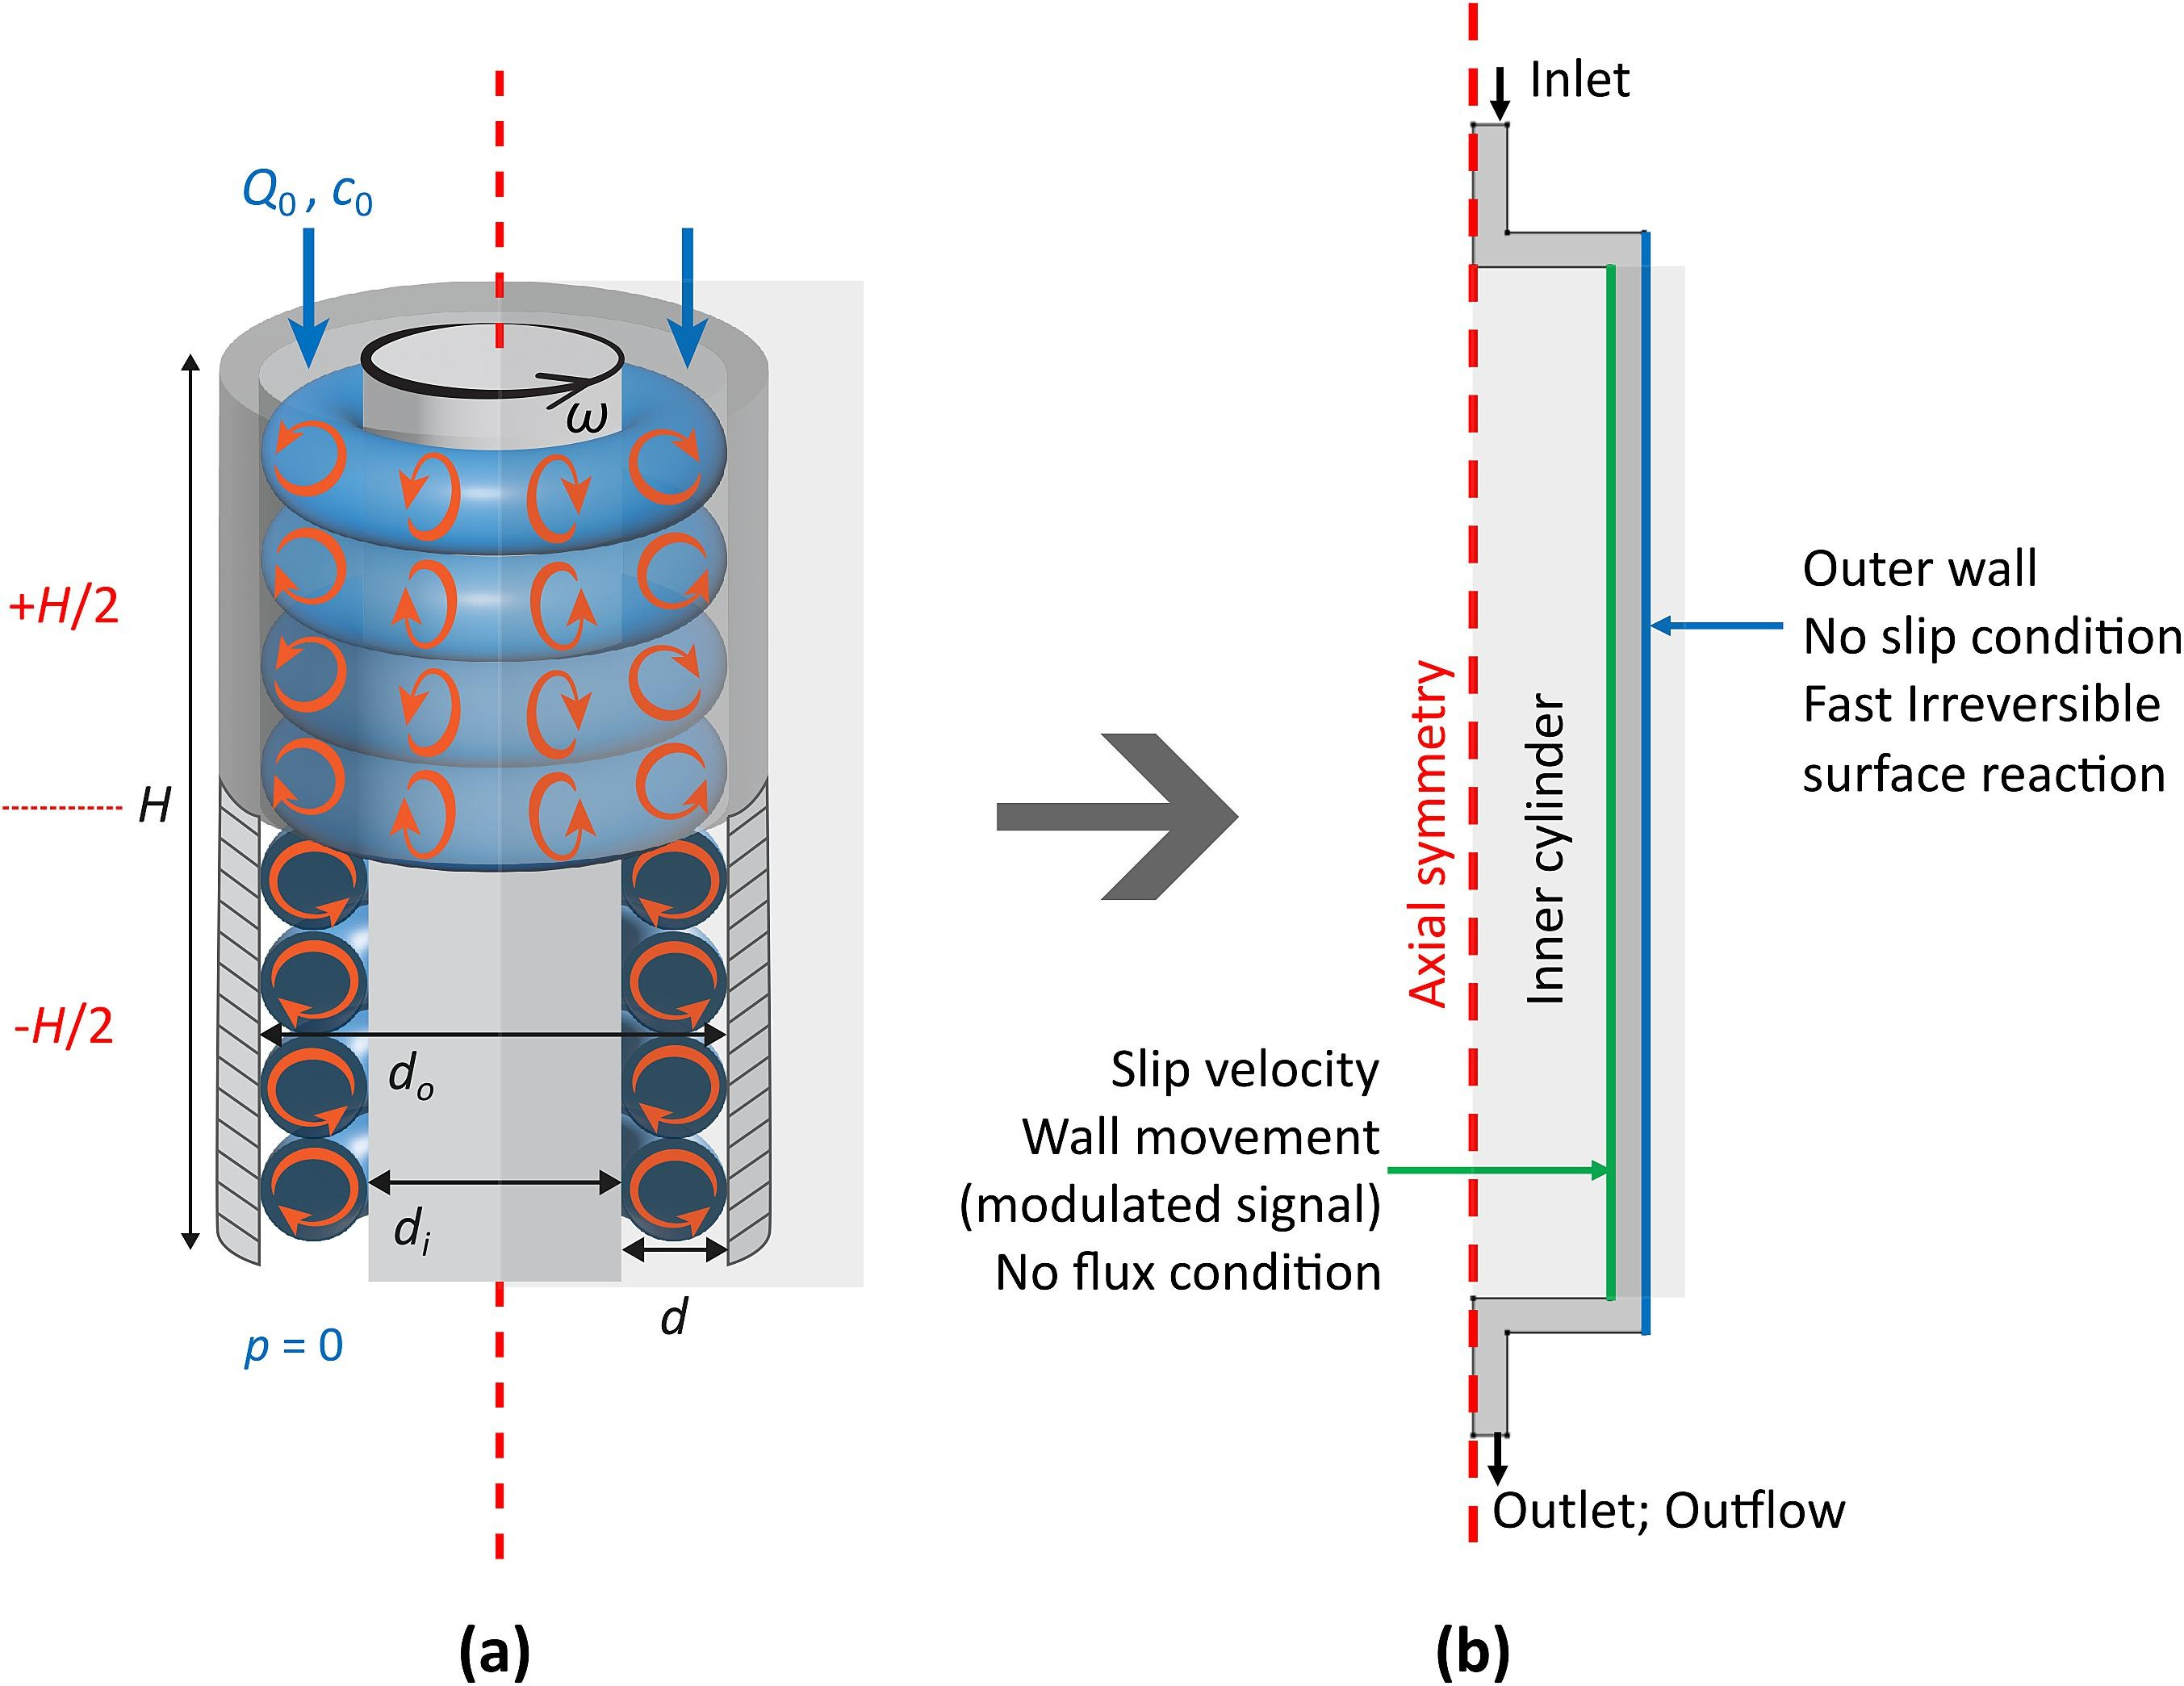
\includegraphics[width=\linewidth,height=0.78\textheight,keepaspectratio]{lg-reactor}\par
      {\tiny\color{ink}Figure: L\'opez-Guajardo et al., \emph{Chem.\ Eng.\ J.} 489 (2024) 151174, Fig.~2.}
    \end{column}
    \begin{column}{0.36\textwidth}
      {\small
      \begin{tabular*}{\linewidth}{@{}l@{\extracolsep{\fill}}r@{}}
        \toprule
        Gap $d$ & 6.35 mm \\
        $d_i$ / $d_o$ & 50.8 / 63.5 mm \\
        Height $H$ & 190.5 mm \\
        $\Gamma = H/d$ & 30 \\
        Feed $Q_0$ & 100 mL/min \\ \bottomrule
      \end{tabular*}}\par\bigskip
      Inner cylinder spins; catalyst on the outer wall.
    \end{column}
  \end{columns}
\end{frame}
\note{[0:45] First, the general setup. A Taylor--Couette reactor is liquid in the gap between two cylinders. The inner one spins, which sets up the stacked ring vortices you see on the left, the Taylor vortices. Feed enters at the top and leaves at the bottom, and the outer wall is coated with catalyst, so the reaction happens only there. The gap is about six millimetres, the reactor is about nineteen centimetres tall, an aspect ratio of thirty. Because the flow is symmetric around the axis, we can simulate just a two-dimensional slice, shown on the right; that's the standard reduction, and it's what makes reinforcement learning on this problem affordable.}

% ============================================================================
\begin{frame}{The reaction happens only at the wall}
  \begin{columns}[c]
    \begin{column}{0.52\textwidth}
      Taylor vortices carry reactant to the catalytic wall.\par\bigskip
      \begin{block}{Problem}
        Choose $\omega(t)$ for the most conversion per unit power.
      \end{block}
    \end{column}
    \begin{column}{0.46\textwidth}
      \centering
      % 2D axisymmetric domain (cf. Lopez-Guajardo et al. Fig. 2b): the fluid gap is the
      % real CFD field under the learned RL policy; everything else is drawn.
      \begin{tikzpicture}[x=1mm, y=1mm, every node/.style={font=\scriptsize}]
        \def\H{46}            % drawn height of the gap [mm]; width = H/6 (true 6.35:38.1)
        \def\W{7.67}
        \def\xg{14}           % left edge of the fluid gap
        % axis of symmetry
        \draw[uhred, dashed, line width=0.8pt] (0,-3) -- (0,\H+4);
        \node[rotate=90, text=uhred, font=\tiny] at (-2.2,\H/2) {axis of symmetry};
        % inner cylinder (schematic, not to scale in r)
        \fill[black!25] (3,0) rectangle (\xg,\H);
        \node[rotate=90, align=center, font=\tiny] at (8.5,\H/2) {inner cylinder, $\omega(t)$};
        % fluid gap: real field
        \node[anchor=south west, inner sep=0] at (\xg,0) {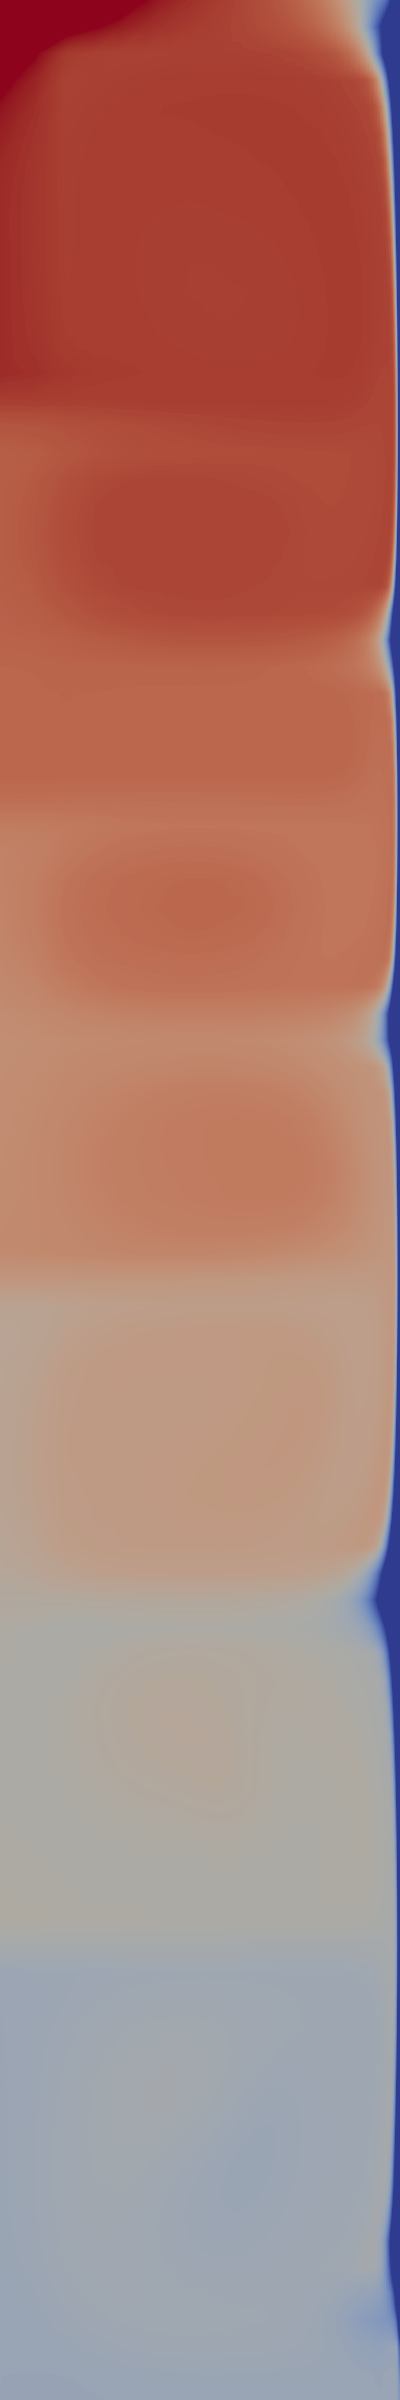
\includegraphics[width=\W mm,height=\H mm]{rl_flow_2d_conc_crop}};
        % bottom wall and catalytic outer wall (outer wall stops above the side outlet)
        \draw[black!60, line width=1.2pt] (\xg,0) -- (\xg+\W,0);
        \definecolor{wallblue}{HTML}{3B4CC0}   % bottom of the concentration scale: c = 0
        \draw[wallblue, line width=1.6pt] (\xg+\W+0.6,1.4) -- (\xg+\W+0.6,\H);
        % inlet at the top of the gap
        \draw[-{Latex[length=2mm]}, navy, line width=1pt] (\xg+\W/2,\H+6) -- (\xg+\W/2,\H+0.6);
        \node[anchor=south] at (\xg+\W/2,\H+6) {inlet};
        % side outlet: the bottom 0.42 mm of the outer wall
        \draw[-{Latex[length=2mm]}, navy, line width=1pt] (\xg+\W+0.2,0.7) -- (\xg+\W+7,0.7);
        \node[anchor=west, align=left] at (\xg+\W+7.3,0.9) {\textbf{side outlet}};
        % labels
        \node[anchor=west, align=left, text=wallblue, font=\scriptsize\bfseries] at (\xg+\W+2.2,\H*0.62)
          {catalytic wall\\[-1pt]{\normalfont\tiny $c = 0$}};
        % concentration key (ParaView "Cool to Warm", matching the render's 0.45-0.88 c/c0 range)
        \definecolor{cw0}{HTML}{3B4CC0}\definecolor{cw1}{HTML}{DDDDDD}\definecolor{cw2}{HTML}{B40426}
        \shade[bottom color=cw0, top color=cw1] (\xg+\W+3,\H*0.22) rectangle (\xg+\W+5,\H*0.32);
        \shade[bottom color=cw1, top color=cw2] (\xg+\W+3,\H*0.32) rectangle (\xg+\W+5,\H*0.42);
        \node[anchor=west, font=\tiny, text=ink] at (\xg+\W+5.4,\H*0.42) {reactant};
        \node[anchor=west, font=\tiny, text=ink] at (\xg+\W+5.4,\H*0.22) {product};
      \end{tikzpicture}\par\smallskip
    \end{column}
  \end{columns}
\end{frame}
\note{[0:45] The reaction only happens on the catalytic outer wall, so everything depends on how fast reactant gets carried from the bulk to that wall. The Taylor vortices in the gap do that carrying. Changing the rotation over time can beat spinning at a constant speed. The picture is the 2D plane our simulation actually solves on, with the real flow under the learned policy: the spinning inner cylinder on the left, the liquid gap coloured by concentration, and the catalytic wall on the right. Red is fresh reactant; blue is where it has been converted to product. You can see the thin blue layer along the catalytic wall, and the vortices peeling that converted liquid off the wall and bringing fresh reactant in. Fluid enters at the top and leaves through a side outlet at the bottom of the outer wall. So this is a control problem governed by PDEs: choose the speed as a function of time to get the most reactant converted for the power spent. What is the optimal control, and why does it work?}

% ============================================================================
\begin{frame}{Non-turbulent flow and scalar transport}
  \begin{columns}[T]
    \begin{column}{0.56\textwidth}
      \begin{block}{Equations}
        \setlength{\abovedisplayskip}{5pt}\setlength{\belowdisplayskip}{5pt}%
        Laminar incompressible flow with constant viscosity and no turbulence model
        \begin{gather*}
          \nabla\cdot\mathbf{u} = 0\\
          \frac{\partial\mathbf{u}}{\partial t} + (\mathbf{u}\cdot\nabla)\mathbf{u} = -\nabla p + \nu\,\nabla^2\mathbf{u}
        \end{gather*}
        Scalar-transport equation
        \[ \frac{\partial c}{\partial t} + \mathbf{u}\cdot\nabla c = D\,\nabla^2 c \]
      \end{block}
    \end{column}
    \begin{column}{0.40\textwidth}
      \begin{block}{Numerics}
        Finite volume (OpenFOAM), 2D axisymmetric; 3330 cells graded to 25\,$\mu$m at the catalytic wall\par\smallskip
        Inner wall: $\omega(t)$\\ Catalytic wall: $c = 0$\\ Inlet: $c = c_0$\par\smallskip
        $\mathrm{Re}\approx 470$, \ $\mathrm{Sc}=1075$
      \end{block}
    \end{column}
  \end{columns}
  \medskip
  \begin{beamercolorbox}[wd=\textwidth,sep=8pt,rounded=true]{frametitle}
    \begin{tabular}{@{}l@{\ }l@{}}
      \textbf{Objective:} & $\max\; X - P/P_{\max}$ \quad s.t. \ $\overline{\omega} = 300$ rpm\\[2pt]
      & {\small $X = 1 - \bar c_{\mathrm{out}}/c_0$ (conversion), \ $P$ = motor power}
    \end{tabular}
  \end{beamercolorbox}
\end{frame}
\note{[0:45] Incompressible Navier--Stokes for the flow, solved axisymmetrically but keeping the swirl component, and an advection--diffusion equation for the reactant. The inner wall turns at a prescribed omega of t. On the catalytic wall the concentration is zero, so the reaction rate is set entirely by how fast reactant diffuses in. Finite-volume discretization in OpenFOAM, with the mesh graded to 25 microns at the wall because the concentration layer there is thin: the Schmidt number is about a thousand. The objective rewards conversion and penalizes motor power. We also fix the mean speed at 300 rpm, which in practice fixes the power, so every candidate is compared at the same power and the question becomes how much conversion each one gets for it.}

% ============================================================================
\begin{frame}{Three ways to search an expensive simulator}
  \begin{columns}[T]
    \begin{column}{0.32\textwidth}
      \begin{block}{\begin{tabular}[t]{@{}l@{\ }l@{}}Discover: & reinforcement\\ & learning\end{tabular}}
        TD3 actor--critic. State: conversion and time. Action: burst and stop lengths. Reward: conversion. No physics given.
      \end{block}
    \end{column}
    \begin{column}{0.32\textwidth}
      \begin{block}{\begin{tabular}[t]{@{}l@{\ }l@{}}Check: & Bayesian\\ & optimization\end{tabular}}
        Gaussian-process surrogate (Mat\'ern-5/2) with expected improvement; 220 CFD runs over fixed waveforms. Replicate noise $\sigma\approx 0.002$.
      \end{block}
    \end{column}
    \begin{column}{0.32\textwidth}
      \begin{block}{\begin{tabular}[t]{@{}l@{\ }l@{}}Explain: & designed\\ & experiments\end{tabular}}
        Pre-registered hypotheses, 62 targeted runs, flow diagnostics logged every 0.02\,s.
      \end{block}
    \end{column}
  \end{columns}
  \bigskip
  \takeaway{Each 130\,s simulation costs about 3--4 CPU-hours, so every method has to be sample-efficient.}
\end{frame}
\note{[0:45] Each simulated episode costs a few CPU-hours, so I used three complementary tools. Reinforcement learning, with TD3, an actor--critic method, to discover a strategy without being told any physics: it sees only the conversion and the time, and chooses how long to run and how long to stop. Bayesian optimization, with a Gaussian-process surrogate and expected improvement over 220 simulations, as an independent check. And designed experiments, with hypotheses written down in advance, to explain why the answer works.}

% ============================================================================
\begin{frame}{Reinforcement learning found brief full stops}
  \alert{All 5 runs: brief full stops (0.1--0.4\,s), never long idles.}\par\medskip
  \centering\includegraphics[width=\linewidth,height=0.66\textheight,keepaspectratio]{fig4_learned_waveform}
\end{frame}
\note{[0:45] Here's what the reinforcement-learning agent did, with the average held at 300 rpm. What it learned, in all five independent training runs, is the same kind of policy: run a little above 300 rpm for a few seconds, then stop completely for a fraction of a second, mostly a tenth to four tenths of a second, and repeat. None of them learned long idles. That was not the answer I expected, and it's the opposite of the published recipe.}

% ============================================================================
\begin{frame}{The opposite of the published recipe}
  \begin{columns}[c]
    \begin{column}{0.60\textwidth}
      \includegraphics[width=\linewidth,height=0.74\textheight,keepaspectratio]{fig5_recipe_contrast}
    \end{column}
    \begin{column}{0.38\textwidth}
      \begin{block}{Bayesian optimization}Stop 0.5\,s every 5\,s\end{block}
      \begin{block}{RL}Within 0.01--0.02 of it\end{block}
      \begin{block}{Published recipe}Best in their model, not ours\end{block}
    \end{column}
  \end{columns}
\end{frame}
\note{[0:45] On top, the published recipe: burst to 2500 rpm for six seconds, then sit still for twenty-four. Below, what the agent found. The Bayesian-optimization search over 220 fixed waveforms found the same thing: stop for about half a second every five seconds. The learned policies stop a little shorter, mostly 0.1 to 0.4 seconds, and come within one to two hundredths of conversion of that best fixed waveform, so RL matched the search rather than beating it. Later we'll see why the shorter stops cost a little: they mostly land in the six-cell state rather than eight. The published recipe was the best policy in their model, but in ours it loses even to steady rotation. One note: my submitted abstract describes long low-speed periods with short bursts. The result turned out to be the opposite, brief full stops at high duty, and this slide is the correction.}

% ============================================================================
\begin{frame}{It transfers to a reactor five times taller}
  \begin{columns}[c]
    \begin{column}{0.52\textwidth}
      \includegraphics[width=\linewidth,height=0.74\textheight,keepaspectratio]{fig1_conversion_vs_power}
    \end{column}
    \begin{column}{0.46\textwidth}
      {\small
      \begin{tabular*}{\linewidth}{@{}l@{\extracolsep{\fill}}r@{}}
        \toprule
        Tall reactor & Conversion \\ \midrule
        RL, no retraining & 0.90 \\
        Best fixed waveform & 0.91 \\
        Steady, same power & 0.79 \\
        Published, $1.7\times$ power & 0.76 \\ \bottomrule
      \end{tabular*}}
    \end{column}
  \end{columns}
\end{frame}
\note{[0:45] Then a generalization test: the policy trained on the short reactor, run with no retraining on a reactor five times taller. The blue line is steady rotation at different speeds. The red star is the transferred policy: 0.90 conversion at 3.7 watts, against 0.79 for steady rotation at the same power. It ties the best fixed waveform at 0.91. The grey triangle is the published recipe: 0.76 while using about 1.7 times the power. Caveat in small print: these tall-reactor runs used the original time step, so trust the ranking more than the third decimal.}

% ============================================================================
\begin{frame}{Why it works: each restart builds more vortex cells}
  \centering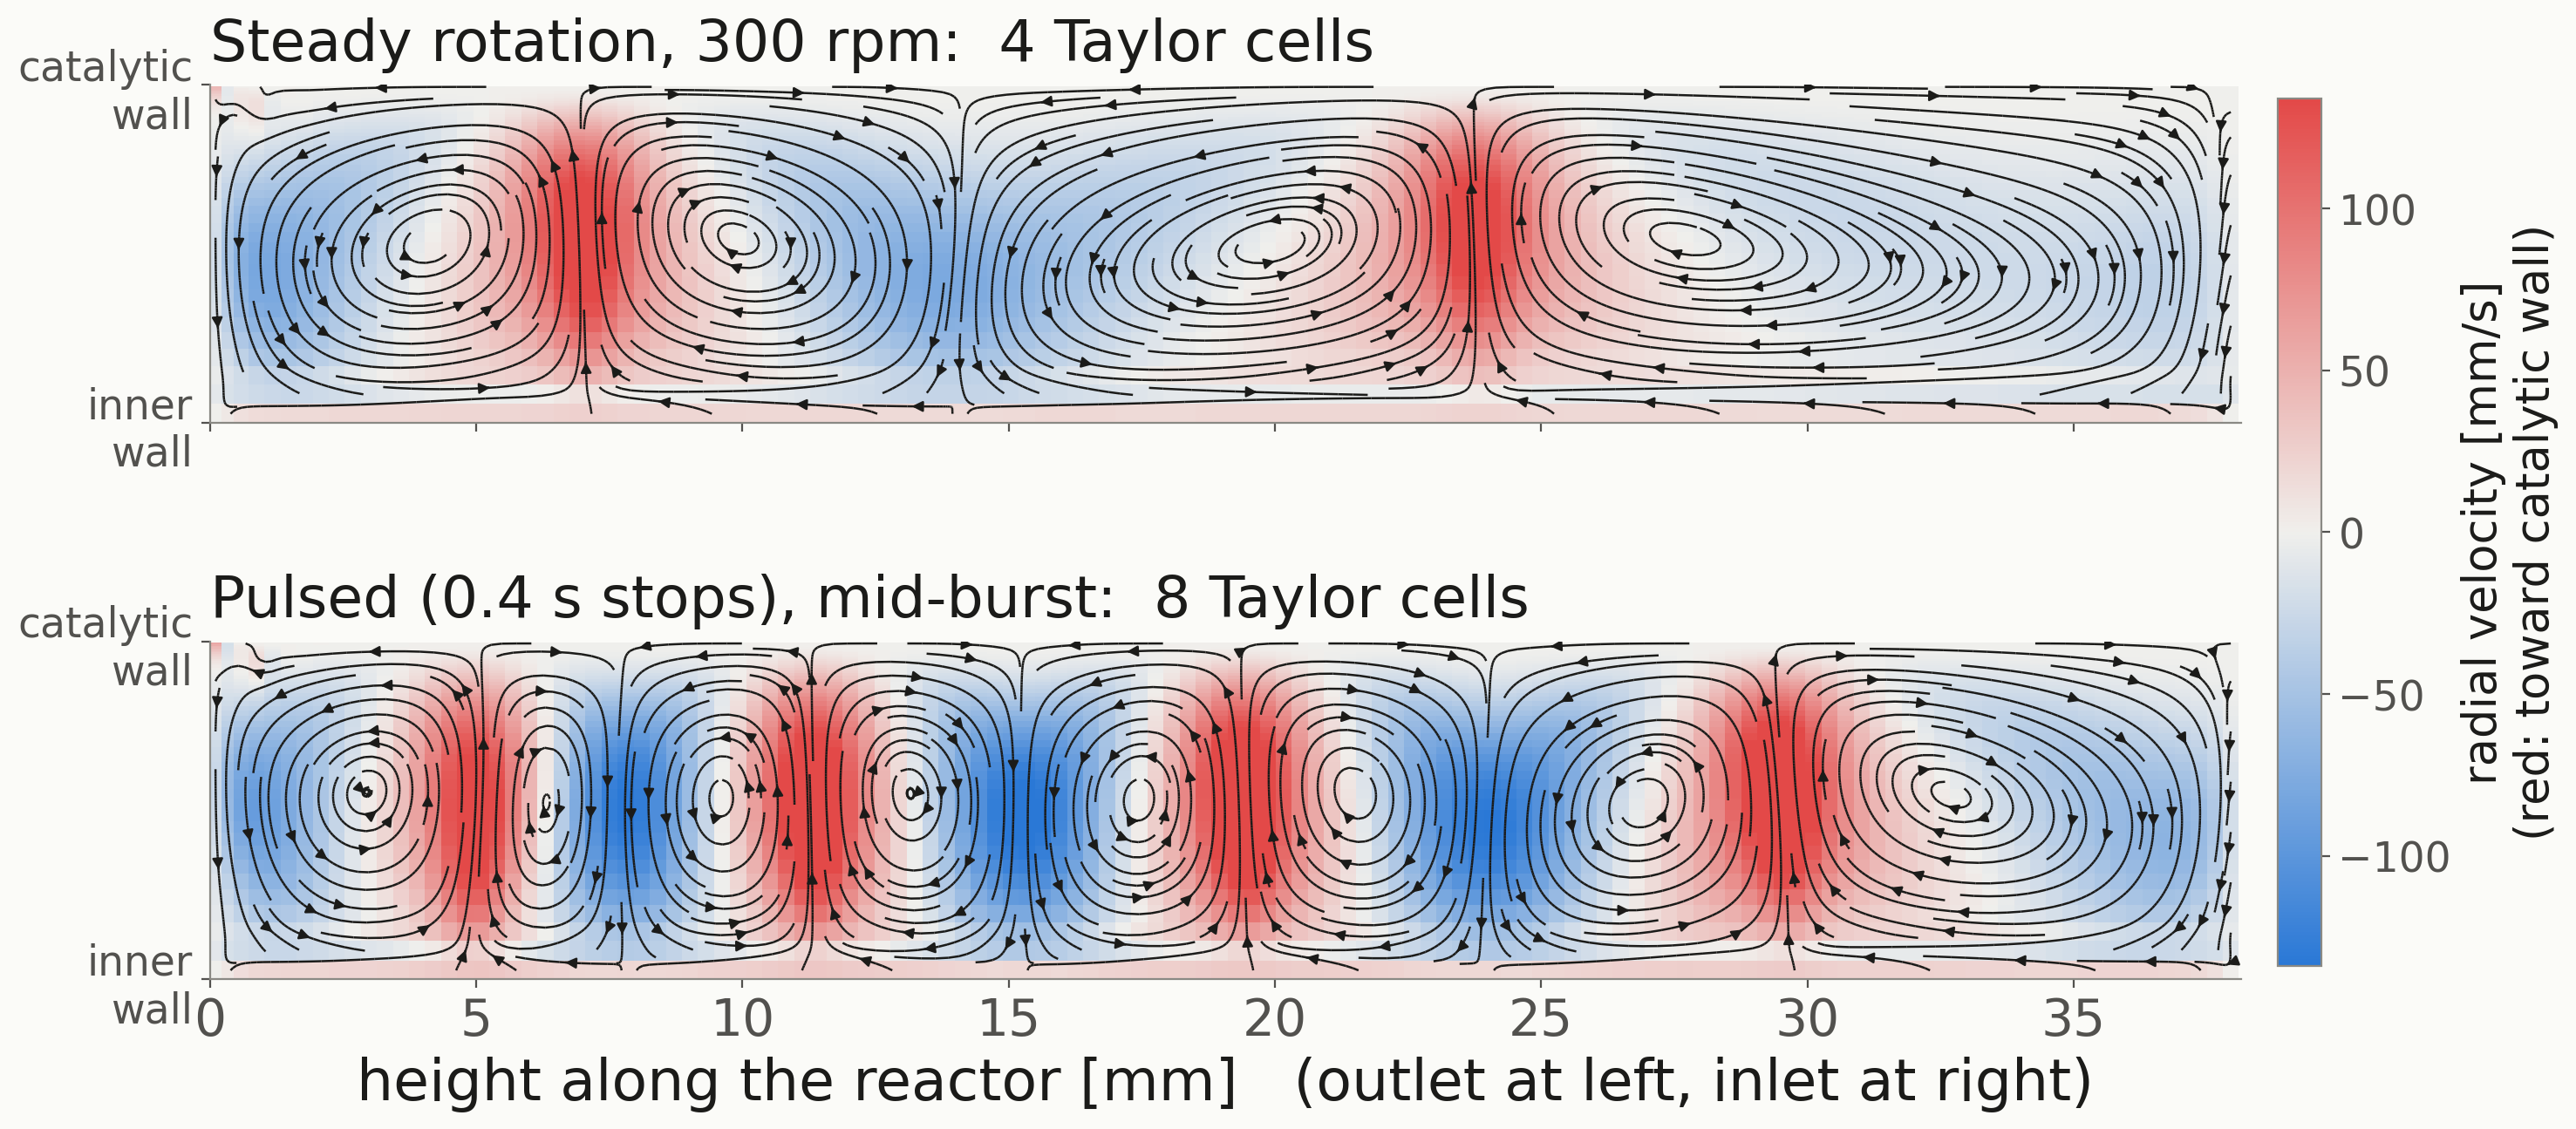
\includegraphics[width=\linewidth,height=0.86\textheight,keepaspectratio]{s_cells_snapshot}
\end{frame}
\note{[1:00] So why does a brief stop help? Both panels show the gap between the cylinders, unrolled sideways: inner wall at the bottom, catalytic wall at the top. Colour is radial velocity; red means liquid heading toward the catalytic wall. Under steady rotation there are four large vortex cells. Under pulsing, mid-burst, there are eight narrower ones. In dynamical-systems language this is multistability: at the same Reynolds number a short Taylor--Couette annulus has several stable solutions with different numbers of cells, and which one you land in depends on the initial condition; Benjamin and Mullin studied this in the early 1980s (check citation). Each brief stop brings the flow nearly to rest, and the restart from rest selects a higher axial wavenumber, eight cells instead of four. Narrower cells carry reactant to the wall faster.}

% ============================================================================
\begin{frame}{Restarts make the extra cells; steady rotation erases them}
  \begin{columns}[T]
    \begin{column}{0.49\textwidth}
      \centering{\small\textbf{Each cycle:} 8 cells, +15\% wall reaction}\par\smallskip
      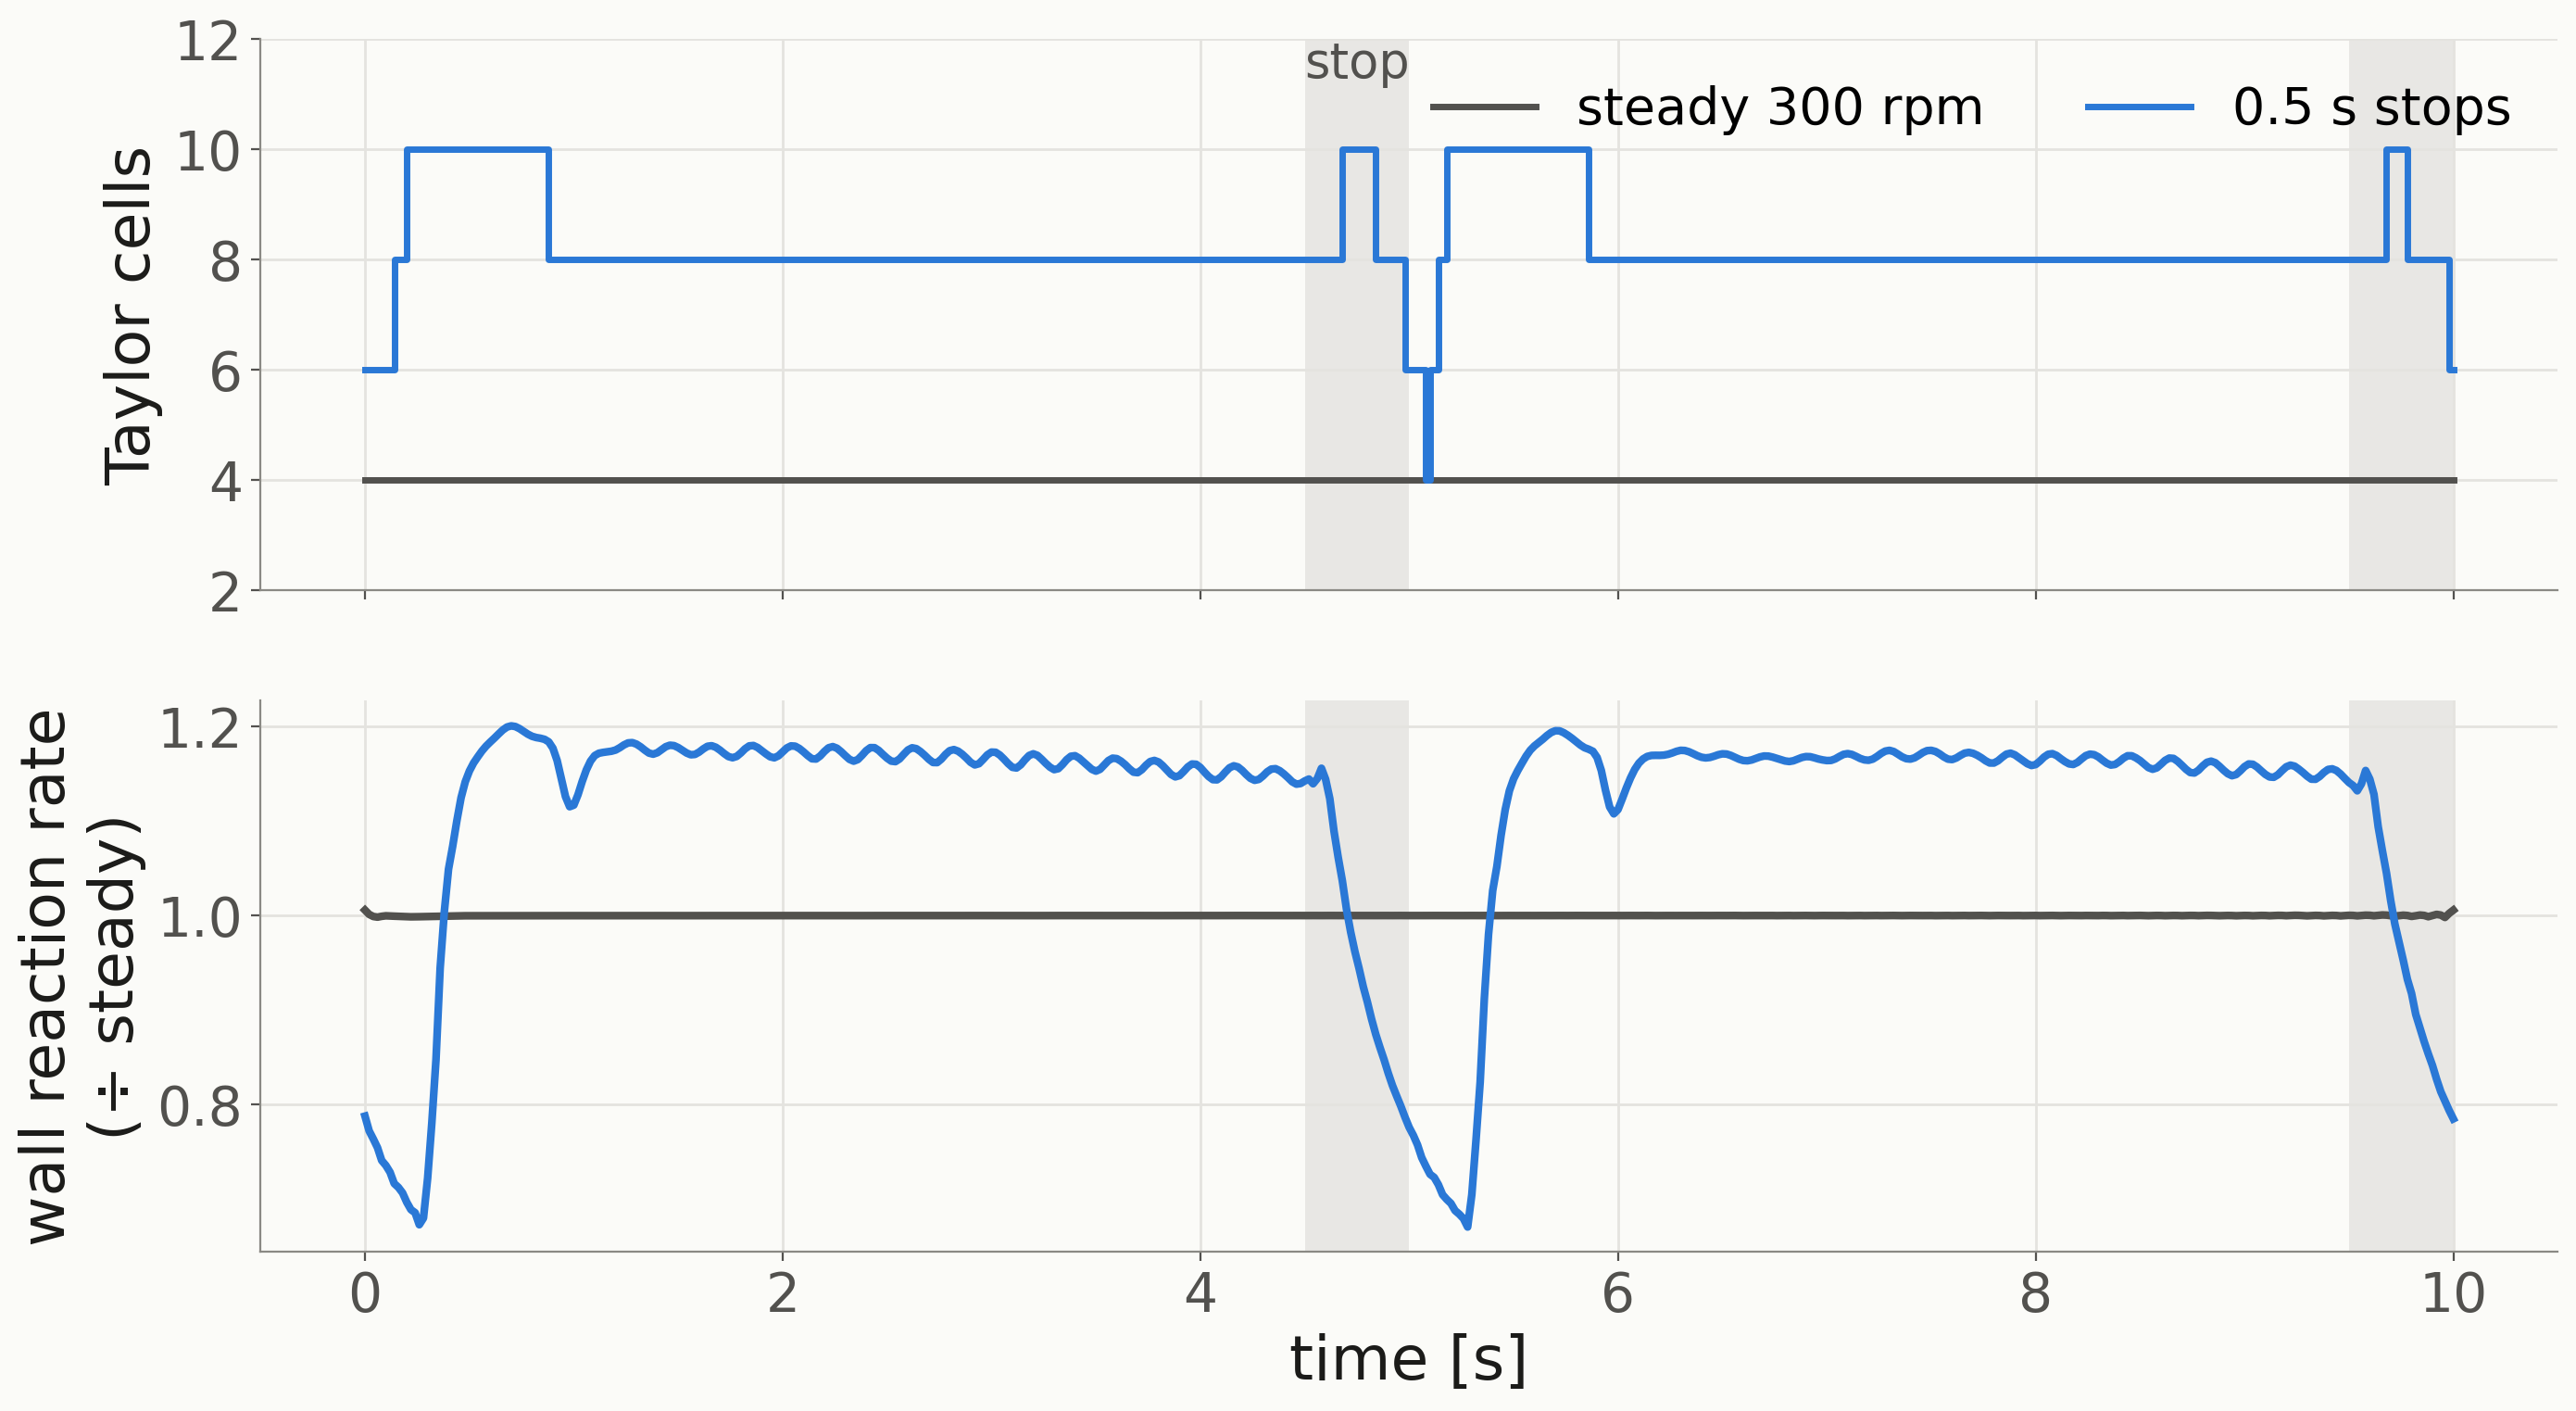
\includegraphics[width=\linewidth,height=0.56\textheight,keepaspectratio]{s_one_cycle}
    \end{column}
    \begin{column}{0.49\textwidth}
      \centering{\small\textbf{Stop pulsing:} back to 4 cells in 10--15\,s}\par\smallskip
      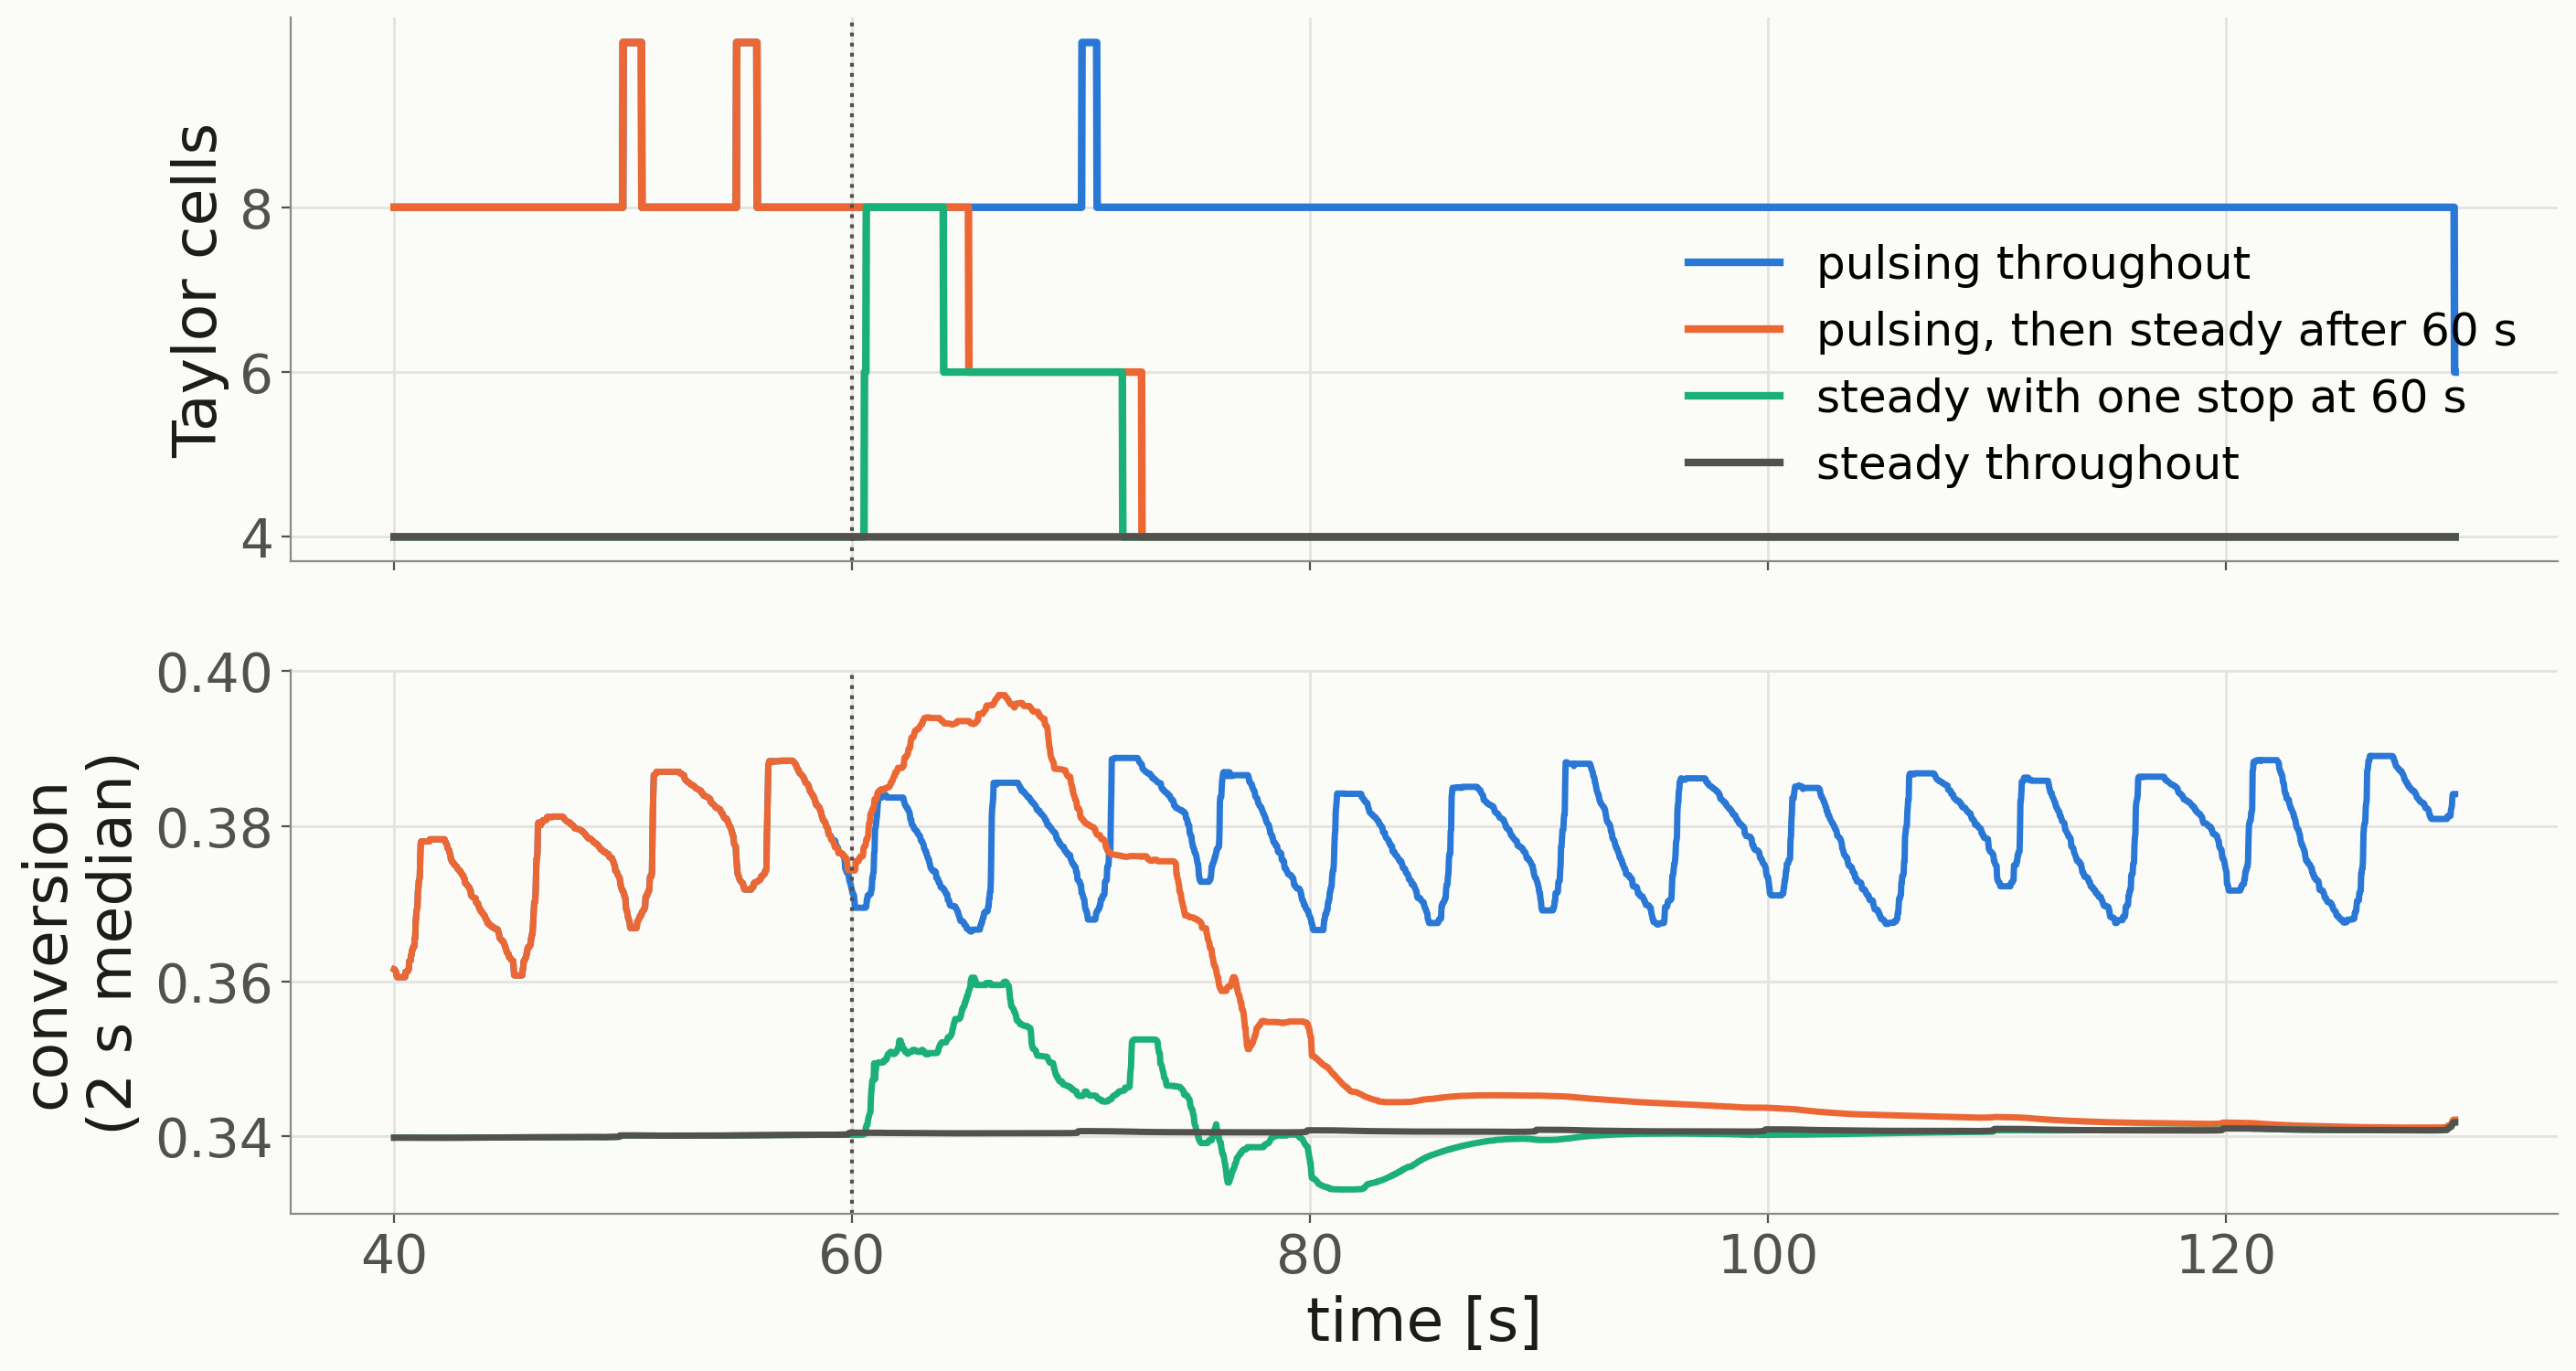
\includegraphics[width=\linewidth,height=0.56\textheight,keepaspectratio]{s_hold_kick}
    \end{column}
  \end{columns}
  \medskip
  \centering\alert{\textbf{Stops must repeat.}}
\end{frame}
\note{[1:00] Inside each cycle: after every restart the cell count jumps up and settles at eight, and the reaction rate at the wall stays about fifteen percent above steady rotation for the whole burst. It isn't a brief spike after the restart; the restart spike contributes almost nothing. On the right: if I pulse until 60 seconds and then hold steady, or do just one stop, the extra cells merge back to four within ten to fifteen seconds, and conversion drops back to the steady value. So the stops have to keep coming every few seconds, which explains why five-second cycles win and the published thirty-second cycle loses.}

% ============================================================================
\begin{frame}{It has to be a full stop}
  \begin{columns}[c]
    \begin{column}{0.68\textwidth}
      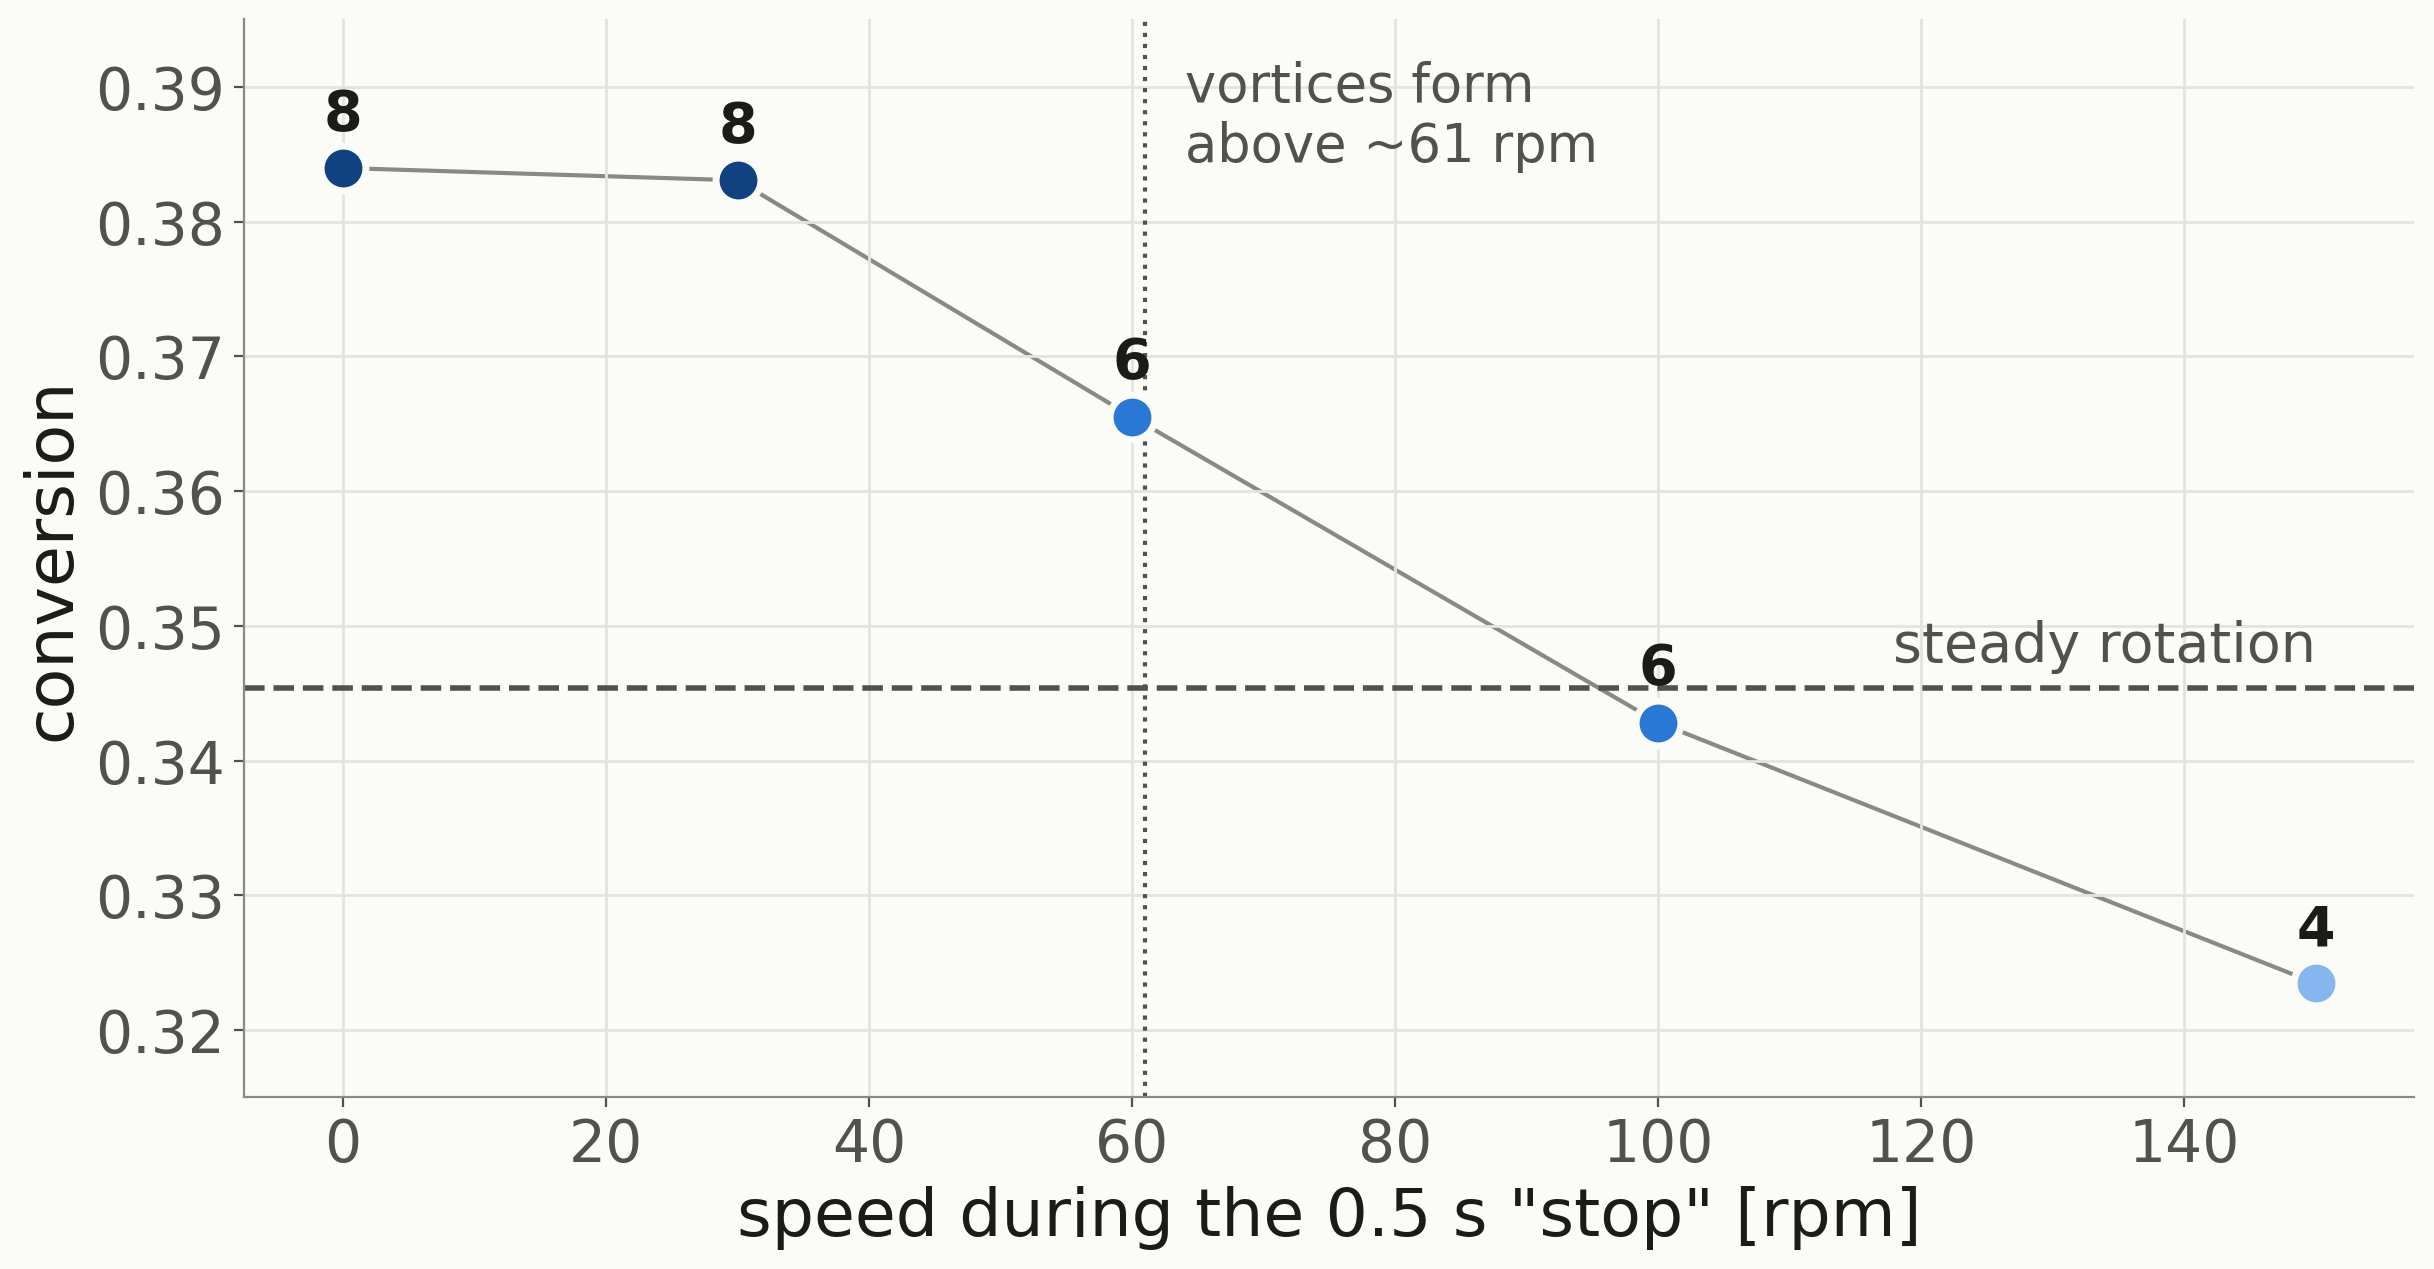
\includegraphics[width=\linewidth,height=0.76\textheight,keepaspectratio]{s_stop_level}
    \end{column}
    \begin{column}{0.30\textwidth}
      Vortices must die first.
    \end{column}
  \end{columns}
\end{frame}
\note{[0:30] Instead of stopping, I slowed the cylinder to 30, 60, 100 or 150 rpm for the same half second. Thirty is as good as a full stop. At 60 rpm, about where vortices start to form, you get six cells instead of eight, and at 100 and above the gain is gone. The vortices really have to die, to about one percent of their energy, before the restart can build a new, finer pattern.}

% ============================================================================
\begin{frame}{Conversion follows the cell count}
  \begin{columns}[c]
    \begin{column}{0.74\textwidth}
      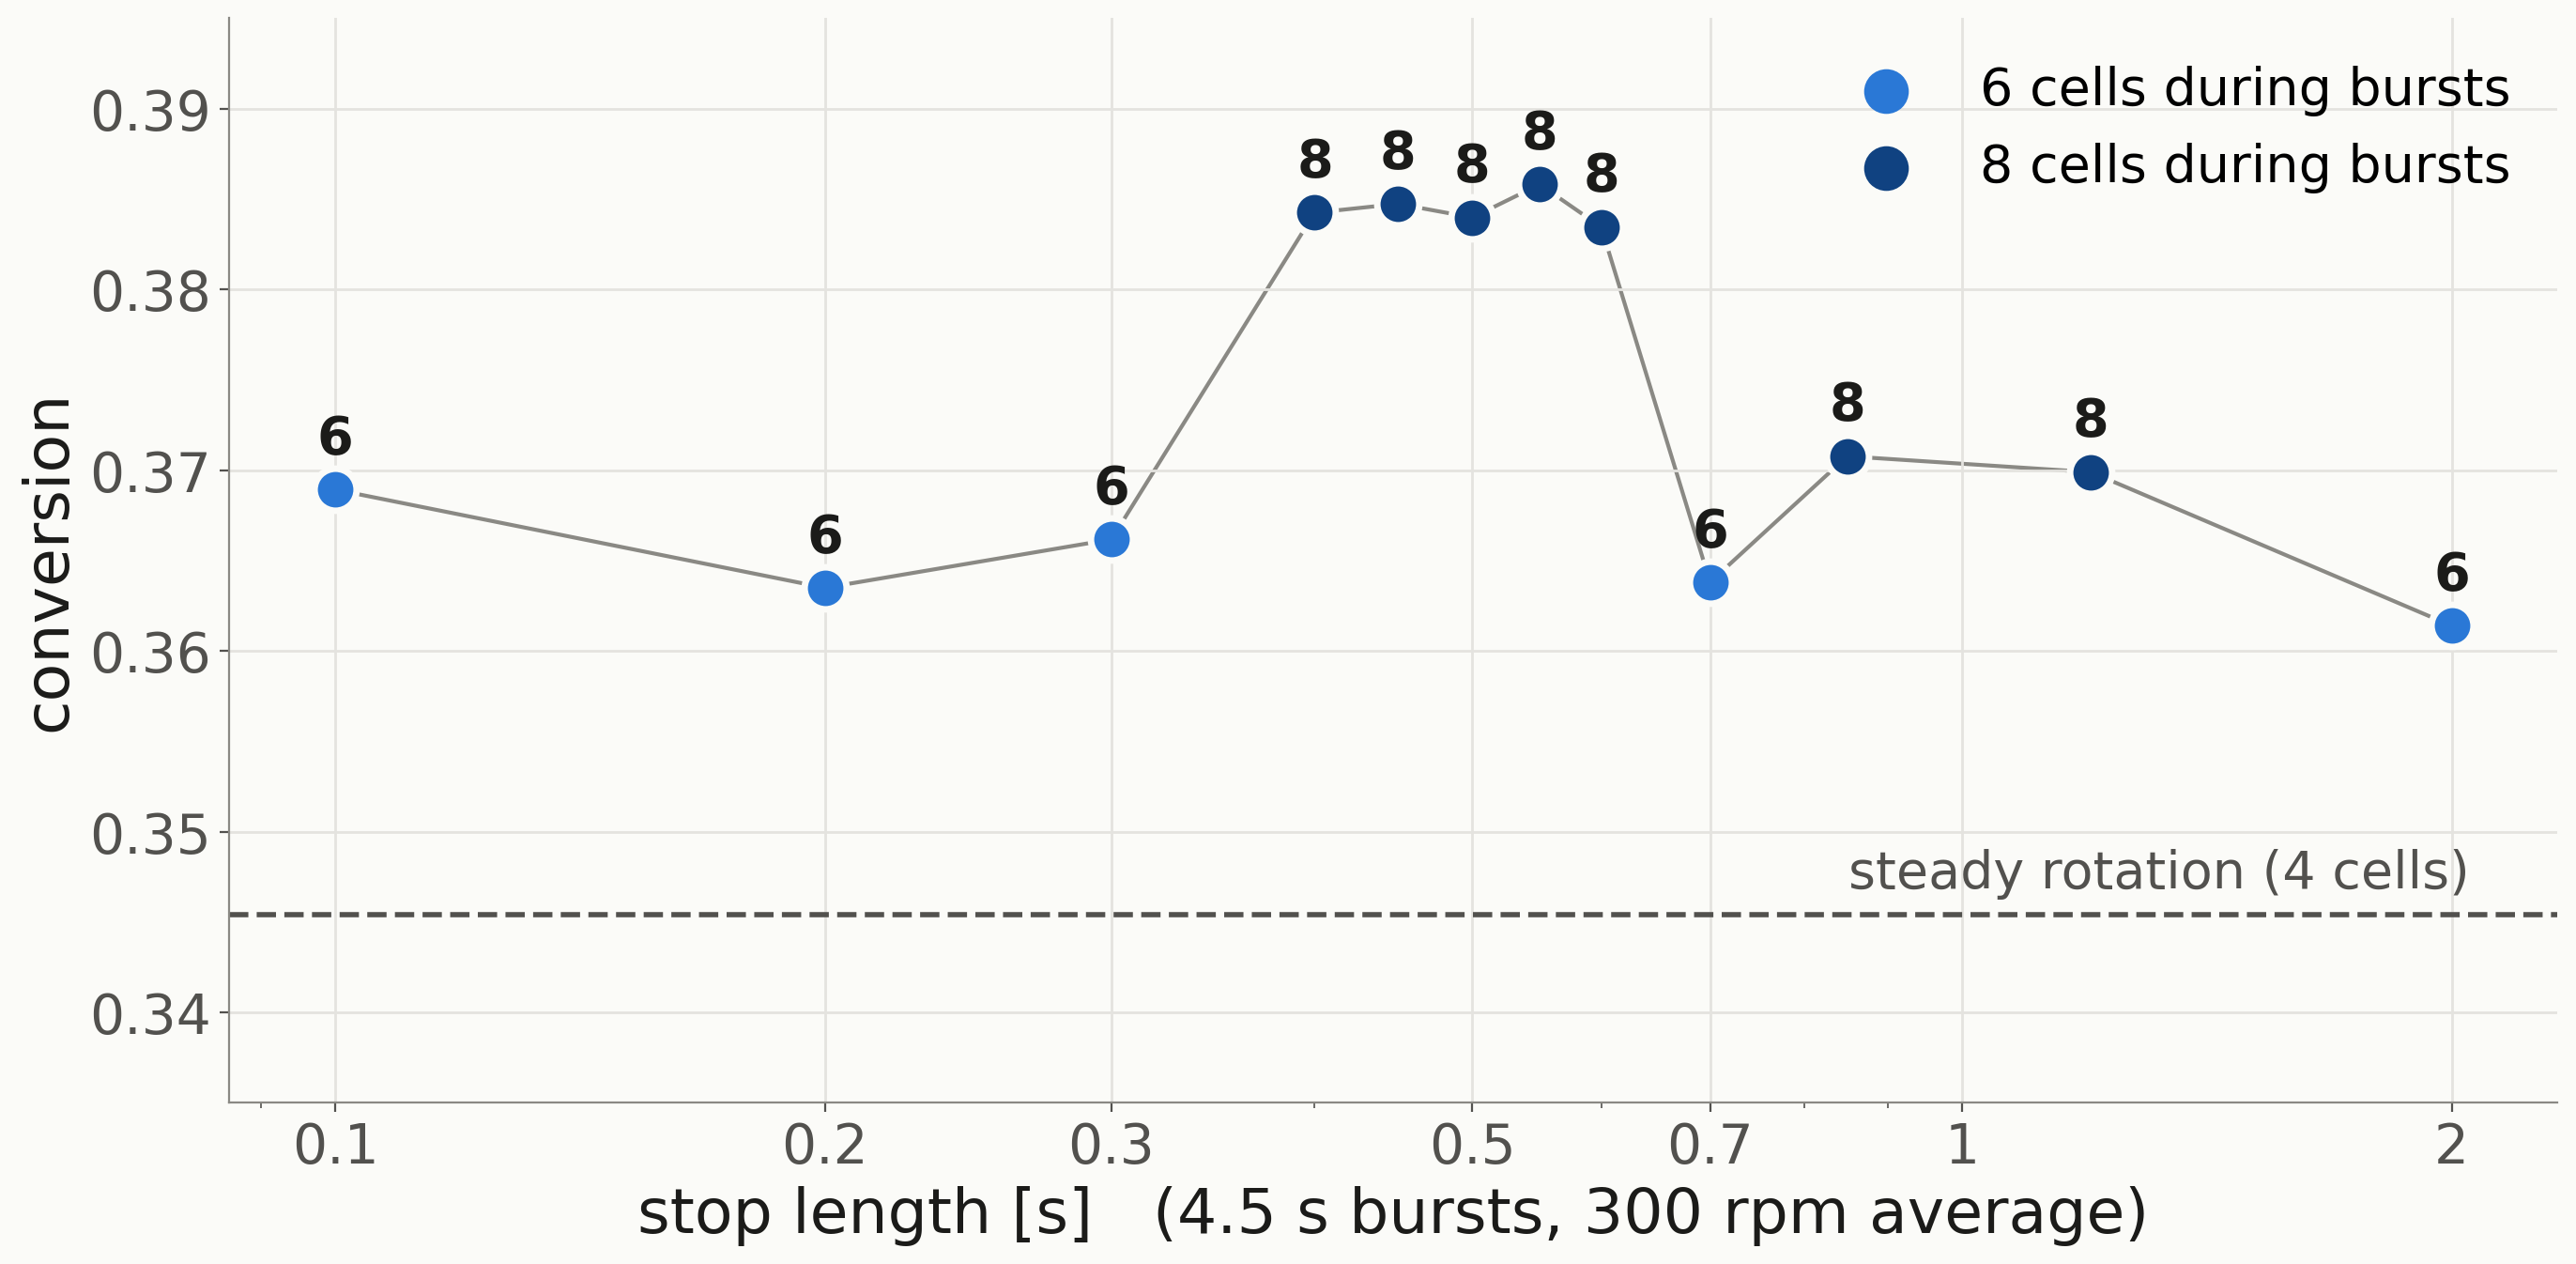
\includegraphics[width=\linewidth,height=0.74\textheight,keepaspectratio]{s_stop_curve_cells}
    \end{column}
    \begin{column}{0.24\textwidth}
      \bignum{+0.04}{conversion in the 8-cell window (0.4--0.6\,s stops)}\par\bigskip
      \bignum{4\,$\to$\,8}{cells, steady vs best pulsing}
    \end{column}
  \end{columns}
\end{frame}
\note{[0:45] Plot conversion against stop length and label each point with its cell count. It isn't a smooth curve with one peak; it's a set of levels. Steady rotation, four cells, at the bottom; six-cell stops in the middle; and the best stops, 0.4 to 0.6 seconds, are exactly the ones whose restart lands in eight cells, about 0.04 above steady rotation. The sudden drop at 0.7 seconds, which looked like a strange cliff in the original search, is just the flow falling back to six cells.}

% ============================================================================
\begin{frame}{Numerical verification}
  \begin{columns}[T]
    \begin{column}{0.58\textwidth}
      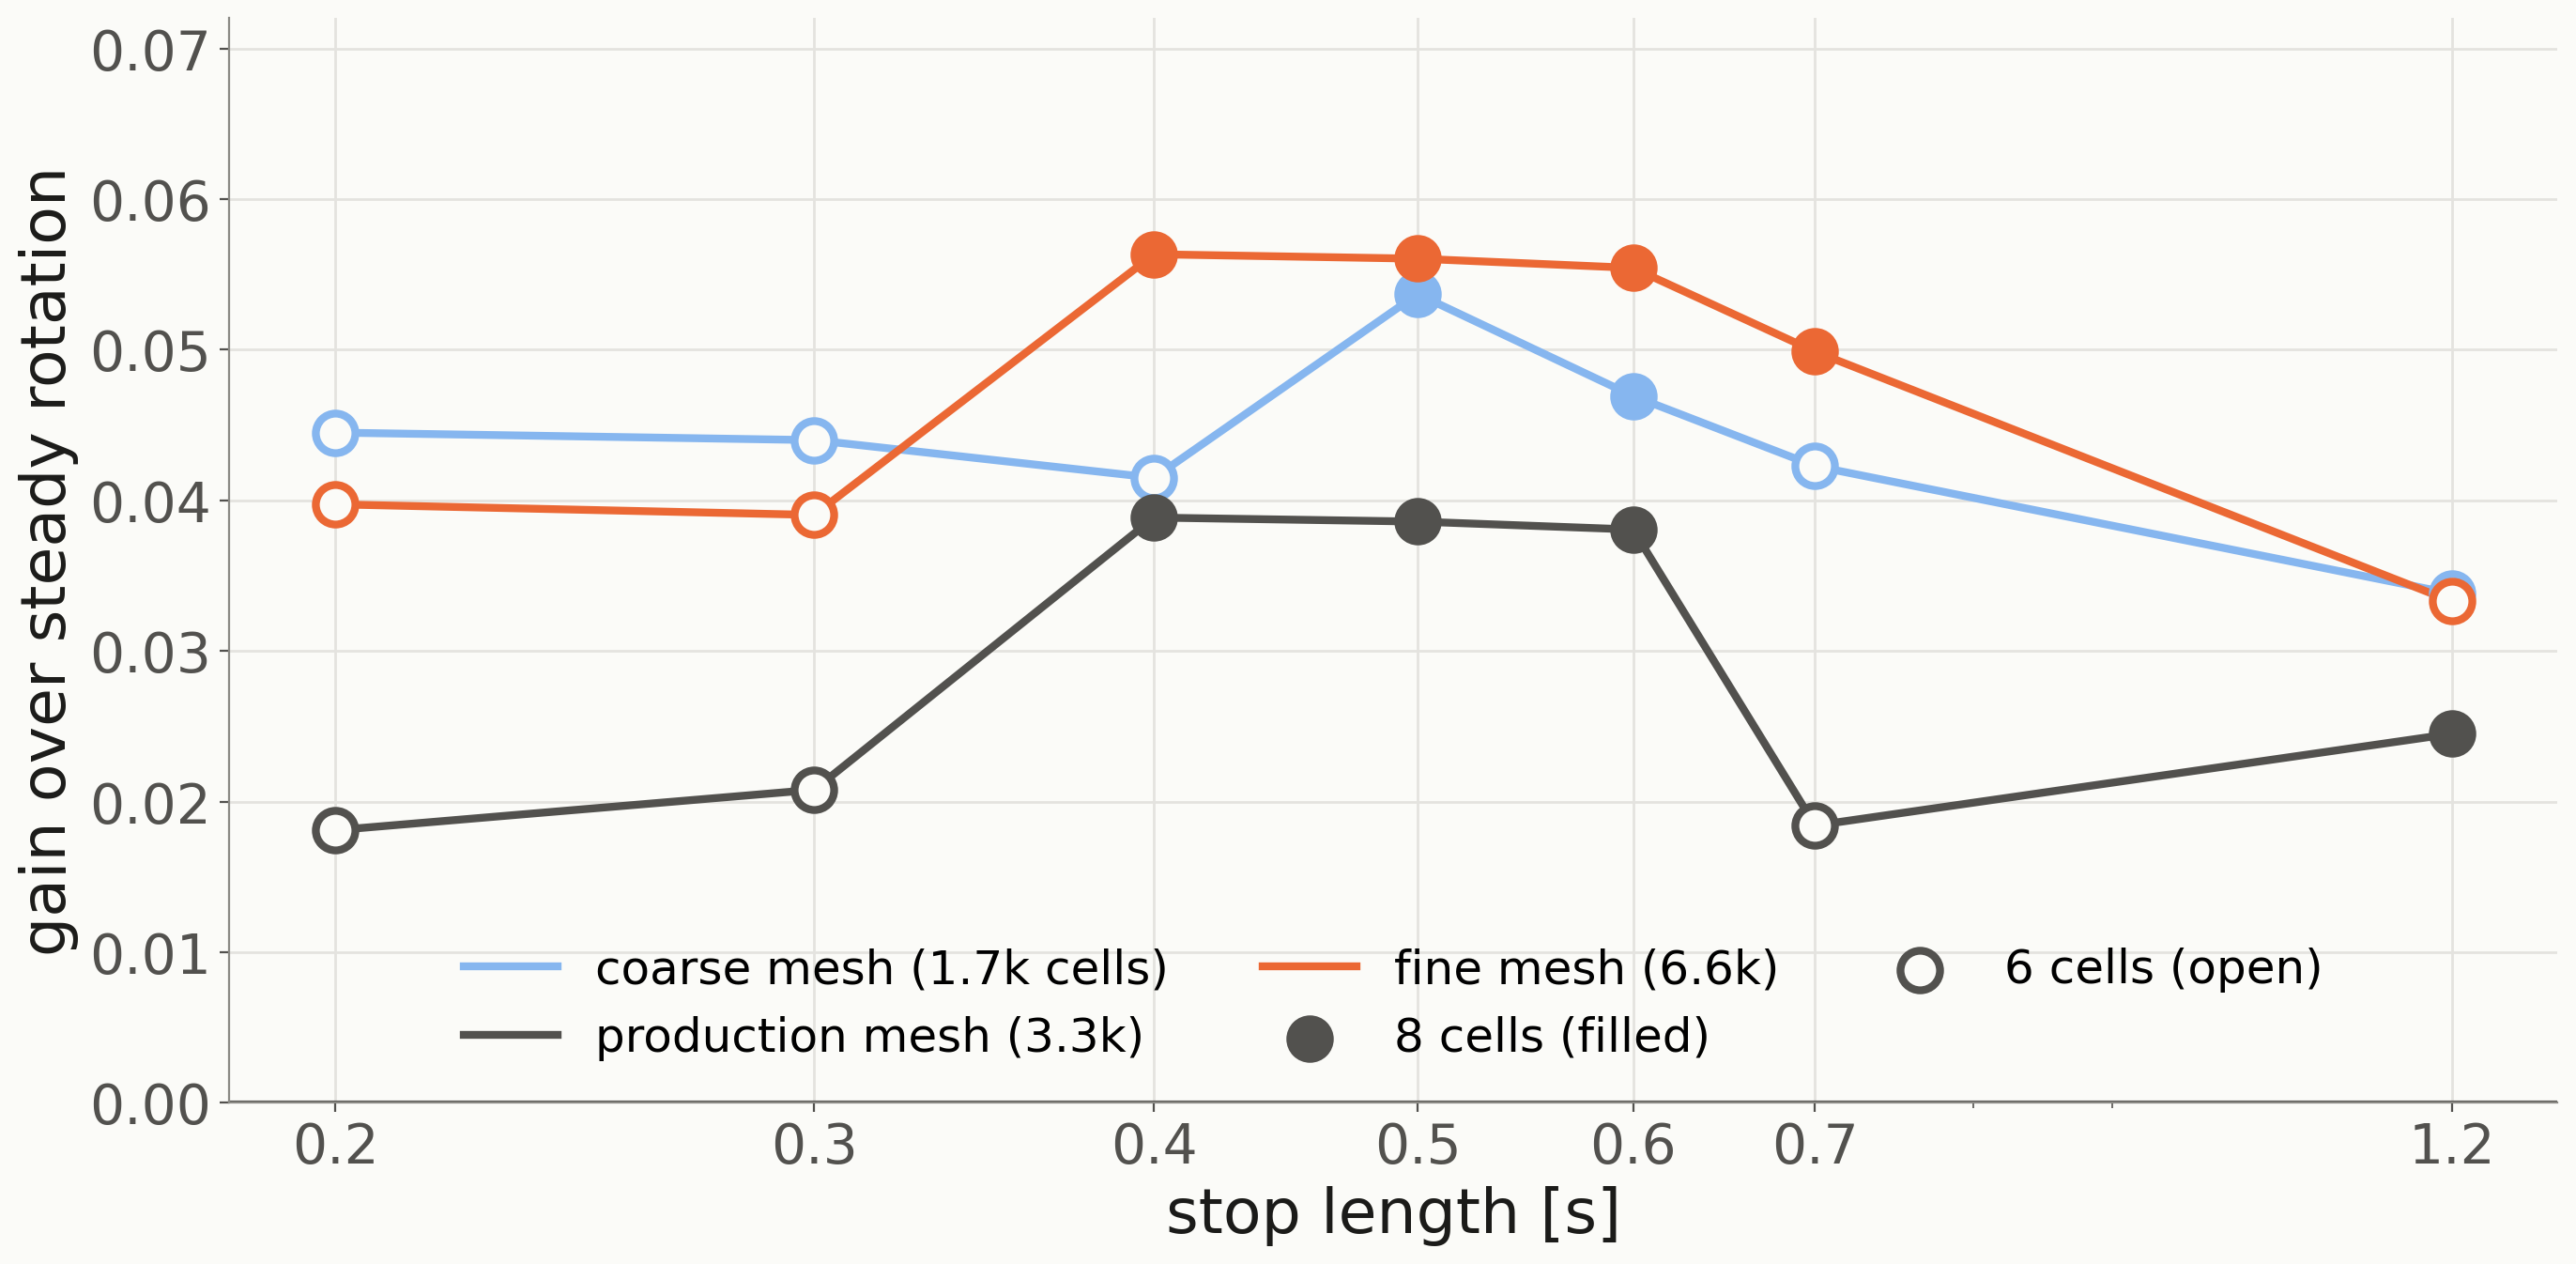
\includegraphics[width=\linewidth,height=0.62\textheight,keepaspectratio]{s_mesh_check}\par
      {\small\color{ink}3 meshes: same cells, gain +0.04 to +0.06}
    \end{column}
    \begin{column}{0.40\textwidth}
      \begin{block}{Checks}
        \begin{itemize}
          \item Half time step: outlet artifact gone
          \item Mass balance: 0.3\%
          \item Replicate noise: 0.002
        \end{itemize}
      \end{block}
    \end{column}
  \end{columns}
\end{frame}
\note{[0:45] For this audience the obvious question is whether it's numerics. I repeated the key runs on a coarser and a finer mesh from the same self-similar family. On all three, steady rotation has four cells, the best stops land in eight, and the gain is four to six hundredths. Halving the time step exposed and removed a spurious jet at the outlet worth about four hundredths of conversion, which is why all these runs use the smaller step. The mass balance closes to a third of a percent and replicate noise is about 0.002. What does move with the mesh is the exact edges of the eight-cell window, by a tenth of a second or two, so I quote ``about half a second''.}

% ============================================================================
\begin{frame}{Three takeaways}
  \begin{enumerate}
    \setlength\itemsep{0.8em}
    \item Brief full stops beat steady rotation and the published recipe.
    \item RL learns near-optimal control: matches 220-run optimization, transfers $5\times$ taller.
    \item Mechanism: restarts select more Taylor cells (8 vs 4); stops must repeat.
  \end{enumerate}
  \vfill
  {\small\color{ink}\textbf{Next:} messy conditions (feed, fluid drift) $\to$ feedback control; 3D check.\par\smallskip
  \textbf{Limits:} 2D axisymmetric; $\mathrm{Sc}=1075$.}
\end{frame}
\note{[0:45] One: brief full stops beat steady rotation at the same power, and beat the published recipe. Two: the RL pipeline learns near-optimal control from simulation alone. With no physics given, it matched an independent 220-run optimization, which is how we know it found the right answer, and it carried over to a reactor five times taller. Three: the optimum exploits multistability. Each restart selects a state with more cells that transports reactant faster, and because that state decays back under steady forcing, the stops have to repeat. This problem turned out to be simple: steady conditions, one best waveform, so a static optimizer can solve it too, and RL tying it is what you'd expect. The next step is to make it messy: changing feed rates and drifting fluid properties, where no fixed waveform stays right and a feedback policy should pull ahead. The main limit is the 2D model, so the mechanism is still a hypothesis for real 3D flow. Thank you, happy to take questions.}

% ============================================================================
\appendix
\begin{frame}{Backup: best fixed waveform vs the RL policy}
  \centering
  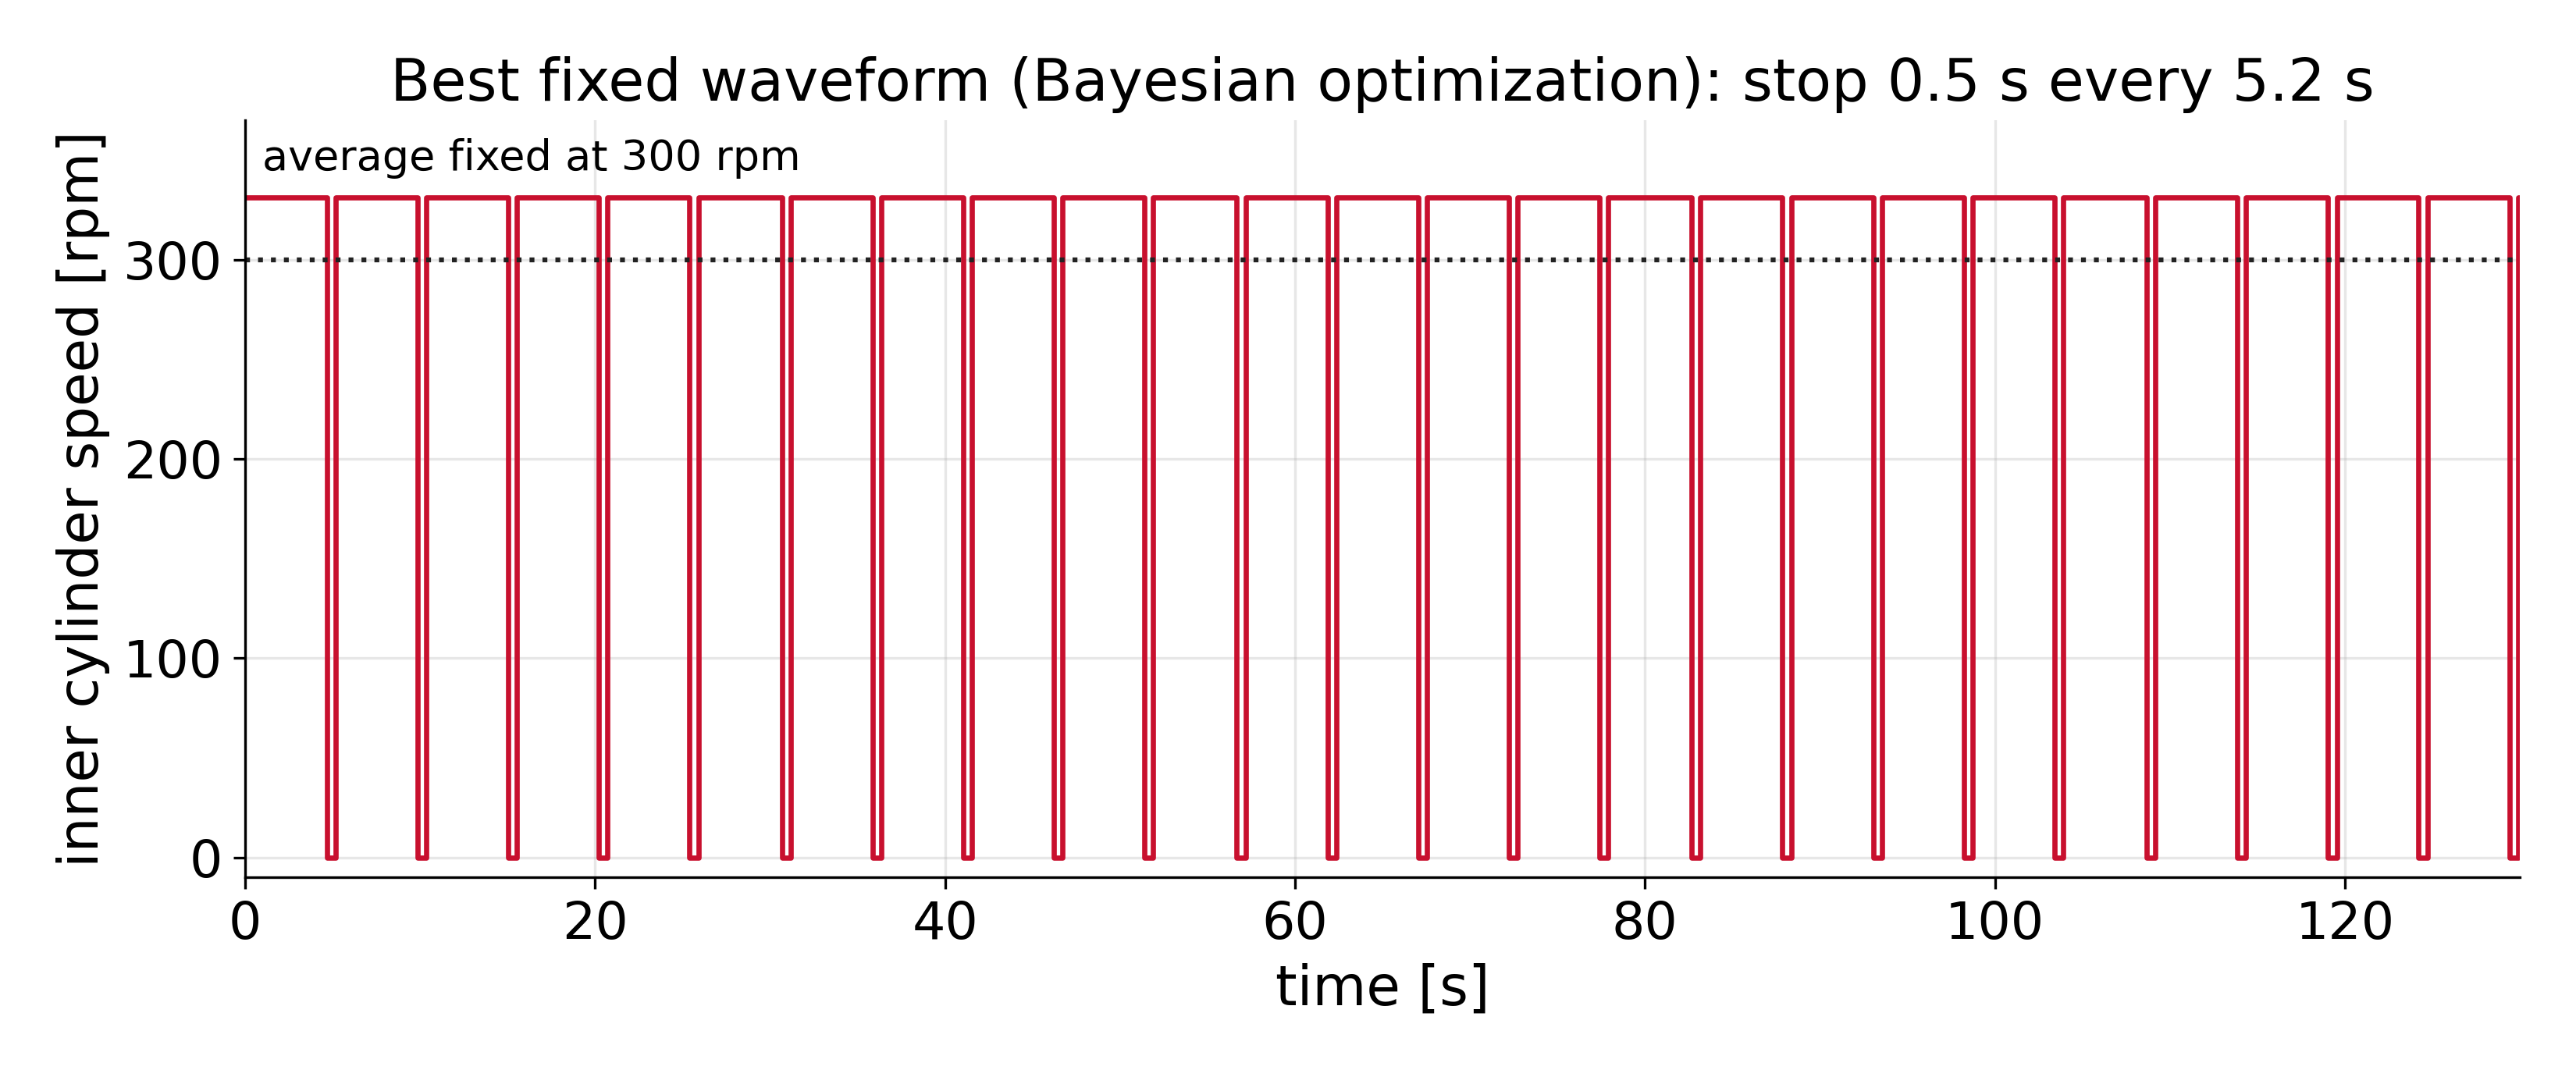
\includegraphics[width=0.86\linewidth,height=0.40\textheight,keepaspectratio]{bo_best_waveform}\par\smallskip
  \includegraphics[width=0.86\linewidth,height=0.40\textheight,keepaspectratio]{fig4_learned_waveform}
\end{frame}
\note{[Backup] Top: the best fixed waveform from the 220-run Bayesian optimization, stop half a second every five seconds, peak about 330 rpm. Bottom: what the RL policy chose. Same idea, brief full stops at high duty, but RL's stops are shorter, mostly a tenth to four tenths of a second, which mostly lands in the six-cell state and costs it one to two hundredths of conversion.}

% ============================================================================
\begin{frame}{Backup: why 0.5\,s? Two time scales, two predictions}
  \begin{columns}[T]
    \begin{column}{0.48\textwidth}
      \begin{block}{Swirl decay}
        \[ \tau = \frac{d^2}{\pi^2 \nu} \approx 0.4\ \mathrm{s} \]
        Slowest decay mode of momentum diffusion across the gap. Predicts best stop $\propto \nu^{-1}$.
      \end{block}
    \end{column}
    \begin{column}{0.48\textwidth}
      \begin{block}{Wall layer}
        \[ \tau = \frac{\delta^2}{D} \approx 0.8\ \mathrm{s} \]
        Regrowth of the depleted layer at the wall. At fixed $D$, predicts best stop $\propto \nu^{0.3}$ to $\nu^{0.7}$.
      \end{block}
    \end{column}
  \end{columns}
  \bigskip
  \takeaway{\textbf{Test:} vary $\nu$ at fixed $D$ and fit best stop $\propto \nu^{a}$. The sign of $a$ decides.}
\end{frame}
\note{[Backup] If asked whether a simple time scale explains the stop length: why half a second? Two time scales sit near it. One is the decay of the swirl: the slowest mode of momentum diffusion across a gap of width d decays on d squared over pi squared nu, about 0.4 seconds. The other is the time for the reactant-depleted layer at the wall to regrow, delta squared over D, about 0.8 seconds. They scale differently with viscosity. Holding the diffusivity fixed, the swirl clock predicts the best stop goes like nu to the minus one; the wall-layer clock predicts a positive power, about 0.3 to 0.7. So I varied the viscosity, fit an exponent, and decided in advance that its sign would pick the winner.}

% ============================================================================
\begin{frame}{Backup: neither guess sets the best stop}
  The swirl decays exactly as theory says (left), but the best stop follows neither prediction (right).\par\medskip
  \centering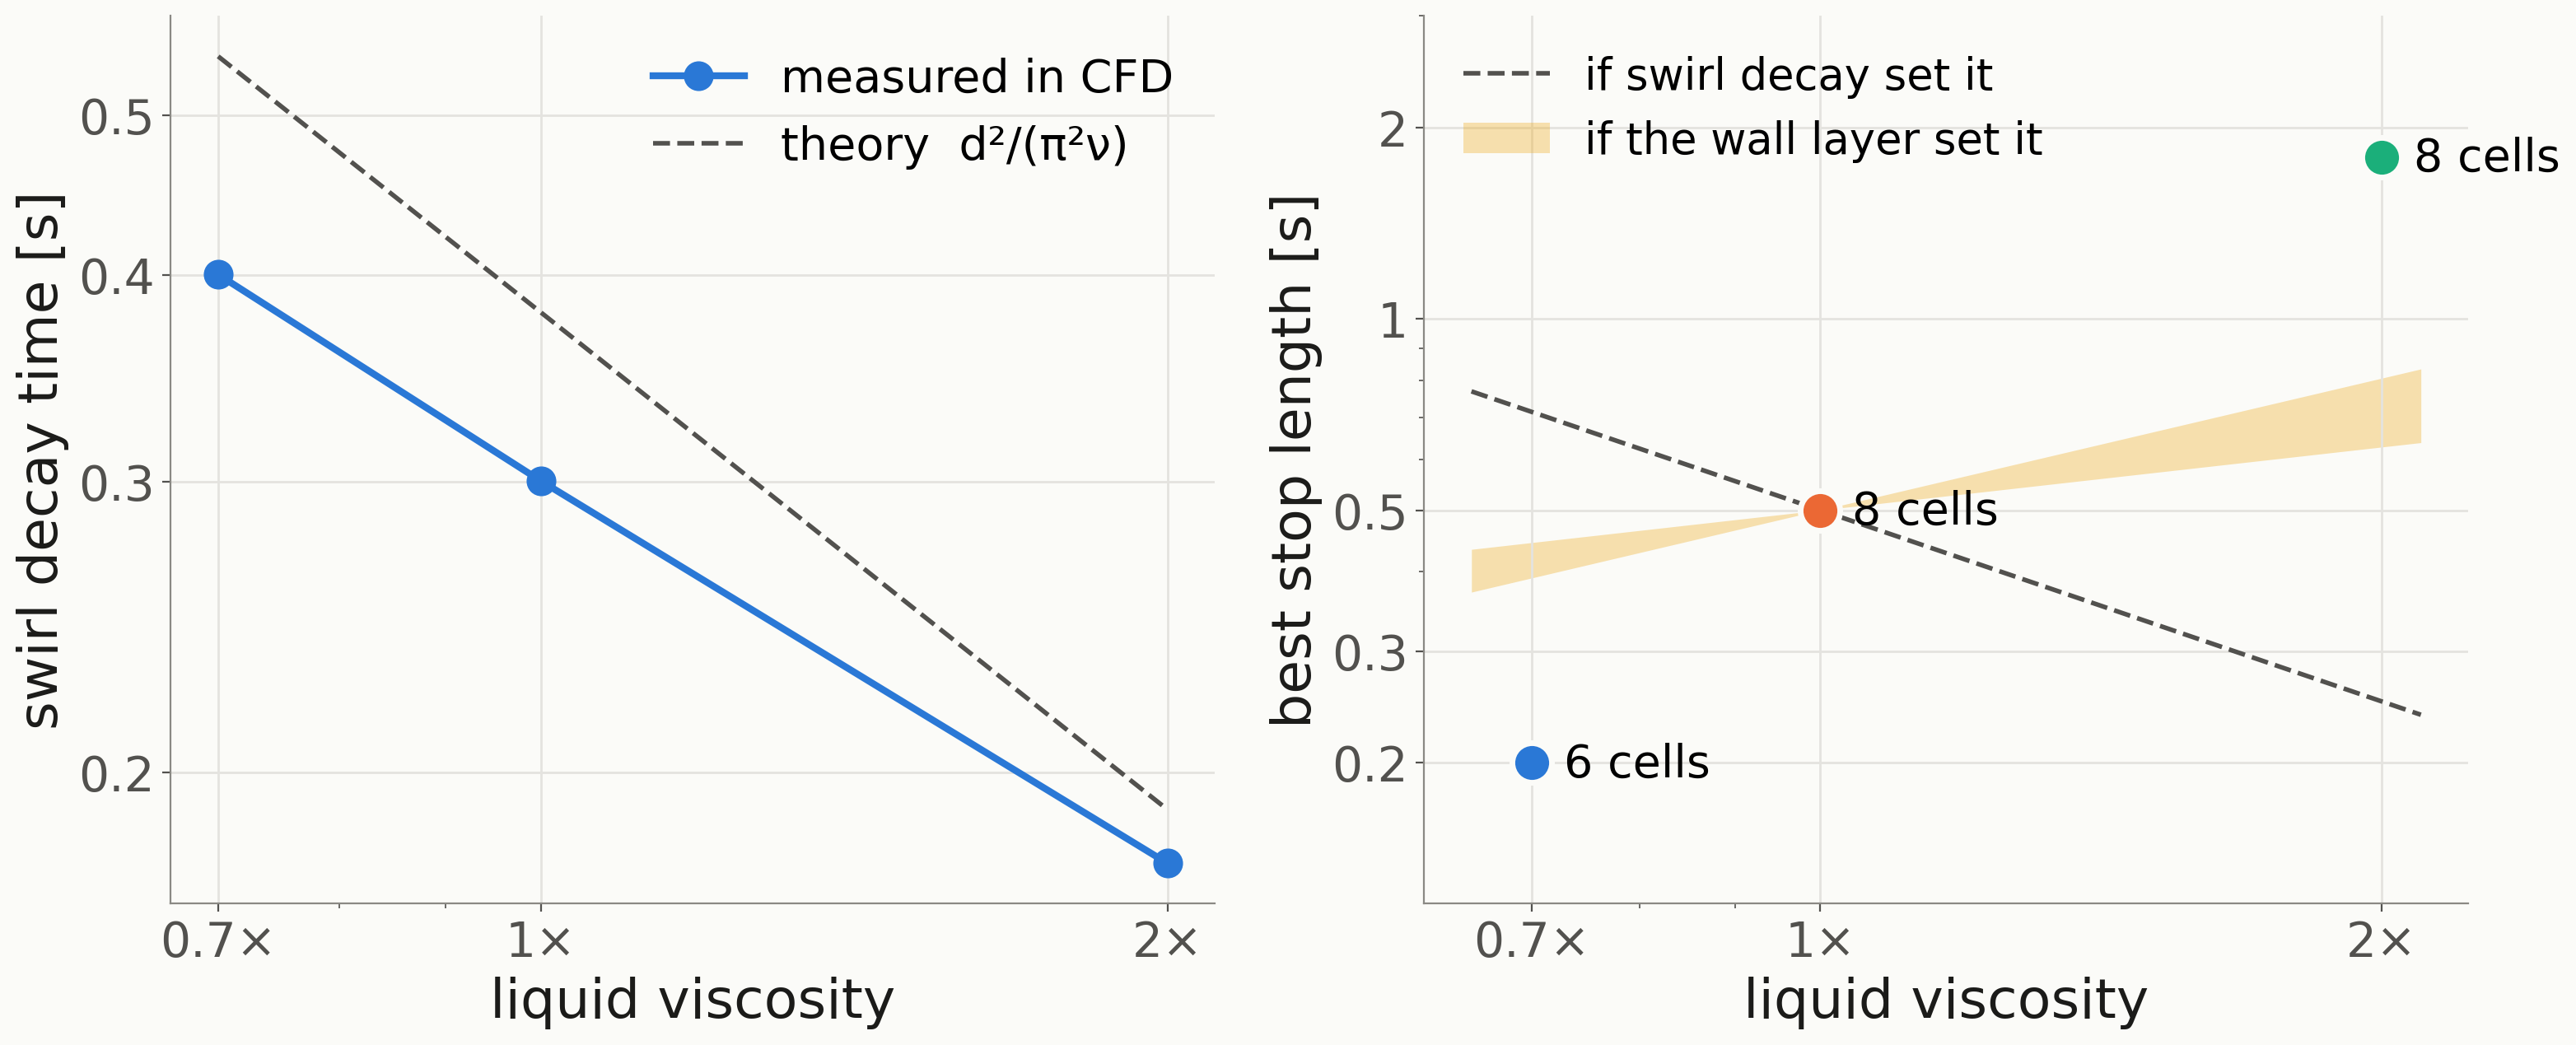
\includegraphics[width=\linewidth,height=0.66\textheight,keepaspectratio]{s_clocks}
\end{frame}
\note{[Backup] On the left, the swirl decays exactly as the eigenmode estimate says, one over viscosity. On the right, the best stop follows neither prediction; a formal exponent fit isn't even meaningful, because the optimum jumps rather than drifting. The labels, six cells and eight cells, are the clue.}


\begin{frame}{Backup: the gain is a higher plateau, not a restart spike}
  \centering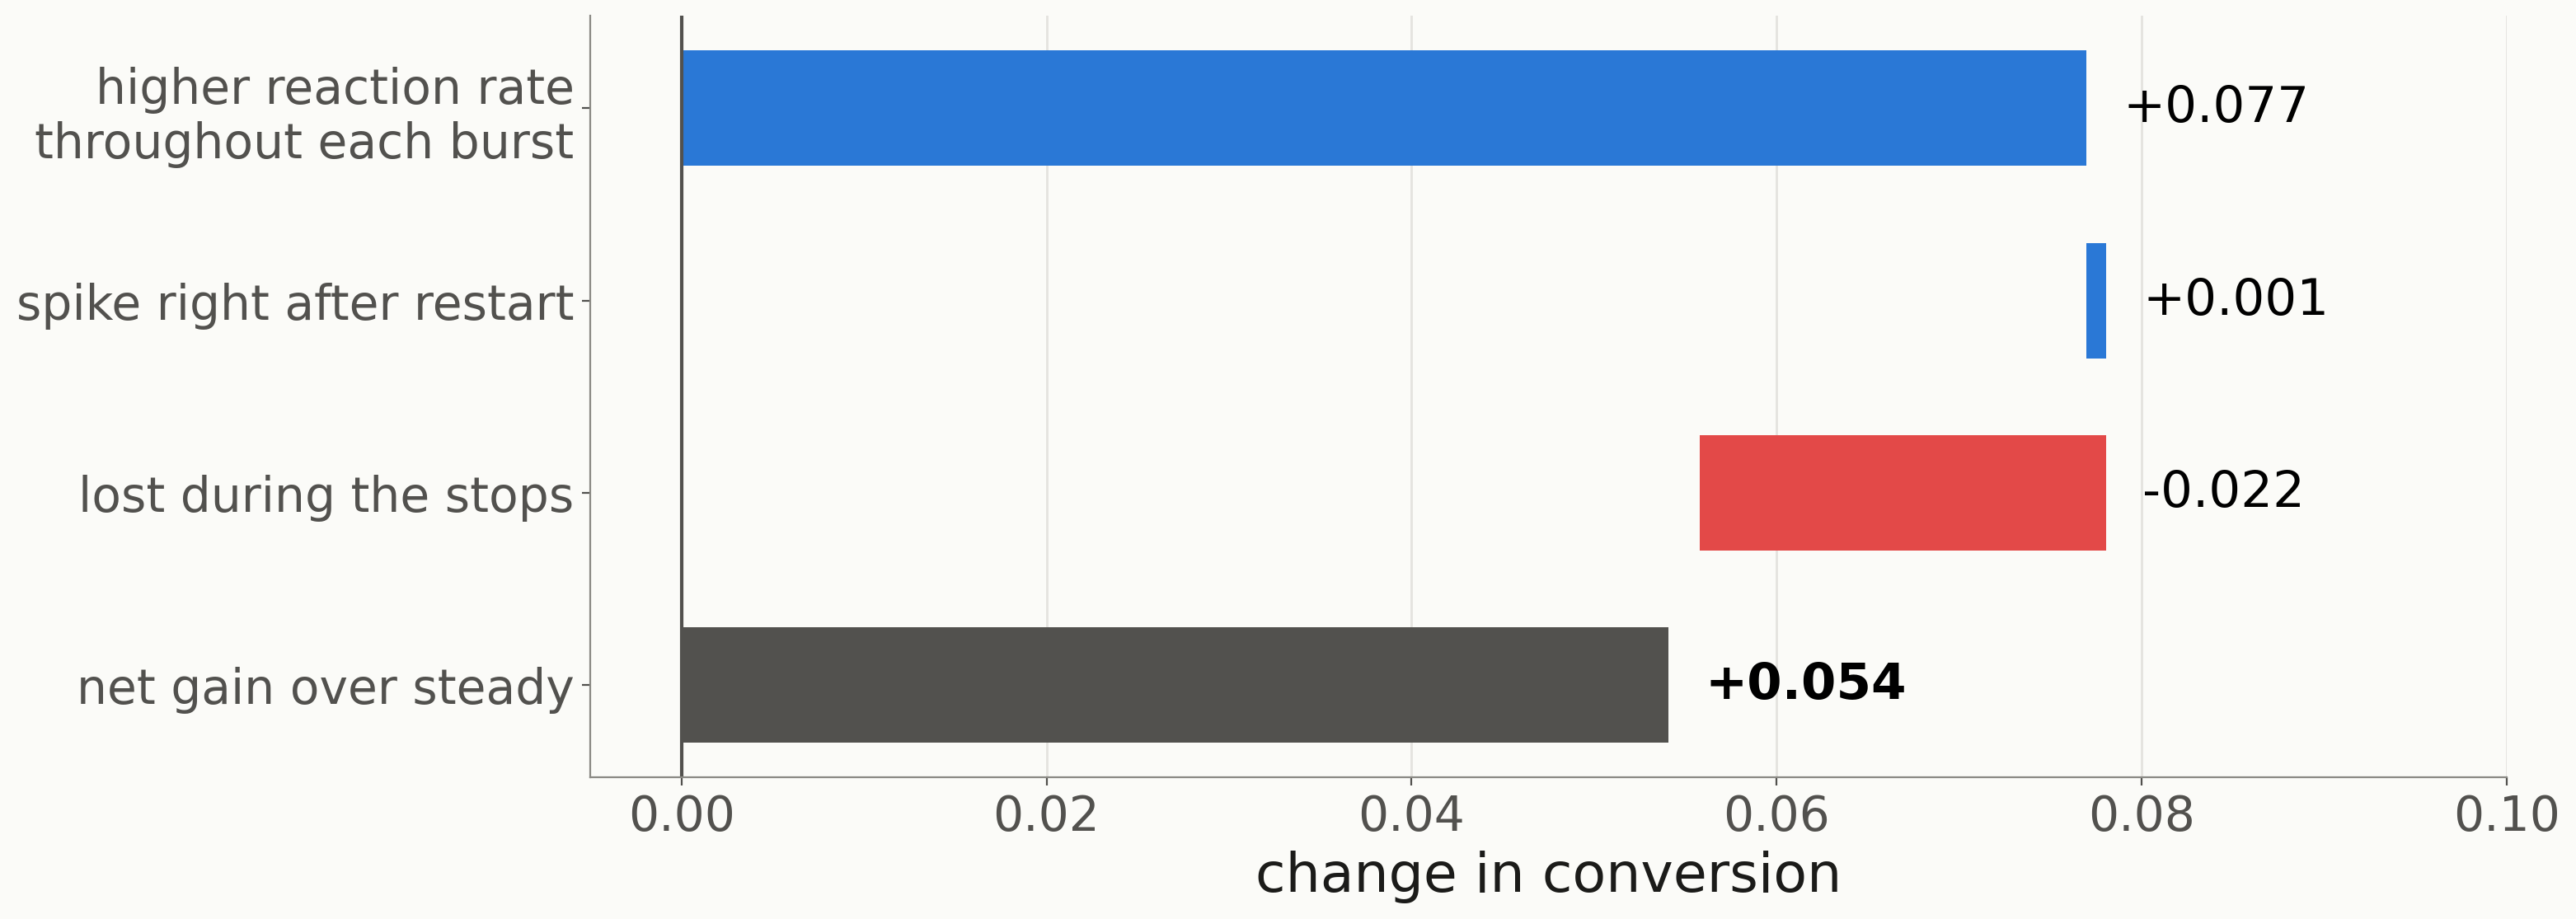
\includegraphics[width=\linewidth,height=0.62\textheight,keepaspectratio]{s_gain_breakdown}\par\smallskip
  \raggedright{\small\color{ink}From the wall-reaction traces of the best waveform's original run (wall-flux budget, last 26\,s).}
\end{frame}
\note{[Backup] If asked whether this is just a restart spike (``film renewal''): no. Splitting the gain over steady rotation: +0.077 from the reaction rate staying higher through the whole burst, only +0.001 from the spike right after restart, and $-0.022$ lost while stopped. The parts sum to 0.056 against the measured 0.054; the difference comes from how the burst plateau is defined.}

\begin{frame}{Backup: gain needs cells added over steady rotation}
  \begin{columns}[c]
    \begin{column}{0.64\textwidth}
      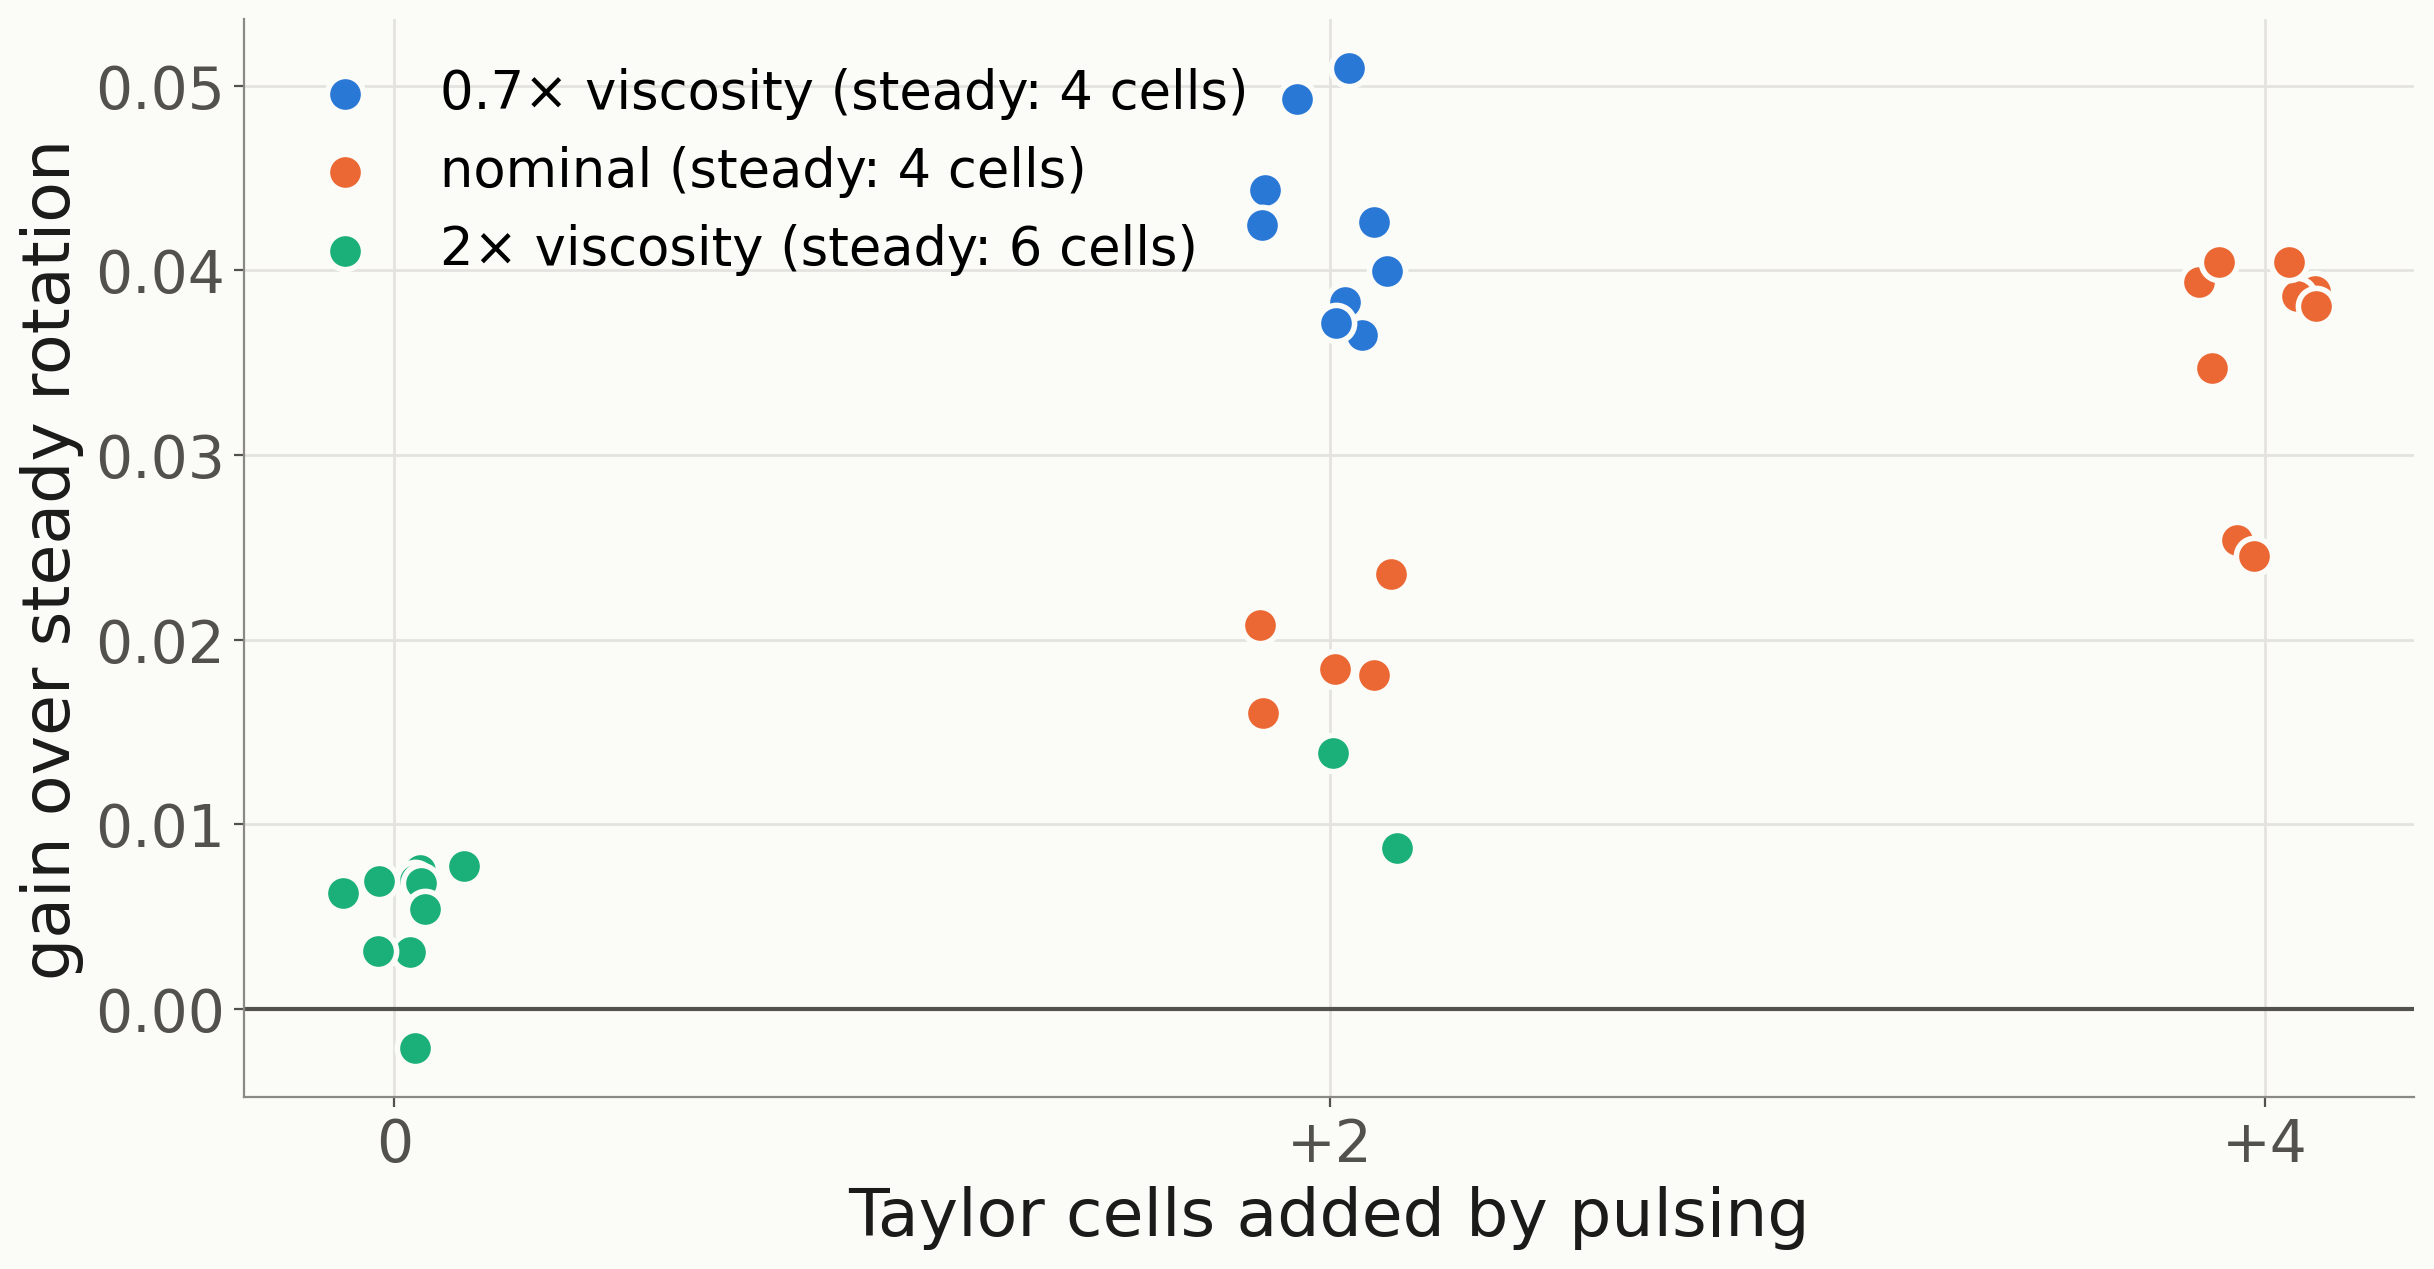
\includegraphics[width=\linewidth,height=0.72\textheight,keepaspectratio]{s_cells_added_gain}
    \end{column}
    \begin{column}{0.34\textwidth}
      At $2\times$ viscosity, steady rotation already holds 6 cells. Most pulses add none, and the gain shrinks to about +0.01.
    \end{column}
  \end{columns}
\end{frame}
\note{[Backup] Every pulsed run from the viscosity sweep, by how many cells pulsing adds over steady rotation at that viscosity. Runs that add no cells gain almost nothing; runs that add two or four gain up to five hundredths. At twice the viscosity steady rotation already has six cells, so most pulses add none. The size of the gain also depends on viscosity, so it isn't one universal curve.}

\begin{frame}{Backup: electrical power model}
  \begin{columns}[T]
    \begin{column}{0.58\textwidth}
      \begin{block}{L\'opez-Guajardo et al.\ (2024), \S3.4, Eqs.\ 18--23}
        {\small
        \[ T_{\mathrm{mot}} = \underbrace{J_{\mathrm{tot}}\,\dot\omega}_{\text{inertia}}
           + \underbrace{T_0\,\mathrm{sign}(\omega)}_{\text{bearings}}
           + \underbrace{\beta_2\,\omega^2\,\mathrm{sign}(\omega) + \beta_1\,\omega}_{\text{drag}} \]
        \[ i_{\mathrm{mot}} = \frac{T_{\mathrm{mot}}}{K_t}, \qquad
           e_{\mathrm{mot}} = L\,\frac{di_{\mathrm{mot}}}{dt} + R\,i_{\mathrm{mot}} + K_e\,\omega \]
        \[ P_{\mathrm{mot}} = e_{\mathrm{mot}}\, i_{\mathrm{mot}}, \qquad
           P_e = \begin{cases} P_{\mathrm{mot}}/\eta, & P_{\mathrm{mot}} \ge 0 \\ P_{\mathrm{mot}}\,\eta, & P_{\mathrm{mot}} < 0 \end{cases} \]}
      \end{block}
      {\small\color{ink}Evaluated on the commanded $\omega(t)$; reward uses $\overline{P_e}/P_{\max}$, $P_{\max} = 31.94$\,W (2500 rpm).}
    \end{column}
    \begin{column}{0.40\textwidth}
      {\small
      \begin{tabular*}{\linewidth}{@{}l@{\extracolsep{\fill}}r@{}}
        \toprule
        $J_{\mathrm{tot}}$ & $1.66\times10^{-4}$ kg\,m$^2$ \\
        $T_0$ & 0.1 N\,m \\
        $\beta_2$ & $7.19\times10^{-8}$ N\,m\,s$^2$ \\
        $\beta_1$ & $1.51\times10^{-5}$ N\,m\,s \\
        $K_t = K_e$ & 93.1 mN\,m/A \\
        $L$, \ $R$ & 0.28 mH, \ 0.178\,$\Omega$ \\
        $\eta$ & 0.90 \\ \bottomrule
      \end{tabular*}}\par\medskip
      {\small\color{ink}At 300 rpm the bearing term alone is $\approx$ 3.5 of the 3.7\,W, so power is set by the mean speed.}
    \end{column}
  \end{columns}
\end{frame}
\note{[Backup] The power model is the one L\'opez-Guajardo and colleagues used, Section 3.4 of their paper: motor torque from inertia, bearing friction and a quadratic drag fit; current from the torque constant; voltage from the armature circuit; electrical power with a 90 percent controller efficiency, and regeneration when braking. We evaluate it on the commanded speed and normalize by the power at 2500 rpm, 31.94 watts. At 300 rpm almost all of the 3.7 watts is bearing friction, which depends only on speed, so fixing the mean speed fixes the power, whatever the waveform's shape.}

\end{document}
"   (x2)
%                                                    -> talk_notes.pdf (slides + speaker notes)
% Figures: ../figures (make_slide_figures.py) and ../../poster_2026-10-02.
\documentclass[aspectratio=169,11pt]{beamer}
\usetheme{default}
\usepackage{lmodern}
\setbeamertemplate{navigation symbols}{}
\setbeamertemplate{blocks}[rounded][shadow=false]
\setbeamertemplate{footline}[frame number]
\setbeamertemplate{itemize items}[circle]
\usepackage[utf8]{inputenc}
\usepackage[T1]{fontenc}
\usepackage{amsmath,amssymb,bm}
\usepackage{booktabs}
\usepackage{tikz}
\usetikzlibrary{arrows.meta}
\graphicspath{{../figures/}{../../poster_2026-10-02/}{../../}}

\ifdefined\withnotes
  \setbeameroption{show notes}
  \setbeamertemplate{note page}[plain]
\fi

% ---- University of Houston palette (from the UH URD template) ---------------
% UH Red #C8102E, Brick #960C22, Slate #54585A; logos cut from the template's banner.
\definecolor{uhred}{HTML}{C8102E}
\definecolor{uhbrick}{HTML}{960C22}
\definecolor{uhslate}{HTML}{54585A}
\definecolor{navy}{HTML}{231F20}     % primary text (near-black)
\definecolor{ink}{HTML}{54585A}      % secondary text (UH slate)
\definecolor{accent}{HTML}{C8102E}
\definecolor{accentdk}{HTML}{960C22}
\definecolor{paper}{HTML}{FBFBF8}    % matches the figure backgrounds
\definecolor{card}{HTML}{F1F0EE}
\definecolor{vblue}{HTML}{1C5CAB}
\setbeamercolor{normal text}{fg=navy,bg=paper}
\setbeamercolor{frametitle}{fg=white,bg=uhred}
\setbeamercolor{alerted text}{fg=uhred}
\setbeamercolor{block title}{fg=uhbrick,bg=card}
\setbeamercolor{block body}{fg=ink,bg=card}
\setbeamercolor{structure}{fg=uhred}
\setbeamercolor{page number in head/foot}{fg=uhslate}
\setbeamerfont{block title}{size=\small,series=\bfseries}
\setbeamertemplate{frametitle}{%
  \nointerlineskip%
  \begin{beamercolorbox}[wd=\paperwidth,ht=7.5mm,dp=2.8mm,leftskip=4.5mm,rightskip=3.5mm]{frametitle}%
    \usebeamerfont{frametitle}\insertframetitle\hfill\raisebox{-1.7mm}{
\includegraphics[height=6.2mm]{uh/uh_mark_white}}%
  \end{beamercolorbox}%
  \vspace{1mm}}

\newcommand{\takeaway}[1]{\par\smallskip{\color{ink}#1}\par}
\newcommand{\bignum}[2]{{\usebeamerfont{title}\color{navy}\LARGE\bfseries #1}\\[-1pt]{\small\color{ink}#2}}

\title{Brief stops, more vortices}
\subtitle{Deep reinforcement learning discovers transferable control strategies for catalytic-wall Taylor--Couette reactors}
\author{Isaiah N.\ Bascom\inst{1} \and Min Wang\inst{1} \and Yuhe Wang\inst{2}}
\institute{\inst{1}Department of Mathematics, University of Houston, Houston, Texas \and \inst{2}Institute for Scientific Computation, Texas A\&M University, College Station, Texas}
\date{GCURS 2026 \textbullet\ Computational \& Applied Mathematics}

\begin{document}

% ============================================================================
\begin{frame}[plain]
  \begin{tikzpicture}[remember picture,overlay]
    \fill[uhred] (current page.north west) rectangle ([yshift=-15mm]current page.north east);
    \node[anchor=west] at ([xshift=6mm,yshift=-7.5mm]current page.north west) {
\includegraphics[height=9.5mm]{uh/uh_mark_white}};
    \node[anchor=east] at ([xshift=-6mm,yshift=-7.5mm]current page.north east) {
\includegraphics[height=10.5mm]{uh/uh_wordmark_white}};
    \node[anchor=center, text=white, font=\scriptsize\bfseries] at ([yshift=-7.5mm]current page.north) {GCURS 2026 \textbullet\ COMPUTATIONAL \& APPLIED MATHEMATICS};
    \node[anchor=north west, text width=148mm, align=left, inner sep=0pt, text=navy, font=\usebeamerfont{title}\huge\bfseries]
      at ([xshift=6mm,yshift=-20mm]current page.north west) {Brief stops, more vortices};
    \node[anchor=north west, inner sep=0pt, text=ink]
      at ([xshift=6mm,yshift=-31mm]current page.north west) {\resizebox{148mm}{!}{Deep reinforcement learning discovers transferable control strategies for catalytic-wall Taylor--Couette reactors}};
    \node[anchor=north, inner sep=0pt] at ([yshift=-40mm]current page.north)
      {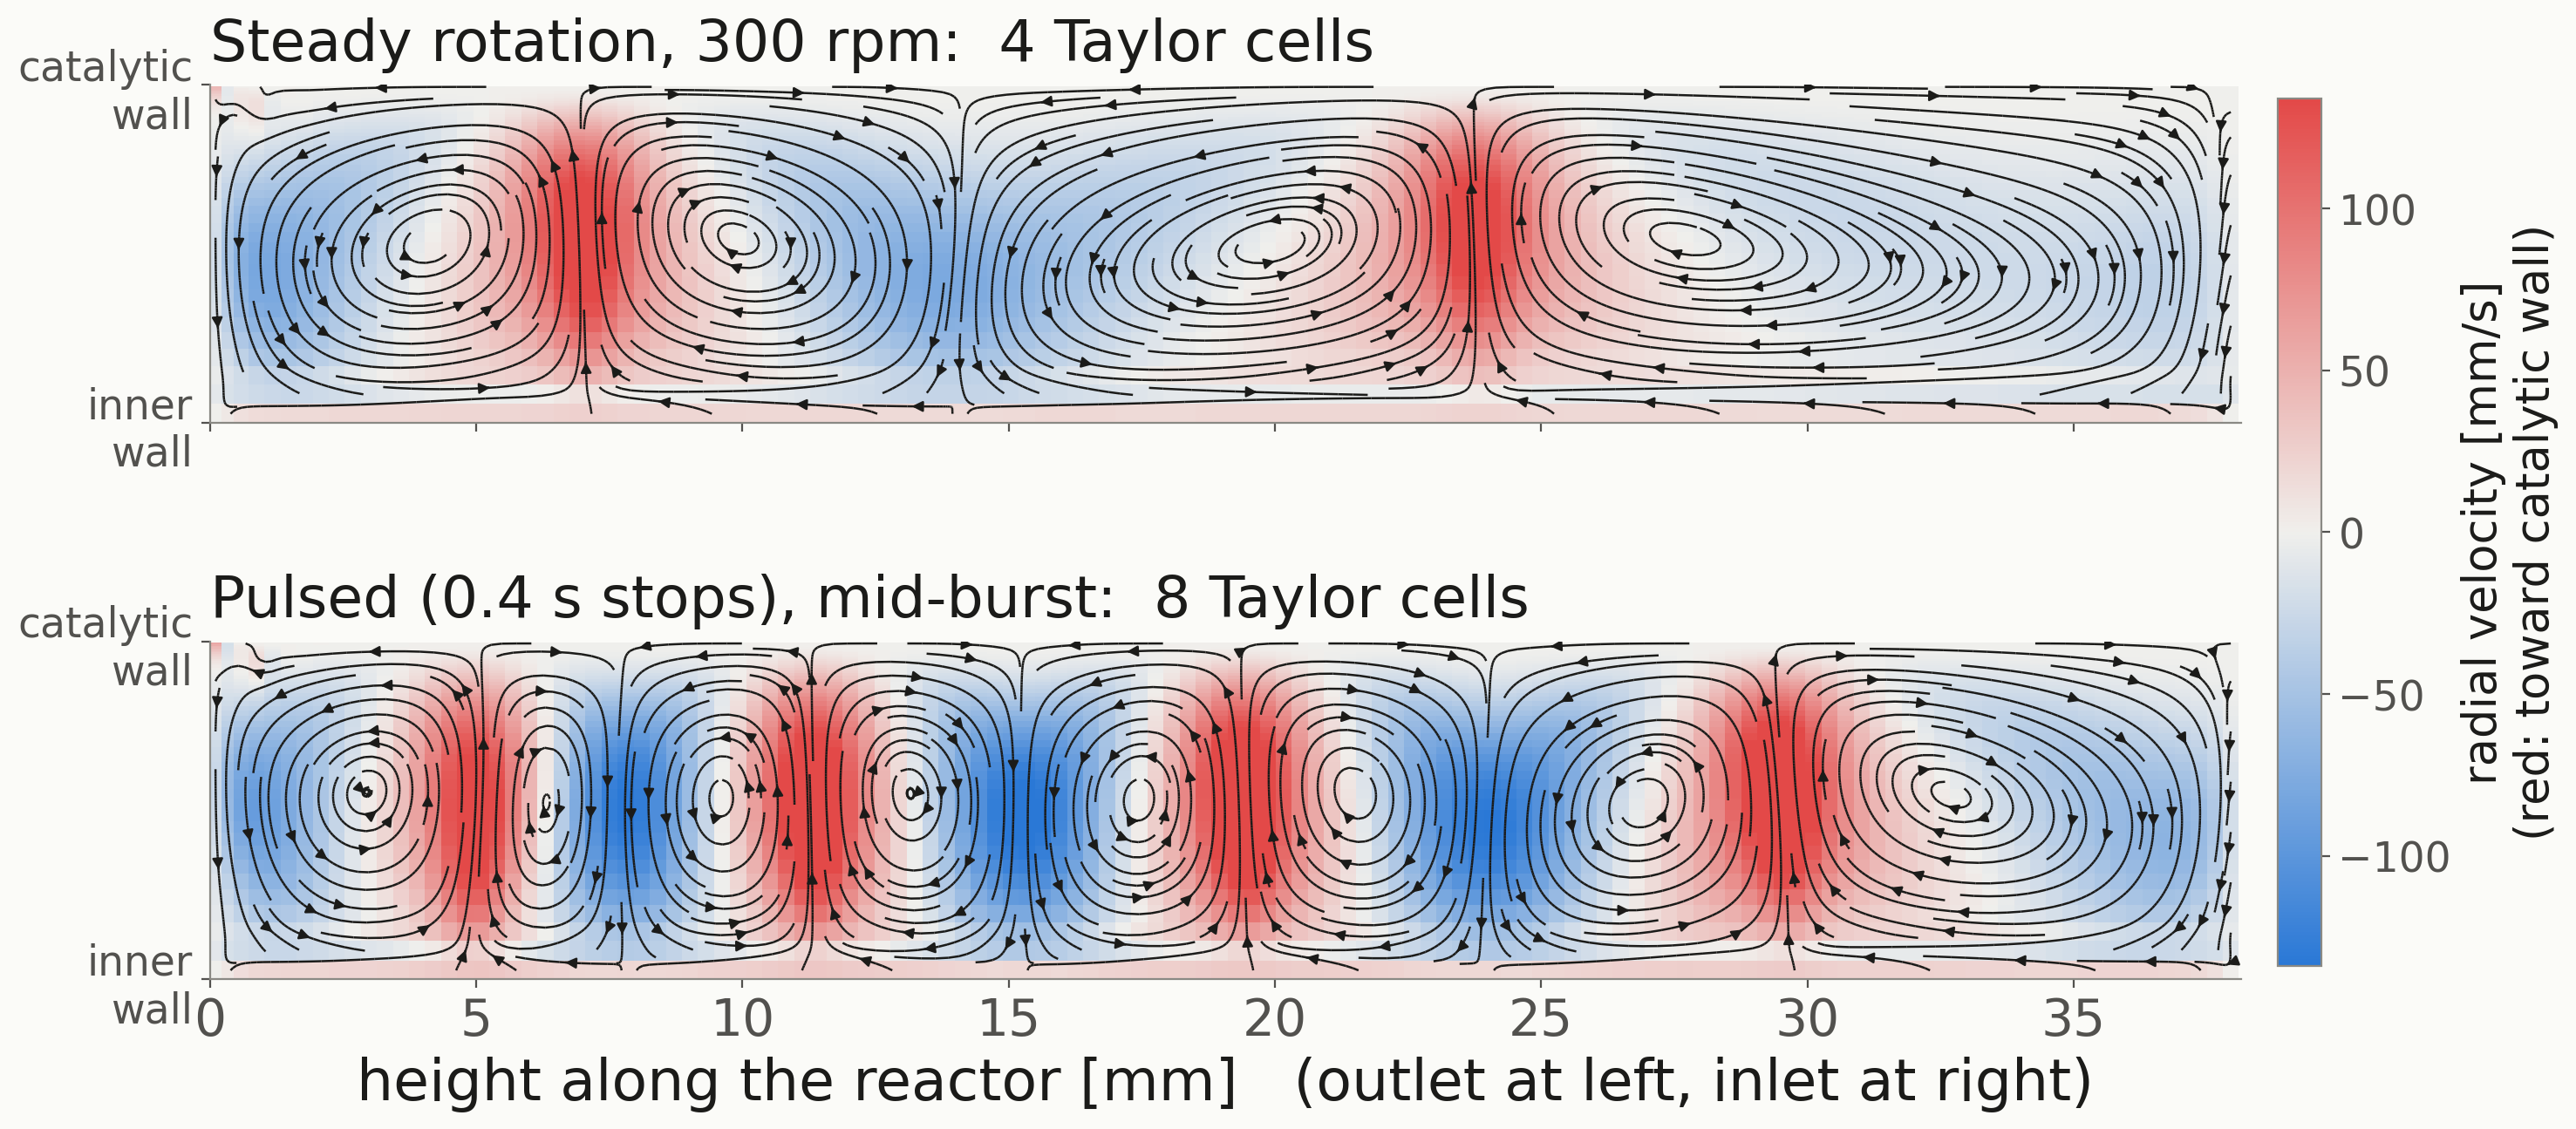
\includegraphics[width=148mm,height=30mm,keepaspectratio]{s_cells_snapshot}};
    \node[anchor=south west, inner sep=0pt, text=navy, font=\bfseries] at ([xshift=6mm,yshift=11.5mm]current page.south west)
      {Isaiah N.\ Bascom$^{1}$, \ Min Wang$^{1}$, \ Yuhe Wang$^{2}$};
    \node[anchor=south west, inner sep=0pt, text=ink, font=\scriptsize, align=left] at ([xshift=6mm,yshift=4mm]current page.south west)
      {$^{1}$Department of Mathematics, University of Houston, Houston, Texas\\
       $^{2}$Institute for Scientific Computation, Texas A\&M University, College Station, Texas};
  \end{tikzpicture}
\end{frame}
\note{[0:30] Hi, I'm Isaiah Bascom. I work on Taylor--Couette reactors: a liquid fills the gap between two cylinders, the inner one spins, and a catalyst coats the outer wall. Today's story has two parts. First, a reinforcement-learning agent found a surprisingly simple way to run this reactor better: brief full stops. Second, we found out why it works. The picture is the punchline: steady rotation gives four vortex cells, and pulsed rotation gives eight.}

% ============================================================================
\begin{frame}{The Taylor--Couette reactor}
  \begin{columns}[c]
    \begin{column}{0.60\textwidth}
      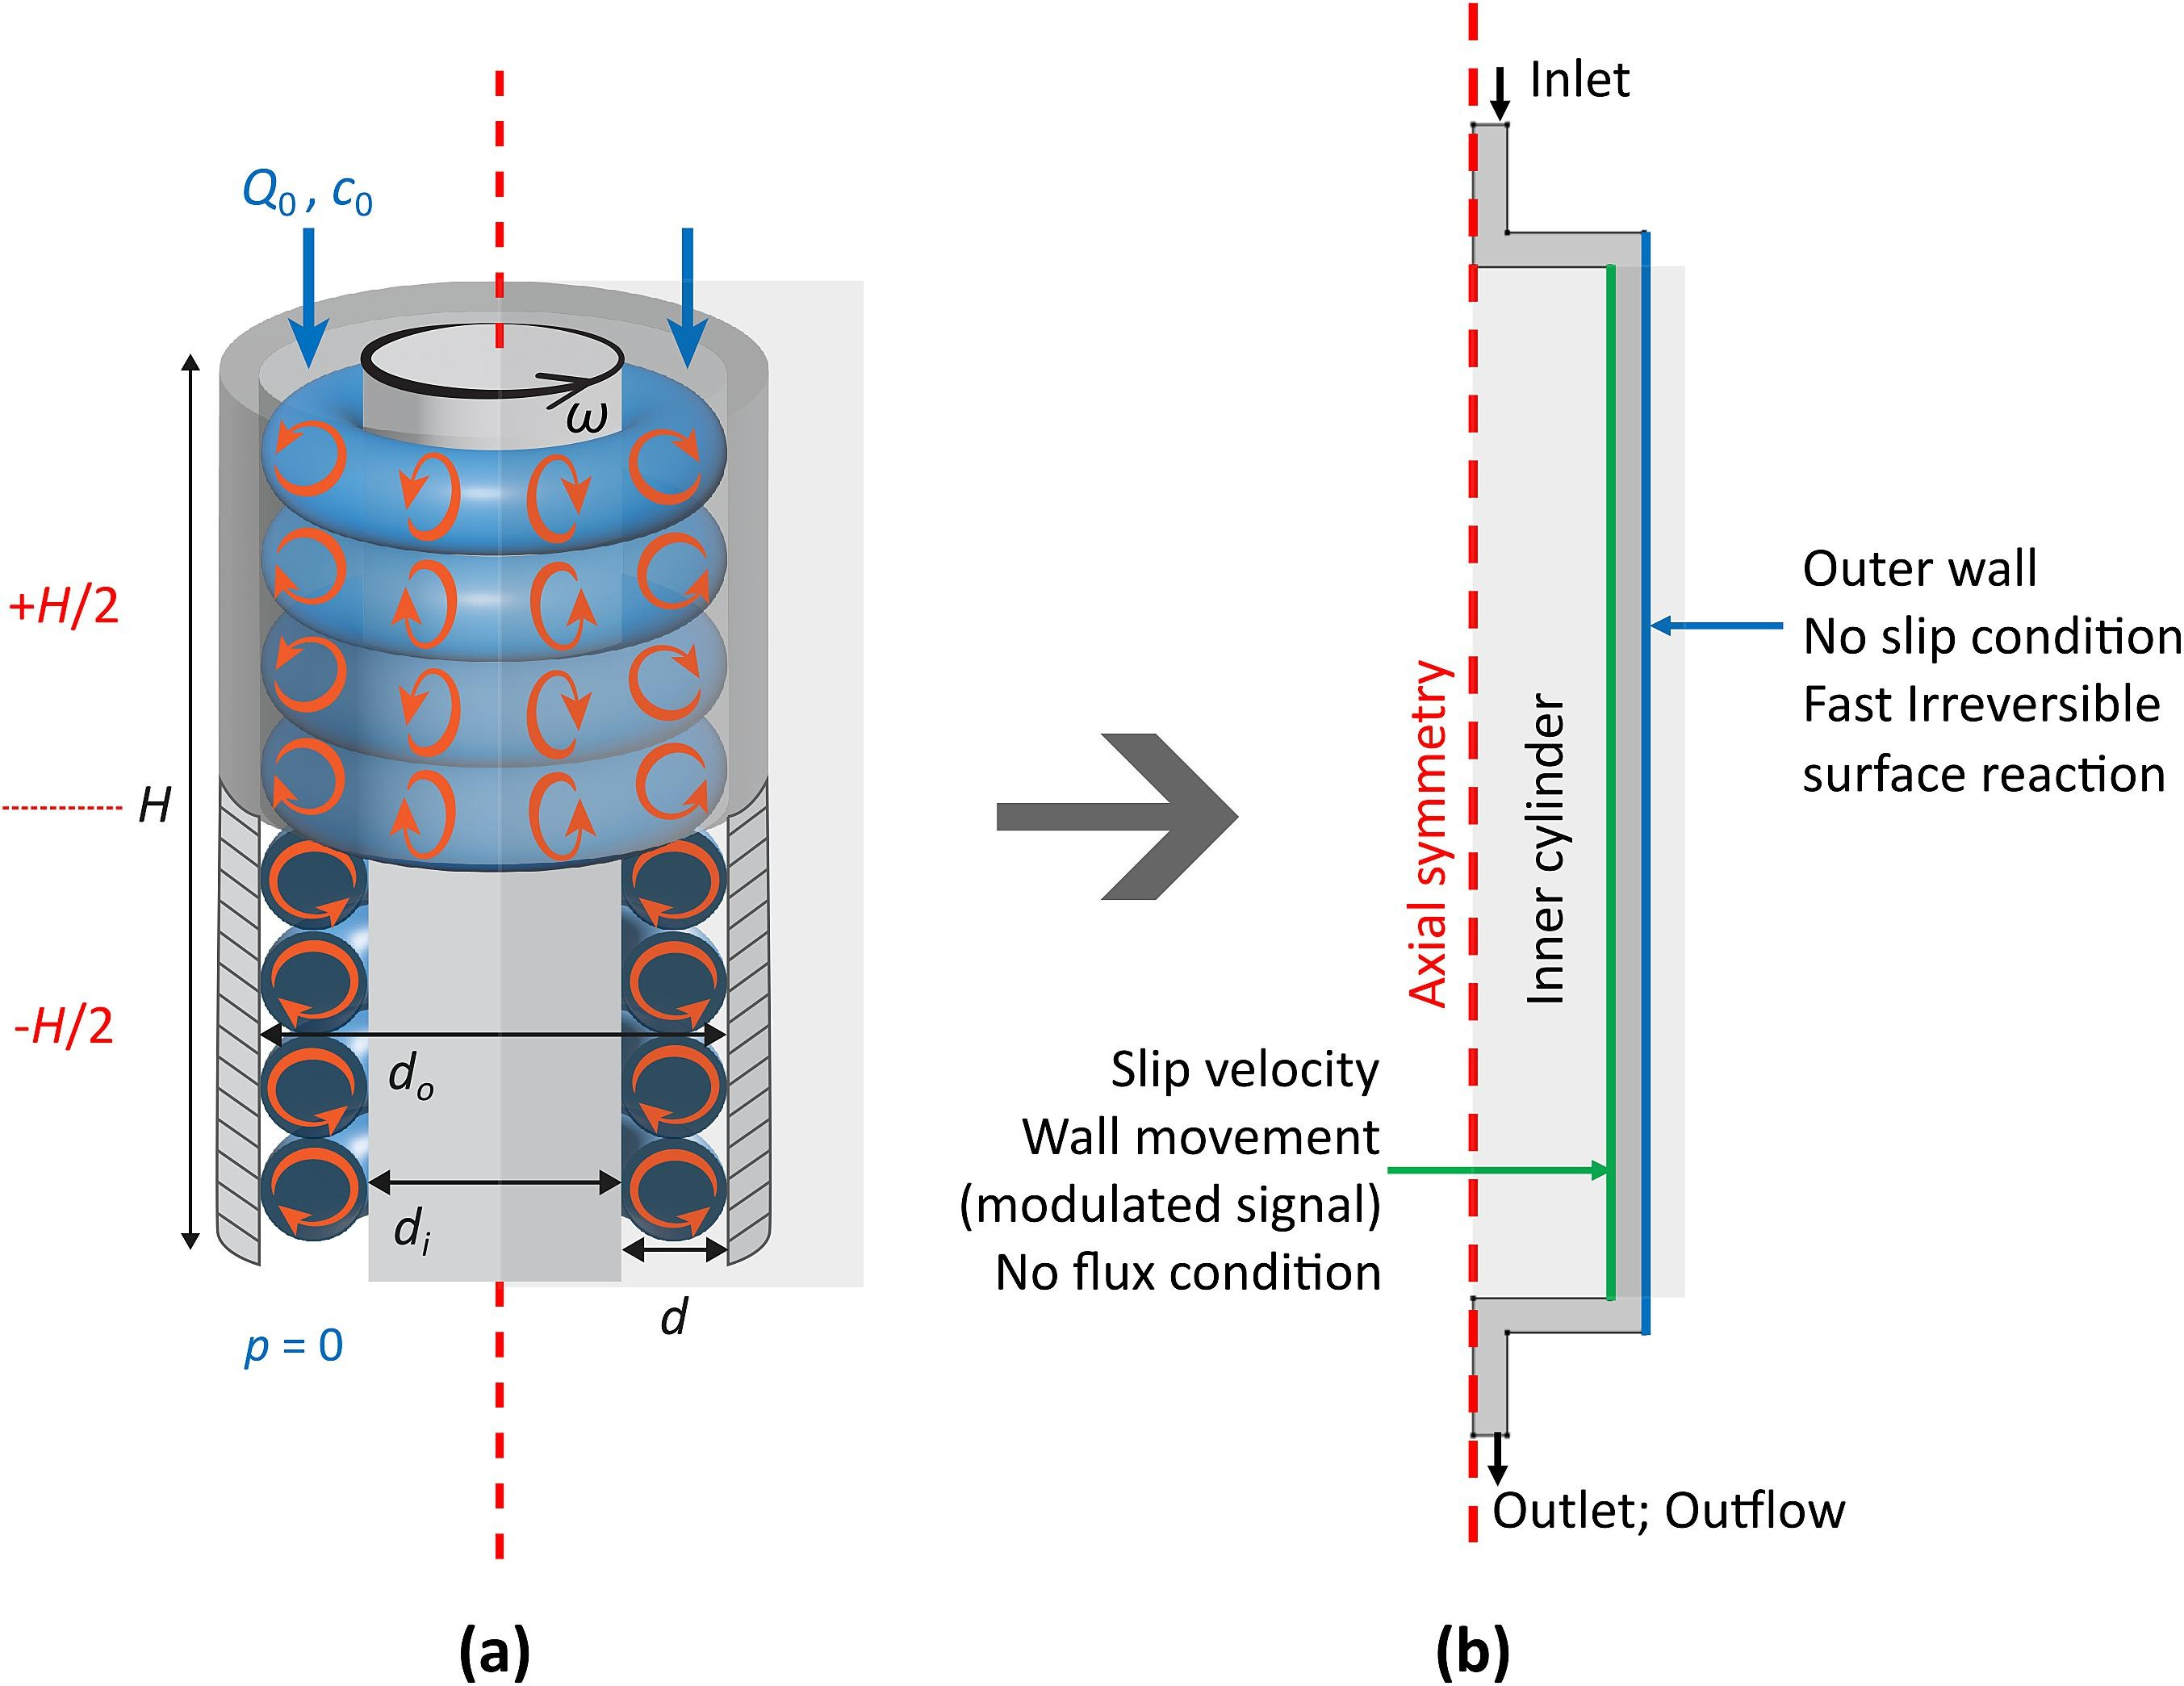
\includegraphics[width=\linewidth,height=0.78\textheight,keepaspectratio]{lg-reactor}\par
      {\tiny\color{ink}Figure: L\'opez-Guajardo et al., \emph{Chem.\ Eng.\ J.} 489 (2024) 151174, Fig.~2.}
    \end{column}
    \begin{column}{0.36\textwidth}
      {\small
      \begin{tabular*}{\linewidth}{@{}l@{\extracolsep{\fill}}r@{}}
        \toprule
        Gap $d$ & 6.35 mm \\
        $d_i$ / $d_o$ & 50.8 / 63.5 mm \\
        Height $H$ & 190.5 mm \\
        $\Gamma = H/d$ & 30 \\
        Feed $Q_0$ & 100 mL/min \\ \bottomrule
      \end{tabular*}}\par\bigskip
      Inner cylinder spins; catalyst on the outer wall.
    \end{column}
  \end{columns}
\end{frame}
\note{[0:45] First, the general setup. A Taylor--Couette reactor is liquid in the gap between two cylinders. The inner one spins, which sets up the stacked ring vortices you see on the left, the Taylor vortices. Feed enters at the top and leaves at the bottom, and the outer wall is coated with catalyst, so the reaction happens only there. The gap is about six millimetres, the reactor is about nineteen centimetres tall, an aspect ratio of thirty. Because the flow is symmetric around the axis, we can simulate just a two-dimensional slice, shown on the right; that's the standard reduction, and it's what makes reinforcement learning on this problem affordable.}

% ============================================================================
\begin{frame}{The reaction happens only at the wall}
  \begin{columns}[c]
    \begin{column}{0.52\textwidth}
      Taylor vortices carry reactant to the catalytic wall.\par\bigskip
      \begin{block}{Problem}
        Choose $\omega(t)$ for the most conversion per unit power.
      \end{block}
    \end{column}
    \begin{column}{0.46\textwidth}
      \centering
      % 2D axisymmetric domain (cf. Lopez-Guajardo et al. Fig. 2b): the fluid gap is the
      % real CFD field under the learned RL policy; everything else is drawn.
      \begin{tikzpicture}[x=1mm, y=1mm, every node/.style={font=\scriptsize}]
        \def\H{46}            % drawn height of the gap [mm]; width = H/6 (true 6.35:38.1)
        \def\W{7.67}
        \def\xg{14}           % left edge of the fluid gap
        % axis of symmetry
        \draw[uhred, dashed, line width=0.8pt] (0,-3) -- (0,\H+4);
        \node[rotate=90, text=uhred, font=\tiny] at (-2.2,\H/2) {axis of symmetry};
        % inner cylinder (schematic, not to scale in r)
        \fill[black!25] (3,0) rectangle (\xg,\H);
        \node[rotate=90, align=center, font=\tiny] at (8.5,\H/2) {inner cylinder, $\omega(t)$};
        % fluid gap: real field
        \node[anchor=south west, inner sep=0] at (\xg,0) {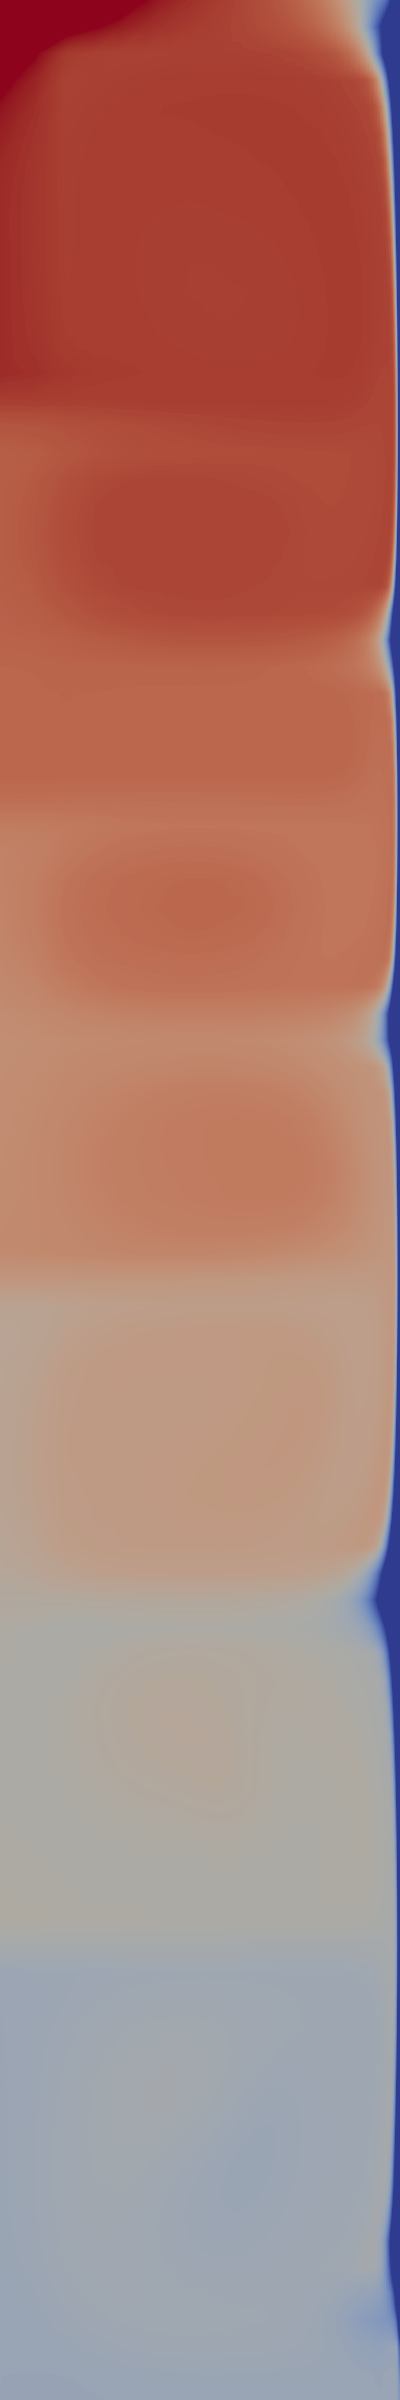
\includegraphics[width=\W mm,height=\H mm]{rl_flow_2d_conc_crop}};
        % bottom wall and catalytic outer wall (outer wall stops above the side outlet)
        \draw[black!60, line width=1.2pt] (\xg,0) -- (\xg+\W,0);
        \definecolor{wallblue}{HTML}{3B4CC0}   % bottom of the concentration scale: c = 0
        \draw[wallblue, line width=1.6pt] (\xg+\W+0.6,1.4) -- (\xg+\W+0.6,\H);
        % inlet at the top of the gap
        \draw[-{Latex[length=2mm]}, navy, line width=1pt] (\xg+\W/2,\H+6) -- (\xg+\W/2,\H+0.6);
        \node[anchor=south] at (\xg+\W/2,\H+6) {inlet};
        % side outlet: the bottom 0.42 mm of the outer wall
        \draw[-{Latex[length=2mm]}, navy, line width=1pt] (\xg+\W+0.2,0.7) -- (\xg+\W+7,0.7);
        \node[anchor=west, align=left] at (\xg+\W+7.3,0.9) {\textbf{side outlet}};
        % labels
        \node[anchor=west, align=left, text=wallblue, font=\scriptsize\bfseries] at (\xg+\W+2.2,\H*0.62)
          {catalytic wall\\[-1pt]{\normalfont\tiny $c = 0$}};
        % concentration key (ParaView "Cool to Warm", matching the render's 0.45-0.88 c/c0 range)
        \definecolor{cw0}{HTML}{3B4CC0}\definecolor{cw1}{HTML}{DDDDDD}\definecolor{cw2}{HTML}{B40426}
        \shade[bottom color=cw0, top color=cw1] (\xg+\W+3,\H*0.22) rectangle (\xg+\W+5,\H*0.32);
        \shade[bottom color=cw1, top color=cw2] (\xg+\W+3,\H*0.32) rectangle (\xg+\W+5,\H*0.42);
        \node[anchor=west, font=\tiny, text=ink] at (\xg+\W+5.4,\H*0.42) {reactant};
        \node[anchor=west, font=\tiny, text=ink] at (\xg+\W+5.4,\H*0.22) {product};
      \end{tikzpicture}\par\smallskip
    \end{column}
  \end{columns}
\end{frame}
\note{[0:45] The reaction only happens on the catalytic outer wall, so everything depends on how fast reactant gets carried from the bulk to that wall. The Taylor vortices in the gap do that carrying. Changing the rotation over time can beat spinning at a constant speed. The picture is the 2D plane our simulation actually solves on, with the real flow under the learned policy: the spinning inner cylinder on the left, the liquid gap coloured by concentration, and the catalytic wall on the right. Red is fresh reactant; blue is where it has been converted to product. You can see the thin blue layer along the catalytic wall, and the vortices peeling that converted liquid off the wall and bringing fresh reactant in. Fluid enters at the top and leaves through a side outlet at the bottom of the outer wall. So this is a control problem governed by PDEs: choose the speed as a function of time to get the most reactant converted for the power spent. What is the optimal control, and why does it work?}

% ============================================================================
\begin{frame}{Non-turbulent flow and scalar transport}
  \begin{columns}[T]
    \begin{column}{0.56\textwidth}
      \begin{block}{Equations}
        \setlength{\abovedisplayskip}{5pt}\setlength{\belowdisplayskip}{5pt}%
        Laminar incompressible flow with constant viscosity and no turbulence model
        \begin{gather*}
          \nabla\cdot\mathbf{u} = 0\\
          \frac{\partial\mathbf{u}}{\partial t} + (\mathbf{u}\cdot\nabla)\mathbf{u} = -\nabla p + \nu\,\nabla^2\mathbf{u}
        \end{gather*}
        Scalar-transport equation
        \[ \frac{\partial c}{\partial t} + \mathbf{u}\cdot\nabla c = D\,\nabla^2 c \]
      \end{block}
    \end{column}
    \begin{column}{0.40\textwidth}
      \begin{block}{Numerics}
        Finite volume (OpenFOAM), 2D axisymmetric; 3330 cells graded to 25\,$\mu$m at the catalytic wall\par\smallskip
        Inner wall: $\omega(t)$\\ Catalytic wall: $c = 0$\\ Inlet: $c = c_0$\par\smallskip
        $\mathrm{Re}\approx 470$, \ $\mathrm{Sc}=1075$
      \end{block}
    \end{column}
  \end{columns}
  \medskip
  \begin{beamercolorbox}[wd=\textwidth,sep=8pt,rounded=true]{frametitle}
    \begin{tabular}{@{}l@{\ }l@{}}
      \textbf{Objective:} & $\max\; X - P/P_{\max}$ \quad s.t. \ $\overline{\omega} = 300$ rpm\\[2pt]
      & {\small $X = 1 - \bar c_{\mathrm{out}}/c_0$ (conversion), \ $P$ = motor power}
    \end{tabular}
  \end{beamercolorbox}
\end{frame}
\note{[0:45] Incompressible Navier--Stokes for the flow, solved axisymmetrically but keeping the swirl component, and an advection--diffusion equation for the reactant. The inner wall turns at a prescribed omega of t. On the catalytic wall the concentration is zero, so the reaction rate is set entirely by how fast reactant diffuses in. Finite-volume discretization in OpenFOAM, with the mesh graded to 25 microns at the wall because the concentration layer there is thin: the Schmidt number is about a thousand. The objective rewards conversion and penalizes motor power. We also fix the mean speed at 300 rpm, which in practice fixes the power, so every candidate is compared at the same power and the question becomes how much conversion each one gets for it.}

% ============================================================================
\begin{frame}{Three ways to search an expensive simulator}
  \begin{columns}[T]
    \begin{column}{0.32\textwidth}
      \begin{block}{\begin{tabular}[t]{@{}l@{\ }l@{}}Discover: & reinforcement\\ & learning\end{tabular}}
        TD3 actor--critic. State: conversion and time. Action: burst and stop lengths. Reward: conversion. No physics given.
      \end{block}
    \end{column}
    \begin{column}{0.32\textwidth}
      \begin{block}{\begin{tabular}[t]{@{}l@{\ }l@{}}Check: & Bayesian\\ & optimization\end{tabular}}
        Gaussian-process surrogate (Mat\'ern-5/2) with expected improvement; 220 CFD runs over fixed waveforms. Replicate noise $\sigma\approx 0.002$.
      \end{block}
    \end{column}
    \begin{column}{0.32\textwidth}
      \begin{block}{\begin{tabular}[t]{@{}l@{\ }l@{}}Explain: & designed\\ & experiments\end{tabular}}
        Pre-registered hypotheses, 62 targeted runs, flow diagnostics logged every 0.02\,s.
      \end{block}
    \end{column}
  \end{columns}
  \bigskip
  \takeaway{Each 130\,s simulation costs about 3--4 CPU-hours, so every method has to be sample-efficient.}
\end{frame}
\note{[0:45] Each simulated episode costs a few CPU-hours, so I used three complementary tools. Reinforcement learning, with TD3, an actor--critic method, to discover a strategy without being told any physics: it sees only the conversion and the time, and chooses how long to run and how long to stop. Bayesian optimization, with a Gaussian-process surrogate and expected improvement over 220 simulations, as an independent check. And designed experiments, with hypotheses written down in advance, to explain why the answer works.}

% ============================================================================
\begin{frame}{Reinforcement learning found brief full stops}
  \alert{All 5 runs: brief full stops (0.1--0.4\,s), never long idles.}\par\medskip
  \centering\includegraphics[width=\linewidth,height=0.66\textheight,keepaspectratio]{fig4_learned_waveform}
\end{frame}
\note{[0:45] Here's what the reinforcement-learning agent did, with the average held at 300 rpm. What it learned, in all five independent training runs, is the same kind of policy: run a little above 300 rpm for a few seconds, then stop completely for a fraction of a second, mostly a tenth to four tenths of a second, and repeat. None of them learned long idles. That was not the answer I expected, and it's the opposite of the published recipe.}

% ============================================================================
\begin{frame}{The opposite of the published recipe}
  \begin{columns}[c]
    \begin{column}{0.60\textwidth}
      \includegraphics[width=\linewidth,height=0.74\textheight,keepaspectratio]{fig5_recipe_contrast}
    \end{column}
    \begin{column}{0.38\textwidth}
      \begin{block}{Bayesian optimization}Stop 0.5\,s every 5\,s\end{block}
      \begin{block}{RL}Within 0.01--0.02 of it\end{block}
      \begin{block}{Published recipe}Best in their model, not ours\end{block}
    \end{column}
  \end{columns}
\end{frame}
\note{[0:45] On top, the published recipe: burst to 2500 rpm for six seconds, then sit still for twenty-four. Below, what the agent found. The Bayesian-optimization search over 220 fixed waveforms found the same thing: stop for about half a second every five seconds. The learned policies stop a little shorter, mostly 0.1 to 0.4 seconds, and come within one to two hundredths of conversion of that best fixed waveform, so RL matched the search rather than beating it. Later we'll see why the shorter stops cost a little: they mostly land in the six-cell state rather than eight. The published recipe was the best policy in their model, but in ours it loses even to steady rotation. One note: my submitted abstract describes long low-speed periods with short bursts. The result turned out to be the opposite, brief full stops at high duty, and this slide is the correction.}

% ============================================================================
\begin{frame}{It transfers to a reactor five times taller}
  \begin{columns}[c]
    \begin{column}{0.52\textwidth}
      \includegraphics[width=\linewidth,height=0.74\textheight,keepaspectratio]{fig1_conversion_vs_power}
    \end{column}
    \begin{column}{0.46\textwidth}
      {\small
      \begin{tabular*}{\linewidth}{@{}l@{\extracolsep{\fill}}r@{}}
        \toprule
        Tall reactor & Conversion \\ \midrule
        RL, no retraining & 0.90 \\
        Best fixed waveform & 0.91 \\
        Steady, same power & 0.79 \\
        Published, $1.7\times$ power & 0.76 \\ \bottomrule
      \end{tabular*}}
    \end{column}
  \end{columns}
\end{frame}
\note{[0:45] Then a generalization test: the policy trained on the short reactor, run with no retraining on a reactor five times taller. The blue line is steady rotation at different speeds. The red star is the transferred policy: 0.90 conversion at 3.7 watts, against 0.79 for steady rotation at the same power. It ties the best fixed waveform at 0.91. The grey triangle is the published recipe: 0.76 while using about 1.7 times the power. Caveat in small print: these tall-reactor runs used the original time step, so trust the ranking more than the third decimal.}

% ============================================================================
\begin{frame}{Why it works: each restart builds more vortex cells}
  \centering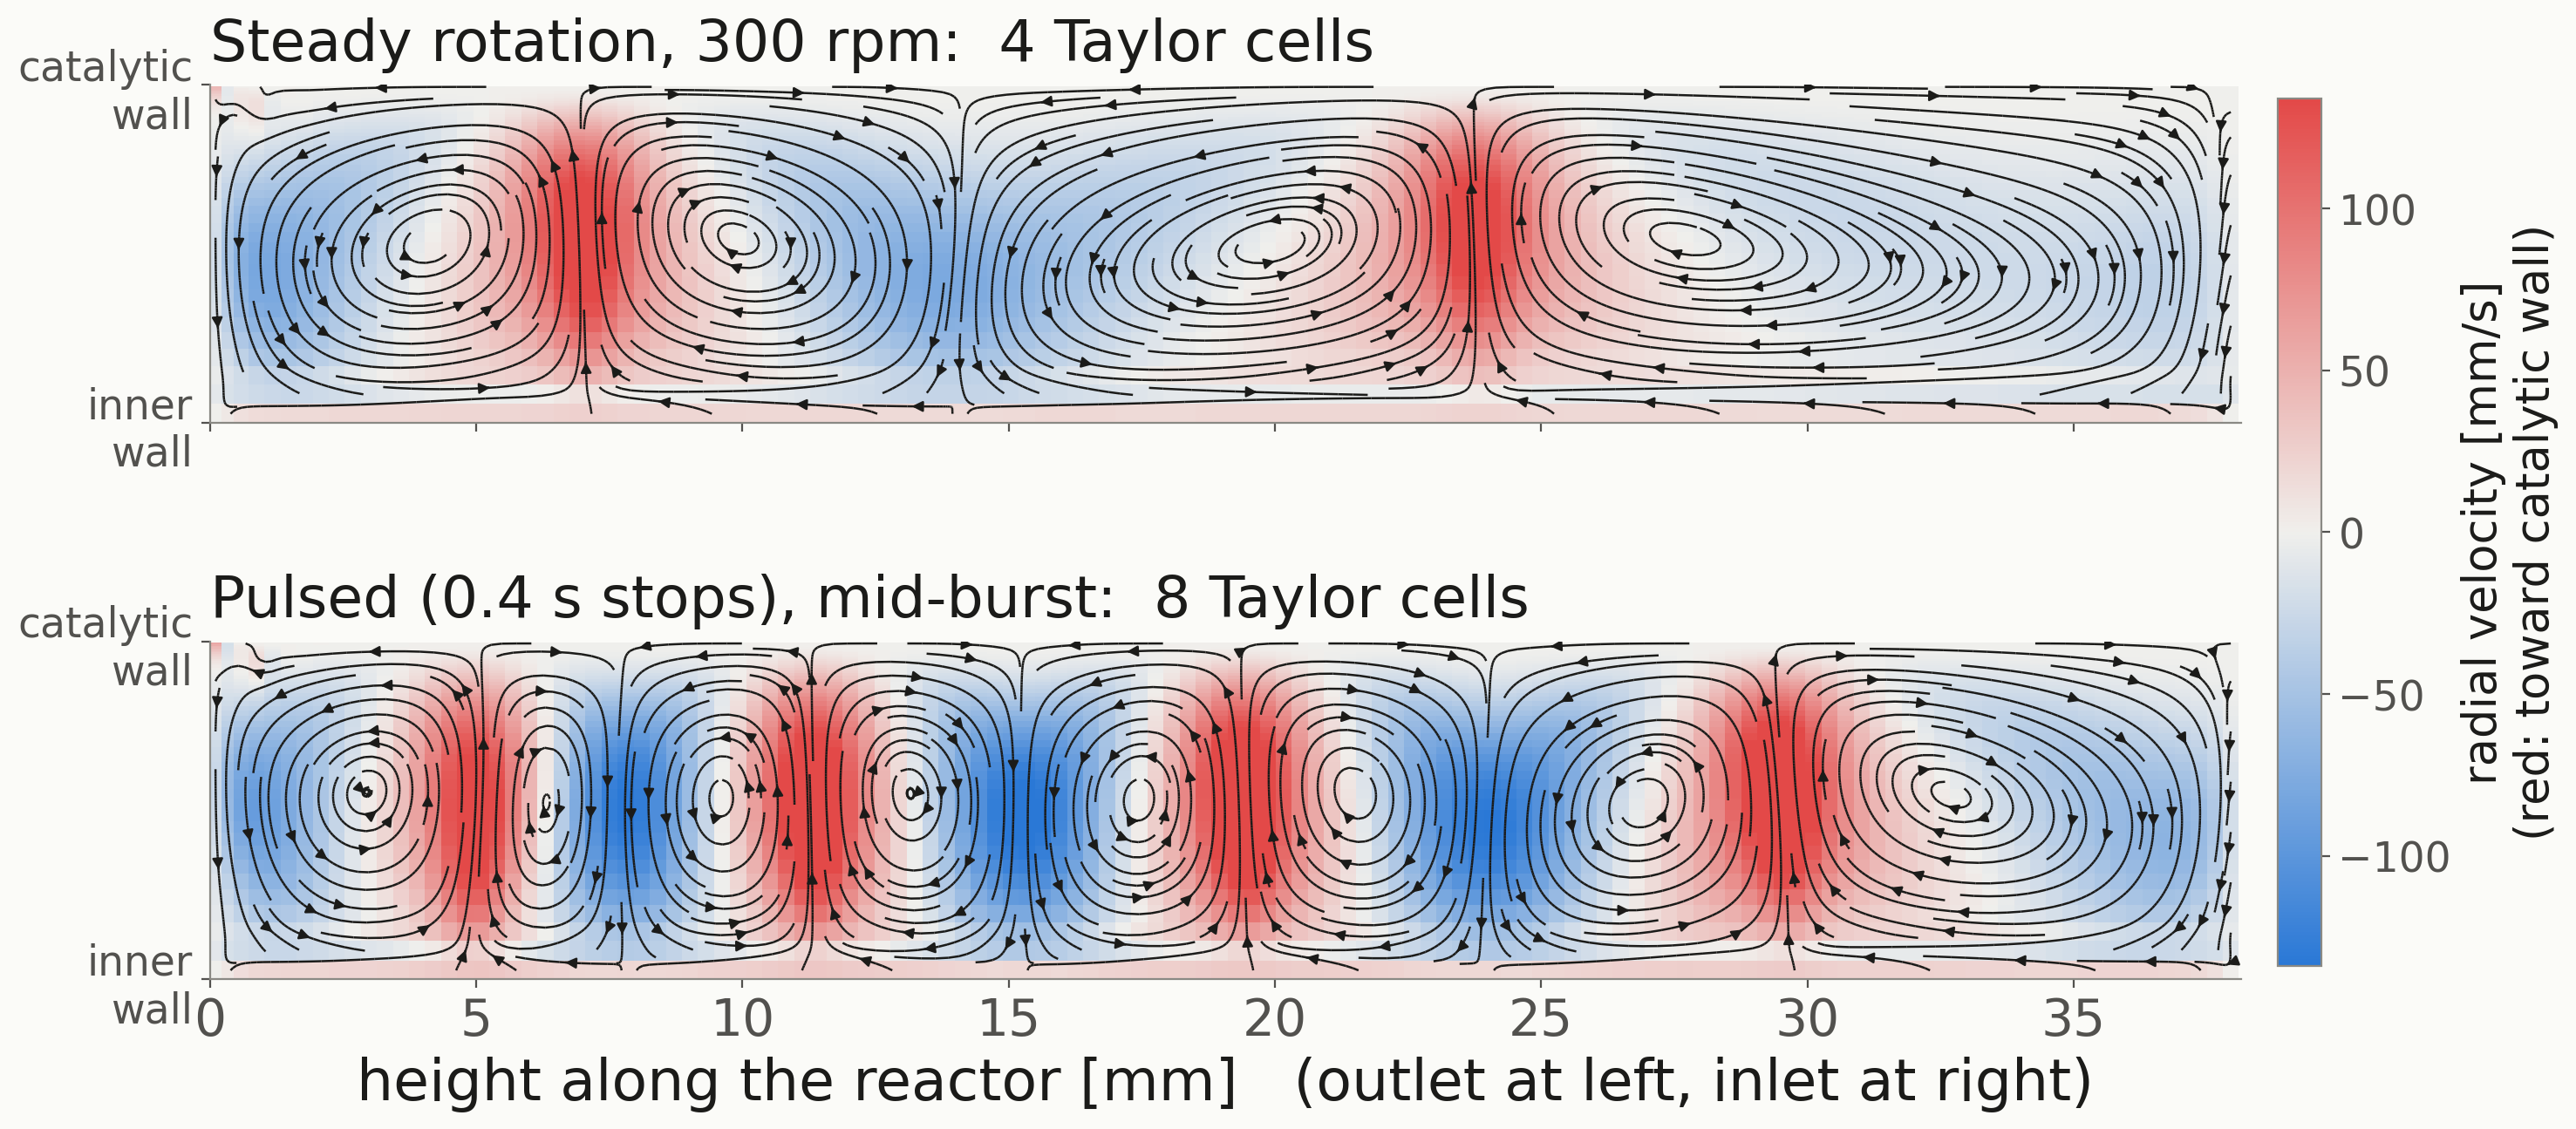
\includegraphics[width=\linewidth,height=0.86\textheight,keepaspectratio]{s_cells_snapshot}
\end{frame}
\note{[1:00] So why does a brief stop help? Both panels show the gap between the cylinders, unrolled sideways: inner wall at the bottom, catalytic wall at the top. Colour is radial velocity; red means liquid heading toward the catalytic wall. Under steady rotation there are four large vortex cells. Under pulsing, mid-burst, there are eight narrower ones. In dynamical-systems language this is multistability: at the same Reynolds number a short Taylor--Couette annulus has several stable solutions with different numbers of cells, and which one you land in depends on the initial condition; Benjamin and Mullin studied this in the early 1980s (check citation). Each brief stop brings the flow nearly to rest, and the restart from rest selects a higher axial wavenumber, eight cells instead of four. Narrower cells carry reactant to the wall faster.}

% ============================================================================
\begin{frame}{Restarts make the extra cells; steady rotation erases them}
  \begin{columns}[T]
    \begin{column}{0.49\textwidth}
      \centering{\small\textbf{Each cycle:} 8 cells, +15\% wall reaction}\par\smallskip
      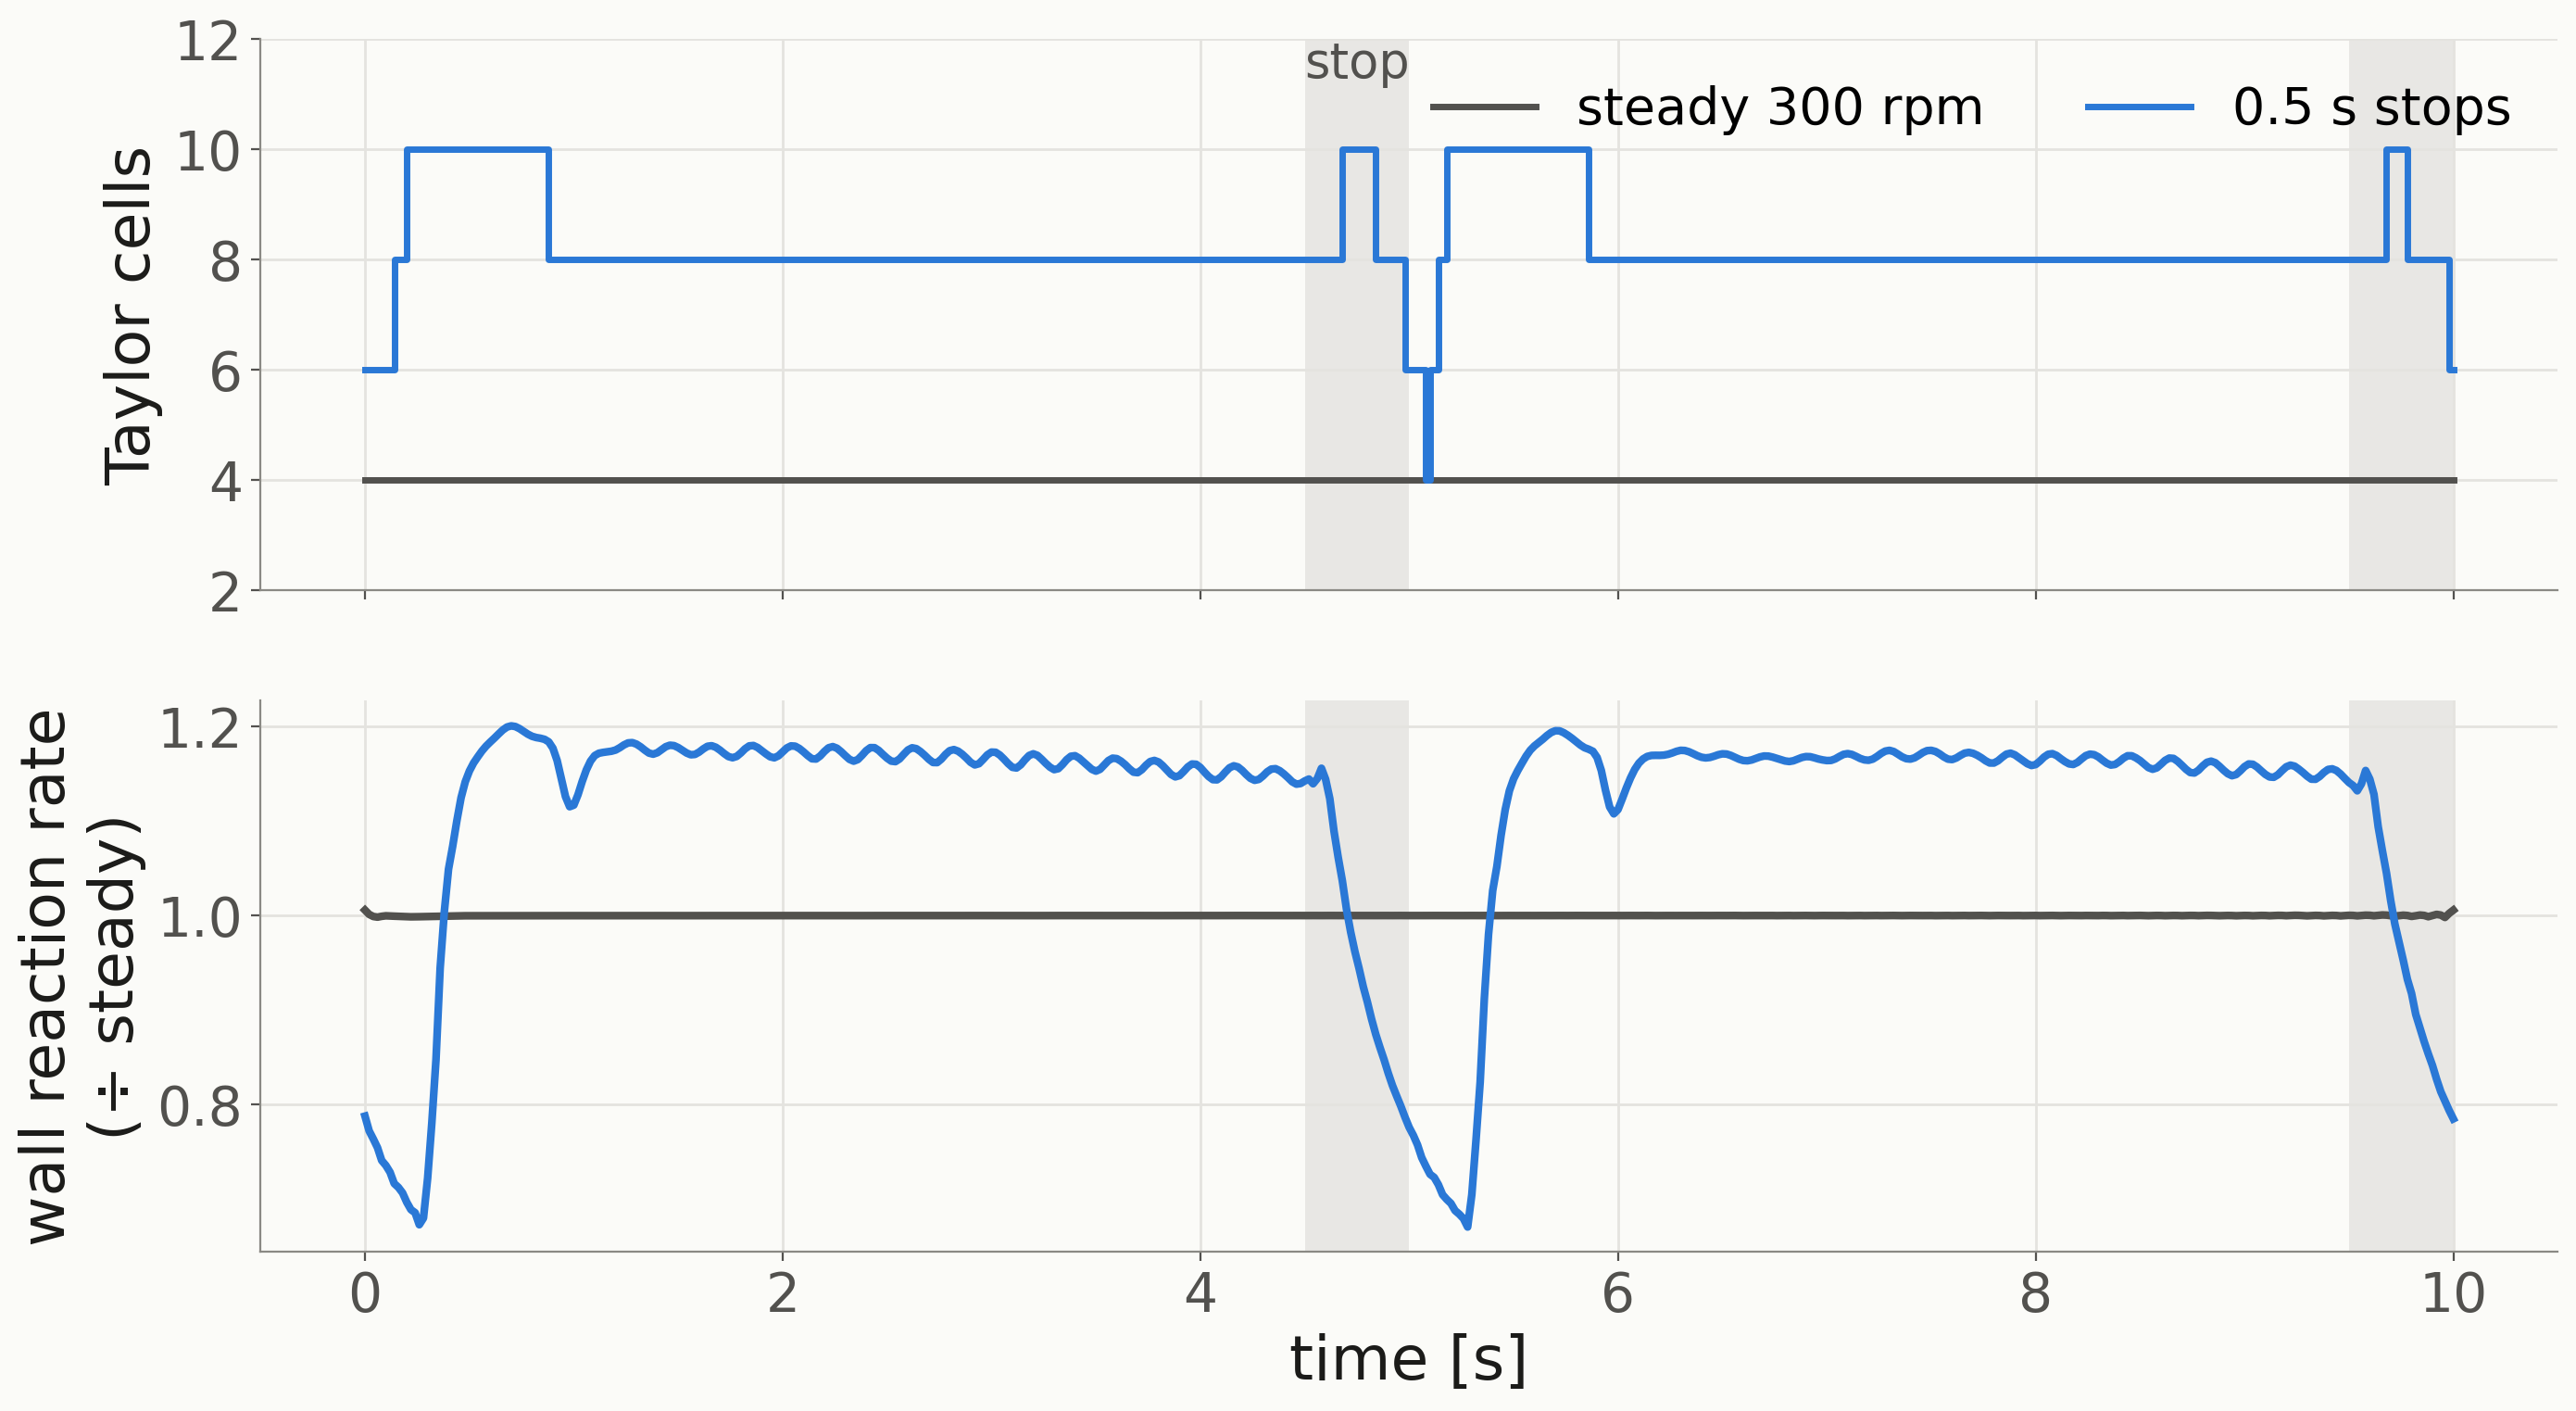
\includegraphics[width=\linewidth,height=0.56\textheight,keepaspectratio]{s_one_cycle}
    \end{column}
    \begin{column}{0.49\textwidth}
      \centering{\small\textbf{Stop pulsing:} back to 4 cells in 10--15\,s}\par\smallskip
      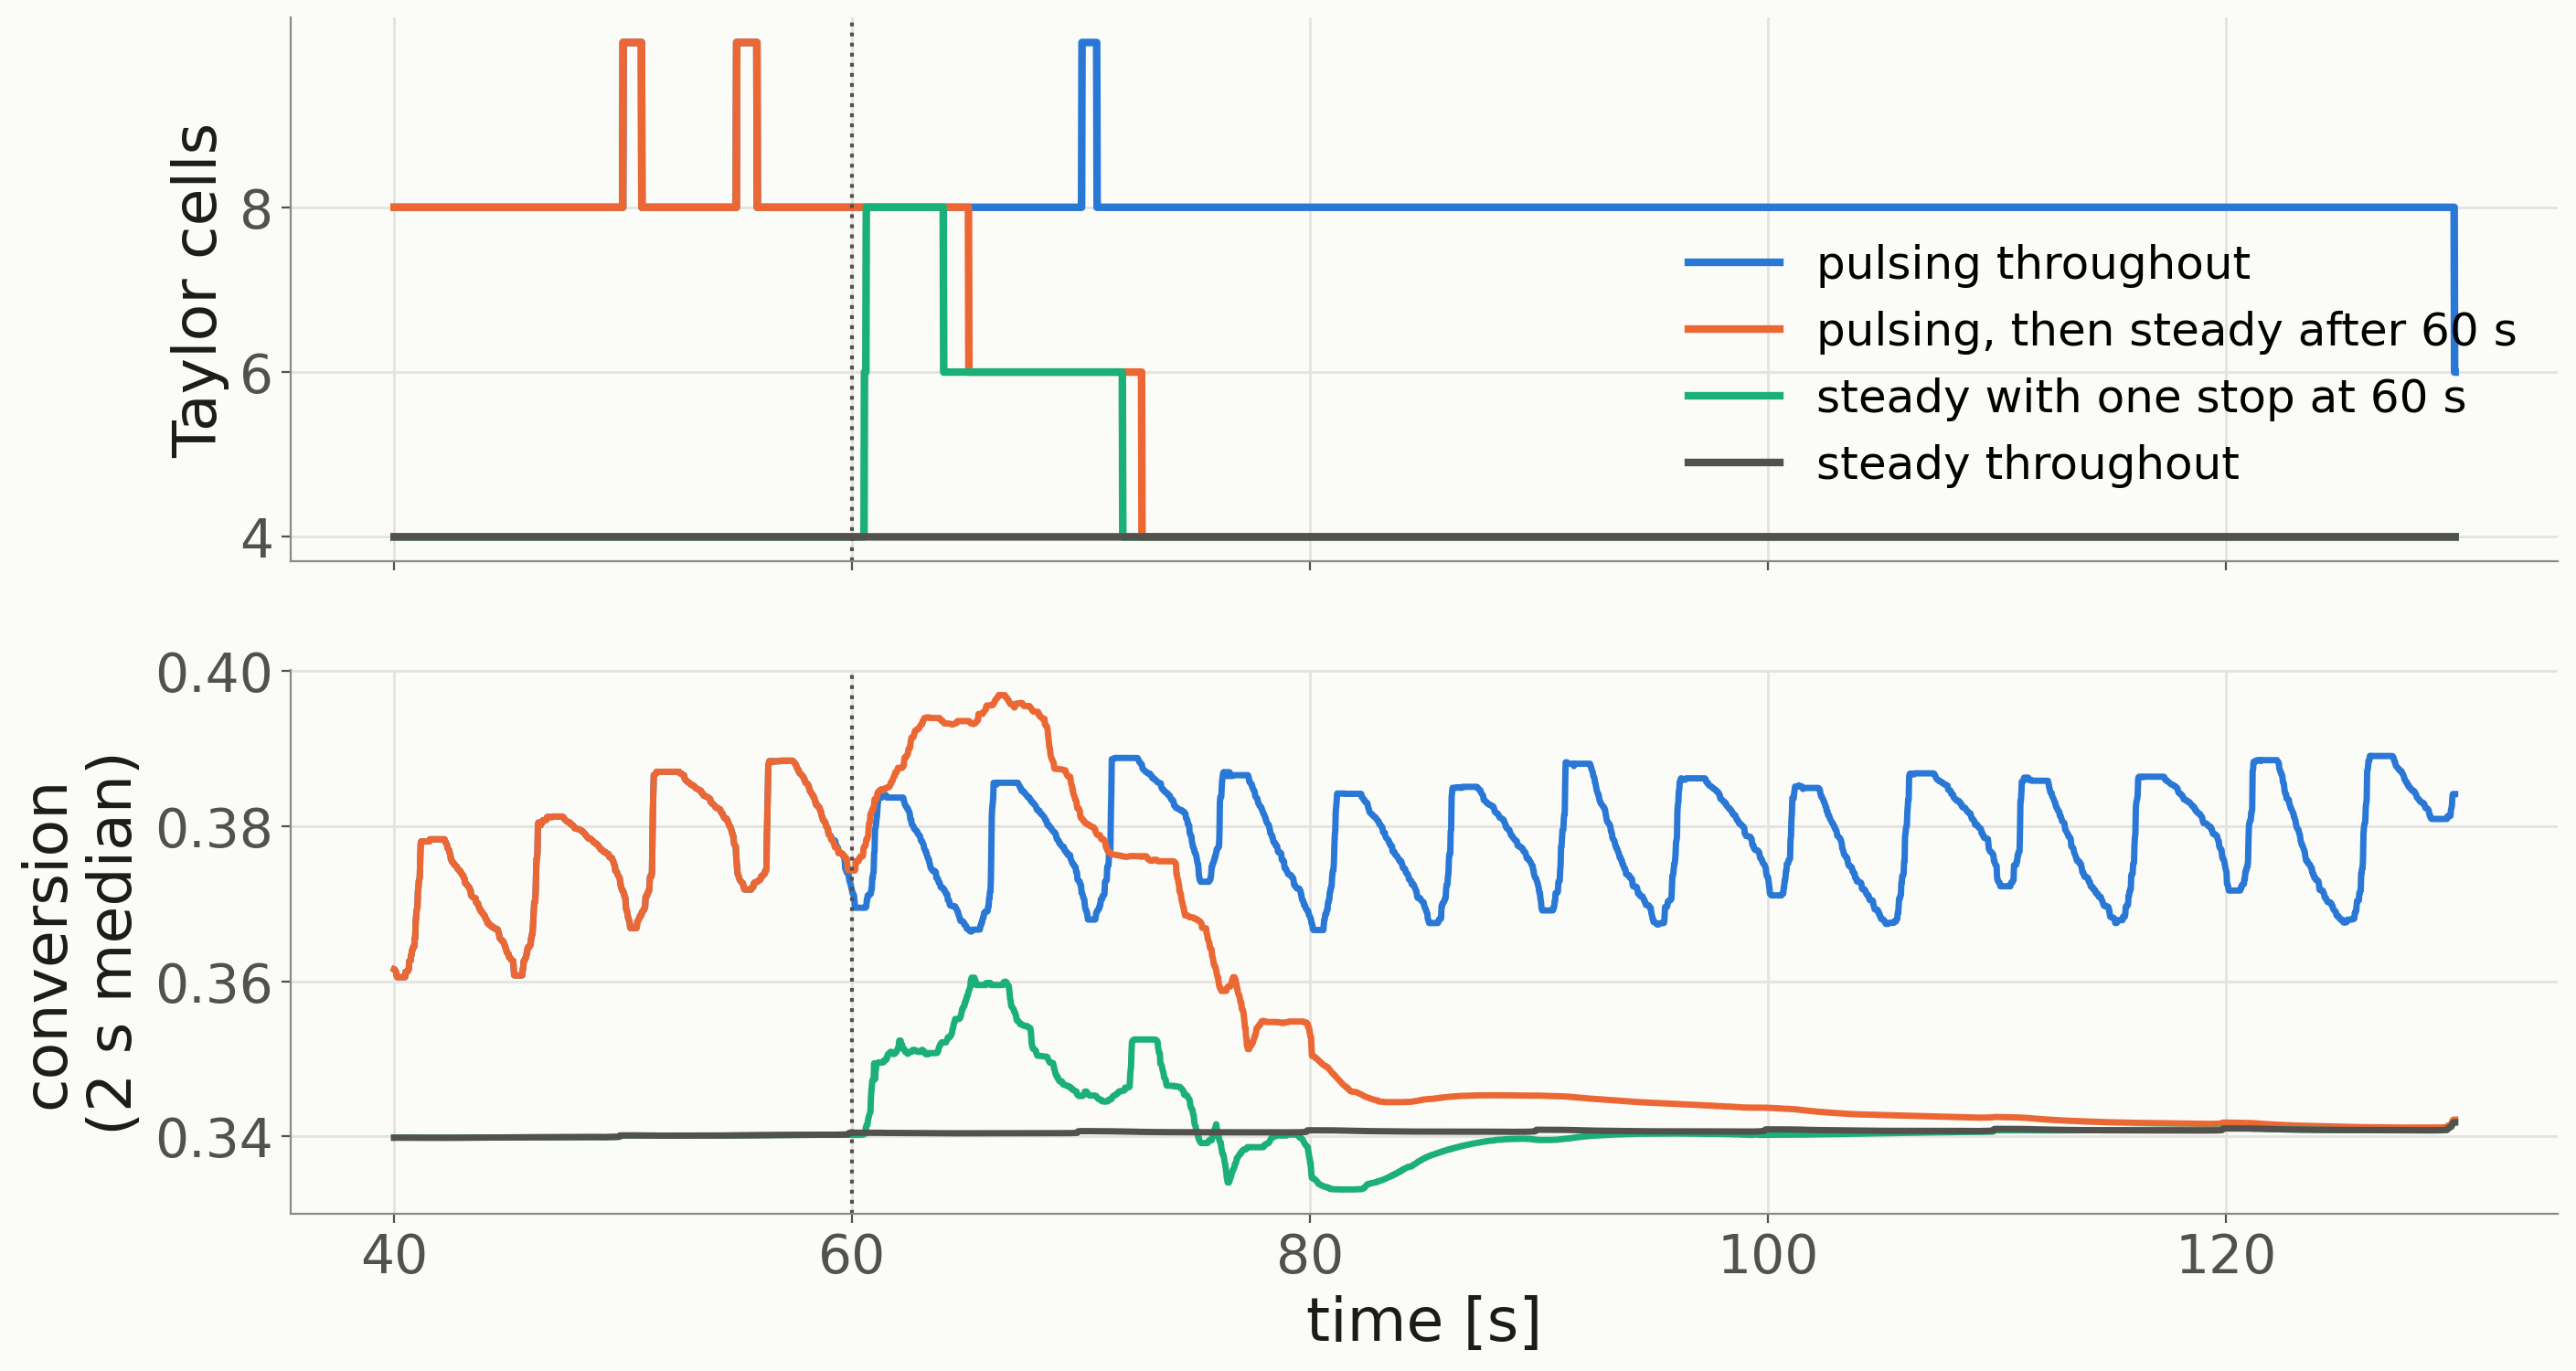
\includegraphics[width=\linewidth,height=0.56\textheight,keepaspectratio]{s_hold_kick}
    \end{column}
  \end{columns}
  \medskip
  \centering\alert{\textbf{Stops must repeat.}}
\end{frame}
\note{[1:00] Inside each cycle: after every restart the cell count jumps up and settles at eight, and the reaction rate at the wall stays about fifteen percent above steady rotation for the whole burst. It isn't a brief spike after the restart; the restart spike contributes almost nothing. On the right: if I pulse until 60 seconds and then hold steady, or do just one stop, the extra cells merge back to four within ten to fifteen seconds, and conversion drops back to the steady value. So the stops have to keep coming every few seconds, which explains why five-second cycles win and the published thirty-second cycle loses.}

% ============================================================================
\begin{frame}{It has to be a full stop}
  \begin{columns}[c]
    \begin{column}{0.68\textwidth}
      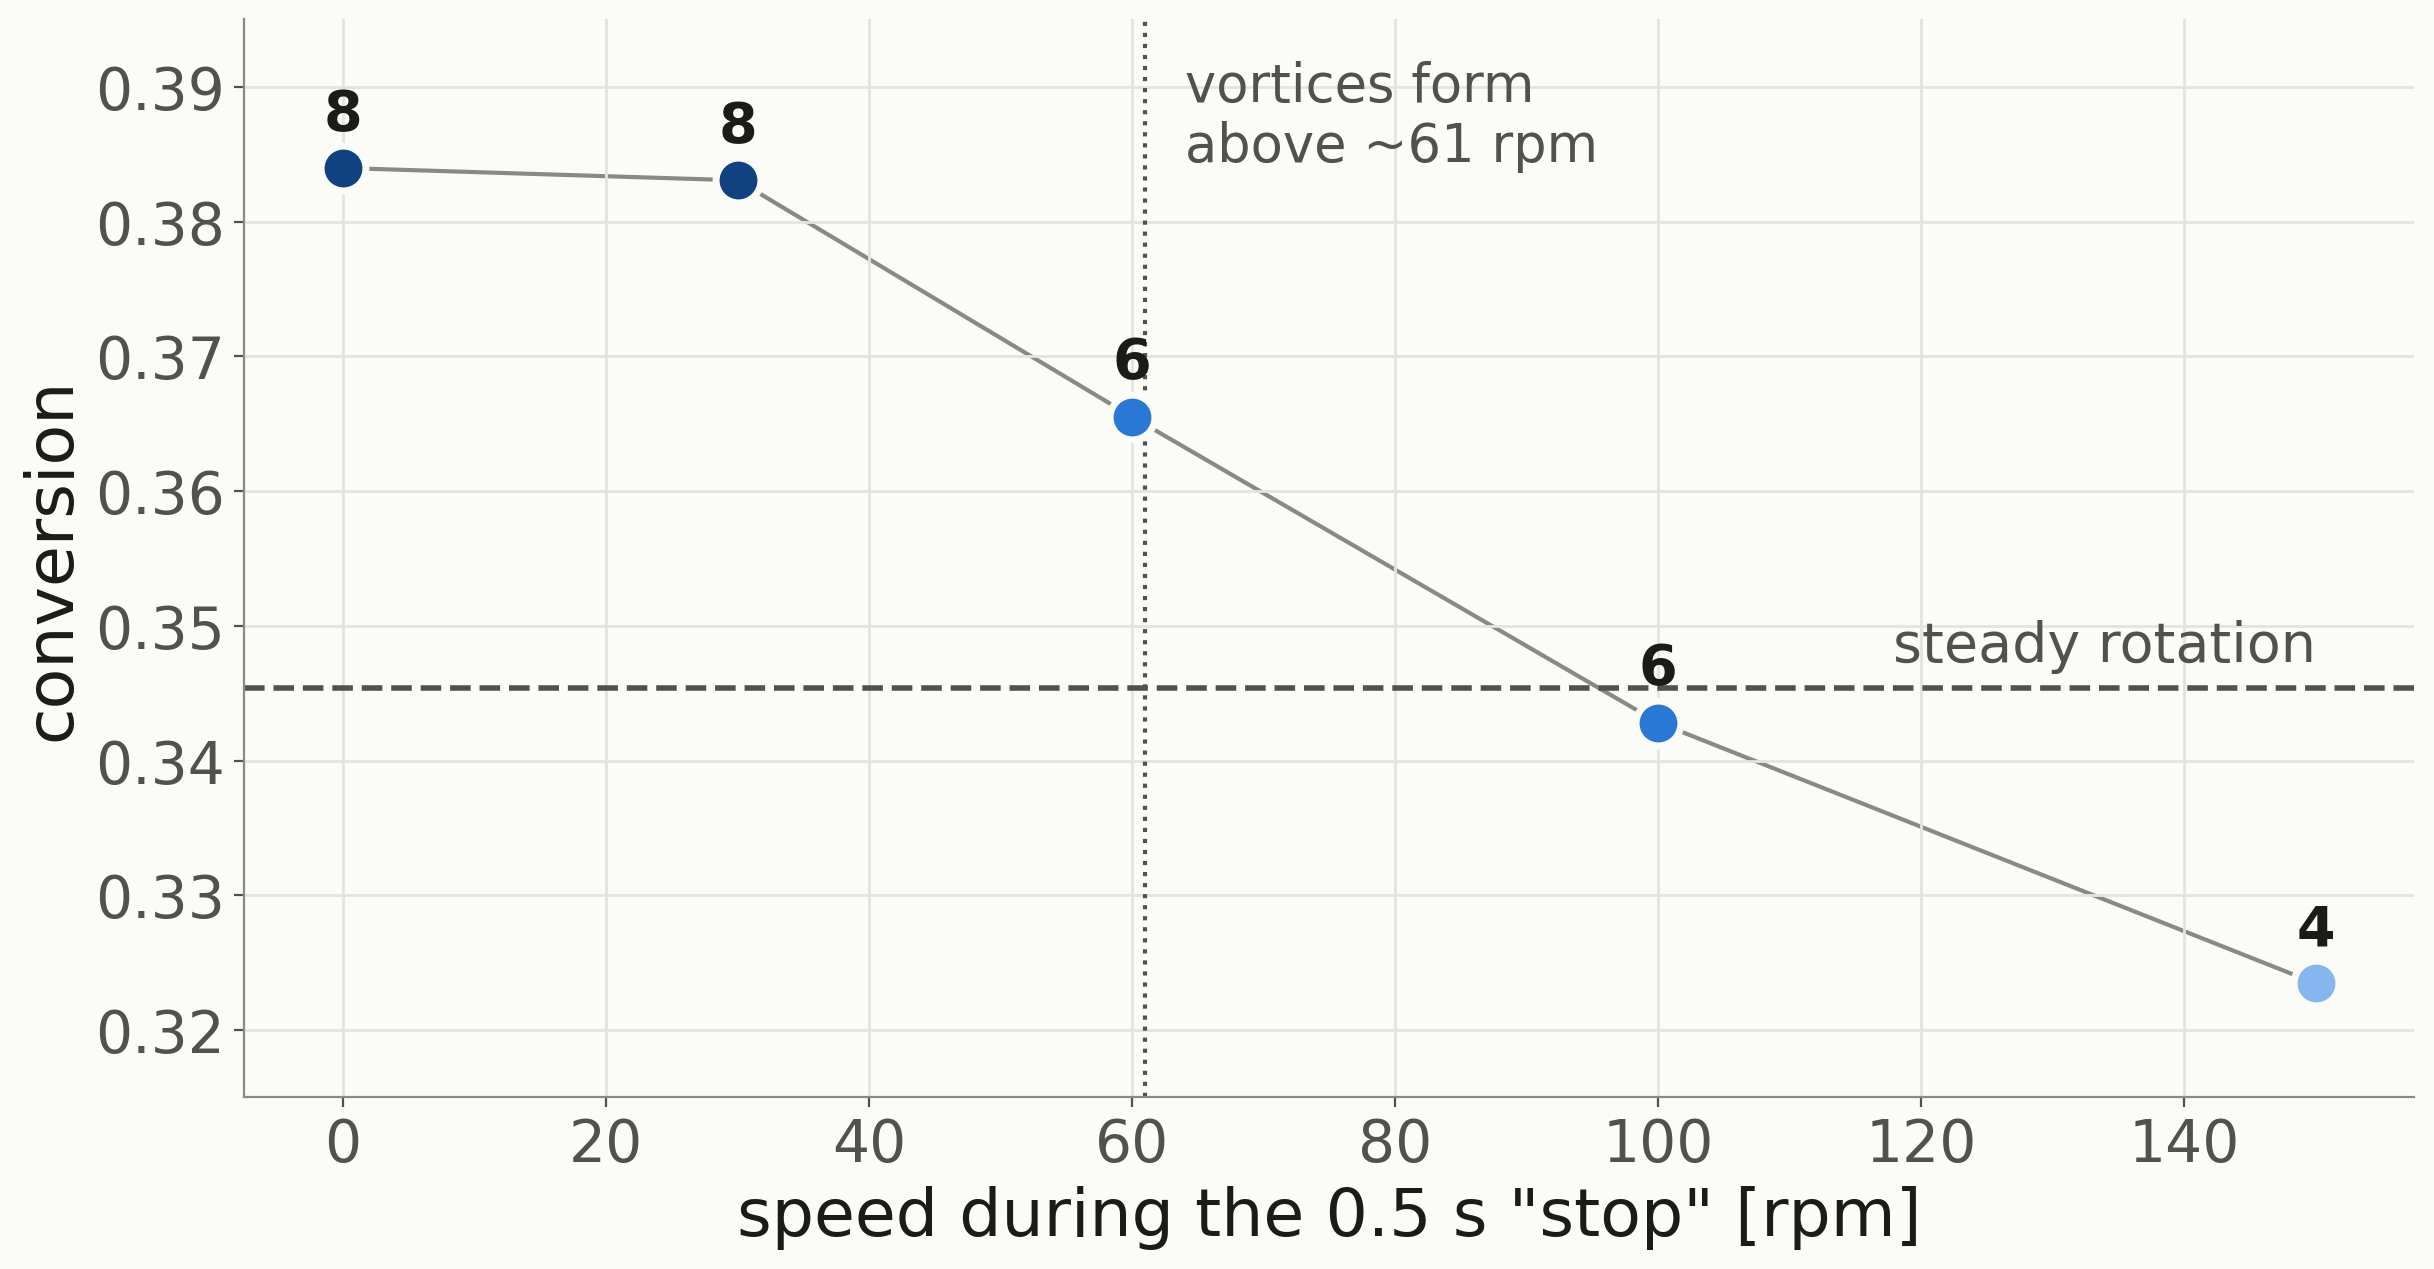
\includegraphics[width=\linewidth,height=0.76\textheight,keepaspectratio]{s_stop_level}
    \end{column}
    \begin{column}{0.30\textwidth}
      Vortices must die first.
    \end{column}
  \end{columns}
\end{frame}
\note{[0:30] Instead of stopping, I slowed the cylinder to 30, 60, 100 or 150 rpm for the same half second. Thirty is as good as a full stop. At 60 rpm, about where vortices start to form, you get six cells instead of eight, and at 100 and above the gain is gone. The vortices really have to die, to about one percent of their energy, before the restart can build a new, finer pattern.}

% ============================================================================
\begin{frame}{Conversion follows the cell count}
  \begin{columns}[c]
    \begin{column}{0.74\textwidth}
      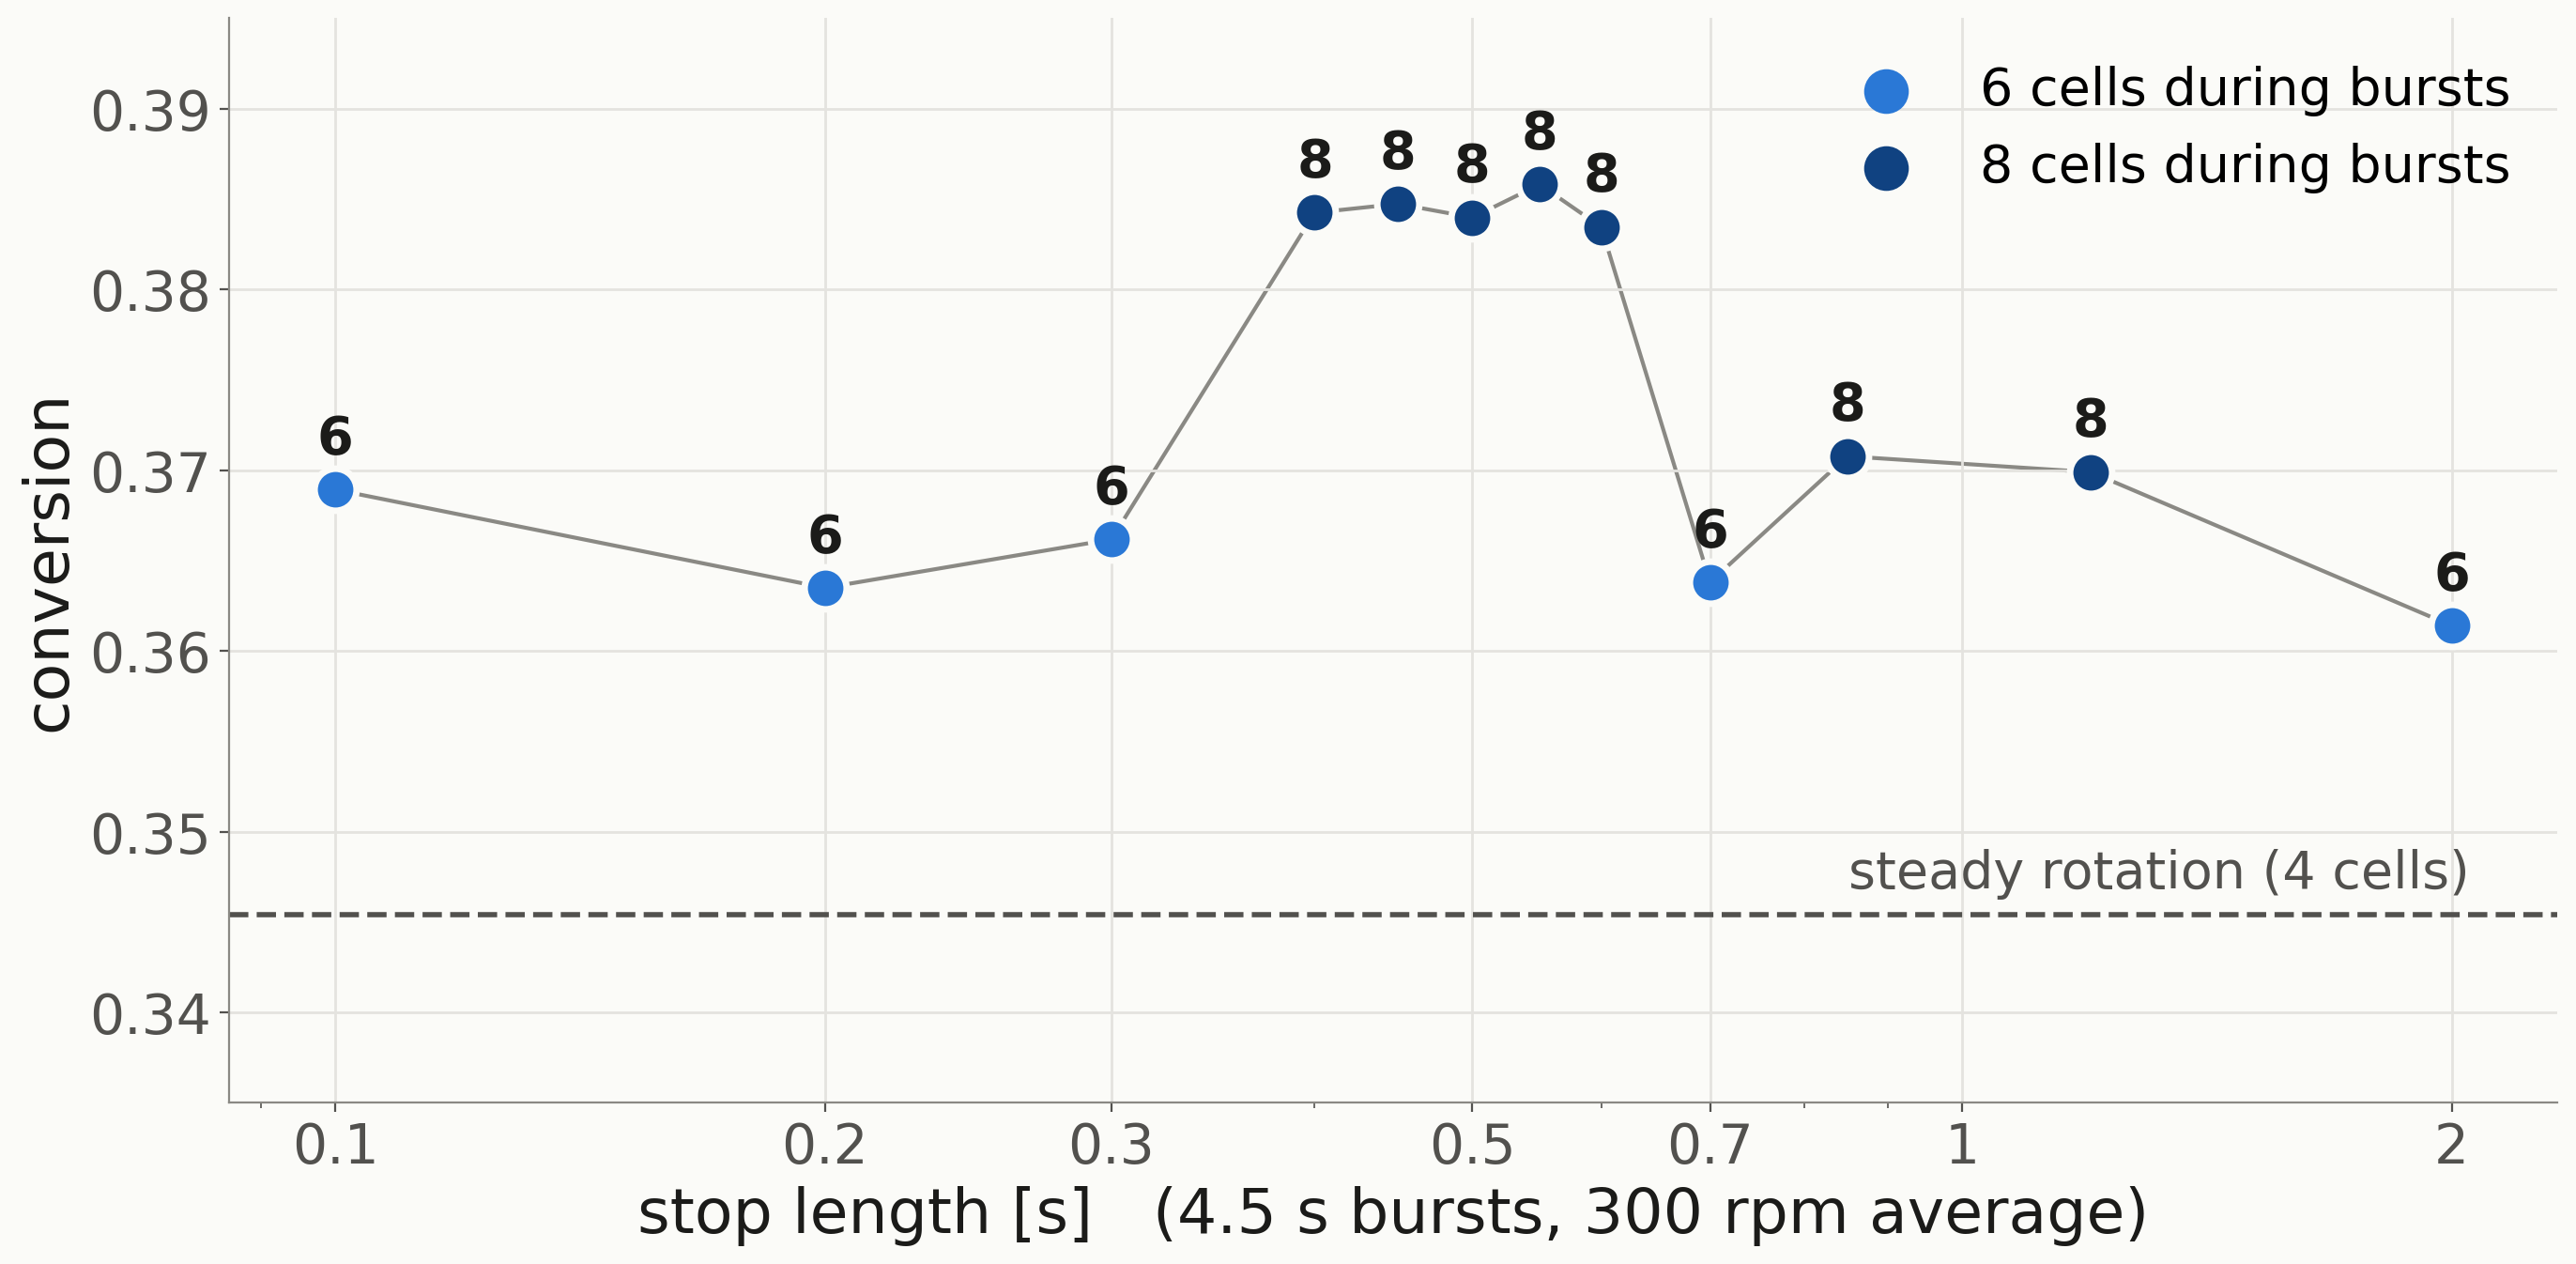
\includegraphics[width=\linewidth,height=0.74\textheight,keepaspectratio]{s_stop_curve_cells}
    \end{column}
    \begin{column}{0.24\textwidth}
      \bignum{+0.04}{conversion in the 8-cell window (0.4--0.6\,s stops)}\par\bigskip
      \bignum{4\,$\to$\,8}{cells, steady vs best pulsing}
    \end{column}
  \end{columns}
\end{frame}
\note{[0:45] Plot conversion against stop length and label each point with its cell count. It isn't a smooth curve with one peak; it's a set of levels. Steady rotation, four cells, at the bottom; six-cell stops in the middle; and the best stops, 0.4 to 0.6 seconds, are exactly the ones whose restart lands in eight cells, about 0.04 above steady rotation. The sudden drop at 0.7 seconds, which looked like a strange cliff in the original search, is just the flow falling back to six cells.}

% ============================================================================
\begin{frame}{Numerical verification}
  \begin{columns}[T]
    \begin{column}{0.58\textwidth}
      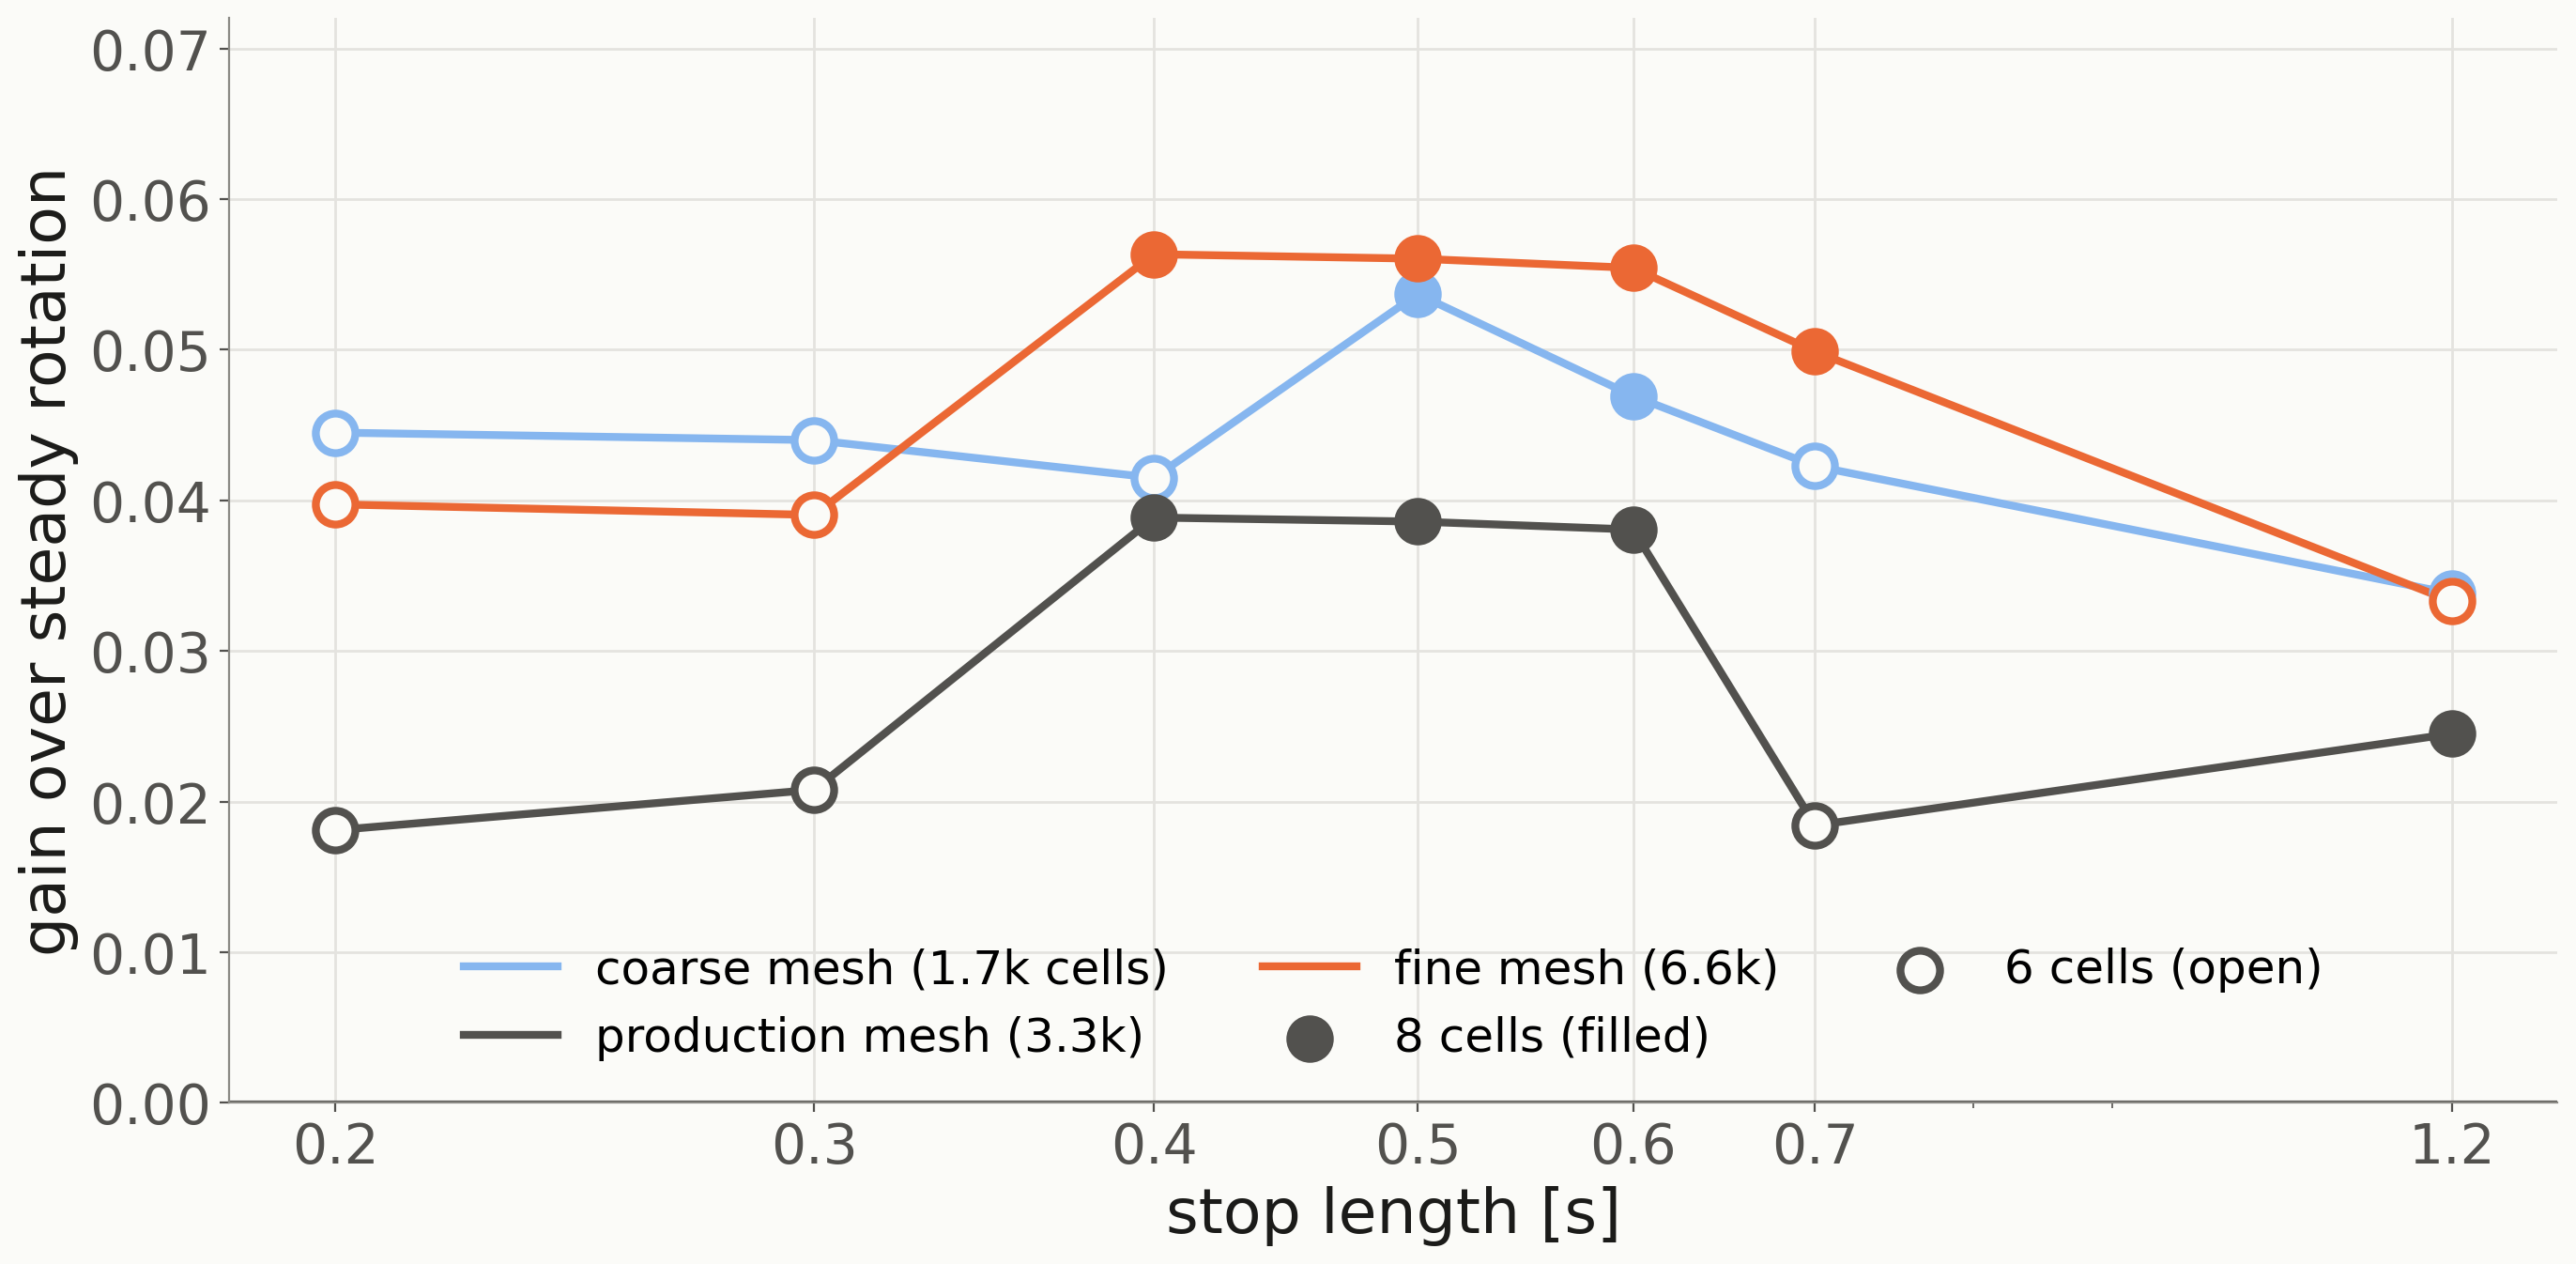
\includegraphics[width=\linewidth,height=0.62\textheight,keepaspectratio]{s_mesh_check}\par
      {\small\color{ink}3 meshes: same cells, gain +0.04 to +0.06}
    \end{column}
    \begin{column}{0.40\textwidth}
      \begin{block}{Checks}
        \begin{itemize}
          \item Half time step: outlet artifact gone
          \item Mass balance: 0.3\%
          \item Replicate noise: 0.002
        \end{itemize}
      \end{block}
    \end{column}
  \end{columns}
\end{frame}
\note{[0:45] For this audience the obvious question is whether it's numerics. I repeated the key runs on a coarser and a finer mesh from the same self-similar family. On all three, steady rotation has four cells, the best stops land in eight, and the gain is four to six hundredths. Halving the time step exposed and removed a spurious jet at the outlet worth about four hundredths of conversion, which is why all these runs use the smaller step. The mass balance closes to a third of a percent and replicate noise is about 0.002. What does move with the mesh is the exact edges of the eight-cell window, by a tenth of a second or two, so I quote ``about half a second''.}

% ============================================================================
\begin{frame}{Three takeaways}
  \begin{enumerate}
    \setlength\itemsep{0.8em}
    \item Brief full stops beat steady rotation and the published recipe.
    \item RL learns near-optimal control: matches 220-run optimization, transfers $5\times$ taller.
    \item Mechanism: restarts select more Taylor cells (8 vs 4); stops must repeat.
  \end{enumerate}
  \vfill
  {\small\color{ink}\textbf{Next:} messy conditions (feed, fluid drift) $\to$ feedback control; 3D check.\par\smallskip
  \textbf{Limits:} 2D axisymmetric; $\mathrm{Sc}=1075$.}
\end{frame}
\note{[0:45] One: brief full stops beat steady rotation at the same power, and beat the published recipe. Two: the RL pipeline learns near-optimal control from simulation alone. With no physics given, it matched an independent 220-run optimization, which is how we know it found the right answer, and it carried over to a reactor five times taller. Three: the optimum exploits multistability. Each restart selects a state with more cells that transports reactant faster, and because that state decays back under steady forcing, the stops have to repeat. This problem turned out to be simple: steady conditions, one best waveform, so a static optimizer can solve it too, and RL tying it is what you'd expect. The next step is to make it messy: changing feed rates and drifting fluid properties, where no fixed waveform stays right and a feedback policy should pull ahead. The main limit is the 2D model, so the mechanism is still a hypothesis for real 3D flow. Thank you, happy to take questions.}

% ============================================================================
\appendix
\begin{frame}{Backup: best fixed waveform vs the RL policy}
  \centering
  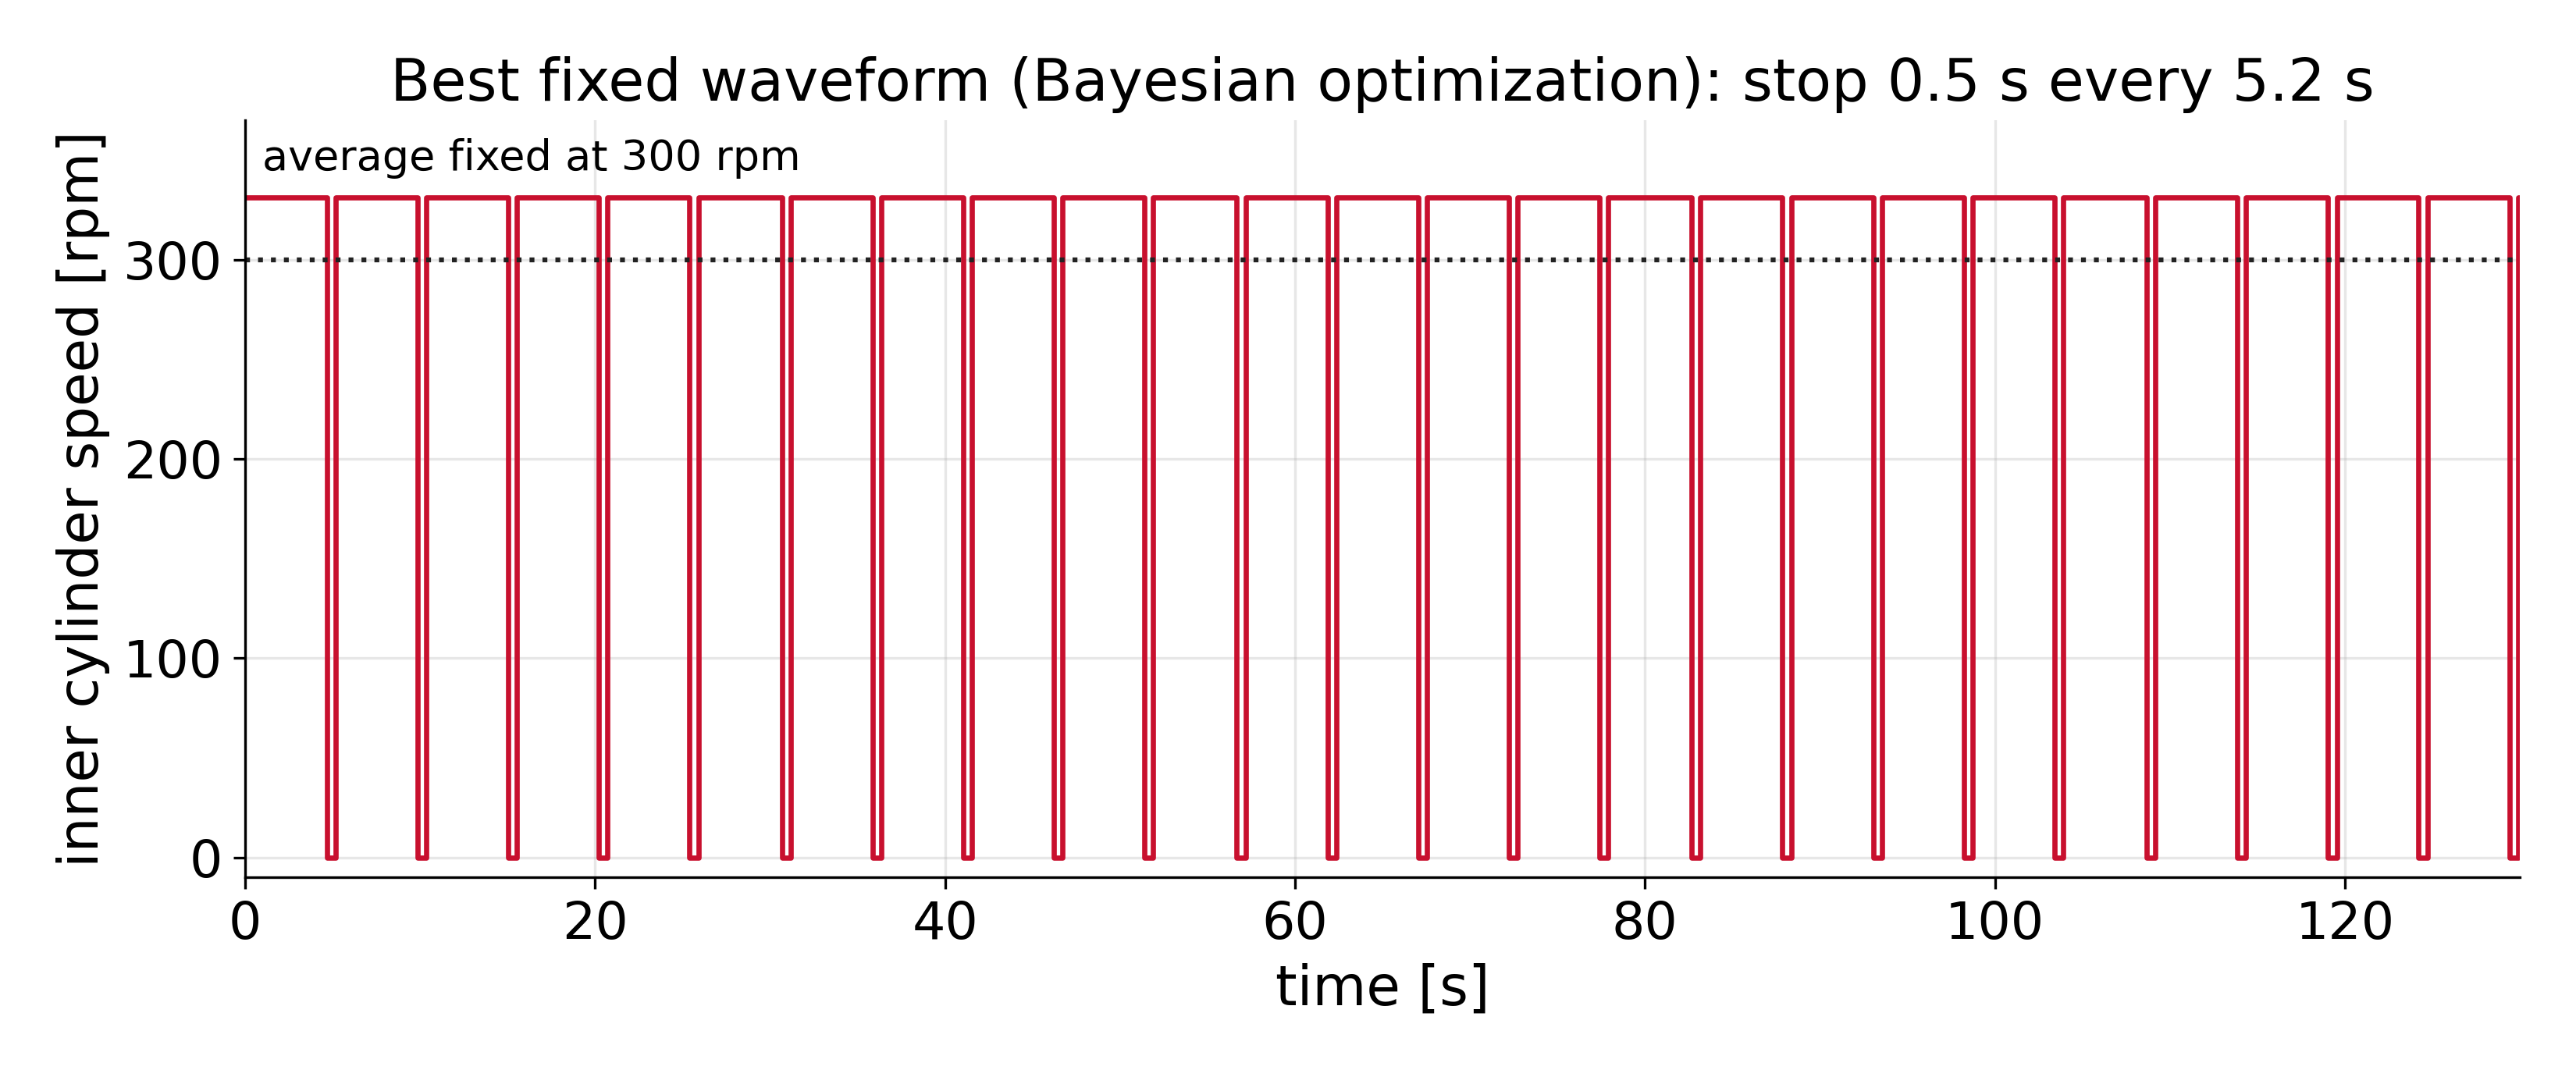
\includegraphics[width=0.86\linewidth,height=0.40\textheight,keepaspectratio]{bo_best_waveform}\par\smallskip
  \includegraphics[width=0.86\linewidth,height=0.40\textheight,keepaspectratio]{fig4_learned_waveform}
\end{frame}
\note{[Backup] Top: the best fixed waveform from the 220-run Bayesian optimization, stop half a second every five seconds, peak about 330 rpm. Bottom: what the RL policy chose. Same idea, brief full stops at high duty, but RL's stops are shorter, mostly a tenth to four tenths of a second, which mostly lands in the six-cell state and costs it one to two hundredths of conversion.}

% ============================================================================
\begin{frame}{Backup: why 0.5\,s? Two time scales, two predictions}
  \begin{columns}[T]
    \begin{column}{0.48\textwidth}
      \begin{block}{Swirl decay}
        \[ \tau = \frac{d^2}{\pi^2 \nu} \approx 0.4\ \mathrm{s} \]
        Slowest decay mode of momentum diffusion across the gap. Predicts best stop $\propto \nu^{-1}$.
      \end{block}
    \end{column}
    \begin{column}{0.48\textwidth}
      \begin{block}{Wall layer}
        \[ \tau = \frac{\delta^2}{D} \approx 0.8\ \mathrm{s} \]
        Regrowth of the depleted layer at the wall. At fixed $D$, predicts best stop $\propto \nu^{0.3}$ to $\nu^{0.7}$.
      \end{block}
    \end{column}
  \end{columns}
  \bigskip
  \takeaway{\textbf{Test:} vary $\nu$ at fixed $D$ and fit best stop $\propto \nu^{a}$. The sign of $a$ decides.}
\end{frame}
\note{[Backup] If asked whether a simple time scale explains the stop length: why half a second? Two time scales sit near it. One is the decay of the swirl: the slowest mode of momentum diffusion across a gap of width d decays on d squared over pi squared nu, about 0.4 seconds. The other is the time for the reactant-depleted layer at the wall to regrow, delta squared over D, about 0.8 seconds. They scale differently with viscosity. Holding the diffusivity fixed, the swirl clock predicts the best stop goes like nu to the minus one; the wall-layer clock predicts a positive power, about 0.3 to 0.7. So I varied the viscosity, fit an exponent, and decided in advance that its sign would pick the winner.}

% ============================================================================
\begin{frame}{Backup: neither guess sets the best stop}
  The swirl decays exactly as theory says (left), but the best stop follows neither prediction (right).\par\medskip
  \centering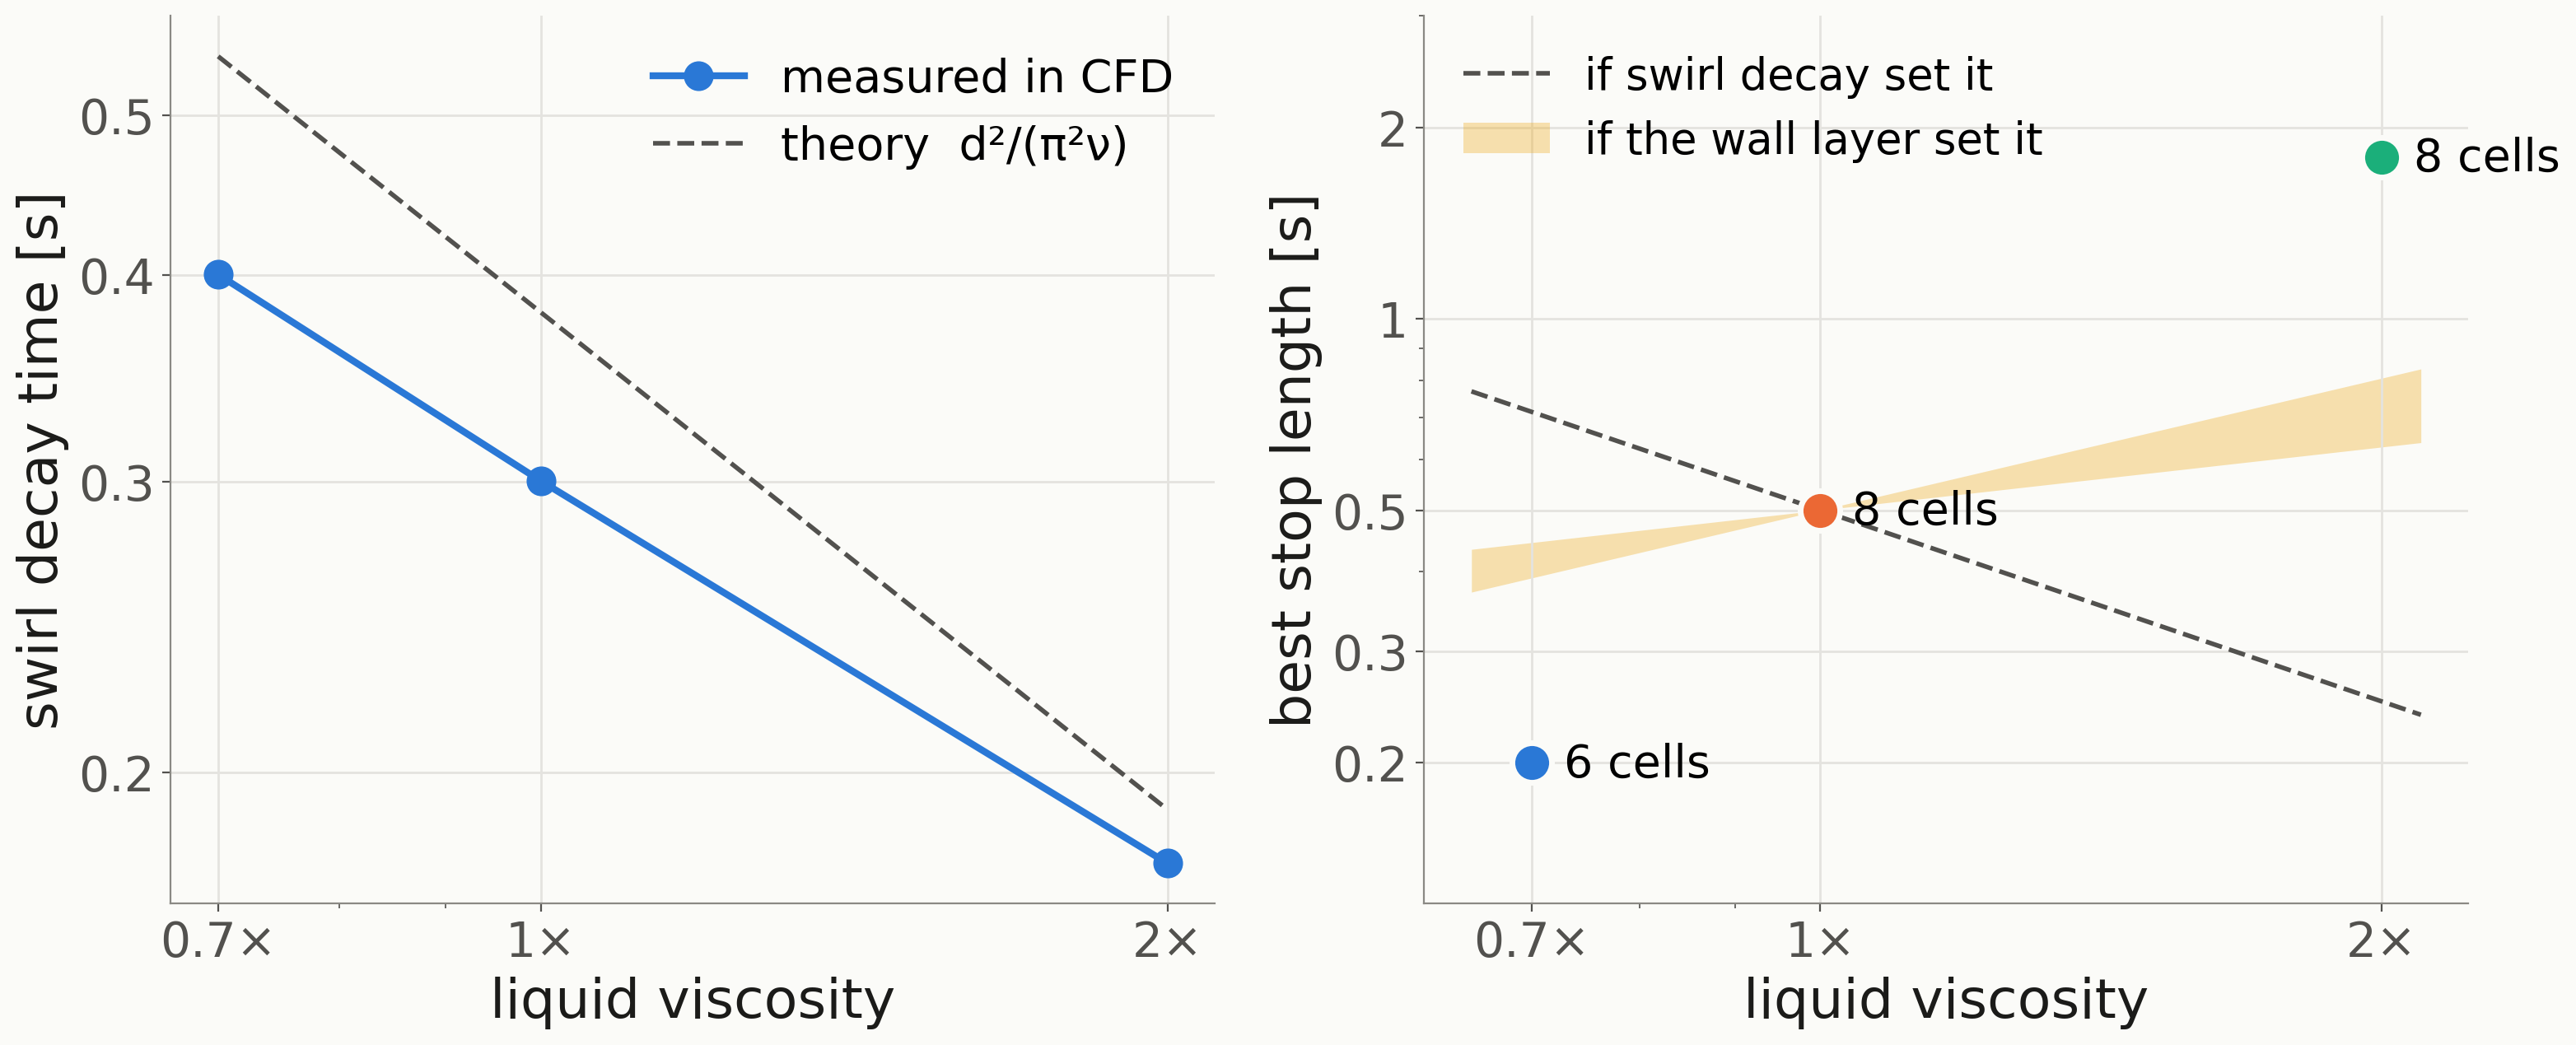
\includegraphics[width=\linewidth,height=0.66\textheight,keepaspectratio]{s_clocks}
\end{frame}
\note{[Backup] On the left, the swirl decays exactly as the eigenmode estimate says, one over viscosity. On the right, the best stop follows neither prediction; a formal exponent fit isn't even meaningful, because the optimum jumps rather than drifting. The labels, six cells and eight cells, are the clue.}


\begin{frame}{Backup: the gain is a higher plateau, not a restart spike}
  \centering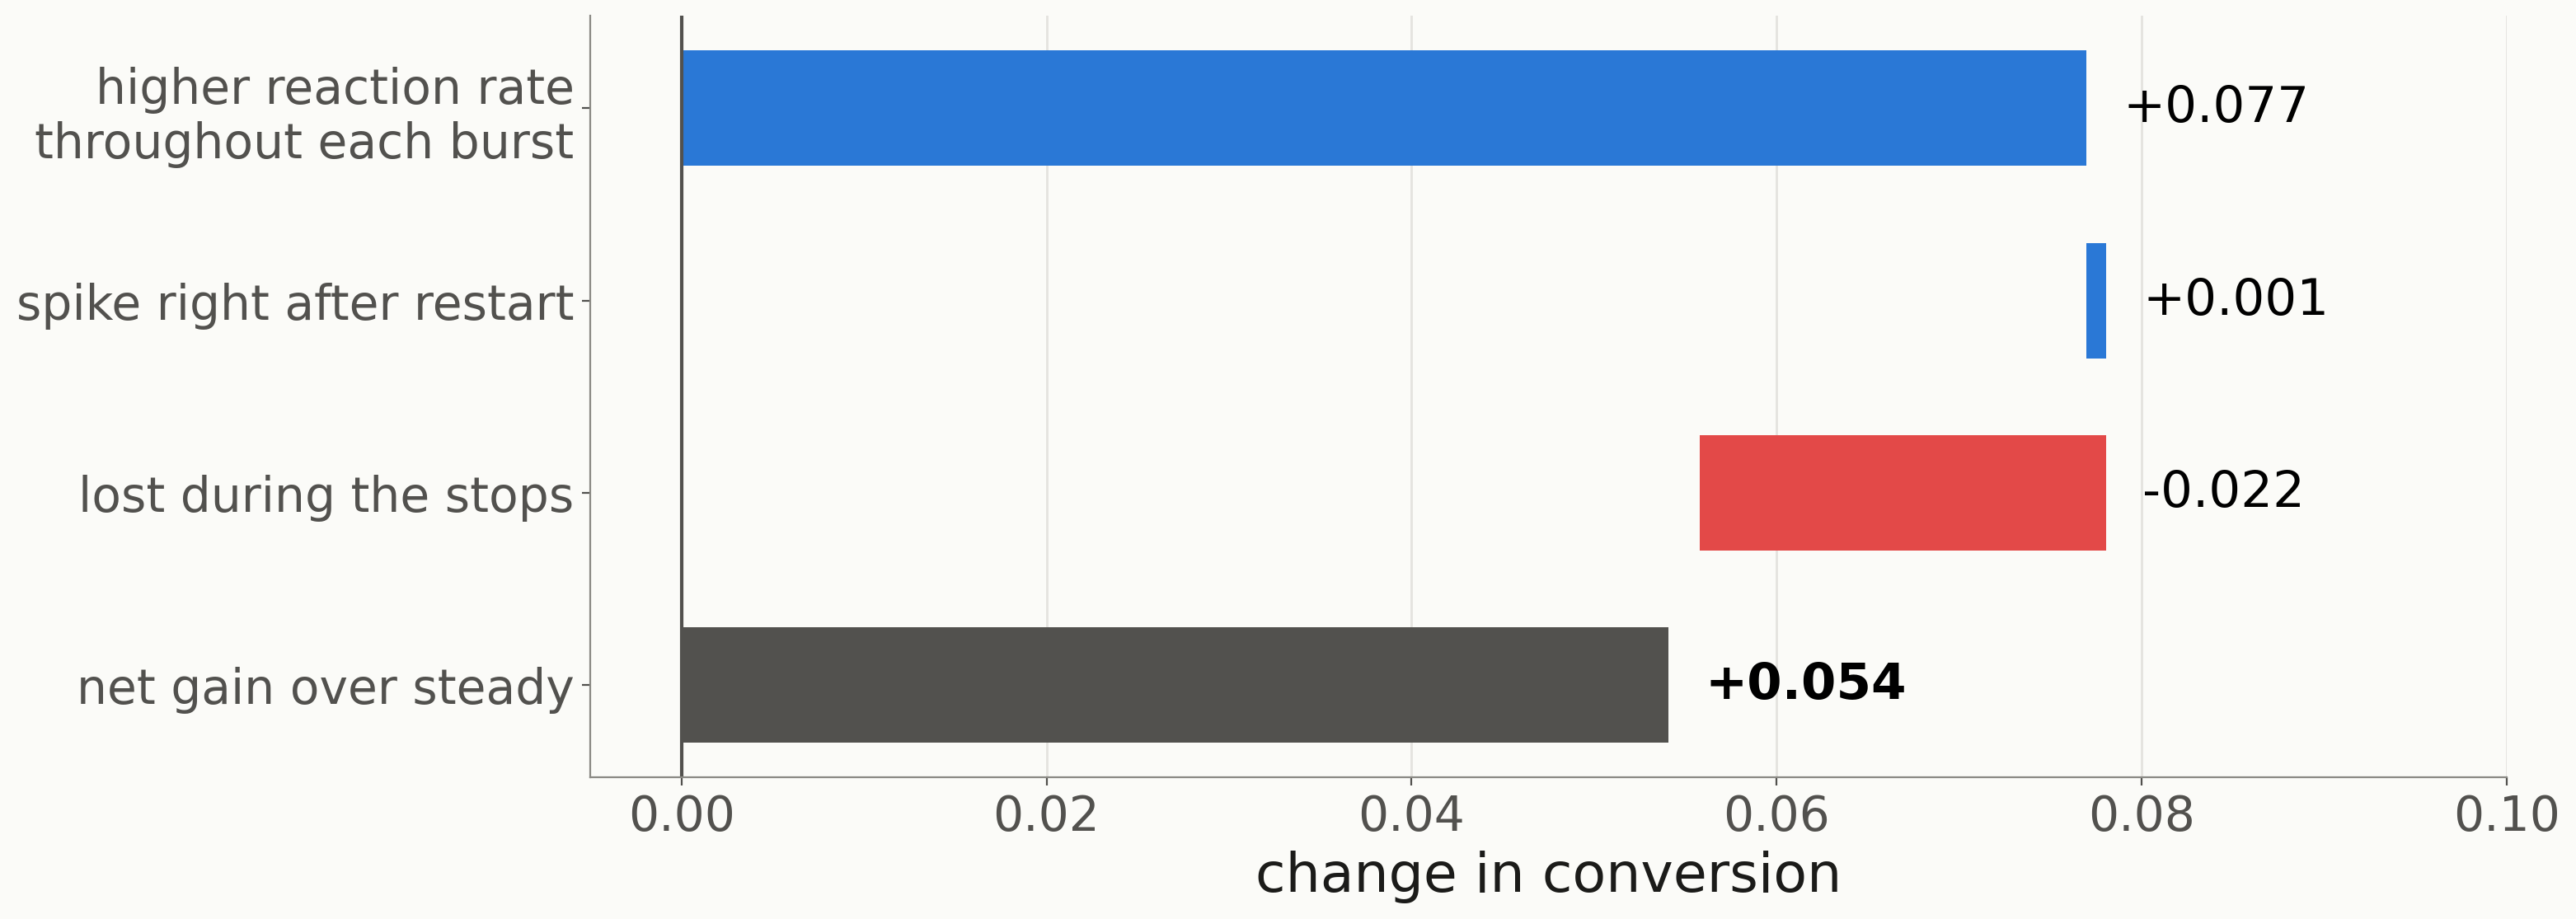
\includegraphics[width=\linewidth,height=0.62\textheight,keepaspectratio]{s_gain_breakdown}\par\smallskip
  \raggedright{\small\color{ink}From the wall-reaction traces of the best waveform's original run (wall-flux budget, last 26\,s).}
\end{frame}
\note{[Backup] If asked whether this is just a restart spike (``film renewal''): no. Splitting the gain over steady rotation: +0.077 from the reaction rate staying higher through the whole burst, only +0.001 from the spike right after restart, and $-0.022$ lost while stopped. The parts sum to 0.056 against the measured 0.054; the difference comes from how the burst plateau is defined.}

\begin{frame}{Backup: gain needs cells added over steady rotation}
  \begin{columns}[c]
    \begin{column}{0.64\textwidth}
      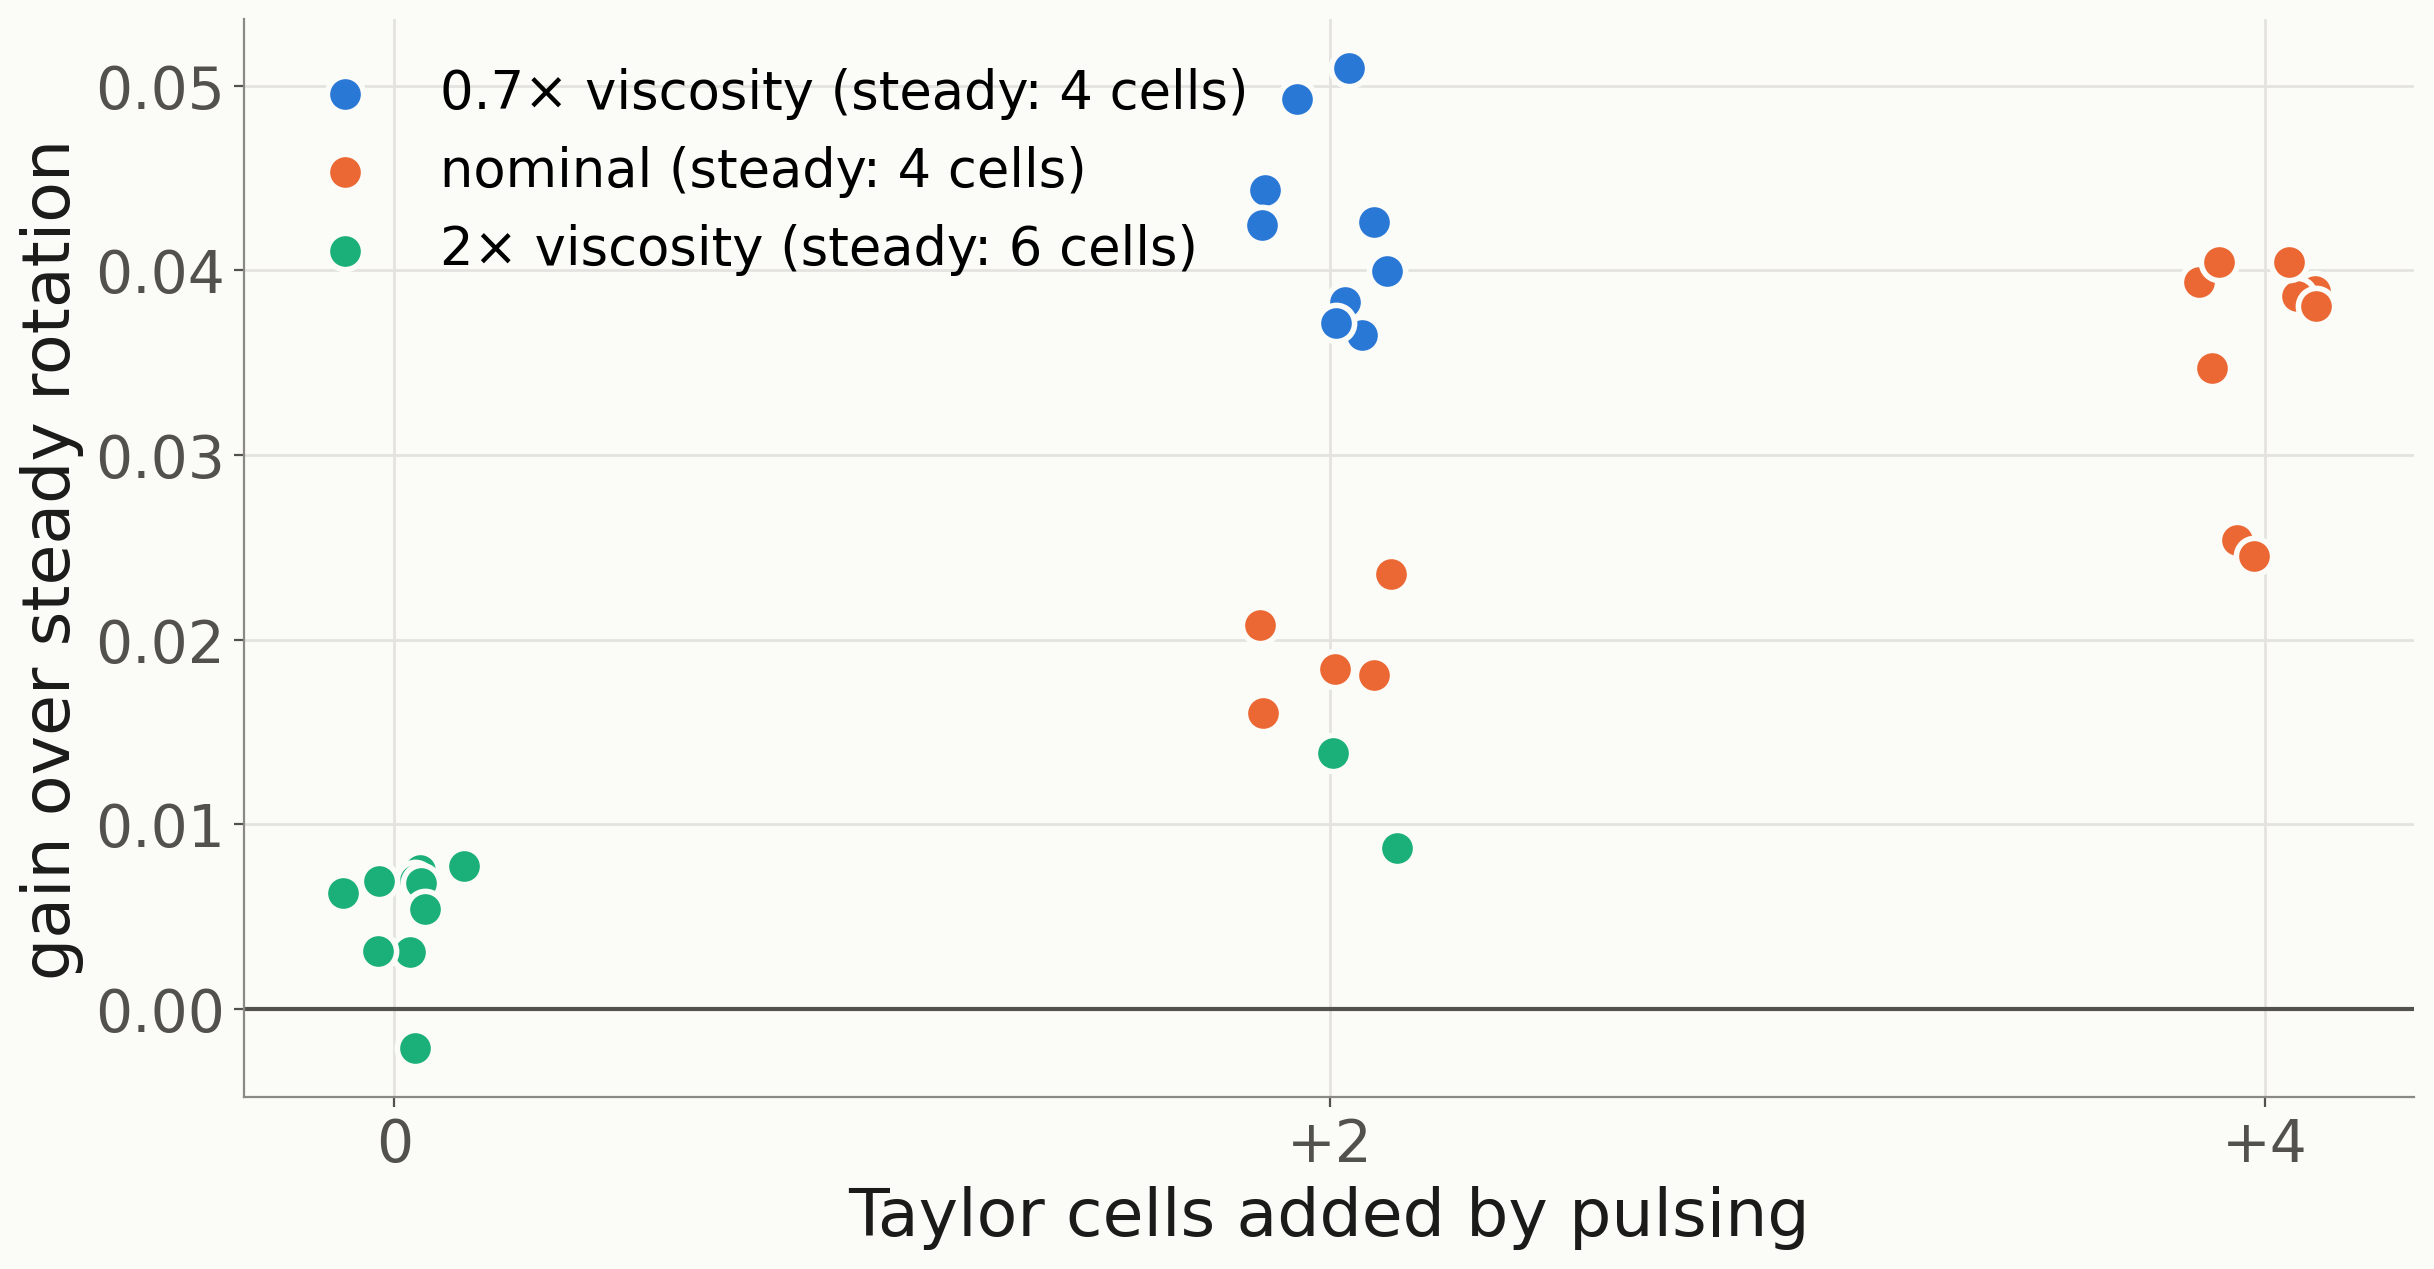
\includegraphics[width=\linewidth,height=0.72\textheight,keepaspectratio]{s_cells_added_gain}
    \end{column}
    \begin{column}{0.34\textwidth}
      At $2\times$ viscosity, steady rotation already holds 6 cells. Most pulses add none, and the gain shrinks to about +0.01.
    \end{column}
  \end{columns}
\end{frame}
\note{[Backup] Every pulsed run from the viscosity sweep, by how many cells pulsing adds over steady rotation at that viscosity. Runs that add no cells gain almost nothing; runs that add two or four gain up to five hundredths. At twice the viscosity steady rotation already has six cells, so most pulses add none. The size of the gain also depends on viscosity, so it isn't one universal curve.}

\begin{frame}{Backup: electrical power model}
  \begin{columns}[T]
    \begin{column}{0.58\textwidth}
      \begin{block}{L\'opez-Guajardo et al.\ (2024), \S3.4, Eqs.\ 18--23}
        {\small
        \[ T_{\mathrm{mot}} = \underbrace{J_{\mathrm{tot}}\,\dot\omega}_{\text{inertia}}
           + \underbrace{T_0\,\mathrm{sign}(\omega)}_{\text{bearings}}
           + \underbrace{\beta_2\,\omega^2\,\mathrm{sign}(\omega) + \beta_1\,\omega}_{\text{drag}} \]
        \[ i_{\mathrm{mot}} = \frac{T_{\mathrm{mot}}}{K_t}, \qquad
           e_{\mathrm{mot}} = L\,\frac{di_{\mathrm{mot}}}{dt} + R\,i_{\mathrm{mot}} + K_e\,\omega \]
        \[ P_{\mathrm{mot}} = e_{\mathrm{mot}}\, i_{\mathrm{mot}}, \qquad
           P_e = \begin{cases} P_{\mathrm{mot}}/\eta, & P_{\mathrm{mot}} \ge 0 \\ P_{\mathrm{mot}}\,\eta, & P_{\mathrm{mot}} < 0 \end{cases} \]}
      \end{block}
      {\small\color{ink}Evaluated on the commanded $\omega(t)$; reward uses $\overline{P_e}/P_{\max}$, $P_{\max} = 31.94$\,W (2500 rpm).}
    \end{column}
    \begin{column}{0.40\textwidth}
      {\small
      \begin{tabular*}{\linewidth}{@{}l@{\extracolsep{\fill}}r@{}}
        \toprule
        $J_{\mathrm{tot}}$ & $1.66\times10^{-4}$ kg\,m$^2$ \\
        $T_0$ & 0.1 N\,m \\
        $\beta_2$ & $7.19\times10^{-8}$ N\,m\,s$^2$ \\
        $\beta_1$ & $1.51\times10^{-5}$ N\,m\,s \\
        $K_t = K_e$ & 93.1 mN\,m/A \\
        $L$, \ $R$ & 0.28 mH, \ 0.178\,$\Omega$ \\
        $\eta$ & 0.90 \\ \bottomrule
      \end{tabular*}}\par\medskip
      {\small\color{ink}At 300 rpm the bearing term alone is $\approx$ 3.5 of the 3.7\,W, so power is set by the mean speed.}
    \end{column}
  \end{columns}
\end{frame}
\note{[Backup] The power model is the one L\'opez-Guajardo and colleagues used, Section 3.4 of their paper: motor torque from inertia, bearing friction and a quadratic drag fit; current from the torque constant; voltage from the armature circuit; electrical power with a 90 percent controller efficiency, and regeneration when braking. We evaluate it on the commanded speed and normalize by the power at 2500 rpm, 31.94 watts. At 300 rpm almost all of the 3.7 watts is bearing friction, which depends only on speed, so fixing the mean speed fixes the power, whatever the waveform's shape.}

\end{document}
"   (x2)
%                                                    -> talk_notes.pdf (slides + speaker notes)
% Figures: ../figures (make_slide_figures.py) and ../../poster_2026-10-02.
\documentclass[aspectratio=169,11pt]{beamer}
\usetheme{default}
\usepackage{lmodern}
\setbeamertemplate{navigation symbols}{}
\setbeamertemplate{blocks}[rounded][shadow=false]
\setbeamertemplate{footline}[frame number]
\setbeamertemplate{itemize items}[circle]
\usepackage[utf8]{inputenc}
\usepackage[T1]{fontenc}
\usepackage{amsmath,amssymb,bm}
\usepackage{booktabs}
\usepackage{tikz}
\usetikzlibrary{arrows.meta}
\graphicspath{{../figures/}{../../poster_2026-10-02/}{../../}}

\ifdefined\withnotes
  \setbeameroption{show notes}
  \setbeamertemplate{note page}[plain]
\fi

% ---- University of Houston palette (from the UH URD template) ---------------
% UH Red #C8102E, Brick #960C22, Slate #54585A; logos cut from the template's banner.
\definecolor{uhred}{HTML}{C8102E}
\definecolor{uhbrick}{HTML}{960C22}
\definecolor{uhslate}{HTML}{54585A}
\definecolor{navy}{HTML}{231F20}     % primary text (near-black)
\definecolor{ink}{HTML}{54585A}      % secondary text (UH slate)
\definecolor{accent}{HTML}{C8102E}
\definecolor{accentdk}{HTML}{960C22}
\definecolor{paper}{HTML}{FBFBF8}    % matches the figure backgrounds
\definecolor{card}{HTML}{F1F0EE}
\definecolor{vblue}{HTML}{1C5CAB}
\setbeamercolor{normal text}{fg=navy,bg=paper}
\setbeamercolor{frametitle}{fg=white,bg=uhred}
\setbeamercolor{alerted text}{fg=uhred}
\setbeamercolor{block title}{fg=uhbrick,bg=card}
\setbeamercolor{block body}{fg=ink,bg=card}
\setbeamercolor{structure}{fg=uhred}
\setbeamercolor{page number in head/foot}{fg=uhslate}
\setbeamerfont{block title}{size=\small,series=\bfseries}
\setbeamertemplate{frametitle}{%
  \nointerlineskip%
  \begin{beamercolorbox}[wd=\paperwidth,ht=7.5mm,dp=2.8mm,leftskip=4.5mm,rightskip=3.5mm]{frametitle}%
    \usebeamerfont{frametitle}\insertframetitle\hfill\raisebox{-1.7mm}{
\includegraphics[height=6.2mm]{uh/uh_mark_white}}%
  \end{beamercolorbox}%
  \vspace{1mm}}

\newcommand{\takeaway}[1]{\par\smallskip{\color{ink}#1}\par}
\newcommand{\bignum}[2]{{\usebeamerfont{title}\color{navy}\LARGE\bfseries #1}\\[-1pt]{\small\color{ink}#2}}

\title{Brief stops, more vortices}
\subtitle{Deep reinforcement learning discovers transferable control strategies for catalytic-wall Taylor--Couette reactors}
\author{Isaiah N.\ Bascom\inst{1} \and Min Wang\inst{1} \and Yuhe Wang\inst{2}}
\institute{\inst{1}Department of Mathematics, University of Houston, Houston, Texas \and \inst{2}Institute for Scientific Computation, Texas A\&M University, College Station, Texas}
\date{GCURS 2026 \textbullet\ Computational \& Applied Mathematics}

\begin{document}

% ============================================================================
\begin{frame}[plain]
  \begin{tikzpicture}[remember picture,overlay]
    \fill[uhred] (current page.north west) rectangle ([yshift=-15mm]current page.north east);
    \node[anchor=west] at ([xshift=6mm,yshift=-7.5mm]current page.north west) {
\includegraphics[height=9.5mm]{uh/uh_mark_white}};
    \node[anchor=east] at ([xshift=-6mm,yshift=-7.5mm]current page.north east) {
\includegraphics[height=10.5mm]{uh/uh_wordmark_white}};
    \node[anchor=center, text=white, font=\scriptsize\bfseries] at ([yshift=-7.5mm]current page.north) {GCURS 2026 \textbullet\ COMPUTATIONAL \& APPLIED MATHEMATICS};
    \node[anchor=north west, text width=148mm, align=left, inner sep=0pt, text=navy, font=\usebeamerfont{title}\huge\bfseries]
      at ([xshift=6mm,yshift=-20mm]current page.north west) {Brief stops, more vortices};
    \node[anchor=north west, inner sep=0pt, text=ink]
      at ([xshift=6mm,yshift=-31mm]current page.north west) {\resizebox{148mm}{!}{Deep reinforcement learning discovers transferable control strategies for catalytic-wall Taylor--Couette reactors}};
    \node[anchor=north, inner sep=0pt] at ([yshift=-40mm]current page.north)
      {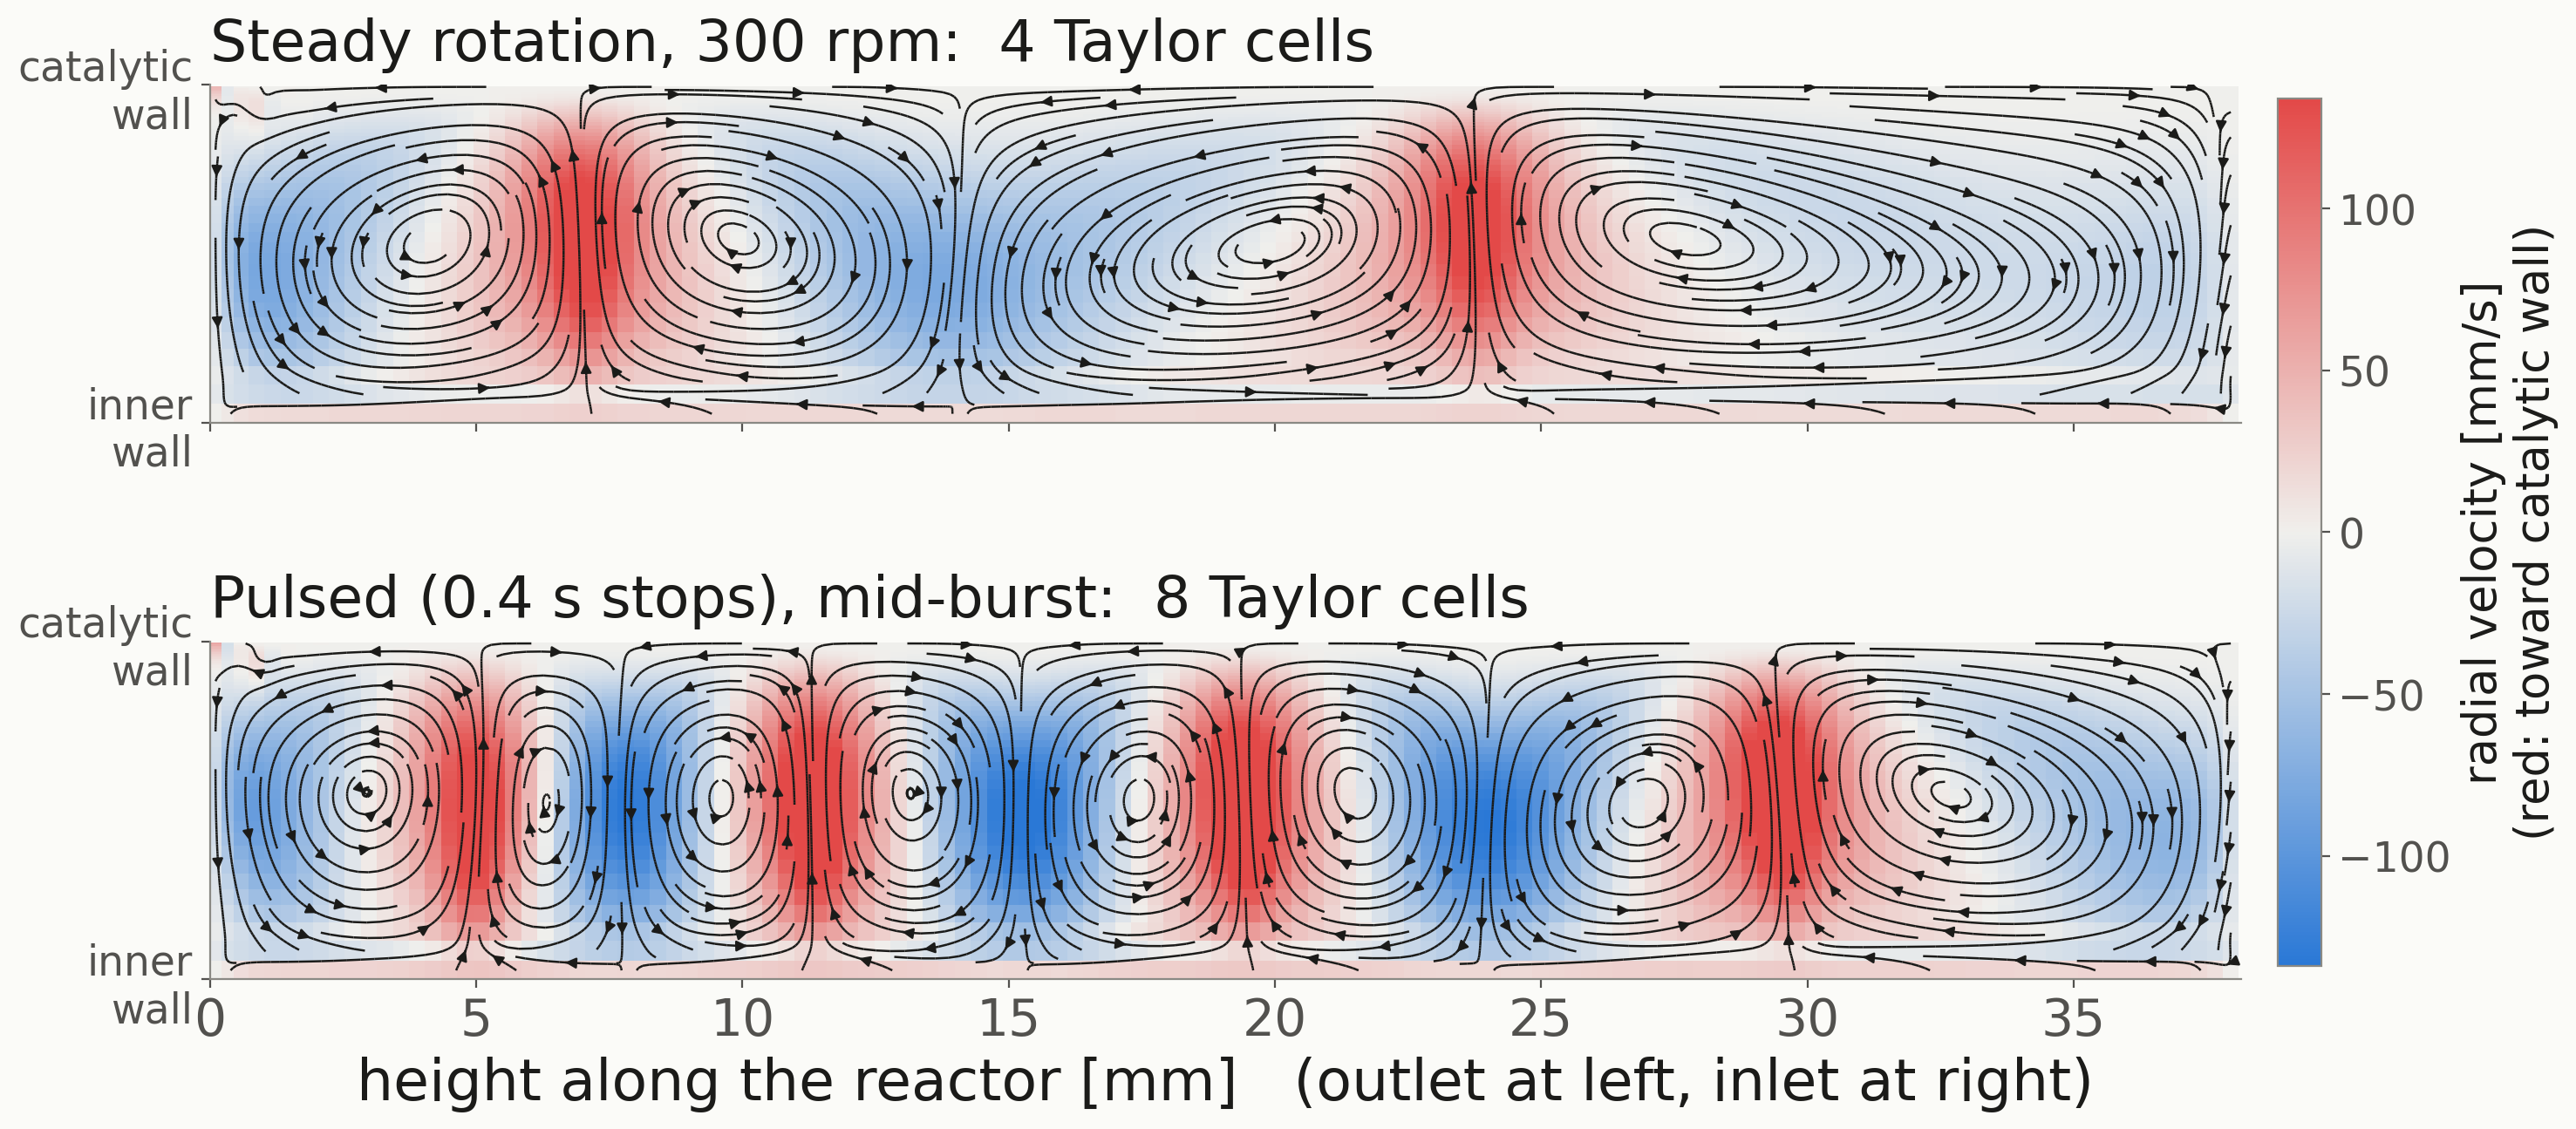
\includegraphics[width=148mm,height=30mm,keepaspectratio]{s_cells_snapshot}};
    \node[anchor=south west, inner sep=0pt, text=navy, font=\bfseries] at ([xshift=6mm,yshift=11.5mm]current page.south west)
      {Isaiah N.\ Bascom$^{1}$, \ Min Wang$^{1}$, \ Yuhe Wang$^{2}$};
    \node[anchor=south west, inner sep=0pt, text=ink, font=\scriptsize, align=left] at ([xshift=6mm,yshift=4mm]current page.south west)
      {$^{1}$Department of Mathematics, University of Houston, Houston, Texas\\
       $^{2}$Institute for Scientific Computation, Texas A\&M University, College Station, Texas};
  \end{tikzpicture}
\end{frame}
\note{[0:30] Hi, I'm Isaiah Bascom. I work on Taylor--Couette reactors: a liquid fills the gap between two cylinders, the inner one spins, and a catalyst coats the outer wall. Today's story has two parts. First, a reinforcement-learning agent found a surprisingly simple way to run this reactor better: brief full stops. Second, we found out why it works. The picture is the punchline: steady rotation gives four vortex cells, and pulsed rotation gives eight.}

% ============================================================================
\begin{frame}{The Taylor--Couette reactor}
  \begin{columns}[c]
    \begin{column}{0.60\textwidth}
      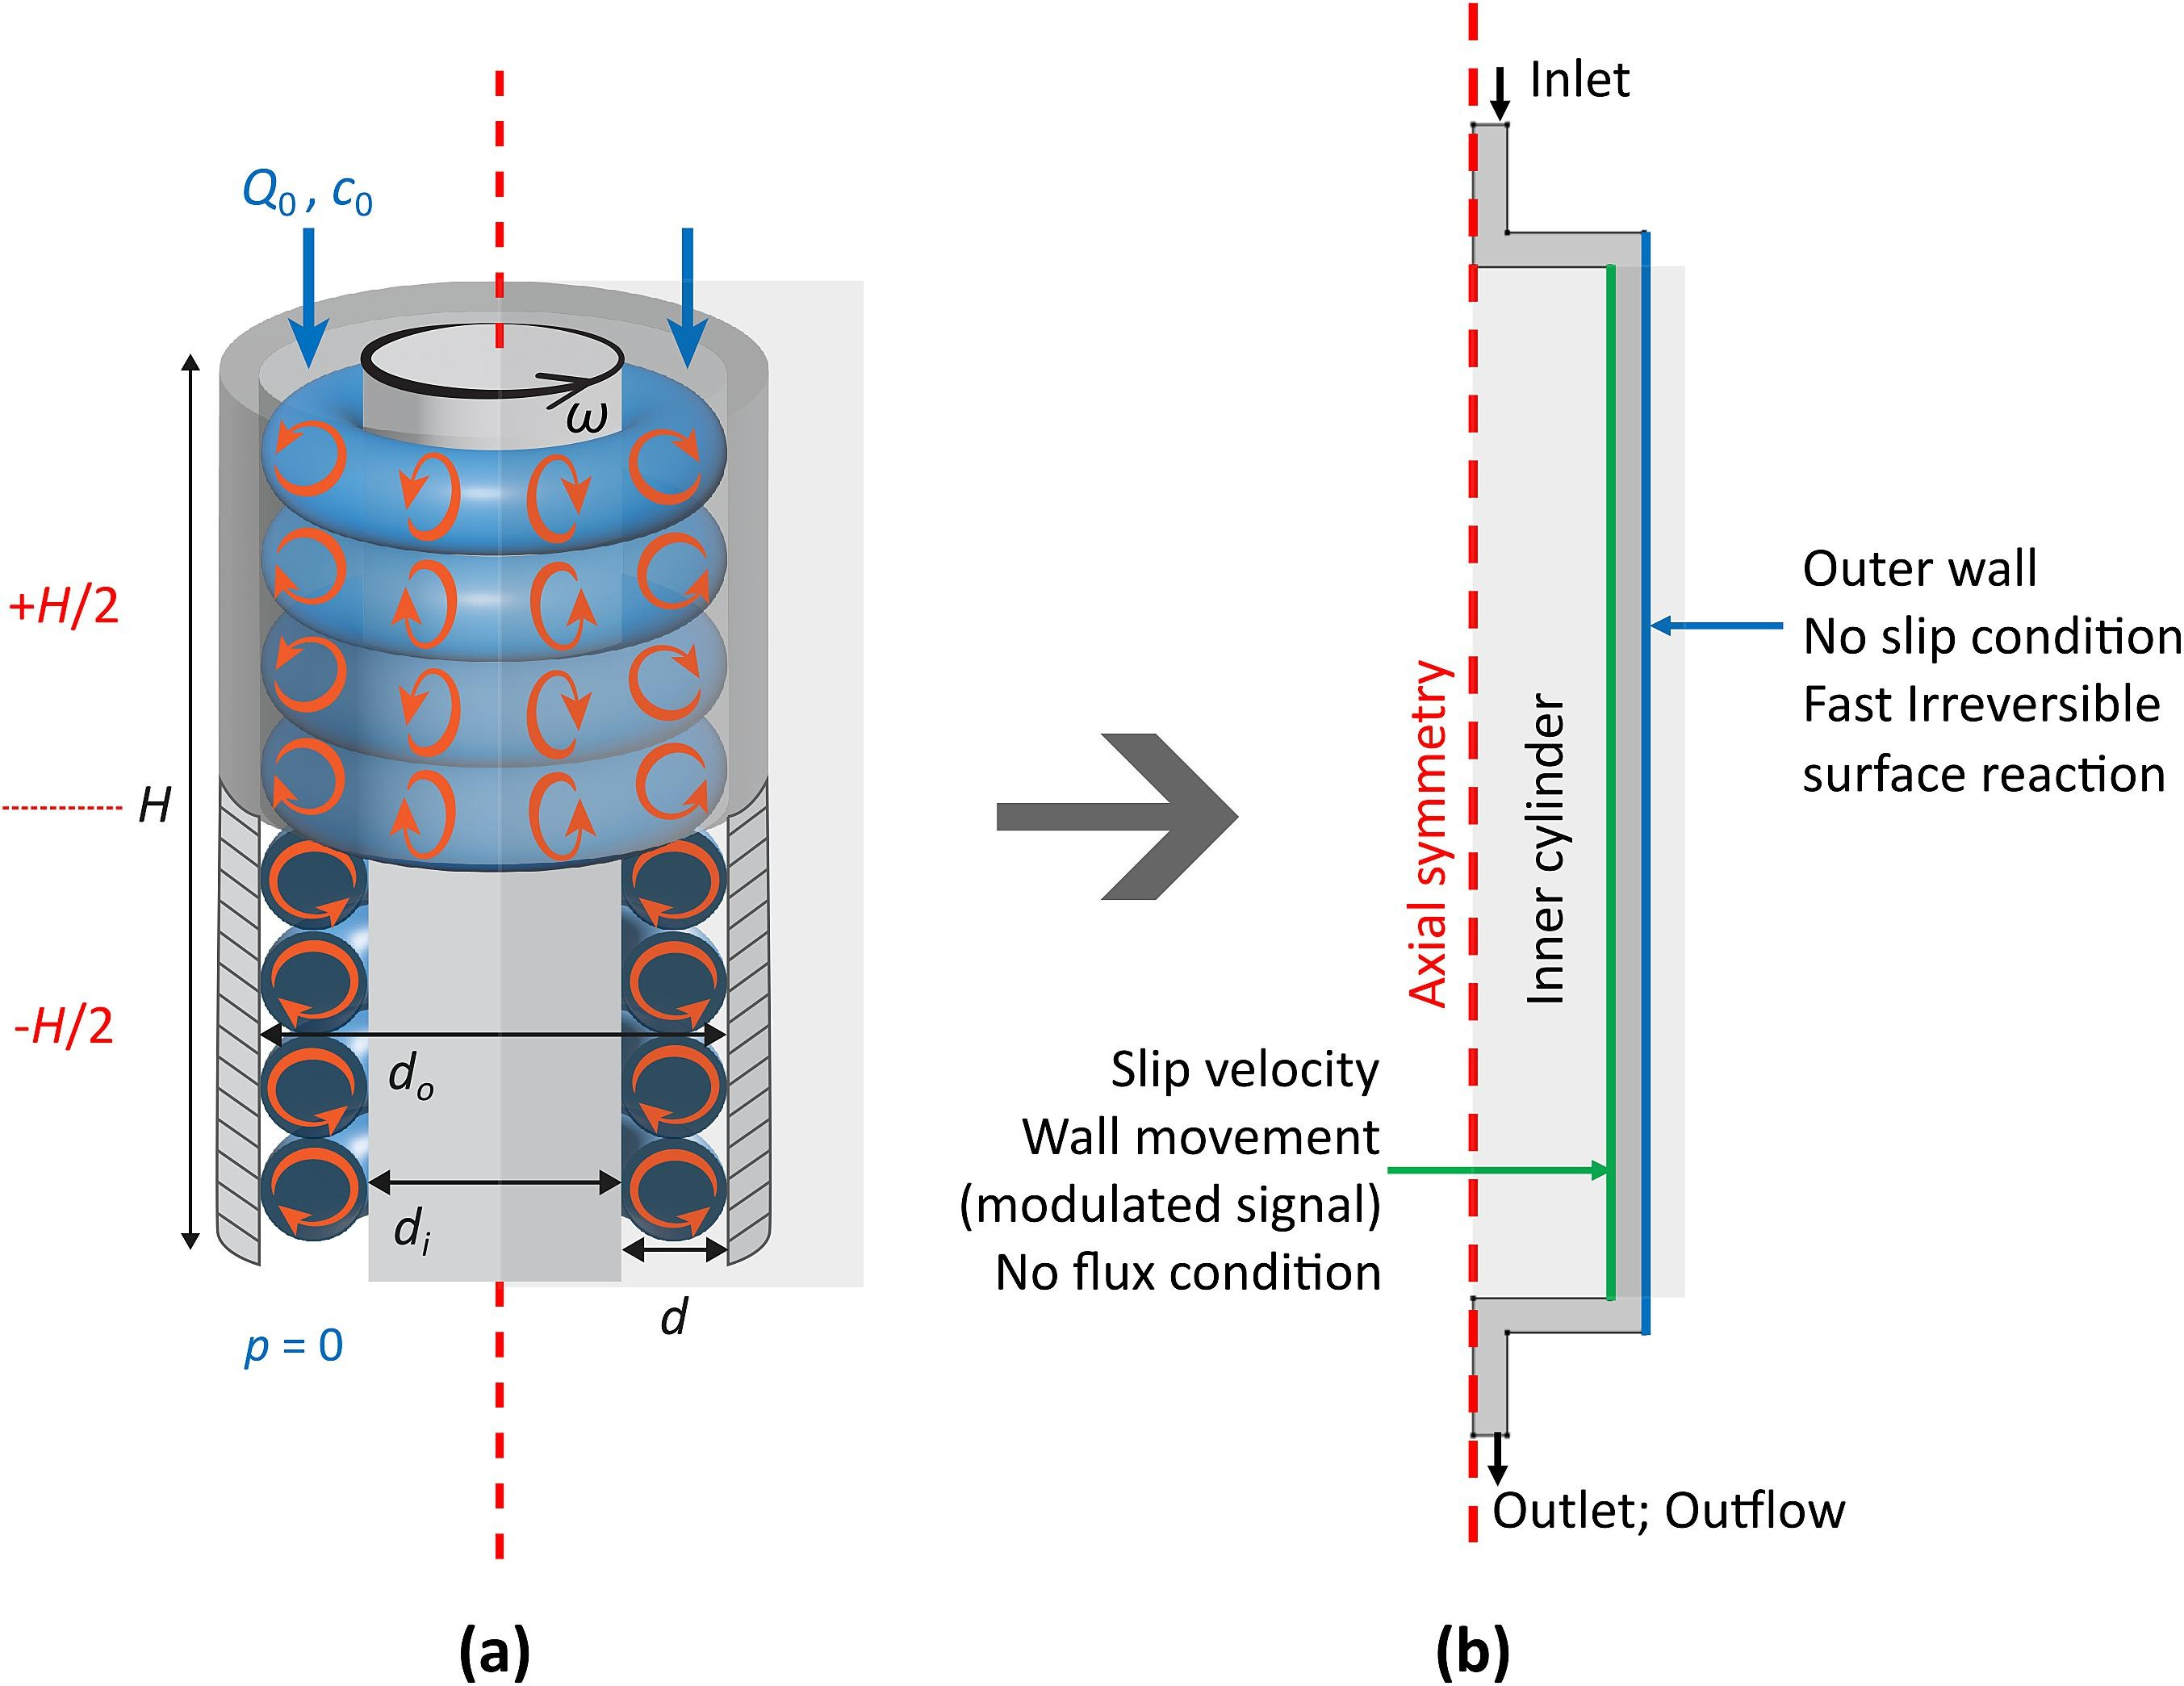
\includegraphics[width=\linewidth,height=0.78\textheight,keepaspectratio]{lg-reactor}\par
      {\tiny\color{ink}Figure: L\'opez-Guajardo et al., \emph{Chem.\ Eng.\ J.} 489 (2024) 151174, Fig.~2.}
    \end{column}
    \begin{column}{0.36\textwidth}
      {\small
      \begin{tabular*}{\linewidth}{@{}l@{\extracolsep{\fill}}r@{}}
        \toprule
        Gap $d$ & 6.35 mm \\
        $d_i$ / $d_o$ & 50.8 / 63.5 mm \\
        Height $H$ & 190.5 mm \\
        $\Gamma = H/d$ & 30 \\
        Feed $Q_0$ & 100 mL/min \\ \bottomrule
      \end{tabular*}}\par\bigskip
      Inner cylinder spins; catalyst on the outer wall.
    \end{column}
  \end{columns}
\end{frame}
\note{[0:45] First, the general setup. A Taylor--Couette reactor is liquid in the gap between two cylinders. The inner one spins, which sets up the stacked ring vortices you see on the left, the Taylor vortices. Feed enters at the top and leaves at the bottom, and the outer wall is coated with catalyst, so the reaction happens only there. The gap is about six millimetres, the reactor is about nineteen centimetres tall, an aspect ratio of thirty. Because the flow is symmetric around the axis, we can simulate just a two-dimensional slice, shown on the right; that's the standard reduction, and it's what makes reinforcement learning on this problem affordable.}

% ============================================================================
\begin{frame}{The reaction happens only at the wall}
  \begin{columns}[c]
    \begin{column}{0.52\textwidth}
      Taylor vortices carry reactant to the catalytic wall.\par\bigskip
      \begin{block}{Problem}
        Choose $\omega(t)$ for the most conversion per unit power.
      \end{block}
    \end{column}
    \begin{column}{0.46\textwidth}
      \centering
      % 2D axisymmetric domain (cf. Lopez-Guajardo et al. Fig. 2b): the fluid gap is the
      % real CFD field under the learned RL policy; everything else is drawn.
      \begin{tikzpicture}[x=1mm, y=1mm, every node/.style={font=\scriptsize}]
        \def\H{46}            % drawn height of the gap [mm]; width = H/6 (true 6.35:38.1)
        \def\W{7.67}
        \def\xg{14}           % left edge of the fluid gap
        % axis of symmetry
        \draw[uhred, dashed, line width=0.8pt] (0,-3) -- (0,\H+4);
        \node[rotate=90, text=uhred, font=\tiny] at (-2.2,\H/2) {axis of symmetry};
        % inner cylinder (schematic, not to scale in r)
        \fill[black!25] (3,0) rectangle (\xg,\H);
        \node[rotate=90, align=center, font=\tiny] at (8.5,\H/2) {inner cylinder, $\omega(t)$};
        % fluid gap: real field
        \node[anchor=south west, inner sep=0] at (\xg,0) {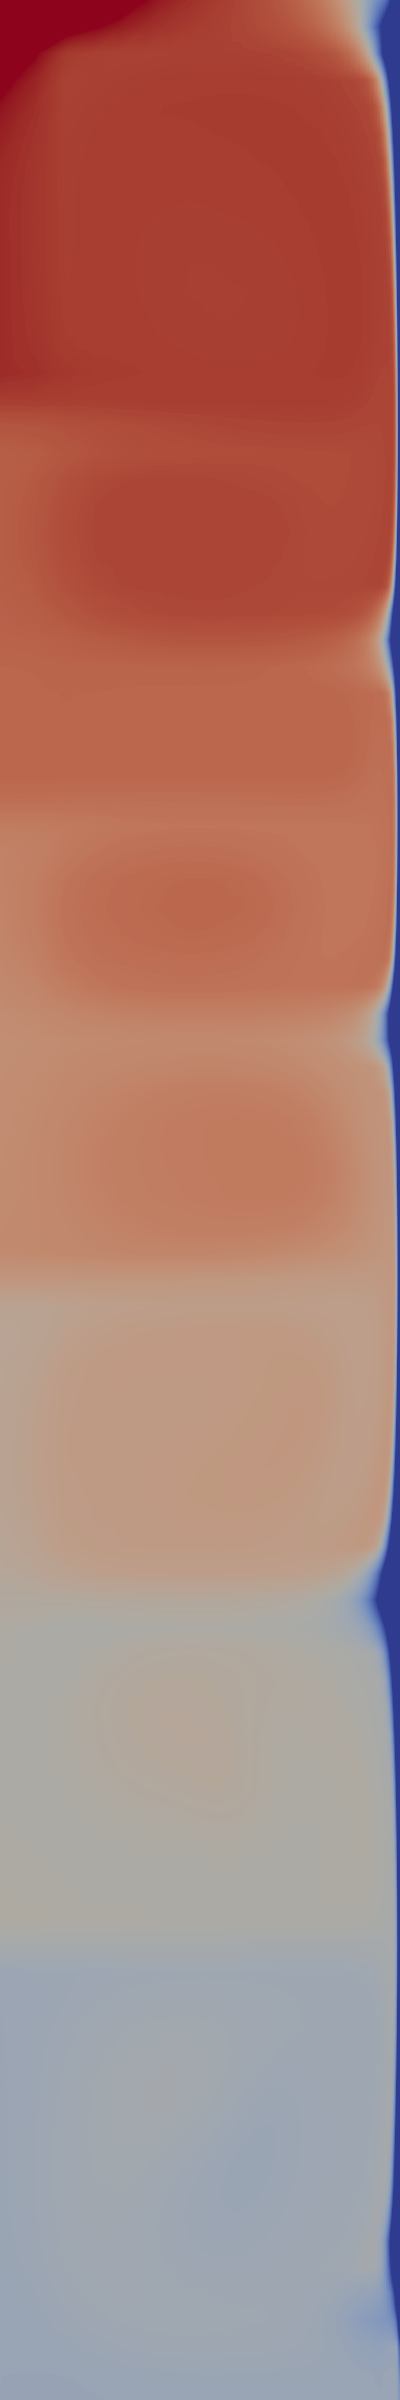
\includegraphics[width=\W mm,height=\H mm]{rl_flow_2d_conc_crop}};
        % bottom wall and catalytic outer wall (outer wall stops above the side outlet)
        \draw[black!60, line width=1.2pt] (\xg,0) -- (\xg+\W,0);
        \definecolor{wallblue}{HTML}{3B4CC0}   % bottom of the concentration scale: c = 0
        \draw[wallblue, line width=1.6pt] (\xg+\W+0.6,1.4) -- (\xg+\W+0.6,\H);
        % inlet at the top of the gap
        \draw[-{Latex[length=2mm]}, navy, line width=1pt] (\xg+\W/2,\H+6) -- (\xg+\W/2,\H+0.6);
        \node[anchor=south] at (\xg+\W/2,\H+6) {inlet};
        % side outlet: the bottom 0.42 mm of the outer wall
        \draw[-{Latex[length=2mm]}, navy, line width=1pt] (\xg+\W+0.2,0.7) -- (\xg+\W+7,0.7);
        \node[anchor=west, align=left] at (\xg+\W+7.3,0.9) {\textbf{side outlet}};
        % labels
        \node[anchor=west, align=left, text=wallblue, font=\scriptsize\bfseries] at (\xg+\W+2.2,\H*0.62)
          {catalytic wall\\[-1pt]{\normalfont\tiny $c = 0$}};
        % concentration key (ParaView "Cool to Warm", matching the render's 0.45-0.88 c/c0 range)
        \definecolor{cw0}{HTML}{3B4CC0}\definecolor{cw1}{HTML}{DDDDDD}\definecolor{cw2}{HTML}{B40426}
        \shade[bottom color=cw0, top color=cw1] (\xg+\W+3,\H*0.22) rectangle (\xg+\W+5,\H*0.32);
        \shade[bottom color=cw1, top color=cw2] (\xg+\W+3,\H*0.32) rectangle (\xg+\W+5,\H*0.42);
        \node[anchor=west, font=\tiny, text=ink] at (\xg+\W+5.4,\H*0.42) {reactant};
        \node[anchor=west, font=\tiny, text=ink] at (\xg+\W+5.4,\H*0.22) {product};
      \end{tikzpicture}\par\smallskip
    \end{column}
  \end{columns}
\end{frame}
\note{[0:45] The reaction only happens on the catalytic outer wall, so everything depends on how fast reactant gets carried from the bulk to that wall. The Taylor vortices in the gap do that carrying. Changing the rotation over time can beat spinning at a constant speed. The picture is the 2D plane our simulation actually solves on, with the real flow under the learned policy: the spinning inner cylinder on the left, the liquid gap coloured by concentration, and the catalytic wall on the right. Red is fresh reactant; blue is where it has been converted to product. You can see the thin blue layer along the catalytic wall, and the vortices peeling that converted liquid off the wall and bringing fresh reactant in. Fluid enters at the top and leaves through a side outlet at the bottom of the outer wall. So this is a control problem governed by PDEs: choose the speed as a function of time to get the most reactant converted for the power spent. What is the optimal control, and why does it work?}

% ============================================================================
\begin{frame}{Non-turbulent flow and scalar transport}
  \begin{columns}[T]
    \begin{column}{0.56\textwidth}
      \begin{block}{Equations}
        \setlength{\abovedisplayskip}{5pt}\setlength{\belowdisplayskip}{5pt}%
        Laminar incompressible flow with constant viscosity and no turbulence model
        \begin{gather*}
          \nabla\cdot\mathbf{u} = 0\\
          \frac{\partial\mathbf{u}}{\partial t} + (\mathbf{u}\cdot\nabla)\mathbf{u} = -\nabla p + \nu\,\nabla^2\mathbf{u}
        \end{gather*}
        Scalar-transport equation
        \[ \frac{\partial c}{\partial t} + \mathbf{u}\cdot\nabla c = D\,\nabla^2 c \]
      \end{block}
    \end{column}
    \begin{column}{0.40\textwidth}
      \begin{block}{Numerics}
        Finite volume (OpenFOAM), 2D axisymmetric; 3330 cells graded to 25\,$\mu$m at the catalytic wall\par\smallskip
        Inner wall: $\omega(t)$\\ Catalytic wall: $c = 0$\\ Inlet: $c = c_0$\par\smallskip
        $\mathrm{Re}\approx 470$, \ $\mathrm{Sc}=1075$
      \end{block}
    \end{column}
  \end{columns}
  \medskip
  \begin{beamercolorbox}[wd=\textwidth,sep=8pt,rounded=true]{frametitle}
    \begin{tabular}{@{}l@{\ }l@{}}
      \textbf{Objective:} & $\max\; X - P/P_{\max}$ \quad s.t. \ $\overline{\omega} = 300$ rpm\\[2pt]
      & {\small $X = 1 - \bar c_{\mathrm{out}}/c_0$ (conversion), \ $P$ = motor power}
    \end{tabular}
  \end{beamercolorbox}
\end{frame}
\note{[0:45] Incompressible Navier--Stokes for the flow, solved axisymmetrically but keeping the swirl component, and an advection--diffusion equation for the reactant. The inner wall turns at a prescribed omega of t. On the catalytic wall the concentration is zero, so the reaction rate is set entirely by how fast reactant diffuses in. Finite-volume discretization in OpenFOAM, with the mesh graded to 25 microns at the wall because the concentration layer there is thin: the Schmidt number is about a thousand. The objective rewards conversion and penalizes motor power. We also fix the mean speed at 300 rpm, which in practice fixes the power, so every candidate is compared at the same power and the question becomes how much conversion each one gets for it.}

% ============================================================================
\begin{frame}{Three ways to search an expensive simulator}
  \begin{columns}[T]
    \begin{column}{0.32\textwidth}
      \begin{block}{\begin{tabular}[t]{@{}l@{\ }l@{}}Discover: & reinforcement\\ & learning\end{tabular}}
        TD3 actor--critic. State: conversion and time. Action: burst and stop lengths. Reward: conversion. No physics given.
      \end{block}
    \end{column}
    \begin{column}{0.32\textwidth}
      \begin{block}{\begin{tabular}[t]{@{}l@{\ }l@{}}Check: & Bayesian\\ & optimization\end{tabular}}
        Gaussian-process surrogate (Mat\'ern-5/2) with expected improvement; 220 CFD runs over fixed waveforms. Replicate noise $\sigma\approx 0.002$.
      \end{block}
    \end{column}
    \begin{column}{0.32\textwidth}
      \begin{block}{\begin{tabular}[t]{@{}l@{\ }l@{}}Explain: & designed\\ & experiments\end{tabular}}
        Pre-registered hypotheses, 62 targeted runs, flow diagnostics logged every 0.02\,s.
      \end{block}
    \end{column}
  \end{columns}
  \bigskip
  \takeaway{Each 130\,s simulation costs about 3--4 CPU-hours, so every method has to be sample-efficient.}
\end{frame}
\note{[0:45] Each simulated episode costs a few CPU-hours, so I used three complementary tools. Reinforcement learning, with TD3, an actor--critic method, to discover a strategy without being told any physics: it sees only the conversion and the time, and chooses how long to run and how long to stop. Bayesian optimization, with a Gaussian-process surrogate and expected improvement over 220 simulations, as an independent check. And designed experiments, with hypotheses written down in advance, to explain why the answer works.}

% ============================================================================
\begin{frame}{Reinforcement learning found brief full stops}
  \alert{All 5 runs: brief full stops (0.1--0.4\,s), never long idles.}\par\medskip
  \centering\includegraphics[width=\linewidth,height=0.66\textheight,keepaspectratio]{fig4_learned_waveform}
\end{frame}
\note{[0:45] Here's what the reinforcement-learning agent did, with the average held at 300 rpm. What it learned, in all five independent training runs, is the same kind of policy: run a little above 300 rpm for a few seconds, then stop completely for a fraction of a second, mostly a tenth to four tenths of a second, and repeat. None of them learned long idles. That was not the answer I expected, and it's the opposite of the published recipe.}

% ============================================================================
\begin{frame}{The opposite of the published recipe}
  \begin{columns}[c]
    \begin{column}{0.60\textwidth}
      \includegraphics[width=\linewidth,height=0.74\textheight,keepaspectratio]{fig5_recipe_contrast}
    \end{column}
    \begin{column}{0.38\textwidth}
      \begin{block}{Bayesian optimization}Stop 0.5\,s every 5\,s\end{block}
      \begin{block}{RL}Within 0.01--0.02 of it\end{block}
      \begin{block}{Published recipe}Best in their model, not ours\end{block}
    \end{column}
  \end{columns}
\end{frame}
\note{[0:45] On top, the published recipe: burst to 2500 rpm for six seconds, then sit still for twenty-four. Below, what the agent found. The Bayesian-optimization search over 220 fixed waveforms found the same thing: stop for about half a second every five seconds. The learned policies stop a little shorter, mostly 0.1 to 0.4 seconds, and come within one to two hundredths of conversion of that best fixed waveform, so RL matched the search rather than beating it. Later we'll see why the shorter stops cost a little: they mostly land in the six-cell state rather than eight. The published recipe was the best policy in their model, but in ours it loses even to steady rotation. One note: my submitted abstract describes long low-speed periods with short bursts. The result turned out to be the opposite, brief full stops at high duty, and this slide is the correction.}

% ============================================================================
\begin{frame}{It transfers to a reactor five times taller}
  \begin{columns}[c]
    \begin{column}{0.52\textwidth}
      \includegraphics[width=\linewidth,height=0.74\textheight,keepaspectratio]{fig1_conversion_vs_power}
    \end{column}
    \begin{column}{0.46\textwidth}
      {\small
      \begin{tabular*}{\linewidth}{@{}l@{\extracolsep{\fill}}r@{}}
        \toprule
        Tall reactor & Conversion \\ \midrule
        RL, no retraining & 0.90 \\
        Best fixed waveform & 0.91 \\
        Steady, same power & 0.79 \\
        Published, $1.7\times$ power & 0.76 \\ \bottomrule
      \end{tabular*}}
    \end{column}
  \end{columns}
\end{frame}
\note{[0:45] Then a generalization test: the policy trained on the short reactor, run with no retraining on a reactor five times taller. The blue line is steady rotation at different speeds. The red star is the transferred policy: 0.90 conversion at 3.7 watts, against 0.79 for steady rotation at the same power. It ties the best fixed waveform at 0.91. The grey triangle is the published recipe: 0.76 while using about 1.7 times the power. Caveat in small print: these tall-reactor runs used the original time step, so trust the ranking more than the third decimal.}

% ============================================================================
\begin{frame}{Why it works: each restart builds more vortex cells}
  \centering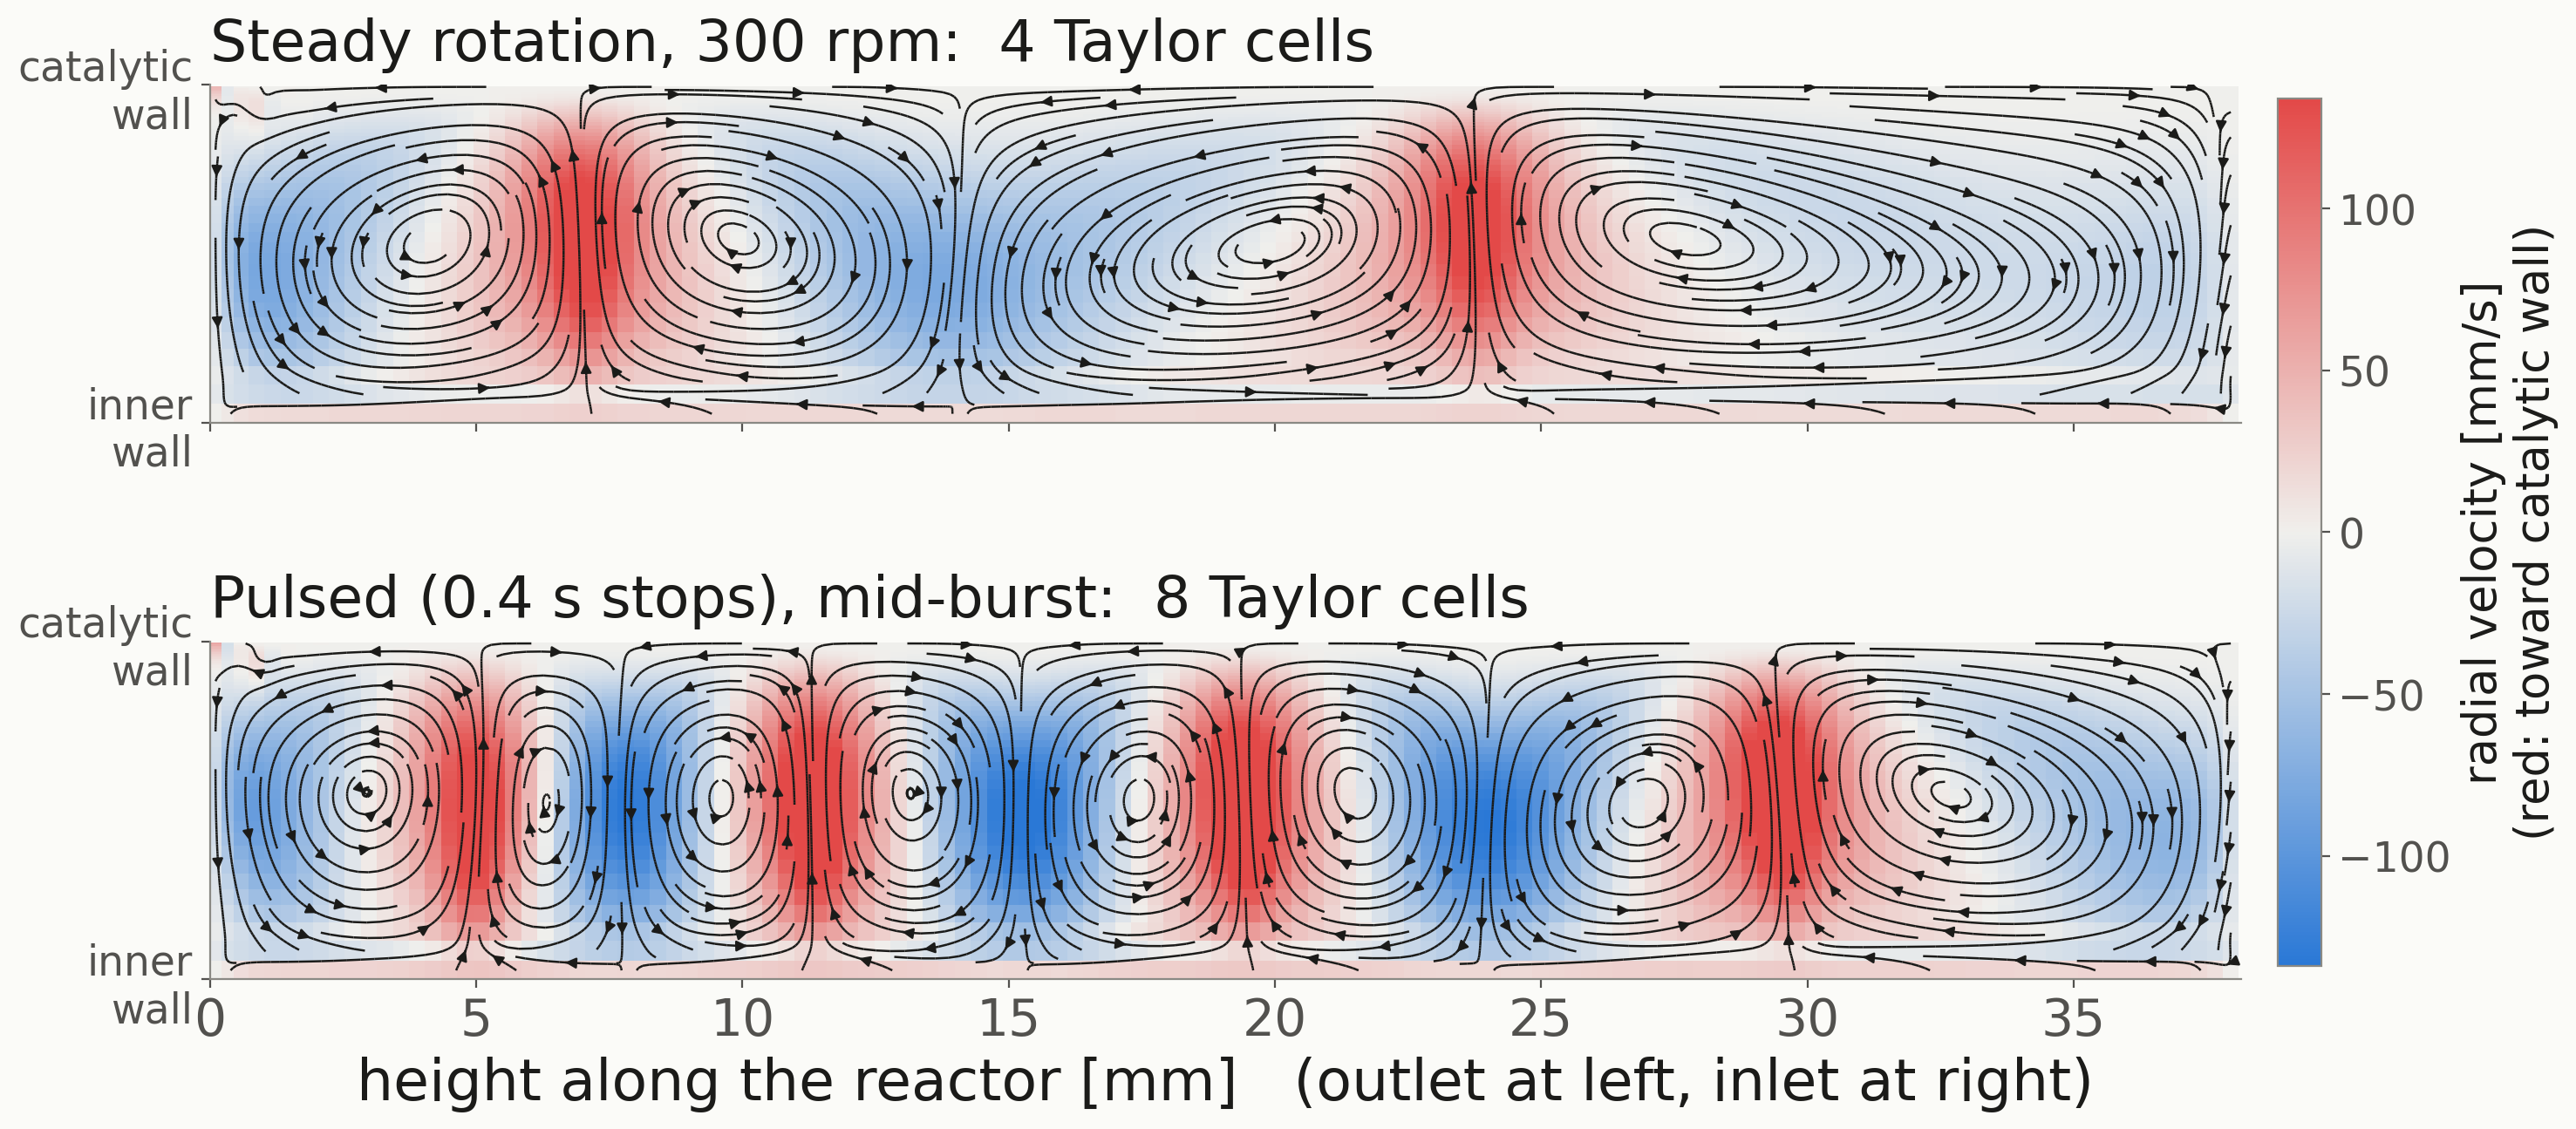
\includegraphics[width=\linewidth,height=0.86\textheight,keepaspectratio]{s_cells_snapshot}
\end{frame}
\note{[1:00] So why does a brief stop help? Both panels show the gap between the cylinders, unrolled sideways: inner wall at the bottom, catalytic wall at the top. Colour is radial velocity; red means liquid heading toward the catalytic wall. Under steady rotation there are four large vortex cells. Under pulsing, mid-burst, there are eight narrower ones. In dynamical-systems language this is multistability: at the same Reynolds number a short Taylor--Couette annulus has several stable solutions with different numbers of cells, and which one you land in depends on the initial condition; Benjamin and Mullin studied this in the early 1980s (check citation). Each brief stop brings the flow nearly to rest, and the restart from rest selects a higher axial wavenumber, eight cells instead of four. Narrower cells carry reactant to the wall faster.}

% ============================================================================
\begin{frame}{Restarts make the extra cells; steady rotation erases them}
  \begin{columns}[T]
    \begin{column}{0.49\textwidth}
      \centering{\small\textbf{Each cycle:} 8 cells, +15\% wall reaction}\par\smallskip
      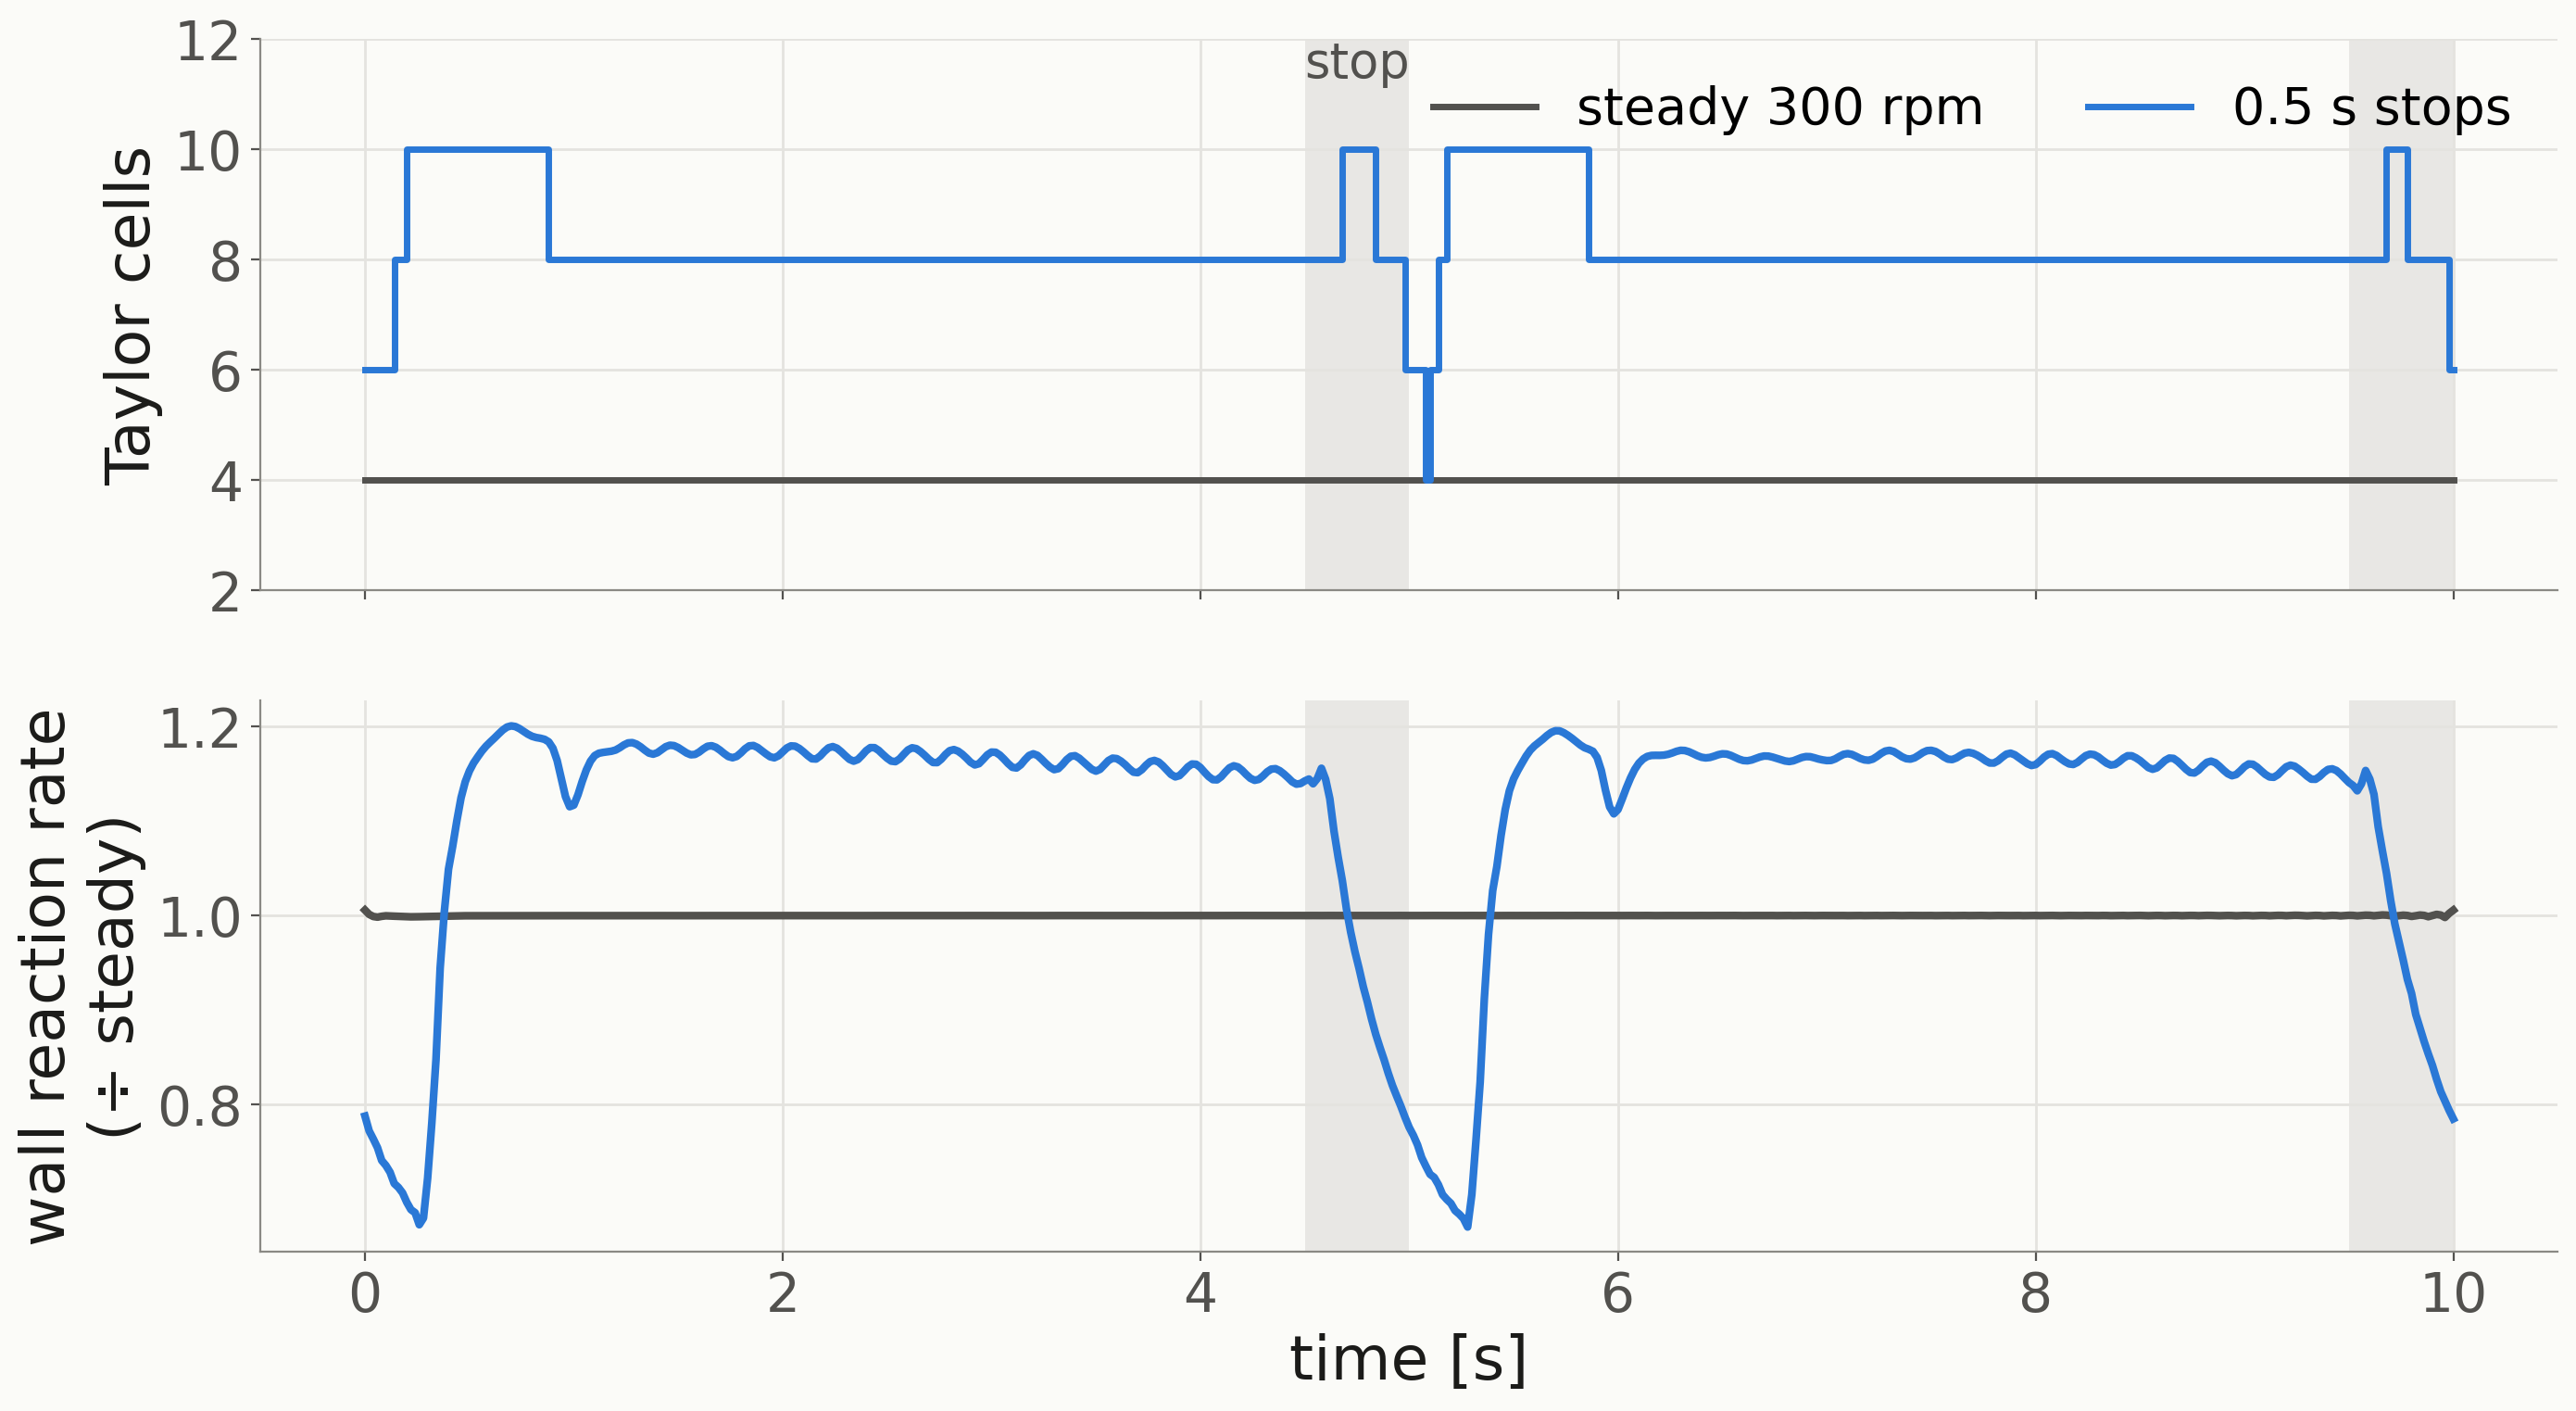
\includegraphics[width=\linewidth,height=0.56\textheight,keepaspectratio]{s_one_cycle}
    \end{column}
    \begin{column}{0.49\textwidth}
      \centering{\small\textbf{Stop pulsing:} back to 4 cells in 10--15\,s}\par\smallskip
      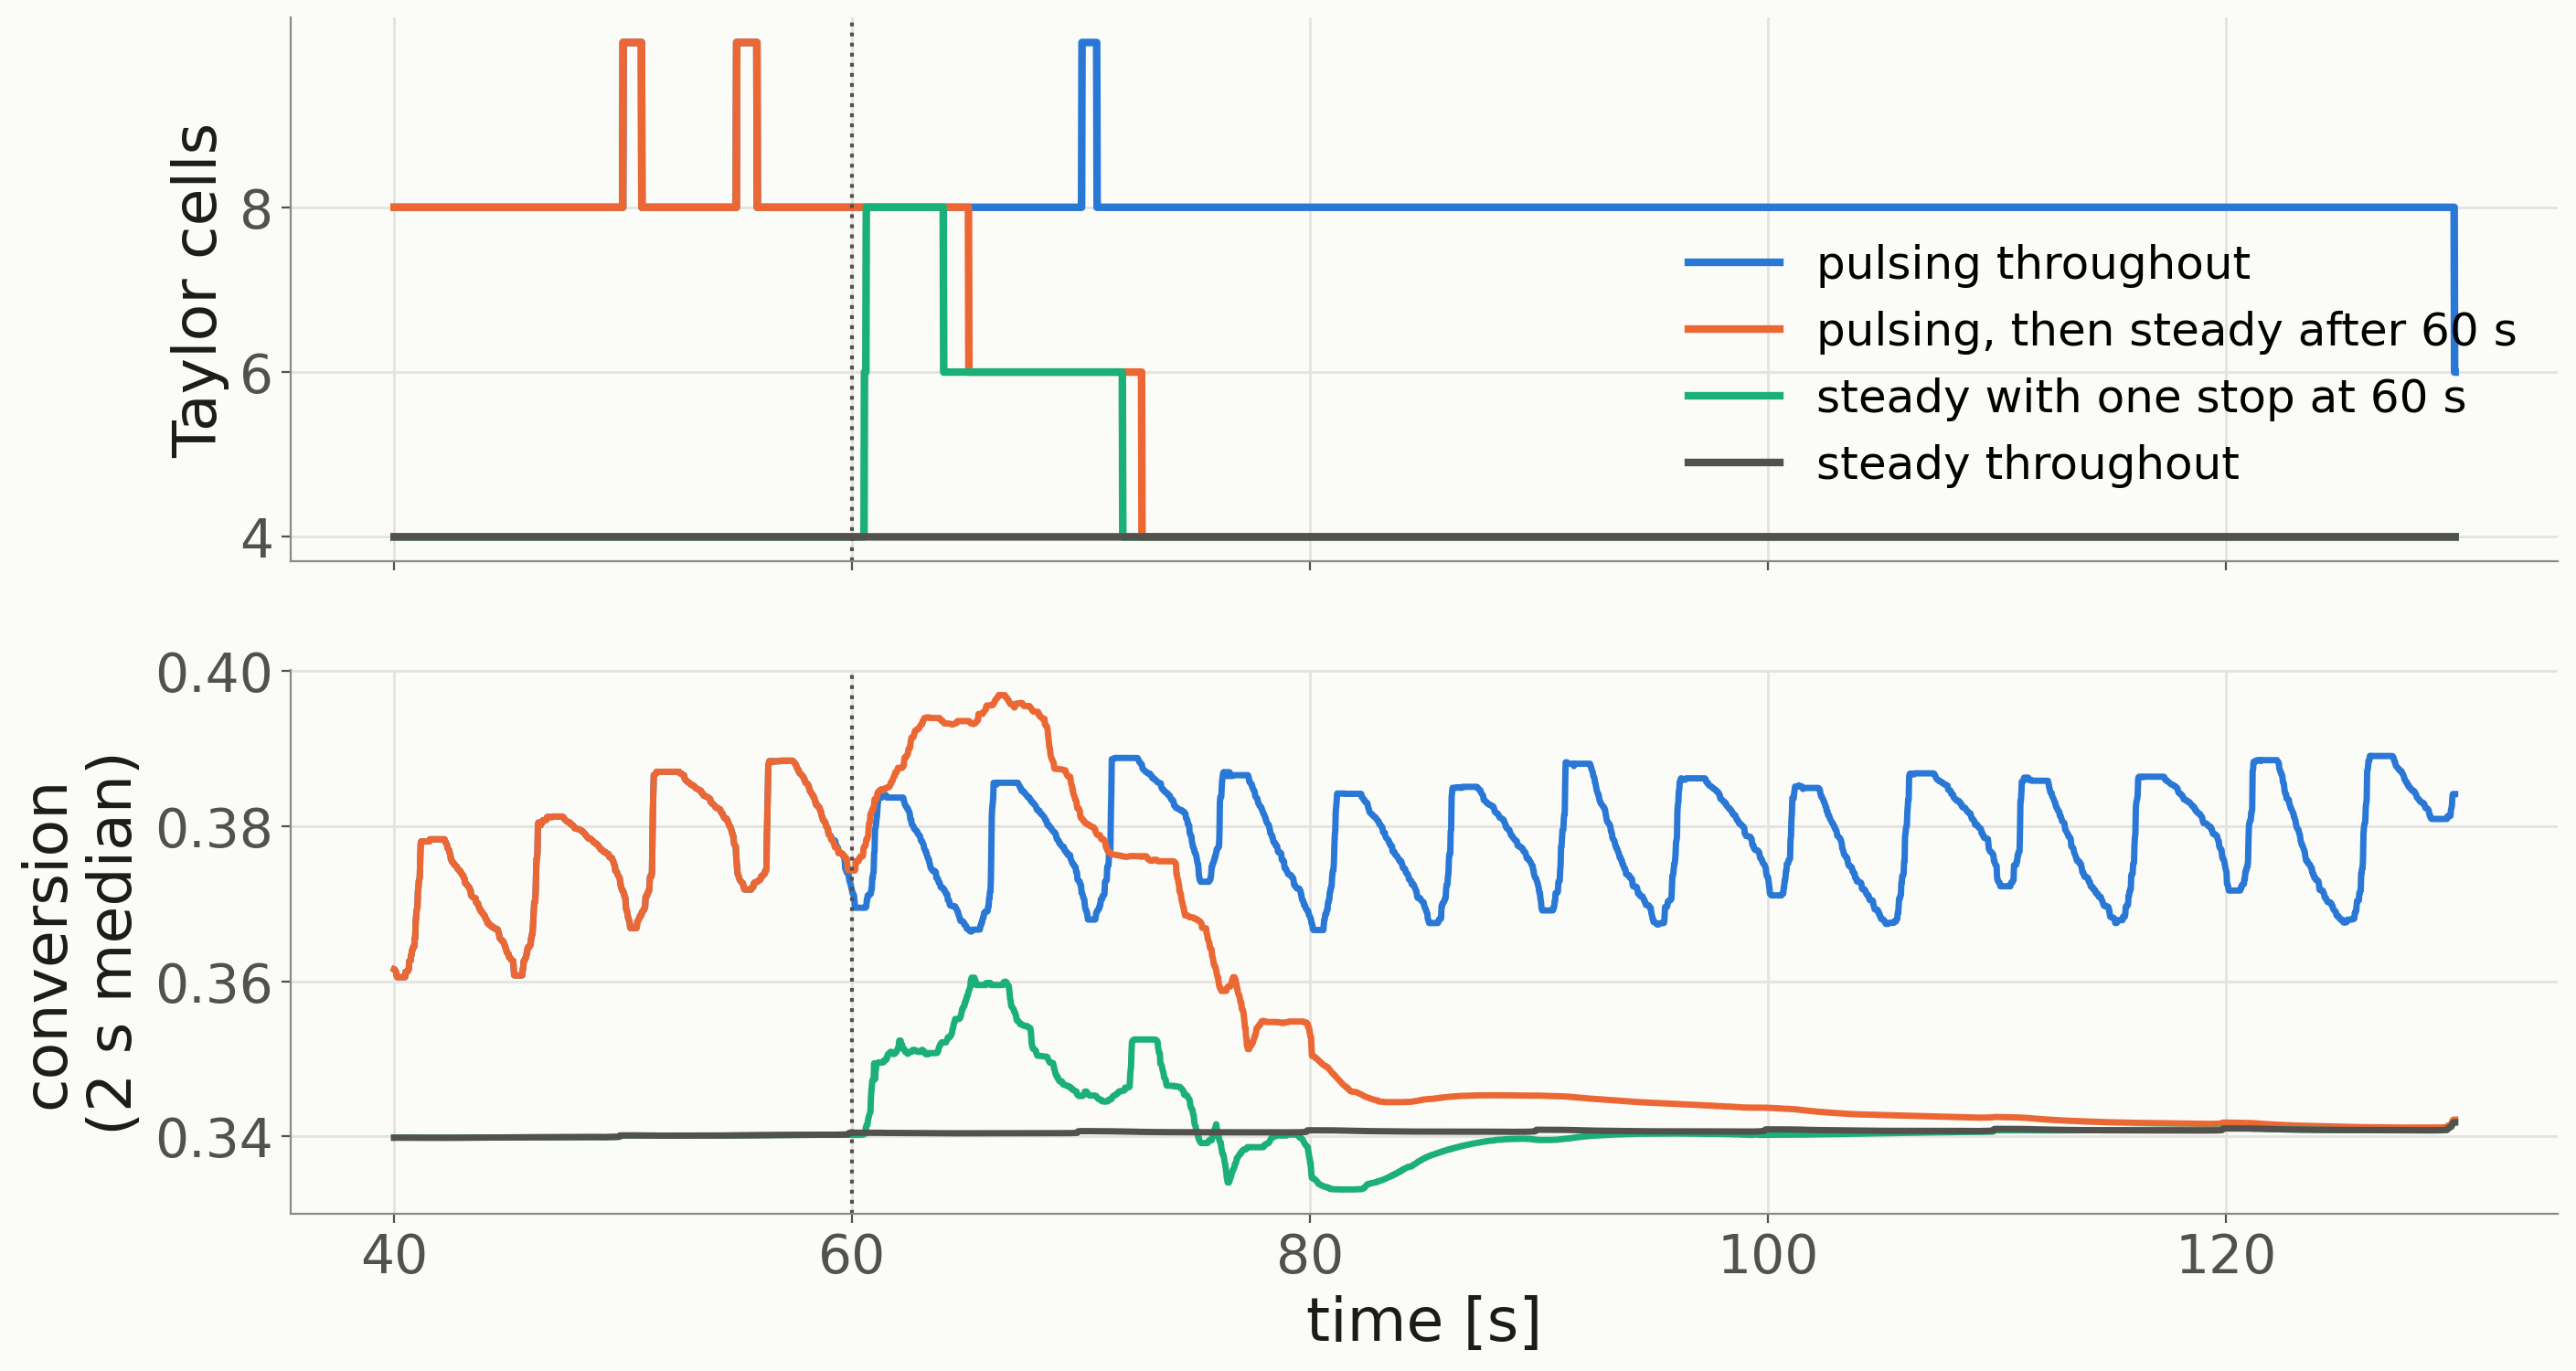
\includegraphics[width=\linewidth,height=0.56\textheight,keepaspectratio]{s_hold_kick}
    \end{column}
  \end{columns}
  \medskip
  \centering\alert{\textbf{Stops must repeat.}}
\end{frame}
\note{[1:00] Inside each cycle: after every restart the cell count jumps up and settles at eight, and the reaction rate at the wall stays about fifteen percent above steady rotation for the whole burst. It isn't a brief spike after the restart; the restart spike contributes almost nothing. On the right: if I pulse until 60 seconds and then hold steady, or do just one stop, the extra cells merge back to four within ten to fifteen seconds, and conversion drops back to the steady value. So the stops have to keep coming every few seconds, which explains why five-second cycles win and the published thirty-second cycle loses.}

% ============================================================================
\begin{frame}{It has to be a full stop}
  \begin{columns}[c]
    \begin{column}{0.68\textwidth}
      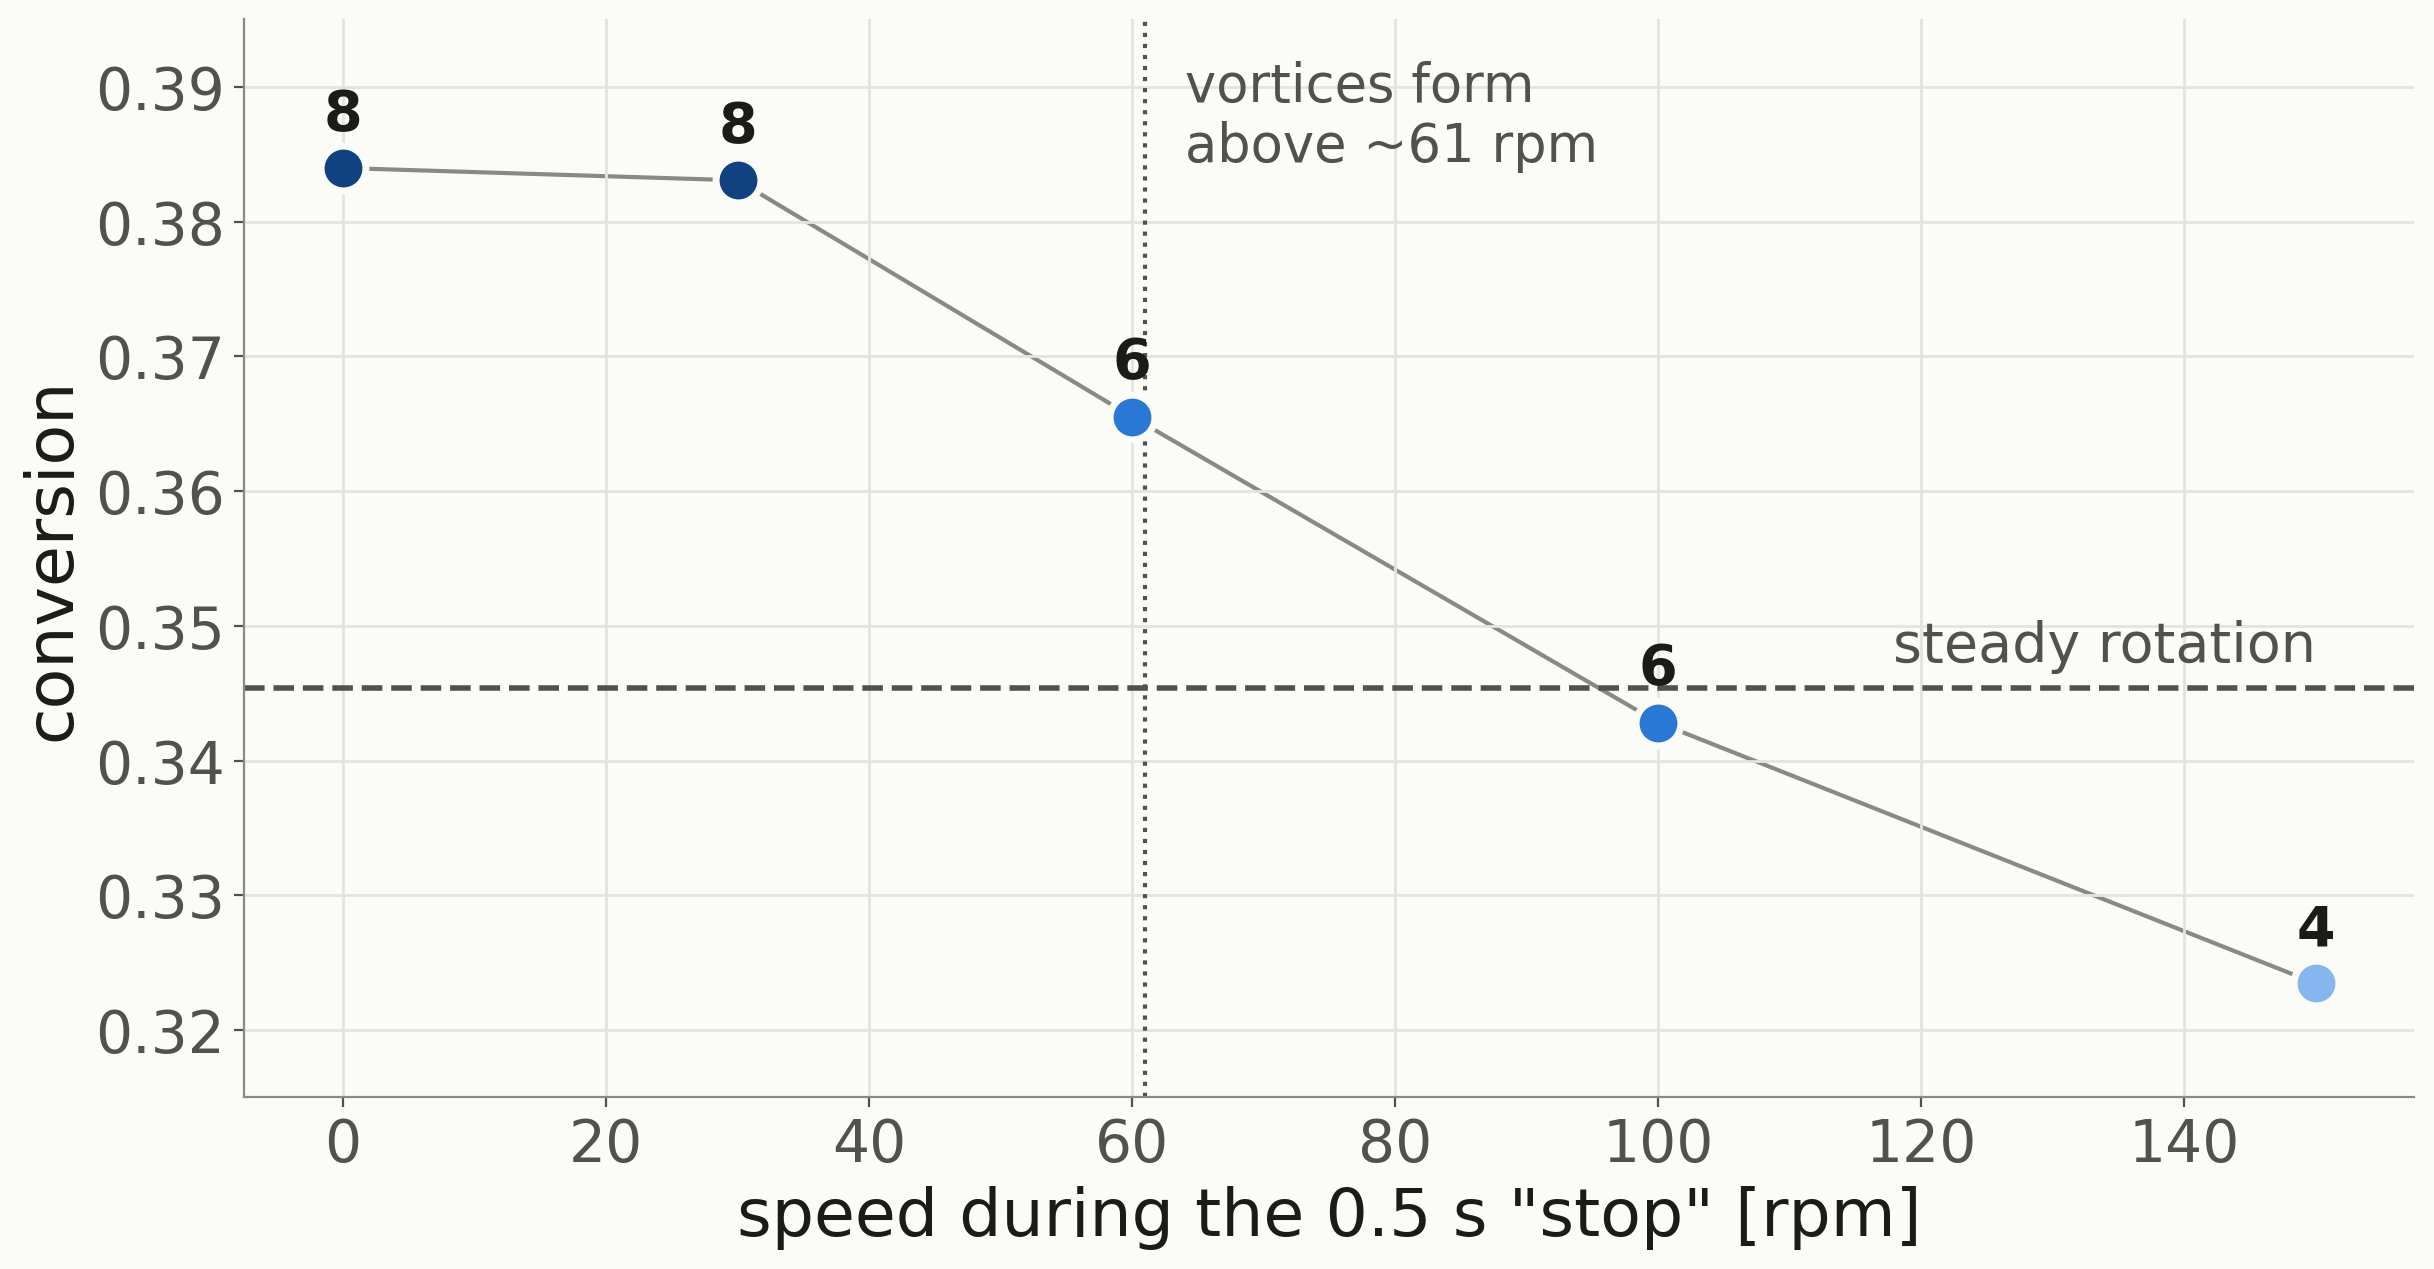
\includegraphics[width=\linewidth,height=0.76\textheight,keepaspectratio]{s_stop_level}
    \end{column}
    \begin{column}{0.30\textwidth}
      Vortices must die first.
    \end{column}
  \end{columns}
\end{frame}
\note{[0:30] Instead of stopping, I slowed the cylinder to 30, 60, 100 or 150 rpm for the same half second. Thirty is as good as a full stop. At 60 rpm, about where vortices start to form, you get six cells instead of eight, and at 100 and above the gain is gone. The vortices really have to die, to about one percent of their energy, before the restart can build a new, finer pattern.}

% ============================================================================
\begin{frame}{Conversion follows the cell count}
  \begin{columns}[c]
    \begin{column}{0.74\textwidth}
      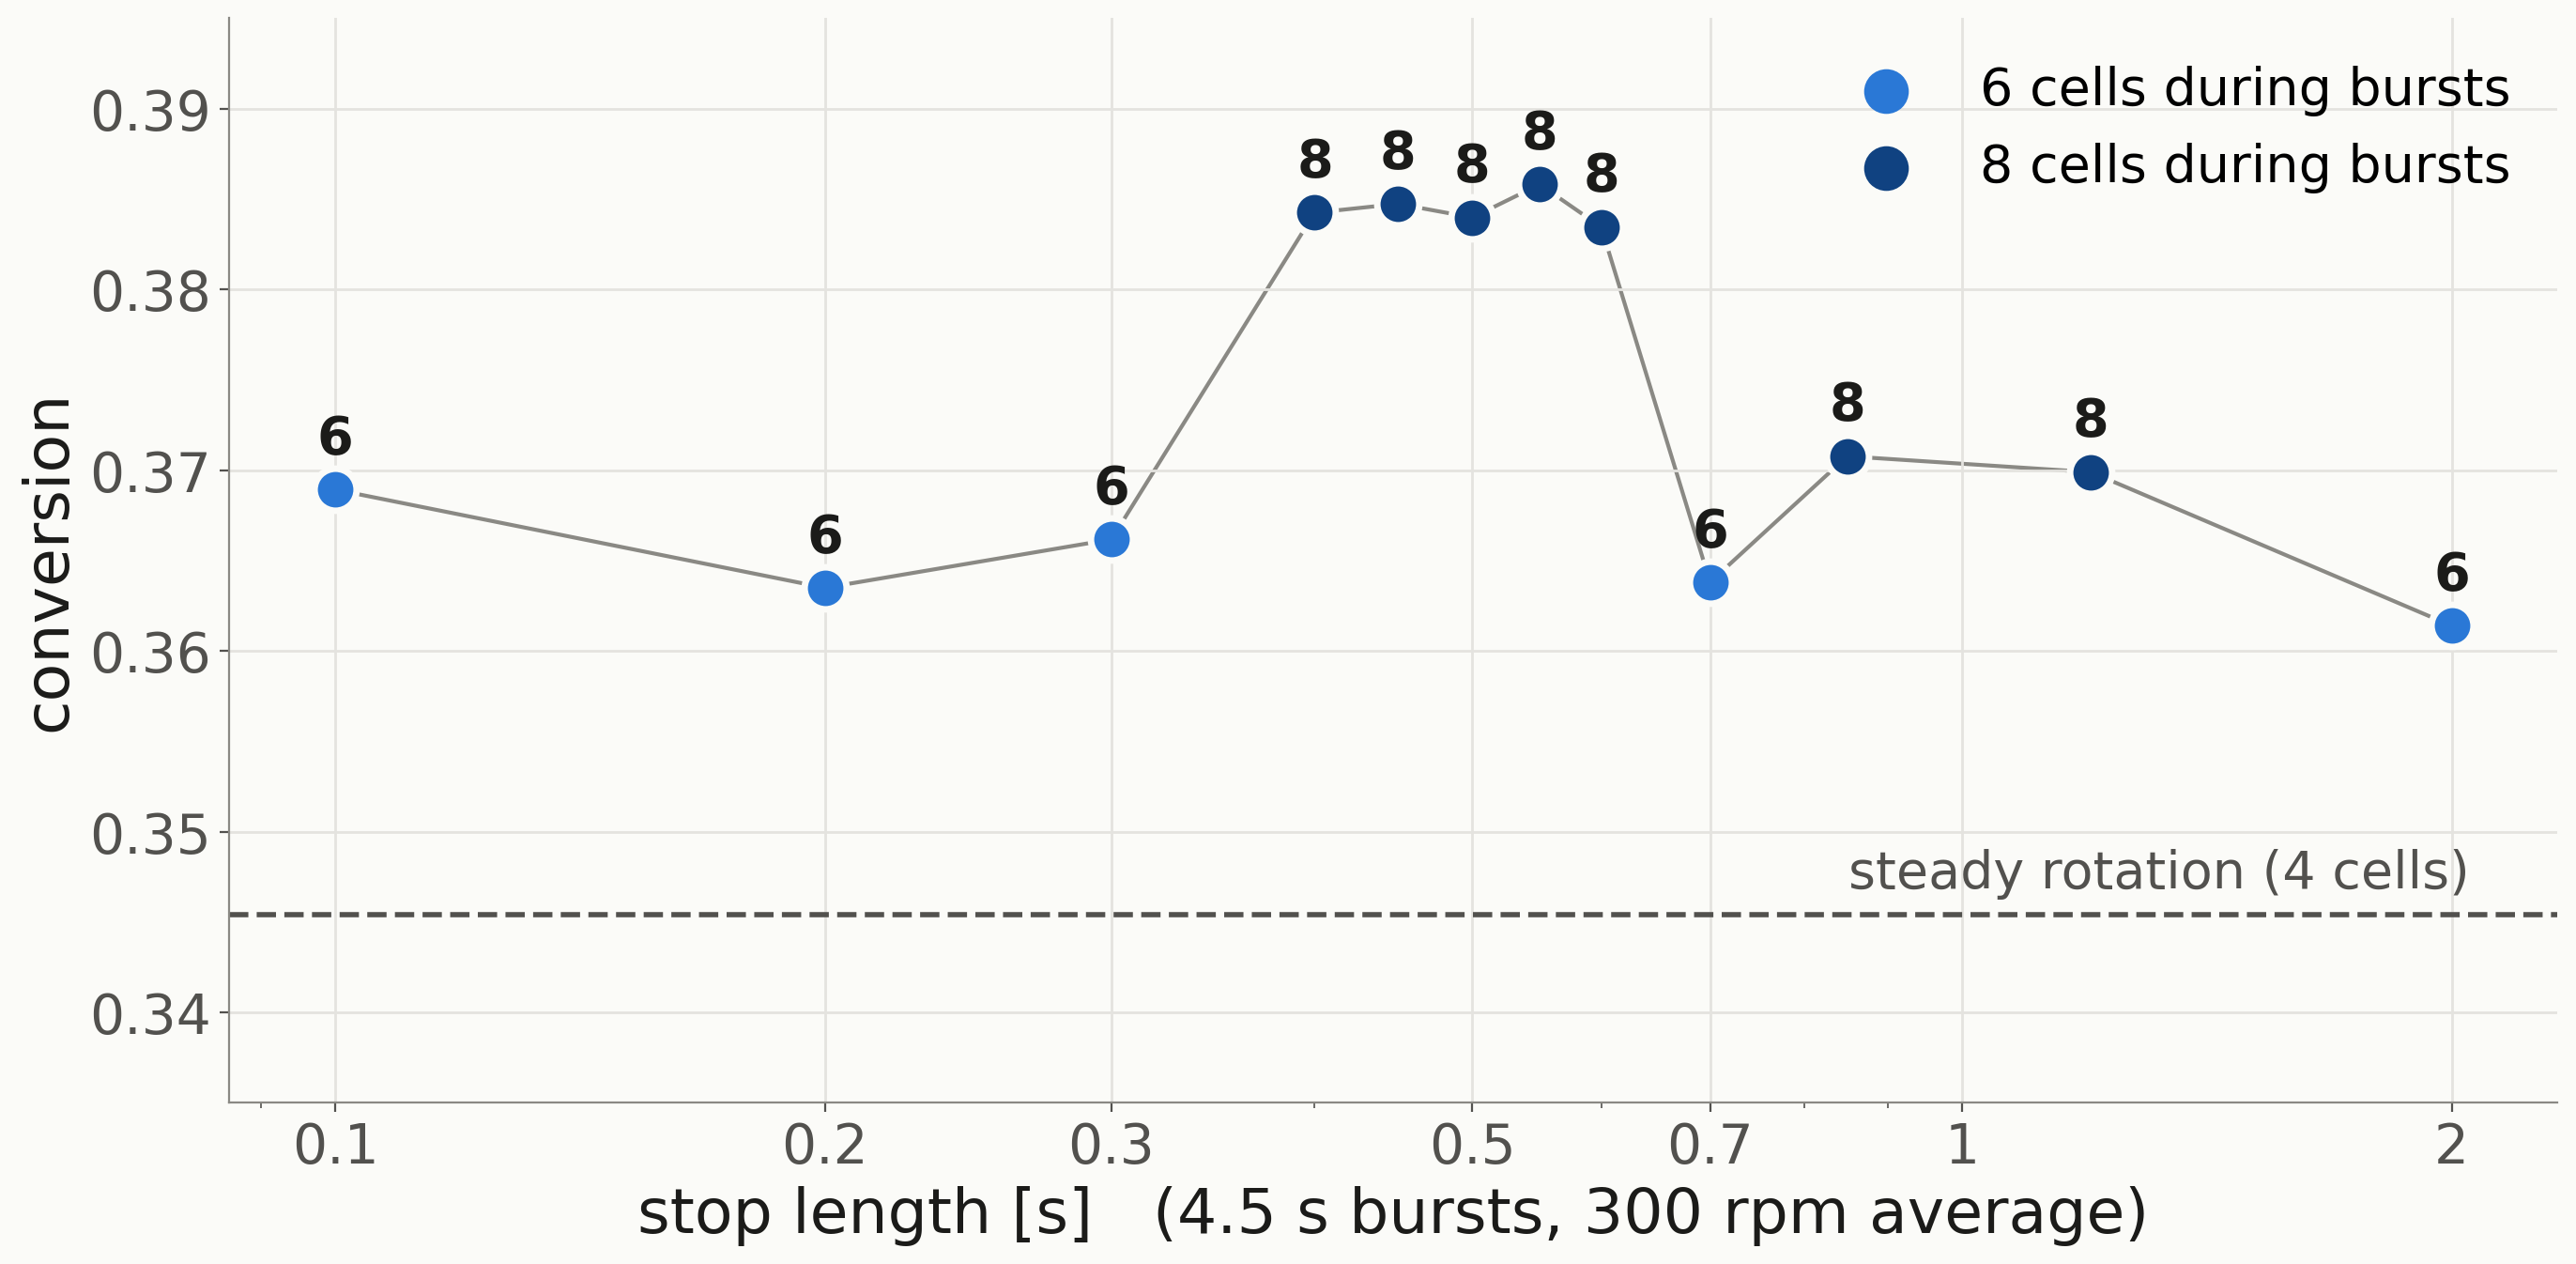
\includegraphics[width=\linewidth,height=0.74\textheight,keepaspectratio]{s_stop_curve_cells}
    \end{column}
    \begin{column}{0.24\textwidth}
      \bignum{+0.04}{conversion in the 8-cell window (0.4--0.6\,s stops)}\par\bigskip
      \bignum{4\,$\to$\,8}{cells, steady vs best pulsing}
    \end{column}
  \end{columns}
\end{frame}
\note{[0:45] Plot conversion against stop length and label each point with its cell count. It isn't a smooth curve with one peak; it's a set of levels. Steady rotation, four cells, at the bottom; six-cell stops in the middle; and the best stops, 0.4 to 0.6 seconds, are exactly the ones whose restart lands in eight cells, about 0.04 above steady rotation. The sudden drop at 0.7 seconds, which looked like a strange cliff in the original search, is just the flow falling back to six cells.}

% ============================================================================
\begin{frame}{Numerical verification}
  \begin{columns}[T]
    \begin{column}{0.58\textwidth}
      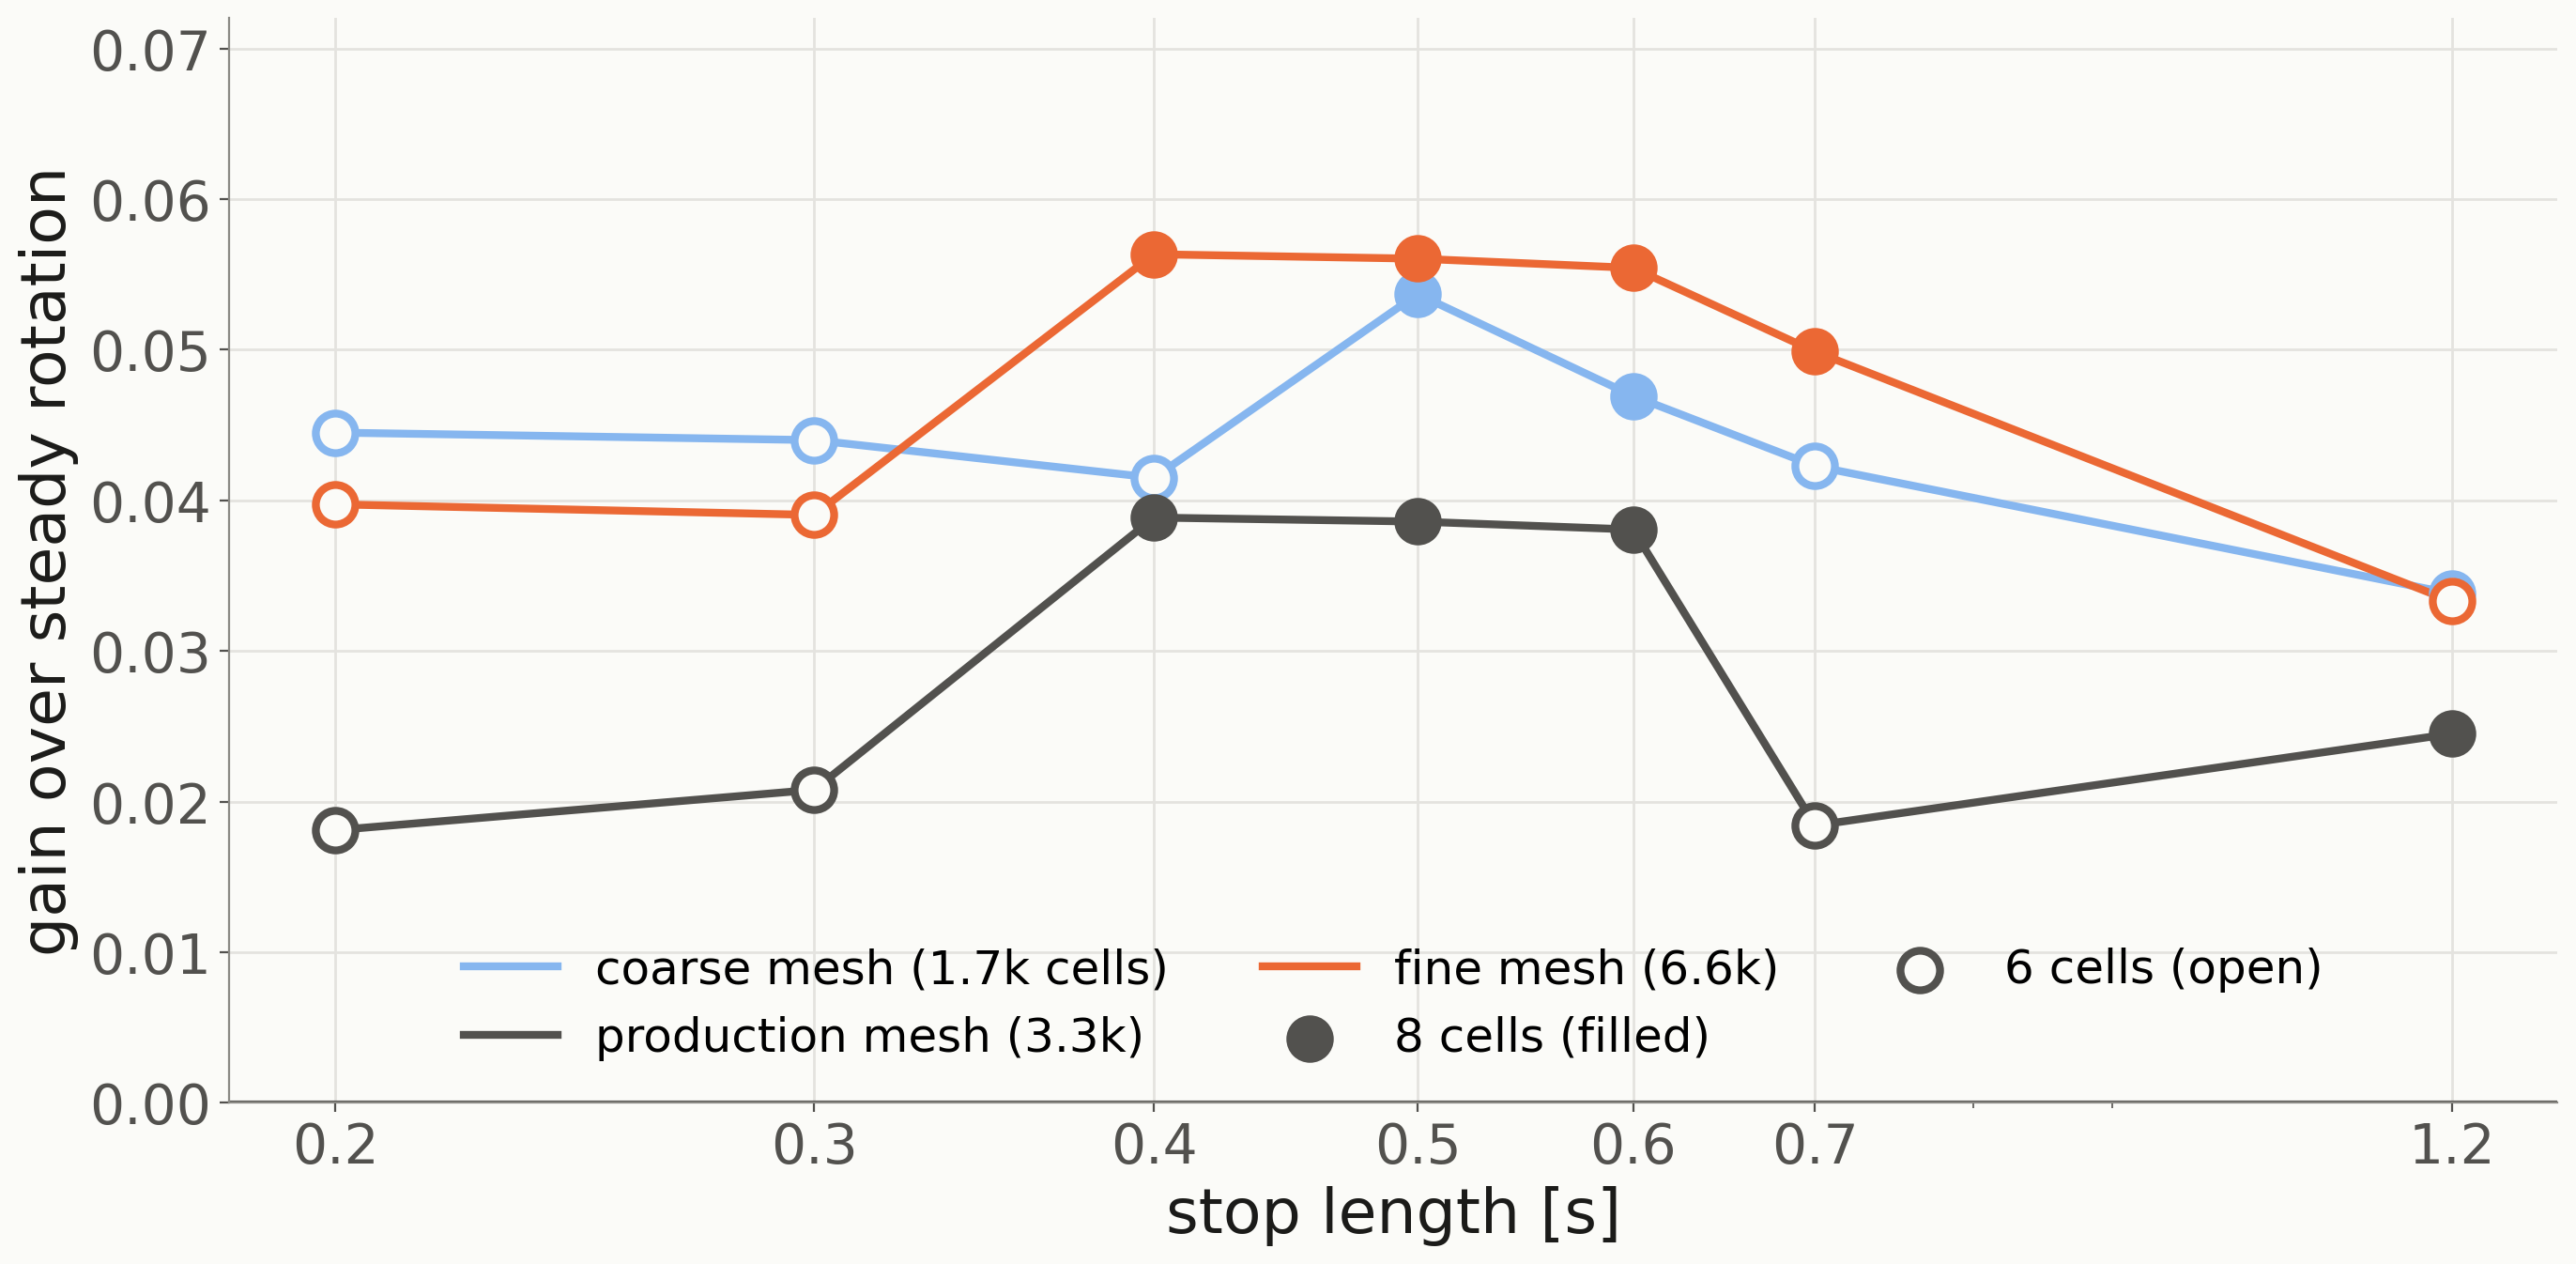
\includegraphics[width=\linewidth,height=0.62\textheight,keepaspectratio]{s_mesh_check}\par
      {\small\color{ink}3 meshes: same cells, gain +0.04 to +0.06}
    \end{column}
    \begin{column}{0.40\textwidth}
      \begin{block}{Checks}
        \begin{itemize}
          \item Half time step: outlet artifact gone
          \item Mass balance: 0.3\%
          \item Replicate noise: 0.002
        \end{itemize}
      \end{block}
    \end{column}
  \end{columns}
\end{frame}
\note{[0:45] For this audience the obvious question is whether it's numerics. I repeated the key runs on a coarser and a finer mesh from the same self-similar family. On all three, steady rotation has four cells, the best stops land in eight, and the gain is four to six hundredths. Halving the time step exposed and removed a spurious jet at the outlet worth about four hundredths of conversion, which is why all these runs use the smaller step. The mass balance closes to a third of a percent and replicate noise is about 0.002. What does move with the mesh is the exact edges of the eight-cell window, by a tenth of a second or two, so I quote ``about half a second''.}

% ============================================================================
\begin{frame}{Three takeaways}
  \begin{enumerate}
    \setlength\itemsep{0.8em}
    \item Brief full stops beat steady rotation and the published recipe.
    \item RL learns near-optimal control: matches 220-run optimization, transfers $5\times$ taller.
    \item Mechanism: restarts select more Taylor cells (8 vs 4); stops must repeat.
  \end{enumerate}
  \vfill
  {\small\color{ink}\textbf{Next:} messy conditions (feed, fluid drift) $\to$ feedback control; 3D check.\par\smallskip
  \textbf{Limits:} 2D axisymmetric; $\mathrm{Sc}=1075$.}
\end{frame}
\note{[0:45] One: brief full stops beat steady rotation at the same power, and beat the published recipe. Two: the RL pipeline learns near-optimal control from simulation alone. With no physics given, it matched an independent 220-run optimization, which is how we know it found the right answer, and it carried over to a reactor five times taller. Three: the optimum exploits multistability. Each restart selects a state with more cells that transports reactant faster, and because that state decays back under steady forcing, the stops have to repeat. This problem turned out to be simple: steady conditions, one best waveform, so a static optimizer can solve it too, and RL tying it is what you'd expect. The next step is to make it messy: changing feed rates and drifting fluid properties, where no fixed waveform stays right and a feedback policy should pull ahead. The main limit is the 2D model, so the mechanism is still a hypothesis for real 3D flow. Thank you, happy to take questions.}

% ============================================================================
\appendix
\begin{frame}{Backup: best fixed waveform vs the RL policy}
  \centering
  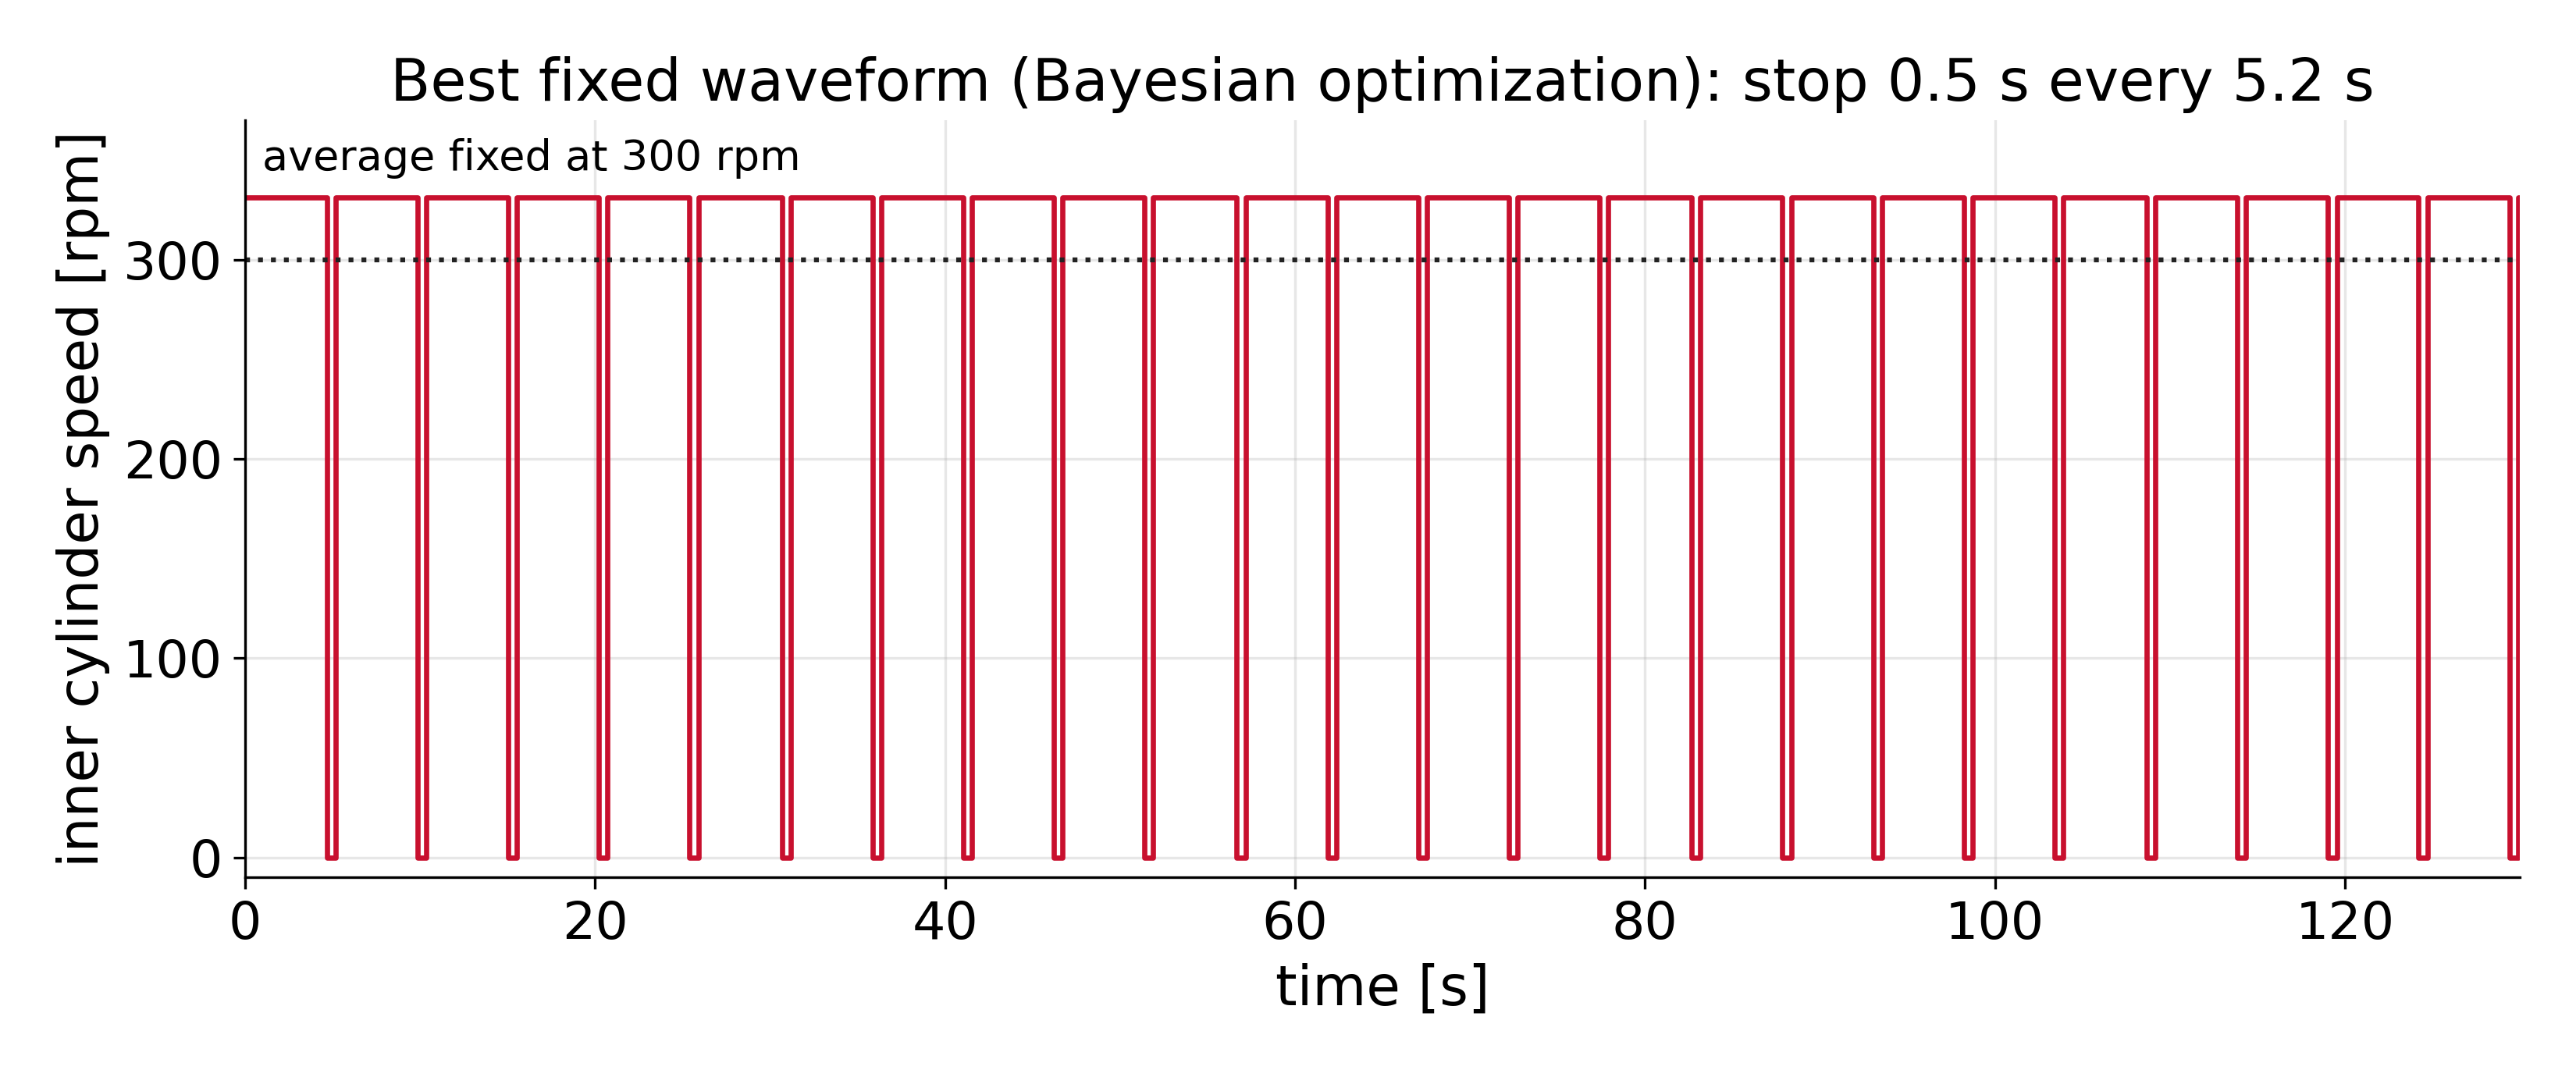
\includegraphics[width=0.86\linewidth,height=0.40\textheight,keepaspectratio]{bo_best_waveform}\par\smallskip
  \includegraphics[width=0.86\linewidth,height=0.40\textheight,keepaspectratio]{fig4_learned_waveform}
\end{frame}
\note{[Backup] Top: the best fixed waveform from the 220-run Bayesian optimization, stop half a second every five seconds, peak about 330 rpm. Bottom: what the RL policy chose. Same idea, brief full stops at high duty, but RL's stops are shorter, mostly a tenth to four tenths of a second, which mostly lands in the six-cell state and costs it one to two hundredths of conversion.}

% ============================================================================
\begin{frame}{Backup: why 0.5\,s? Two time scales, two predictions}
  \begin{columns}[T]
    \begin{column}{0.48\textwidth}
      \begin{block}{Swirl decay}
        \[ \tau = \frac{d^2}{\pi^2 \nu} \approx 0.4\ \mathrm{s} \]
        Slowest decay mode of momentum diffusion across the gap. Predicts best stop $\propto \nu^{-1}$.
      \end{block}
    \end{column}
    \begin{column}{0.48\textwidth}
      \begin{block}{Wall layer}
        \[ \tau = \frac{\delta^2}{D} \approx 0.8\ \mathrm{s} \]
        Regrowth of the depleted layer at the wall. At fixed $D$, predicts best stop $\propto \nu^{0.3}$ to $\nu^{0.7}$.
      \end{block}
    \end{column}
  \end{columns}
  \bigskip
  \takeaway{\textbf{Test:} vary $\nu$ at fixed $D$ and fit best stop $\propto \nu^{a}$. The sign of $a$ decides.}
\end{frame}
\note{[Backup] If asked whether a simple time scale explains the stop length: why half a second? Two time scales sit near it. One is the decay of the swirl: the slowest mode of momentum diffusion across a gap of width d decays on d squared over pi squared nu, about 0.4 seconds. The other is the time for the reactant-depleted layer at the wall to regrow, delta squared over D, about 0.8 seconds. They scale differently with viscosity. Holding the diffusivity fixed, the swirl clock predicts the best stop goes like nu to the minus one; the wall-layer clock predicts a positive power, about 0.3 to 0.7. So I varied the viscosity, fit an exponent, and decided in advance that its sign would pick the winner.}

% ============================================================================
\begin{frame}{Backup: neither guess sets the best stop}
  The swirl decays exactly as theory says (left), but the best stop follows neither prediction (right).\par\medskip
  \centering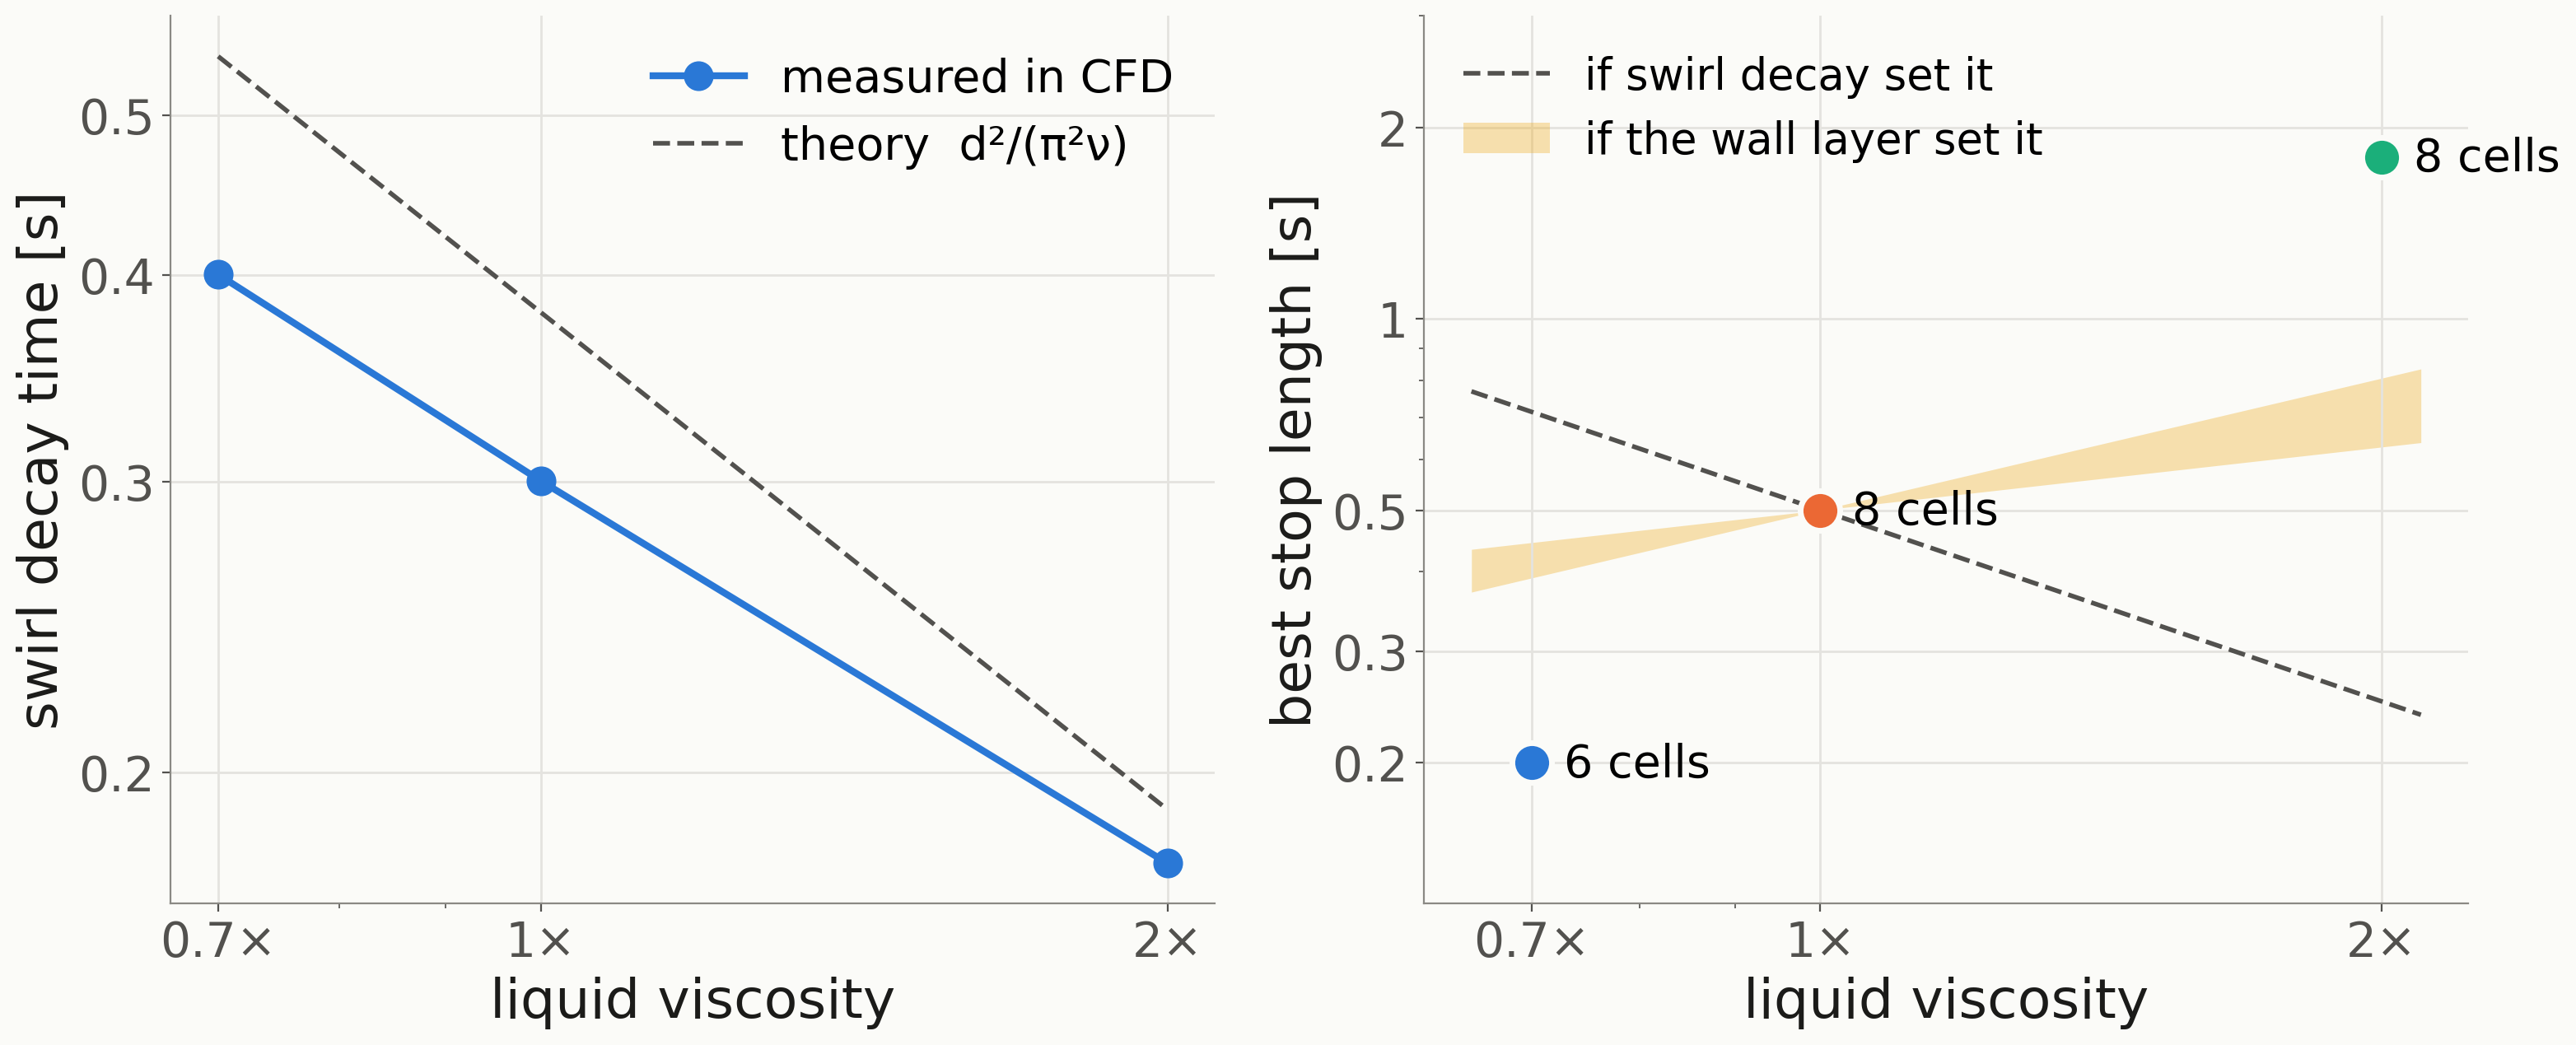
\includegraphics[width=\linewidth,height=0.66\textheight,keepaspectratio]{s_clocks}
\end{frame}
\note{[Backup] On the left, the swirl decays exactly as the eigenmode estimate says, one over viscosity. On the right, the best stop follows neither prediction; a formal exponent fit isn't even meaningful, because the optimum jumps rather than drifting. The labels, six cells and eight cells, are the clue.}


\begin{frame}{Backup: the gain is a higher plateau, not a restart spike}
  \centering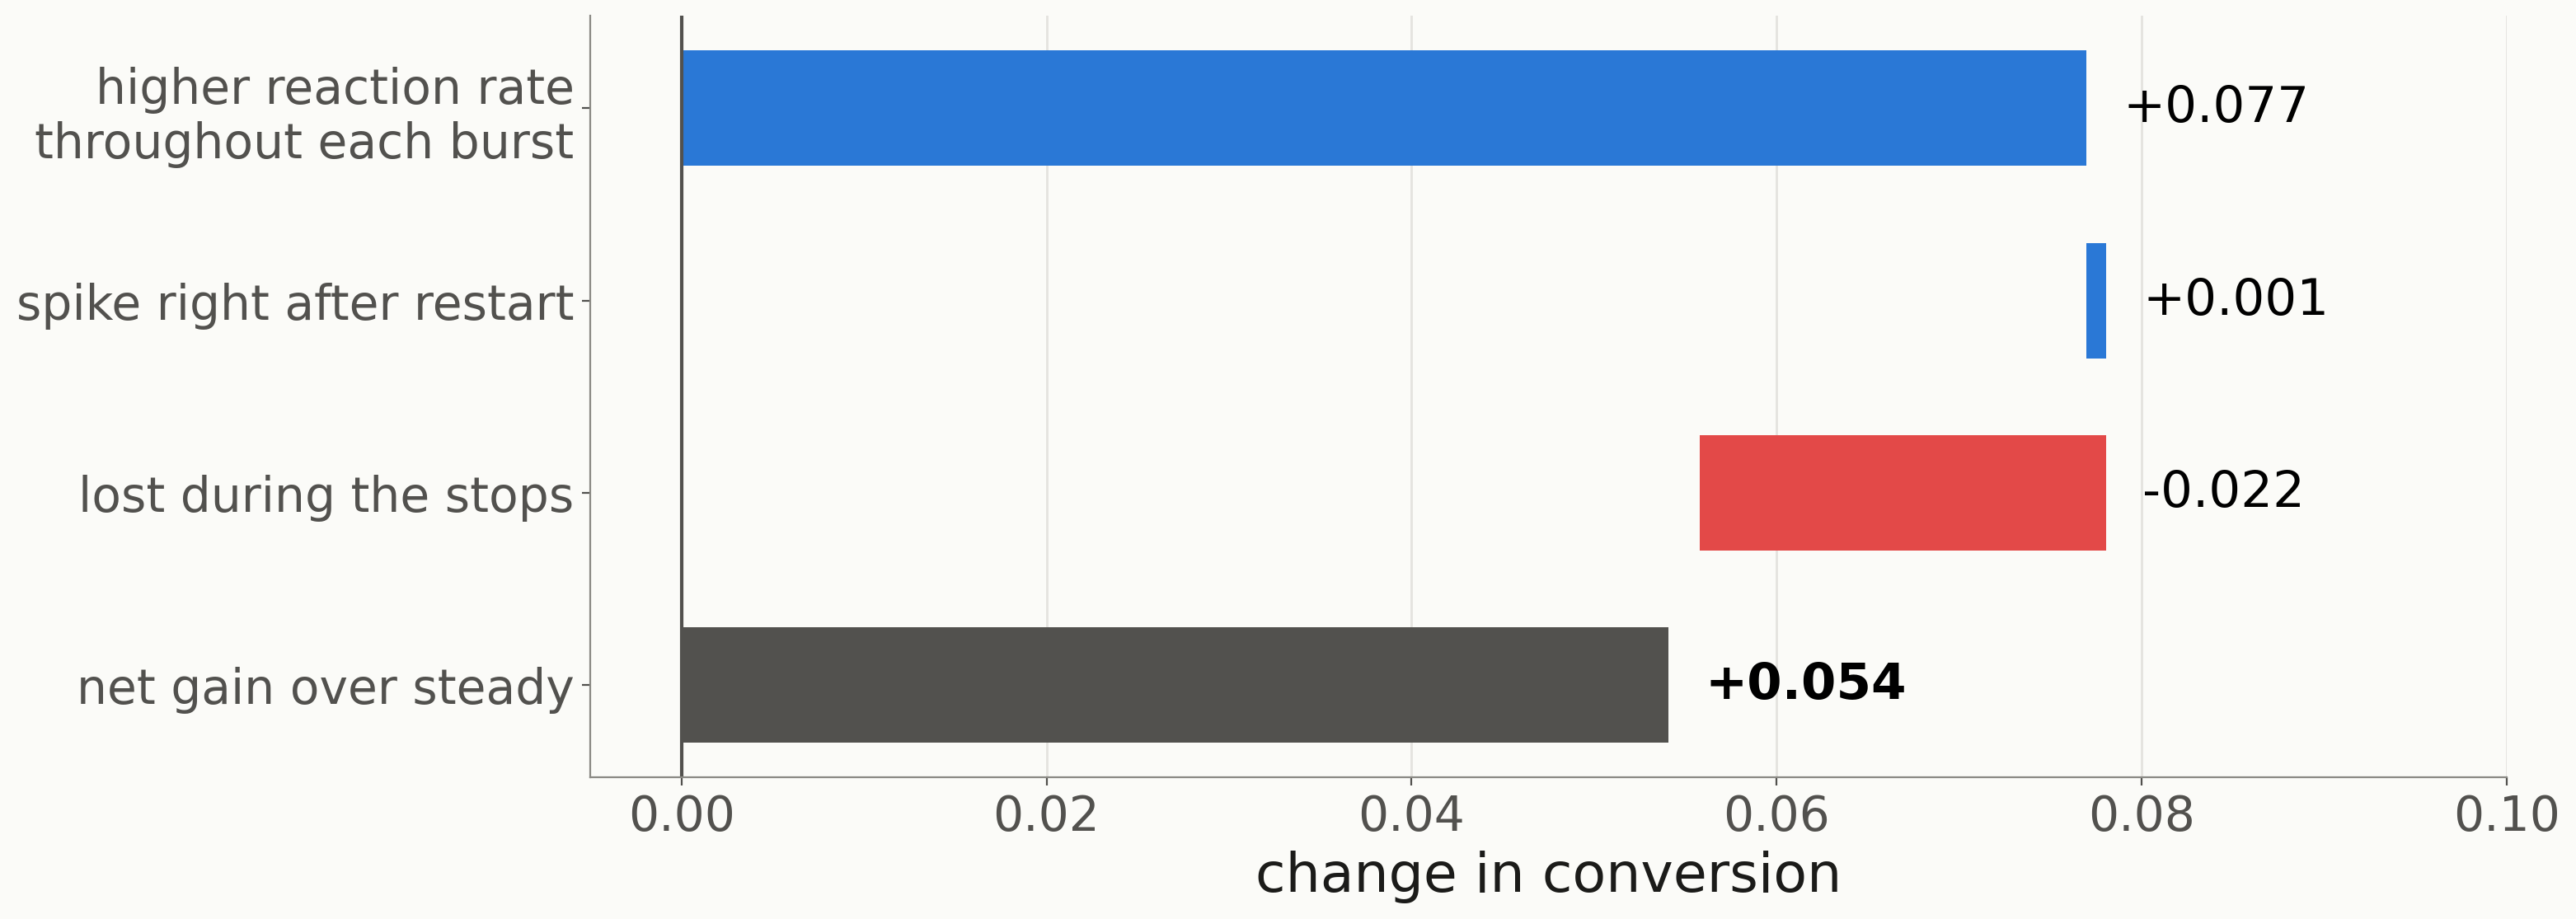
\includegraphics[width=\linewidth,height=0.62\textheight,keepaspectratio]{s_gain_breakdown}\par\smallskip
  \raggedright{\small\color{ink}From the wall-reaction traces of the best waveform's original run (wall-flux budget, last 26\,s).}
\end{frame}
\note{[Backup] If asked whether this is just a restart spike (``film renewal''): no. Splitting the gain over steady rotation: +0.077 from the reaction rate staying higher through the whole burst, only +0.001 from the spike right after restart, and $-0.022$ lost while stopped. The parts sum to 0.056 against the measured 0.054; the difference comes from how the burst plateau is defined.}

\begin{frame}{Backup: gain needs cells added over steady rotation}
  \begin{columns}[c]
    \begin{column}{0.64\textwidth}
      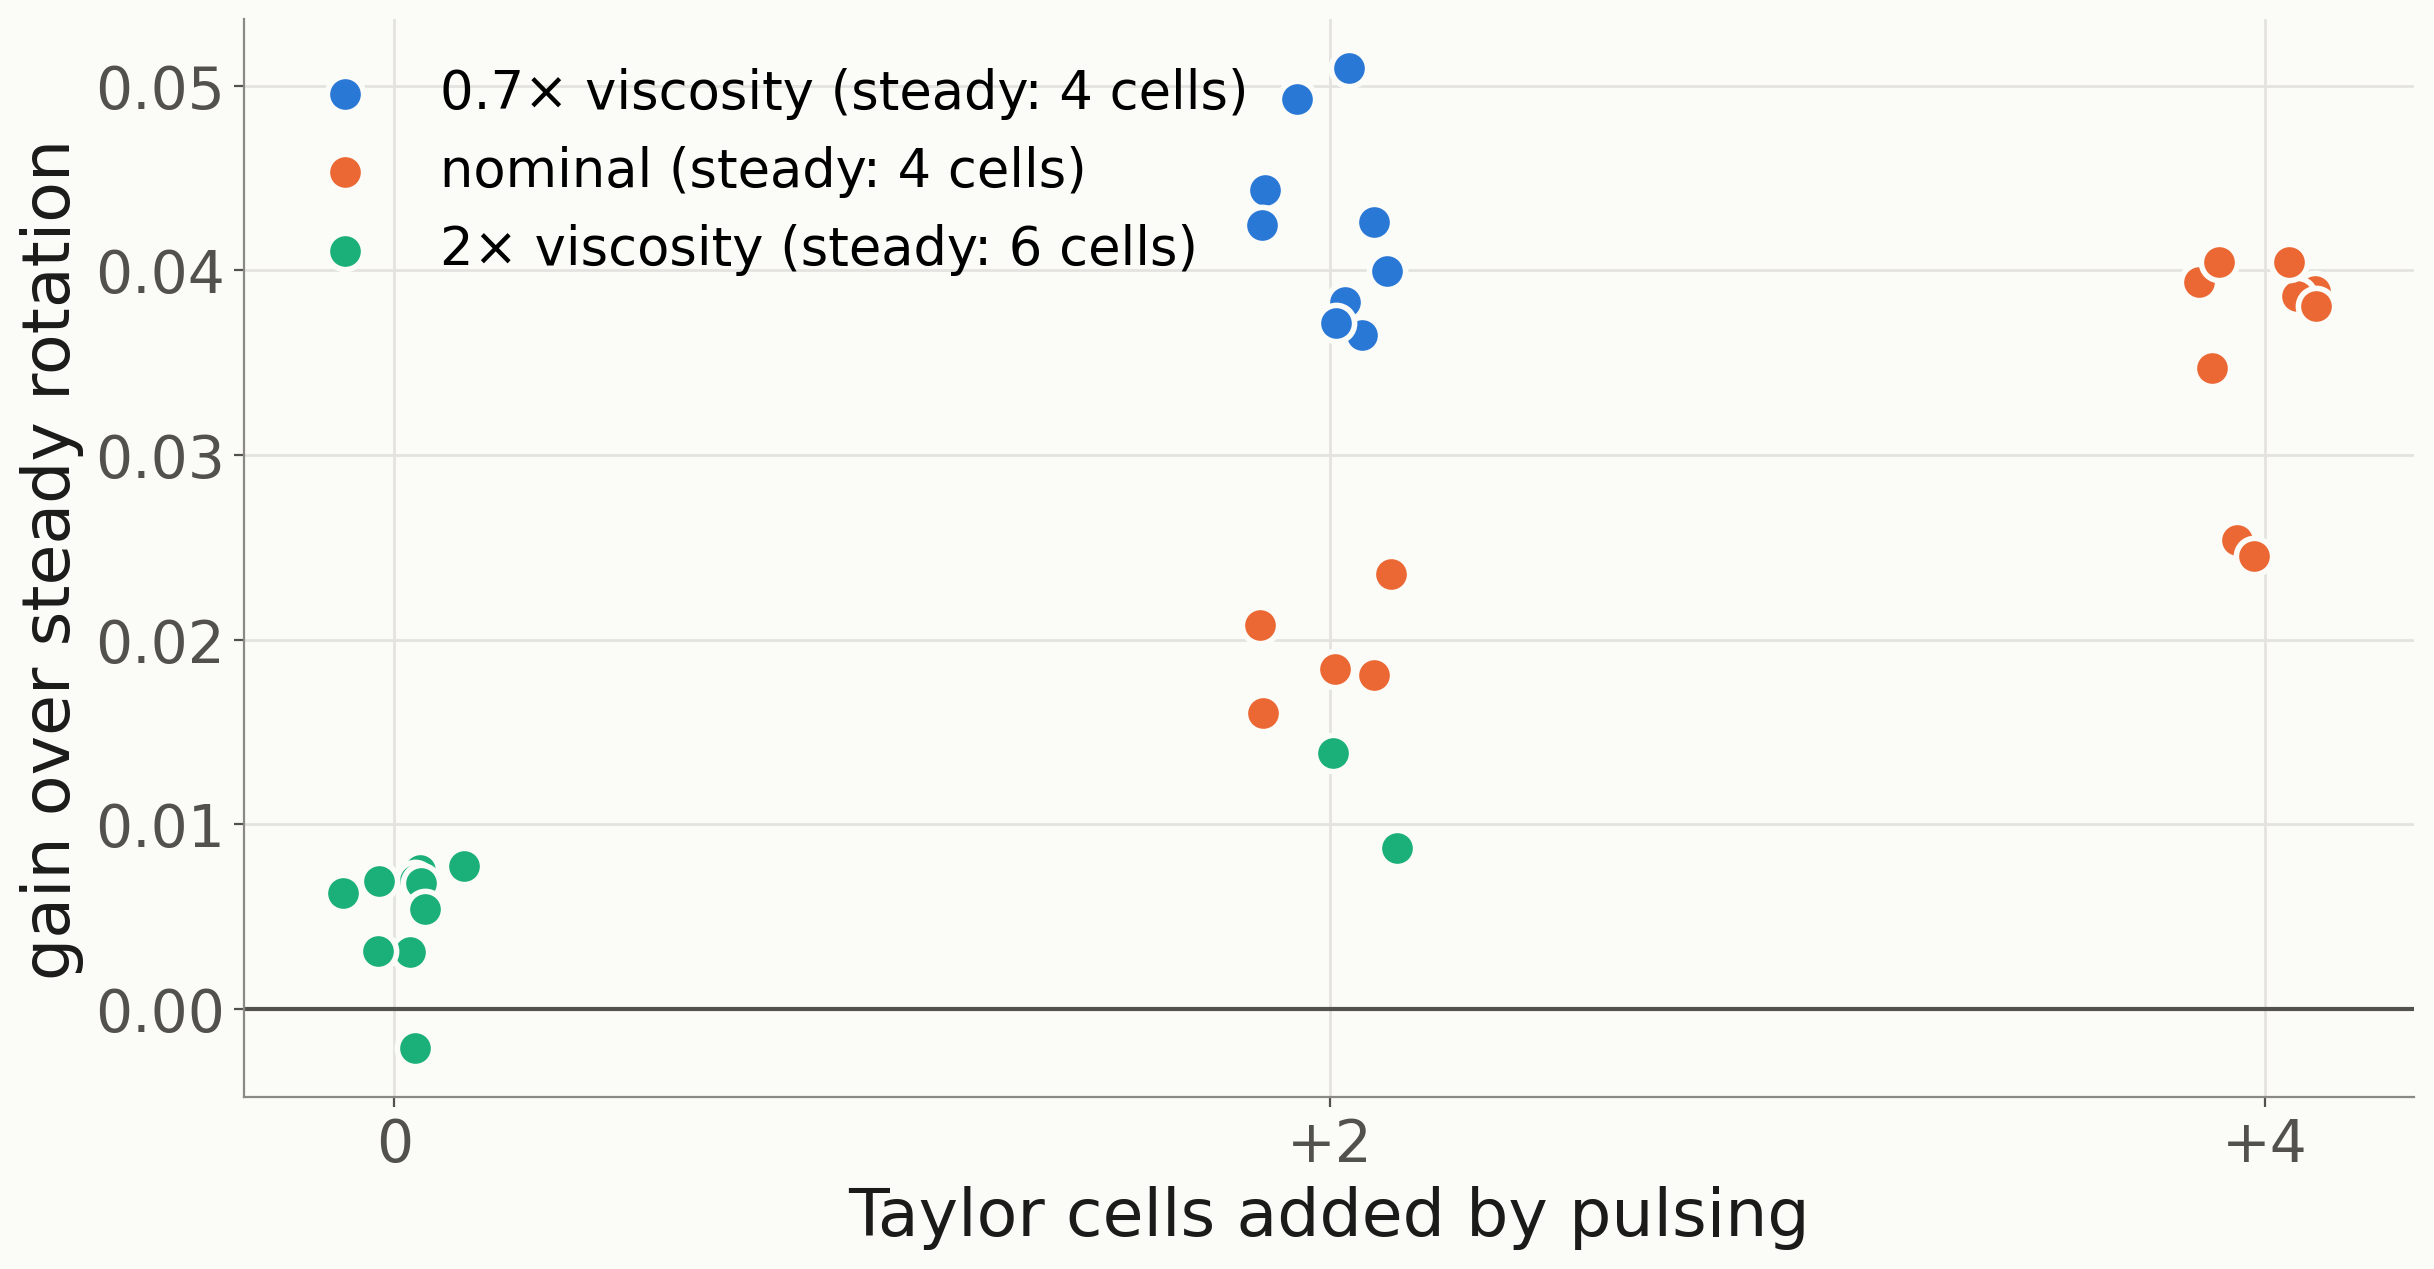
\includegraphics[width=\linewidth,height=0.72\textheight,keepaspectratio]{s_cells_added_gain}
    \end{column}
    \begin{column}{0.34\textwidth}
      At $2\times$ viscosity, steady rotation already holds 6 cells. Most pulses add none, and the gain shrinks to about +0.01.
    \end{column}
  \end{columns}
\end{frame}
\note{[Backup] Every pulsed run from the viscosity sweep, by how many cells pulsing adds over steady rotation at that viscosity. Runs that add no cells gain almost nothing; runs that add two or four gain up to five hundredths. At twice the viscosity steady rotation already has six cells, so most pulses add none. The size of the gain also depends on viscosity, so it isn't one universal curve.}

\begin{frame}{Backup: electrical power model}
  \begin{columns}[T]
    \begin{column}{0.58\textwidth}
      \begin{block}{L\'opez-Guajardo et al.\ (2024), \S3.4, Eqs.\ 18--23}
        {\small
        \[ T_{\mathrm{mot}} = \underbrace{J_{\mathrm{tot}}\,\dot\omega}_{\text{inertia}}
           + \underbrace{T_0\,\mathrm{sign}(\omega)}_{\text{bearings}}
           + \underbrace{\beta_2\,\omega^2\,\mathrm{sign}(\omega) + \beta_1\,\omega}_{\text{drag}} \]
        \[ i_{\mathrm{mot}} = \frac{T_{\mathrm{mot}}}{K_t}, \qquad
           e_{\mathrm{mot}} = L\,\frac{di_{\mathrm{mot}}}{dt} + R\,i_{\mathrm{mot}} + K_e\,\omega \]
        \[ P_{\mathrm{mot}} = e_{\mathrm{mot}}\, i_{\mathrm{mot}}, \qquad
           P_e = \begin{cases} P_{\mathrm{mot}}/\eta, & P_{\mathrm{mot}} \ge 0 \\ P_{\mathrm{mot}}\,\eta, & P_{\mathrm{mot}} < 0 \end{cases} \]}
      \end{block}
      {\small\color{ink}Evaluated on the commanded $\omega(t)$; reward uses $\overline{P_e}/P_{\max}$, $P_{\max} = 31.94$\,W (2500 rpm).}
    \end{column}
    \begin{column}{0.40\textwidth}
      {\small
      \begin{tabular*}{\linewidth}{@{}l@{\extracolsep{\fill}}r@{}}
        \toprule
        $J_{\mathrm{tot}}$ & $1.66\times10^{-4}$ kg\,m$^2$ \\
        $T_0$ & 0.1 N\,m \\
        $\beta_2$ & $7.19\times10^{-8}$ N\,m\,s$^2$ \\
        $\beta_1$ & $1.51\times10^{-5}$ N\,m\,s \\
        $K_t = K_e$ & 93.1 mN\,m/A \\
        $L$, \ $R$ & 0.28 mH, \ 0.178\,$\Omega$ \\
        $\eta$ & 0.90 \\ \bottomrule
      \end{tabular*}}\par\medskip
      {\small\color{ink}At 300 rpm the bearing term alone is $\approx$ 3.5 of the 3.7\,W, so power is set by the mean speed.}
    \end{column}
  \end{columns}
\end{frame}
\note{[Backup] The power model is the one L\'opez-Guajardo and colleagues used, Section 3.4 of their paper: motor torque from inertia, bearing friction and a quadratic drag fit; current from the torque constant; voltage from the armature circuit; electrical power with a 90 percent controller efficiency, and regeneration when braking. We evaluate it on the commanded speed and normalize by the power at 2500 rpm, 31.94 watts. At 300 rpm almost all of the 3.7 watts is bearing friction, which depends only on speed, so fixing the mean speed fixes the power, whatever the waveform's shape.}

\end{document}
